% style reference: https://github.com/sysu-thesis/sysu-thesis/blob/master/sysuthesis.cls
\documentclass{classes/sysuthesis}
\usepackage{multirow}
\usepackage{amsmath}
\usepackage{float}
%%
% 论文相关信息
% 本文档中前缀"c-"代表中文版字段, 前缀"e-"代表英文版字段

% 标题
%论文题目:在 25字以内,能简明、具体、确切地表达论文特 定内容,必要时,可以使用副标题。中文、英文题目应一致。


% 中英文标题
% \ctitle{基于卷积神经网络和对抗生成网络组合的生物标记物定位}
% \etitle{Biomarker Localization by Combining CNN Classifier and \\ Generative Adversarial Network}

\ctitle{基于卷积神经网络分类器和对抗生成网络的疾病标记物定位}
\etitle{Biomarker Localization by Combining CNN Classifier and GAN}

% 作者详细信息
% \cauthor{张荣}    % 作者中文名
\cauthor{xxx}    % 作者中文名
%\eauthor{Rong Zhang}	%作者英文名
\eauthor{xxx}	%作者英文名
\degree{硕士}		%硕士or博士
%\studentid{17214461}	%学号
\studentid{xxx}	%学号
\cschool{数据科学与计算机学院}	%学院

\cmajor{计算机科学与技术}	%专业名称
\emajor{Computer Science and Technology}	%英文专业名称


% 指导教师
% \cmentor{王瑞轩\ 副教授}
\cmentor{xxx}
%\ementor{Associate Professor Ruixuan Wang}
\ementor{xxx}

     % 论文相关信息
%%
% 摘要信息
% 摘要内容应概括地反映出本论文的主要内容,主要说明本论文的研究目的、内容、方法、成果和结论。要突出本论文的创造性成果或新见解,不要与引言相 混淆。语言力求精练、准确,以 300—500 字为宜。
% 关键词是供检索用的主题词条,应采用能覆盖论文主要内容的通用技术词条(参照相应的技术术语 标准)。按词条的外延层次排列(外延大的排在前面)。


\cabstract{
	近些年来,随着深度学习的高速发展以及广泛应用,生物标记物定位算法无论是在精确性还是在应用广泛性上都取得了喜人的进步。在临床情况下,对于专业医师,标出生物标记物的大概位置(例如,矩形边界框)通常相对容易,但是标出生物标记物的精确位置(像素级)对于专业医生是非常困难甚至不可能的,尤其在生物标记物在医学图像中分布广泛,大小各异,边界模糊的情况下。因此,借助深度学习手段去完成生物标记物发现任务非常有必要。另外,医学图像领域中,像素级别图像标注(如医学分割任务)获取代价高昂,不仅需要大量经验丰富的专业医师,而且数据获取-数据标注周期较长,对于某些特定疾病的标注还十分困难(例如糖尿病型视网膜病变)。幸运的是,图像级别的图像标注(类别标签)相对简单,获取较为容易。因而在弱监督条件下(提供图像级别标签,给出像素级别结果)完成生物标记物精确定位任务也显得非常有必要。鉴于以上情况,本文提出一种组合卷积神经网络和对抗生成网络的新型网络结构来完成弱监督条件下的生物标记物精确定位任务,本文主要贡献如下:
	
	1)到目前为止,在弱监督条件下,还没有相关算法直接完成生物标记物精确定位任务,本文创新性将卷积神经网络和对抗生成网络组合为一种新的深度卷积神经网络,其中对抗生成网络由生成器和判别器组成,卷积神经网络充当分类器角色。为了给出像素级定位结果,从而实现生物标记物的精确定位,本文从图像生成的角度,输入一张异常图像,将生成器的输出减去输入。在深度卷积神经网络训练方面,采用生成器-分类器和生成器-判别器两步交替训练策略。
	
	2)不仅将本文提出的网络结构用于处理二类问题,还将其推广到处理多类问题。
	本文提出的网络结构在糖尿病型视网膜病变数据集和人造生物标记物数据集上均取得了目前最领先结果。一方面填补了在弱监督条件下直接完成生物标记物精确定位任务空白,另外一方面,相较于其他间接算法通常借助可视化手段对特征图上采样得到热图,将神经网络关注区域视为生物标记物,这种方式无法实现生物标记物精确定位,本文提出的算法则可以通过生成器去除生物标记物,所以生成器输出减去输入即可得到生物标记物的精确位置。本文提出的算法还无须对生物标记物的精确标注,只需要类别标注,就可以得到对应疾病的生物标记物,免去了专业医师标注的标注成本。
	
}
% 中文关键词(每个关键词之间用“;”分开,最后一个关键词不打标点符号。)
\ckeywords{生物标记物定位;编码器-解码器;对抗生成网络;弱监督 }

\eabstract{
	{\color{red} TODO in the final writing.}
}
% 英文文关键词(关键词之间用逗号隔开,最后一个关键词不打标点符号。)
\ekeywords{Biomarker Localization, Encoder-Decoder, Generative Adversarial Networks, Weak supervision}     % 摘要内容
\newcommand{\ve}[1]{\mathbf{#1}}
\newcommand{\vv}[1]{\mbox{\boldmath $#1$}}
\DeclareMathOperator*{\argmax}{argmax}
\DeclareMathOperator*{\argmin}{argmin}
\begin{document}
    % 论文前置部分
    \frontmatter
        \pagenumbering{Roman}
        \maketitle    % 扉页
        \makedisclaim       % 原创性及学位论文使用授权声明 
	    \makeabstract       % 中英文摘要
        \maketableofcontents        % 目录
        \makelistoffiguretable  % 表格列表
        %缩略语
        %列举文章中出现的专业名词缩略语对应的中文全称和英文全称,注意按首字母顺序排序

\chapter{\heiti{缩略语}}
\begin{longtable}{p{2.5cm}p{8cm}p{5cm}}
	\heiti{缩略语}		&\heiti{英文全称}														 	&\heiti{中文全称}        \\
	CNN  					&  Convolutional Neural Networks 	  & 卷积神经网络                        \\	
	GAN 					& Generative Adversarial Networks    				& 对抗生成网络                        \\						
	%DNA & Deoxyribonucleic Acid & 脱氧核糖核酸 \\
	%RNA & Ribonucleic Acid	& 核糖核酸 \\
	MRI & Magnetic Resonance Imaging & 磁共振成像\\
	%GPU & Graphics Processing Units & 图像处理器 \\
	MIL & Multiple Instance Learning & 多示例学习 \\
	ROC & Receiver Operating Characteristic Curve & 接收者操作特征曲线 \\
	P-R & Precision-Recall& 精确率-召回率 \\
	AUC & Area Under Curve & 曲线下的面积 \\
	TPR & True Positive Rate & 真阳率 \\
	FPR & False Positive Rate & 假阳率 \\
	CT & Computed Tomography &	电子计算机断层扫描 \\
	GAP & Global Average Pooling & 全局均值池化
\end{longtable}
        %\newclearpage
        
        %数学符号
        %列举文章中出现的数学符号及其含义

\chapter{\heiti{数学符号}}
\begin{longtable}{p{4.0cm}p{11.0cm}}
	\heiti{符号}				 &\heiti{含义} \\
	$\min\, \max$ & 极小极大值优化                     \\ $\ve{x}\sim \ve{p}_{.}(\ve{x})$	& $\ve{x}$服从分布	$\ve{p}_{.}(\ve{x})$	\\
	$\vv{\theta}_{·}$ & 深度神经网络的训练参数 \\
	$||·||_{n}$ & $n$-范数 \\
	$\mathbb{E}$& 数学期望
\end{longtable}
        %\newclearpage

    % 论文主体部分
    \mainmatter
        % 引言
        % 正文
        \chapter{引言}\label{cha:introduction}
%引言是论文正文的开端,应包括毕业论文选题的背景、目的和意义;对国内外研究现状和相关领域中已有的研究成果的简要评述;介绍本项研究工作研究设想、研究方法或实验设计、理论依据或实验基础;涉及范围和预期结果等。要求言简意赅,注意不要与摘要雷同或成为摘要的注解。
\section{选题背景与意义}
\label{sec:background}
在医学领域,生物标记物通常指常规的生物过程、致病过程或是对治疗干预的药物反应过程的指标,它具有可以被客观测量和评价的特性。其中,医学影像中的视觉生物标记物是放射科医生调查特定疾病的风险,类别和状态的重要指标。临床测量的如血压,血氧饱和度,心率等都被归为生物标记物,影像中如心室大小,颈动脉内膜中层厚度也可看做是生物标记物。医师在诊断过程中,必然会遇到难以诊断的病例,而生物标记物则可以作为判断是否患病的一种有效手段。生物标记物的临床使用中已经被证明具有实用性,并且具有良好的发展前景,生物标记物通常可分为以下四种:

小分子生物标记物:人体内的小分子物质非常多,食物中所含的氨基酸、葡萄糖、无机盐、维生素等均是小分子。这些小分子物质对于为止人体基本生命活动起着至关重要的作用,这些小分子化合物含量过高或者过低表明人体患有某项特定疾病。比如,血液中血糖长期处于较高水平表明极有可能患有糖尿病,低密度脂蛋白(俗称坏胆固醇)含量过高很可能会诱发冠心病。因此,这些小分子化合物在人体中发生的变化(含量变得过高或者高低)可以作为疾病诊断的有效依据。

大分子生物标记物:人体内的大分子物质包括核酸、蛋白质和脂肪等。核酸主要指的是核糖核酸(缩写为RNA)的水平,是部分病毒、类病毒的遗传信息的载体和存在形式。当病毒入侵人体时,人体免疫系统会对病毒做出反应,分泌相关物质杀灭病毒,因而会引起病毒相关RNA水平的变化,因此RNA水平可反映出人体对入侵人体的病毒的反应状态。2020年春节期间我国武汉市集中爆发的肺炎病例确诊也是将冠状病毒的核酸序列对比检验作为诊断依据~\cite{corman2020diagnostic}。蛋白质作为人体生命活动的主要参与者,参与到了生命活动的各个过程中,因此蛋白质也可看做是生物标记物。同理,脂肪作为最重要的能量储备物质、身体的保护层,并且调节人体内分泌平衡,同样可看做是生物标记物。

复合生物标记物:复合生物标记物包括脱氧核糖核酸(缩写为DNA)、DNA-蛋白质、蛋白质之间的复合体等。DNA是生物细胞内遗传信息的存在形式,是生物体不可缺少的一类生物大分子。DNA中不同的碱基排列序列代表了不同的遗传信息,而生物体内碱基由一种变为另外一种的现象称为基因变异(也叫做基因突变)。基因突变是生物体普遍存在的现象。现代医学已经证明,某一类的基因突变和某一类疾病之间存在密切联系。例如,临床统计表明,携带某种变异基因的人患有阿尔兹海默症的几率要高于不携带该种变异基因的人。疾病和基因的之间的关系还能解释有些吸烟的人患病风险却要低于不吸烟的人这一现象。因此,像DNA这种大分子化合物也可看做生物标记物,用于疾病风险预测。

生物种群标记物:生物种群在人体中也大量存在,并在人的生命活动中发挥重要作用。比如,人体肠道中的双歧杆菌能合成多种人体生长发育所必须的维生素,还能利用蛋白质残渣合成氨基酸。我国最新研究也解释了肠道细菌和肥胖之间的关系,认为肥胖可能由细菌引起~\cite{zhou2019xiao}。因此,人体内的生物种群可也反应人体状况,可作为生物标记物。

生物标记物在临床医学中可发挥重要作用,可用于处理疾病诊断、疾病风险预测、疾病类型区分等多个问题。随着对生物标记物的研究越来越深入,更多生物标记物将会被发现并逐步在临床医学中应用,从而使得临床疾病治疗和诊断更加方便、更加快捷、更加准确,更多造福人类社会。

\section{研究现状}
\label{sec:related_work}
近年来,由于生物标记物对于临床医学的最要作用,生物标记物发现任务,最开始是在医学领域提出,常用的方法有蛋白质组学技术~\cite{srinivas2002proteomics}、鸟枪蛋白质组分析~\cite{hu2008salivary} 、靶向代谢组学解析~\cite{griffiths2010targeted}等生化方法。随着电子计算机断层扫描仪(Computed Tomography,缩写为CT)、核磁共振成像(Magnetic Resonance Imaging,缩写为MRI)、X光等成像设备的临床应用,不同疾病的影像数据不断涌现。由于医学影像标注的高昂成本,大量未标注的医学影像数据亟待有效处理与分析。近些年计算机算力的极大提升,加上海量医学影像数据,利用计算机技术从海量影像数据中找到疾病对应的生物标记物的方法呼之欲出。实际上,很多机器学习方法~\cite{huynh2012statistical, he2010stable, mamoshina2018machine, swan2013application}和深度学习方法~\cite{yao2016imaging, zafeiris2018artificial, li2019efficient}已经被提出用于发现生物标记物,在此不再多做赘述。而对于在弱监督条件下的生物标记物定位问题,常见的有多示例学习(Multiple Instance Learning,缩写为MIL)和CNN的可视化这两种解决思路,下面予以阐述。

\subsection{多示例学习}
MIL~\cite{maron1998framework}是一种常见的用于处理弱监督问题的方法。MIL方法通过训练一个二分类器,不仅完成对异常影像的判断任务(异常/正常),而且可粗略定位异常影像中的显著性区域(即待选生物标记物)。因此,MIL方法可解决医学影像领域中的诸多问题,比如,眼底图像中的视网膜神经纤维分割~\cite{manivannan2017subcategory}和数字病理图像中的癌症诊断~\cite{kandemir2014empowering}。给定一张医学影像,根据MIL思想,将单张影像看作示例包,而对单张影像进行分块操作,并将其看作一个个示例。从而将问题转化为在示例包标签已知情况下,找出示例(待选区域)的标签,最终将其中置信度最高的异常示例看作是生物标记物。但是这种方法在生物标记物极其微小,分布极其分散的情况下很容易失效,难以取得比较令人满意的结果。而且从单张图像进行分块也不易操作,分块尺寸过大时,精确度不够,很可能会包括较多正常区域,出现假阳现象;当分块尺寸过小时,很可能会漏掉异常区域,造成漏检现象,还会产生较多示例,大大增大后续训练的计算量和计算复杂度。另外,当处理多类问题时,示例包就会出现多标签,使得问题变得大大复杂。因此,近些年来,这种思路少有人问津。

\subsection{卷积神经网络中的可视化方法}
由于近些年来图形处理器(Graphics Processing Units,缩写为GPU)计算集群的支持,以CNN为代表的深度学习理论蓬勃发展并不断得到关注。在计算机视觉领域,也不断有新提出的网络结构可用于解决在弱监督条件下的生物标记物定位问题。这些方法是通过可视化图像区域,将CNN分类器在预测图像类别时重点关注的区域看作是生物标记物。其中,扰动方法~\cite{zintgraf2017visualizing}对每个可能的局部区域进行遮挡或遮罩,并检查分类器输出的变化,输出的下降量越大,说明在预测图像类时的重要性越高。相比之下,特征激活方法则是在特定卷积层输出的特征映射中,根据激活区域来定位重要的局部区域,如流行的类激活映射(CAM~\cite{zhou2016learning})及其变体Grad-CAM~\cite{selvaraju2017grad}等。近年来,基于CAM的方法在医学图像分析中得到了广泛的应用,如胸部X线图像~\cite{rajpurkar2017chexnet}中肺炎的检测、数字病理图像~\cite{zhang2017mdnet}中膀胱癌的预测、MRI图像~\cite{yang2018visual}中阿尔茨海默病的诊断等。与CAM和Grad-CAM同样作为一种可视化方法,特征图方法~\cite{simonyan2013deep}利用CNN中的梯度信息计算输入图像中的像素点对图像分类结果的重要性分数。在医学影像处理领域中,该方法可用于解决多通道脑部MRI图像中的肿瘤检测~\cite{banerjee2016novel}、脑部MRI图像中的肿瘤体积检测~\cite{mitra2017volumetric}、皮肤镜图像中的异常分割~\cite{jahanifar2018supervised}等诸多问题。

然而,与MIL一样,扰动方法和遮挡方法均是从图像中取块,将最可能是异常的块看作是生物标记物,而生物标记物往往是形状不规则,大小各异的,因而很难实现生物标记物的精确定位。对于特征激活方法和特征图方法,由于在连续卷积作用下特征图通常会不断缩小,因此为了定位到生物标记物,往往需要将卷积输出响应上采样到输入图像尺寸大小。不难想象,采样倍数越大,生物标记物的定位越粗糙。故以上方法都只能粗略定位生物标志物或病变区域,生物标志物的精确定位仍是一个有待解决的问题。


\section{研究内容与主要难点}\label{sec:existing_diffcuities}
\subsection{研究内容}
本文旨在实现在弱监督条件下,对分布不规则的,并且具有不同的形状和大小的生物标记物实现精确定位,为此,本文提出一种新型网络结构,该种网络结构由一个卷积神经分类器、一个生成器和一个判别器组成。其中,输入一张异常图像,生成器的目的在于输出其“正常”版本,因此,通过输入图像中减去输出图像操作,可以很容易地对异常图像中的生物标记物进行定位和分割。为了帮助实现这一目标,一方面,我们在网络结构中添加了一个CNN分类器,通过将生成器的输出与输入的差值分类为正常或异常来指导生成器去除异常图像中的生物标记物。另一方面,为了使生成器的“正常”输出更加接近真实,我们又增加了一个判别器并与生成器一起进行对抗训练,以区分真正的正常和生成器生成的“正常”。需要注意的是,生成器和判别器组成了对抗生成网络~\cite{goodfellow2014generative}。通过对包含真实生物标记物的糖尿病视网膜病变图像和包含模拟生物标记物的模拟皮肤图像进行定性分析和定量分析,发现与基于CAM的方法相比,无论是在二类问题上,还是在多类问题上,本文提出的网络结构在生物标记物的精确定位方面均具有更好的性能。

\subsection{主要难点}
实现在弱监督条件下,对分布不规则,并且具有不同形状和大小的生物标记物实现精确定位,临床意义重大,但是存在诸多难点。概括起来主要有以下三个方面:

1)在实验数据方面,医学数据收集就比自然图像要困难。另外,由于要对实验结果进行定量分析,就必须提供金标准。不幸的是,糖尿病视网膜病变数据集作为开源数据集,本身只有图像级标签,并没有像素级标签,因此需要专业医师对数据进行标注。而糖尿病视网膜病变图像上的生物标记物分布十分广泛、形状大小各异,再加上细小生物标记物与背景之间的边界模糊,极易与背景混淆,因此,数据标注代价高昂。另外,视网膜图像上纹理丰富复杂,这也使得弱监督下条件的生物标记物定位问题变得更加困难。

2)在网络训练方面,由于本文网络结构中涉及到三个部分。其中还涉及到对抗生成网络的训练,而我们是想通过图像生成的方式来实现生物标记物的精确定位。因此,对抗生成网络训练起着至关重要的作用。实际上,自2014年对抗生成网络提出以来,其训练过程就存在训练不稳定、梯度消失、模式崩溃等问题,而且损失函数无法指示训练过程和效果。虽然已有一些列改进方案~\cite{mirza2014conditional, radford2015unsupervised, arjovsky2017wasserstein, gulrajani2017improved, mao2017least},但是上述问题始终没有得到彻底解决。另外,如何将对抗生成网络和CNN分类器组合训练也是一个值得考虑的问题。在这方面,我们是没有直接经验可以借鉴的。

3)在从二类问题推广到多类问题时,首先由于各类样本数量不一定相等或相近。因此,在训练过程中可能会出现类别不平衡问题。另外,由于在训练对抗生成网络时每次迭代判别器只能两个输入端(正例和负例),而异常类却有多个(数量$\geq 2$)。因此,如何组织数据训练对抗生成网络也需要考虑。一种方案是同时增加判别器至多个,但这会大大增加网络训练过程的复杂性和难度,同时会增加GPU等硬件资源的开销。另一种方案是不增加判别器数量,将所有异常类看做一个整体,保证迭代训练对抗生成网络时正例和负例整体数量相等。这样看似能完美解决,但实际上,在正例数量与负例中每一种异常类之间依然存在类别不均衡现象。

鉴于上述三个方面的问题,在弱监督条件下,对分布不规则,并且具有不同形状和大小的生物标记物的精确定位任务仍然比较棘手。

\section{本文的论文结构与章节安排}\label{sec:arrangement}
本文将会用六章的内容,仔细而全面的介绍本文提出的可用于生物标记物的精确定位任务的新型网络模型,经过各章节内容安排如下:

第一章:

第二章

第三章:

第四章:

第五章:

第六章:


        % \newclearpage
        \chapter{相关研究进展}
\section{引言}
自从计算机技术应用到医学影像分析以来,有许许多多医学影像分析难题因其具有的重大临床应用价值和实际意义而引起研究者的浓厚兴趣并为之投入大量时间和精力,生物标记物的精确定位便是其中之一。本章将会生物标记物精确定位任务的常用数据集进行介绍。接着将会介绍本文方法中涉及到的最为重要的基本知识点,包括卷积神经网络、对抗生成网络和自编码-解码器等。下一步,我们将对可用于完成生物标记物精确定位任务的已有解决方案进行详细(包括传统的多示例学习和当下流行的卷积神经网络方法)介绍,力求将相关方法阐述得清晰明了,突出比较各种方法在生物标记物的精确定位任务上的长处和不足。在本章最后,我们将给出实验结果的评判标准,并阐述选择这些比较标准的合理性。

\section{常用数据集}
一旦展开对选取问题的具体研究,第一步便是选取实验所使用的数据集。尤其对于当下十分火热、有着数据驱动特性的卷积神经网络来说,选择一个合适的数据集的重要性更加不言而喻。再加上医学影像数据获取、标注成本更高,导致可用于生物标记物的精确定位测试的公开数据集较少。由于医学数据很可能会涉及到病人的隐私,为了尽可能保护病人权益,防止病人信息泄露,图像数量较多的、图像质量较高的数据集往往存于知名公立医院且未公开。在已然公开的数据集中,本文将选取一些知名度较高的、在学术界被研究者广泛接受的、图像质量相对较高的数据集进行介绍。

\subsection{眼底病变数据集}
眼科学是临床医学的一个独特分支。眼科的影像学检查方法有眼底摄影、光学相干断层扫描、眼底荧光血管造影、扫描激光检眼镜等。一个明确的眼科疾病诊断需要结合几个不同的试验结果。在临床实践中,诊断和治疗策略的确定依赖于影像学资料的评价。目前眼底照片已广泛应用于青光眼和视网膜疾病等眼科疾病的诊断。然而,眼成像数据的解释需要大量的经验和时间。在这里,我们介绍部分具有良好注释和标签的数据集,扼要信息如表~\ref{tab:datasets_info}所示,下面分别进行简单介绍。
\begin{table}[h]
	\centering
	\caption{常用眼底病变数据集。}		
	\label{tab:datasets_info}
	\begin{tabular}{c|c|c|c}
		\toprule[2pt]
		数据集名称 & 图像数量 & 类别 & 标注 \\
		\midrule[2pt]
		Kaggle Diabetic Retinopathy (DR)	& 35,127	& 5	&图像级 \\
		\hline                         
		iChallenge Glaucomatous Optic Neuropathy (GON)    & 1,200    & 2 & 图像级 \\ \hline
		iChallenge Age-related Macular Degeneration (AMD) & 1,200    & 2 & 部分像素级 \\ \hline
		iChallenge Pathological Myopia (PM)               & 1,200    & 2 & 部分像素级 \\ \hline
		ODIR-5K & 7,000 & 8 & 图像级 \\ \hline
		
		Indian Diabetic Retinopathy Image Dataset (IDRiD) & 516 & 5 & 部分像素级 \\
		\bottomrule[2pt]
	\end{tabular}
\end{table}

注意,图像级标注指的是将图像标注为对应类别,如正常/异常。像素级标注在图像级标注基础上还标出病变的准确位置。另外,图像数量指的是数据集中官方有提供标注的图像数据。以上说明同样适用于表~\ref{tab:skin_datasets_info}。

糖尿病视网膜病变是发达国家劳动年龄人口失明的主要原因。DR数据集\footnote{https://www.kaggle.com/c/diabetic-retinopathy-detection/data}是目前关于糖尿病视网膜病变的最大数据集,提供了在各种成像条件下拍摄的高分辨率视网膜图像。目前在Kaggle上开源数据中,训练集有35,127张样本,每张图像尺寸均大于$1000\times 1000$但大小不等,目前只有图像集标注。专业医师根据患者患病程度将每张图像标注为0至4共5类。0、1、2、3和4分别代表未患糖尿病视网膜病变、轻微糖尿病视网膜病变、中度糖尿病视网膜病变、严重糖尿病视网膜病变和增生性糖尿病视网膜病变。标注数字越大代表患病越严重。

GON数据集\footnote{http://ai.baidu.com/broad/subordinate?dataset=gno}是关于青光眼眼底照片的数据集,共包含1,200张彩色眼底照片。并平均分为训练集、验证集和测试集。其中,训练集图像由德国蔡司眼底照相机拍摄,尺寸大小为$2124\times 2056$,验证集和测试集图像由佳能眼底照相机拍摄,尺寸大小为$1634\times 1634 $。所有图像均是图像集标注,标记为青光眼/非青光眼,均以后极为中心,伴有黄斑和视盘。

AMD数据集\footnote{http://ai.baidu.com/broad/subordinate?dataset=amd}是关于年龄相关性黄斑变性眼底照片数据库,共有1,200张彩色眼底照片可供选择。这些照片来自非AMD受试者(约77\%)和AMD患者(约23\%)。提供AMD/非AMD的标签,椎间盘边界和中央凹的位置,以及各种病变的边界,以训练模型进行自动AMD评估。数据集中每个样本都有图像级标注,只有部分样本有像素级标注,标注了与年龄相关性黄斑变性相关的四种典型异常。

近视已成为全球公共卫生的负担。为了促进近视的研究,PM数据集\footnote{http://ai.baidu.com/broad/subordinate?dataset=pm}是病理性近视眼底照片数据库,提供了1200个来自非病理性近视受试者和病理性近视患者(约50\%)的标注视网膜眼底图像的大数据集。每个图像样本同样均有图像级标注,部分图像有包括斑片状视网膜萎缩(包括乳头周围萎缩)和视网膜脱离在内的两种典型异常的像素级标注。

ODIR-5K数据集\footnote{https://odir2019.grand-challenge.org/dataset/}是一个结构化的眼科数据库,其中包括5,000名患有年龄的患者,双眼的彩色眼底照片和医生的诊断关键词。注意只有3,500名患者(7,000张样本)数据作为训练集,并且有图像级标签。该数据集是上工医疗技术有限公司从中国不同医院/医疗中心收集的“真实”患者信息。专业医师将患者分为8个标签,包括正常,糖尿病,青光眼,白内障,年龄相关性黄斑变性,高血压,近视和其他疾病/异常。由于存在部分病人同时患有多种疾病,因而部分图像有多个标签。

IDRiD\footnote{https://idrid.grand-challenge.org/Data/}眼底图像是由印度一家眼科诊所的视网膜专家收集的。数据集共包括516张样本,均提供了典型糖尿病视网膜病变病变和正常视网膜结构的专家标记。数据集所有图像都集中在黄斑附近。图像分辨率为$4288\times 2848$像素,存储为jpg文件格式。此外,它还根据国际临床相关性标准,为数据库中的每张图像提供关于糖尿病视网膜病变的疾病严重程度和糖尿病黄斑水肿的信息。与DR数据集一样,它一共将图像分为5类。与DR数据集不同的是,IDRiD数据集有81张患病彩色眼袋图像有精确像素级标注,如微动脉瘤、软渗出物、硬渗出物和出血。

眼底病变往往有病变区域较小,病变区域数量较多,病变区域分布较分散的特点。因此,眼底有些病变区域容易混淆,比较难发现。另外,眼底图像较为精细,各种细节纹理丰富,故发现眼底病变的生物标记物通常极具挑战性。

\subsection{黑色素瘤皮肤病变图像}
黑色素瘤是多种皮肤癌中最致命的一种。黑色素瘤是发生在皮肤表面的色素性病变,可以通过专业医师的视觉检查早期发现。黑色素瘤也适用于自动检测与图像分析。皮肤镜检查是一种皮肤成像方法,与无辅助的视觉检查相比,已证明可改善皮肤癌的诊断。为了更广泛地提供专业知识,国际皮肤成像协作组织开发了专门档案,这是一个国际皮肤镜图像库,可用于皮肤科专业医师的临床培训,也能用于举办比赛,寻求计算机算法解决临床问题。在这里,我们介绍三个图像质量较高,可用于生物标记物定位的黑色素瘤病变数据集。数据集名称、图像数量等基本信息如表~\ref{tab:skin_datasets_info}所示。


\begin{table}[h]
	\centering
	\caption{常用眼底病变数据集。}		
	\label{tab:skin_datasets_info}
	\begin{tabular}{c|c|c|c}
		\toprule[2pt]
		数据集名称 & 图像数量 & 类别 & 标注 \\
		\midrule[2pt]
		
		International Skin Imaging Collaboration (ISIC) 2017 &  $\sim 2,300$ & 3 & 部分像素级 \\ \hline
		International Skin Imaging Collaboration (ISIC) 2018 & $\geq 12,500$ & 7  & 部分像素级 \\ \hline
		International Skin Imaging Collaboration (ISIC) 2019 & 25,331 & 8  & 图像级  \\ 
		\bottomrule[2pt]
	\end{tabular}
\end{table}

ISIC2017数据集~\cite{codella2018skin}中大约有2,300张皮肤镜图像,其中大约2,150张图像是训练集,剩下约150张图像是验证集。图像尺寸大小在$400\sim 600$之间。数据集包括黑色素瘤、脂溢性角化病和良性的痣(可看做正常)在内的3种类别。

ISIC2018数据集~\cite{codella2019skin, tschandl2018ham10000}中有超过12,500张皮肤镜图像。图像尺寸大小在$400\sim 600$之间。包括光化性角化病(日光性角化病)和上皮内癌(鲍文氏病)、基底细胞癌、良性的角化病、皮肤纤维瘤、黑素细胞痣、黑素瘤、血管皮肤损伤共7类。

ISIC2019数据集\footnote{https://challenge2019.isic-archive.com/}中有25,331张皮肤镜图像,包括黑色素瘤黑素细胞痣、基底细胞癌、光化性角化病、良性角化病(太阳扁豆/脂溢性角化病/扁平苔藓样角化病)、皮肤纤维瘤、血管病变、鳞状细胞癌和没有以上病变类型在内的8个类别。图像尺寸大小在$400\sim 600$之间。

与眼底病变类型不同的是,黑色素瘤的各种病变类型往往在皮肤镜上所占区域比较大,通常所占比例在$1/3$以上。各种病变类型之间的区别主要表现在病变区域细微纹理区间上。

\section{基本知识要点}
本小节主要是介绍生物标记物定位任务的概念和目前常用的模型方法。首先,我们会介绍生物标记物定位任务的概念,让读者对本文研究主题有清晰的认识。接着会介绍卷积神经网络、编码器-解码器等重要基本要点。下一步介绍目前已有的常用解决模型方法。最后介绍对各种模型方法性能比较的评价标准。
\subsection{生物标记物定位任务}
\begin{figure}[h]
	\centering
	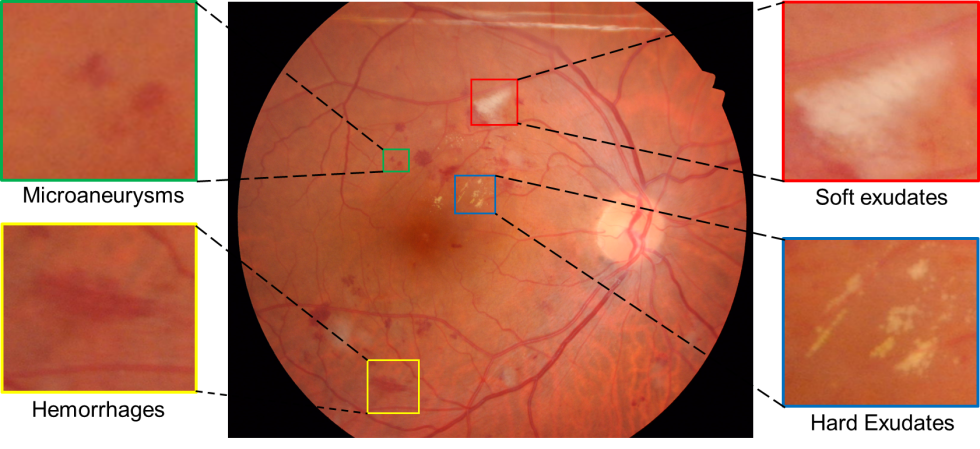
\includegraphics[width=1.0\textwidth]{figure/biomarker_localization_example}
	\caption{生物标记物定位任务示例。红色矩形框、绿色矩形框、蓝色矩形框和黄色矩形框标记了四种糖尿病视网膜病变的异常表现,分别代表软性渗出液(Soft Exudates)、微动脉瘤
		(Microaneurysms)、硬性渗出液(Hard Exudates)和出血(Hemorrhages)。} 
	\label{fig:biomarker_localization_example}
\end{figure}
生物标志物是开发新疗法和辅助诊断的关键,受到研究人员的不断关注,其目标是为合适的病人开发合适的药物。随着计算机视觉技术不断应用到医学领域,生物标记物定位任务自然也变成了研究热点。在医学影像处理领域,一旦一张医学影像被诊断为某种特定疾病,生物标记物定位任务的目标便是寻找其患病区域,或者说在图像上找到诊断依据,该依据或者患病区域即可看作是生物标记物。如图\ref{fig:biomarker_localization_example},该图像被诊断为患有糖尿病视网膜病变,生物标记物定位任务便是找到其异常表现,并给出其准确位置。可以发现,糖尿病视网膜病变有多种异常表现,生物标记物定位任务要求不能漏检。另外,可以发现从颜色特征上看,出血(图中黄色矩形框)异常和眼底血管非常相似,因而将微小血管看作异常表现的假阳现象也可能发现。以上均给生物标记物定位任务增加了不少难度。如果将卷积神经网络手段,根据以上介绍,生物标记物定位任务的目标是找出疾病诊断背后的诊断依据,这与卷积神经网络的可视化/可解释性的目标恰好一致,因此卷积神经网络的可视化/可解释性是生物标记物定位任务的主要解决方案之一。相关内容将会在\ref{subsec:visulization_methods}小节详细叙述。
\subsection{卷积神经网络}
卷积神经网络最初是为了避免传统神经网络(多层感知机~\cite{gardner1998artificial})在处理图像时的缺点而提出的。多层感知机在处理图像数据时,多层感知机对每张输入图像中的每个像素点都使用一个感知器。对于较大的图像,权重的数量很快就变得难以管理。例如,对于一个有3个彩色通道的224$\times$224像素图像,大约需要训练150,000个权值。此时,多层感知机的训练将变得十分困难。另外,多层感知机不具备平移不变性。例如,如果一张猫出现在一张图像的左上角和另一张图像的右下角,多层感知机将假设猫总是出现在图片的这个位置。再加上,多层感知机在处理图像时需要将二维图像数据将会以一维向量形式存在,因此无法利用二维空间的相对位置信息。
\begin{figure}[h]
	\centering
	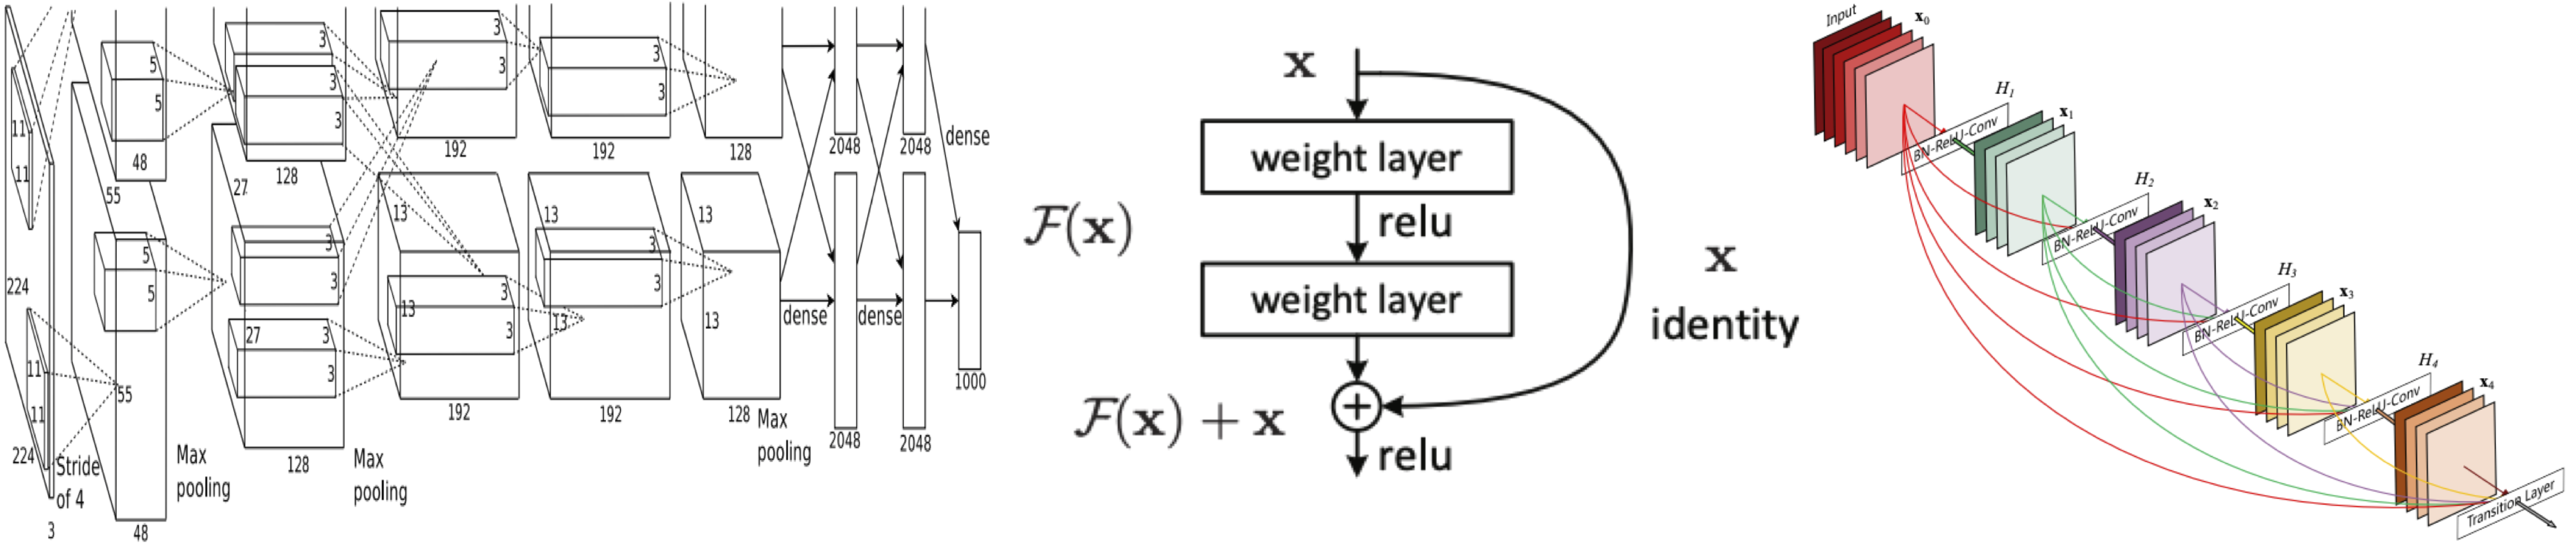
\includegraphics[width=1.0\textwidth]{figure/popular_networks}
	\caption{三种经典的卷积神经网络模型结构。从左到右,依次为AlexNet~\cite{krizhevsky2012imagenet}、ResNet~\cite{he2016deep, he2016identity}、DenseNet~\cite{huang2017densely}(图片均来自于原始论文)。注意,中间是ResNet的一个残差单元,ResNet实际上是由多个残差单元堆叠组成。} 
	\label{fig:popular_networks}
\end{figure}

卷积神经网络便可以很好避免多层感知机存在的问题,卷积操作可以很好的捕捉图像的空间信息。另外,卷机操作还具有平移不变性。权值共享机制可以大大降低参数量。随着计算机算力的快速提升,运用反向传播算法~\cite{hecht1992theory},卷积神经网络的大规模训练变得切实可行。自Hinton等人利用两块GPU成功训练AlexNet~\cite{krizhevsky2012imagenet}后,很多优秀网络结构被提出,比如VGG~\cite{simonyan2014very},ResNet~\cite{he2016deep, he2016identity},DenseNet~\cite{huang2017densely},Inception系列网络~\cite{szegedy2015going, szegedy2016rethinking, szegedy2017inception}。卷积神经网络除了在分类问题上取得出色性能外,还在自然语言处理~\cite{dos2014deep, mou2016convolutional, li2019knowledge}、无人驾驶~\cite{lee2017deep, csillik2018identification, tang2017vehicle}、语音识别~\cite{abdel2013exploring, swietojanski2014convolutional, robertson2019exploring}等领域表现不凡,越来越受到研究者们的青睐。

三种经典的卷积神经网络的模型结构如图~\ref{fig:popular_networks}所示。可以看出,卷积神经网络都是由一系列卷积操作组成的,在卷积操作之后再接上激活函数以增强非线性表达能力。为了减少参数量,卷积神经网络还引入了池化操作,使得输入图像尺寸随着深度不断增加而减小。池化操作也起到过滤无用信息的的作用。最后,再接上全连接层对卷积神经网络提取到的特征进行分类(视不同任务而改变)。因此,卷积神经网络实际上充当特征提取器的角色。那么我们可以这样理解卷积神经的原理:单纯卷积操作提取的是图像的局部信息,随着一系列卷积操作的堆叠,卷积神经网络的感受野越来越大,比如两个3$\times$3的卷积核堆叠相当于一个5$\times$5卷积核的感受野,卷积神经网络便能提取到图像的全局信息。同时,随着深度增加,输入的尺寸大小变得越来越小,通常以2倍关系减小,卷积神经网络便会丢掉无用信息。因而卷积神经网络是一种层次化结构。再在损失函数,如交叉熵,的监督指导下,根据反向梯度传播算法更新网络参数,卷积神经网络便能被训练成一个优秀的特征提取器。

以上便是卷积神经网络的一般结构和工作原理,下面详细介绍ResNet。随着VGG-19~\cite{simonyan2014very}的出现,一个卷积神经网络的深度越深,学出来的效果是否越好的问题摆在了研究者们的面前。由于卷积神经网络的深度越深,原本就存在的过拟合和梯度消失问题变得越严重。何凯明等人便设计了一种在深度远大于VGG-19,效果也由于VGG-19的网络模型。设$\mathcal{H}(x)$是卷积神经网络拟合的函数,$x$表示网络输入。如果假设多个非线性层可以渐近逼近复杂函数并且假设输入和输出尺寸相同,那么就可以假设它们可以渐近逼近残差函数$\mathcal{F}(x)$,即$\mathcal{F}(x)=\mathcal{H}(x)− x$。因此,ResNet没有让网络直接拟合$\mathcal{H}(x)$,而是明确地让这些层近似为残差函数$\mathcal{F}(x)=\mathcal{H}(x)-x$。 因此,原始函数变为$\mathcal{F}(x)+x$。尽管两种形式都应能够渐近地逼近所需的功能(如假设),但是近似拟合残差函数要容易得多。另外,为了表示加号,残差单元中通常加入跳接操作。

设$x_l$表示第$l$个残差单元的输入,$\mathcal{W}_{l}=\{\mathcal{W}_{l,k}|_{1\leq k \leq K}\}$表示第$l$个残差单元的权重,$K$表示残差单元个数。则相邻的残差单元输入$x_{l+1}$可以表示为:
\begin{gather}
	y_{l}=x_l + \mathcal{F}(x_l, \mathcal{W}_l), \\
	x_{l+1}=f(y_{l}).
\end{gather}
其中$f$表示激活函数,$\mathcal{F}(x_l, \mathcal{W}_l)$表示残差单元中的卷积操作。如果$f$表示恒等变换,则$x_{l+1}=y_{l}$,有:
\begin{equation}
	x_{l+1}=x_l + \mathcal{F}(x_l, \mathcal{W}_l).
\end{equation}
对于任意第$L(L\ge l)$个残差单元,其输入$x_{L}$,可写为:
\begin{equation}\label{residual_block_compute}
x_{L}=x_l + \sum_{i=l}^{L-1}\mathcal{F}(x_i, \mathcal{W}_i).
\end{equation}
设损失函数为$\varepsilon$,根据等式\ref{residual_block_compute}和反向梯度传播算法的链式求导法有:
\begin{equation}\label{residual_block_gradient}
\frac{\partial \varepsilon}{\partial x_l}=\frac{\partial \varepsilon}{\partial x_L}\frac{\partial x_L}{\partial x_l}=\frac{\partial \varepsilon}{\partial x_L}(1+\frac{\partial}{\partial x_l}\sum_{i=l}^{L-1}\mathcal{F}(x_i,\mathcal{W}_i)).
\end{equation}
等式\ref{residual_block_gradient}表明,梯度$\frac{\partial \varepsilon}{\partial x_l}$由$\frac{\partial \varepsilon}{\partial x_L}$和$\frac{\partial \varepsilon}{\partial x_L}\frac{\partial}{\partial x_l}\sum_{i=l}^{L-1}\mathcal{F}(x_i,\mathcal{W}_i)$两项组成。第一项在可直接传播信息而与任意残差单元无关。而第二项保证信息直接回传到上一个残差单元。由于第一项的存在,等式\ref{residual_block_gradient}还能保证每一层梯度不容易消失,即使在残差单元权重很小的情况下。而ResNet更是实现了在深度达到上千层的情况下,仍不会发生梯度消失现象。DenseNet更是将ResNet中提出的跳接扩展到了网络单元之间,正是由于ResNet的优异性能,本文卷积神经网络分类器使用ResNet-18。
\subsection{编码器-解码器}
\begin{figure}[h]
	\centering
	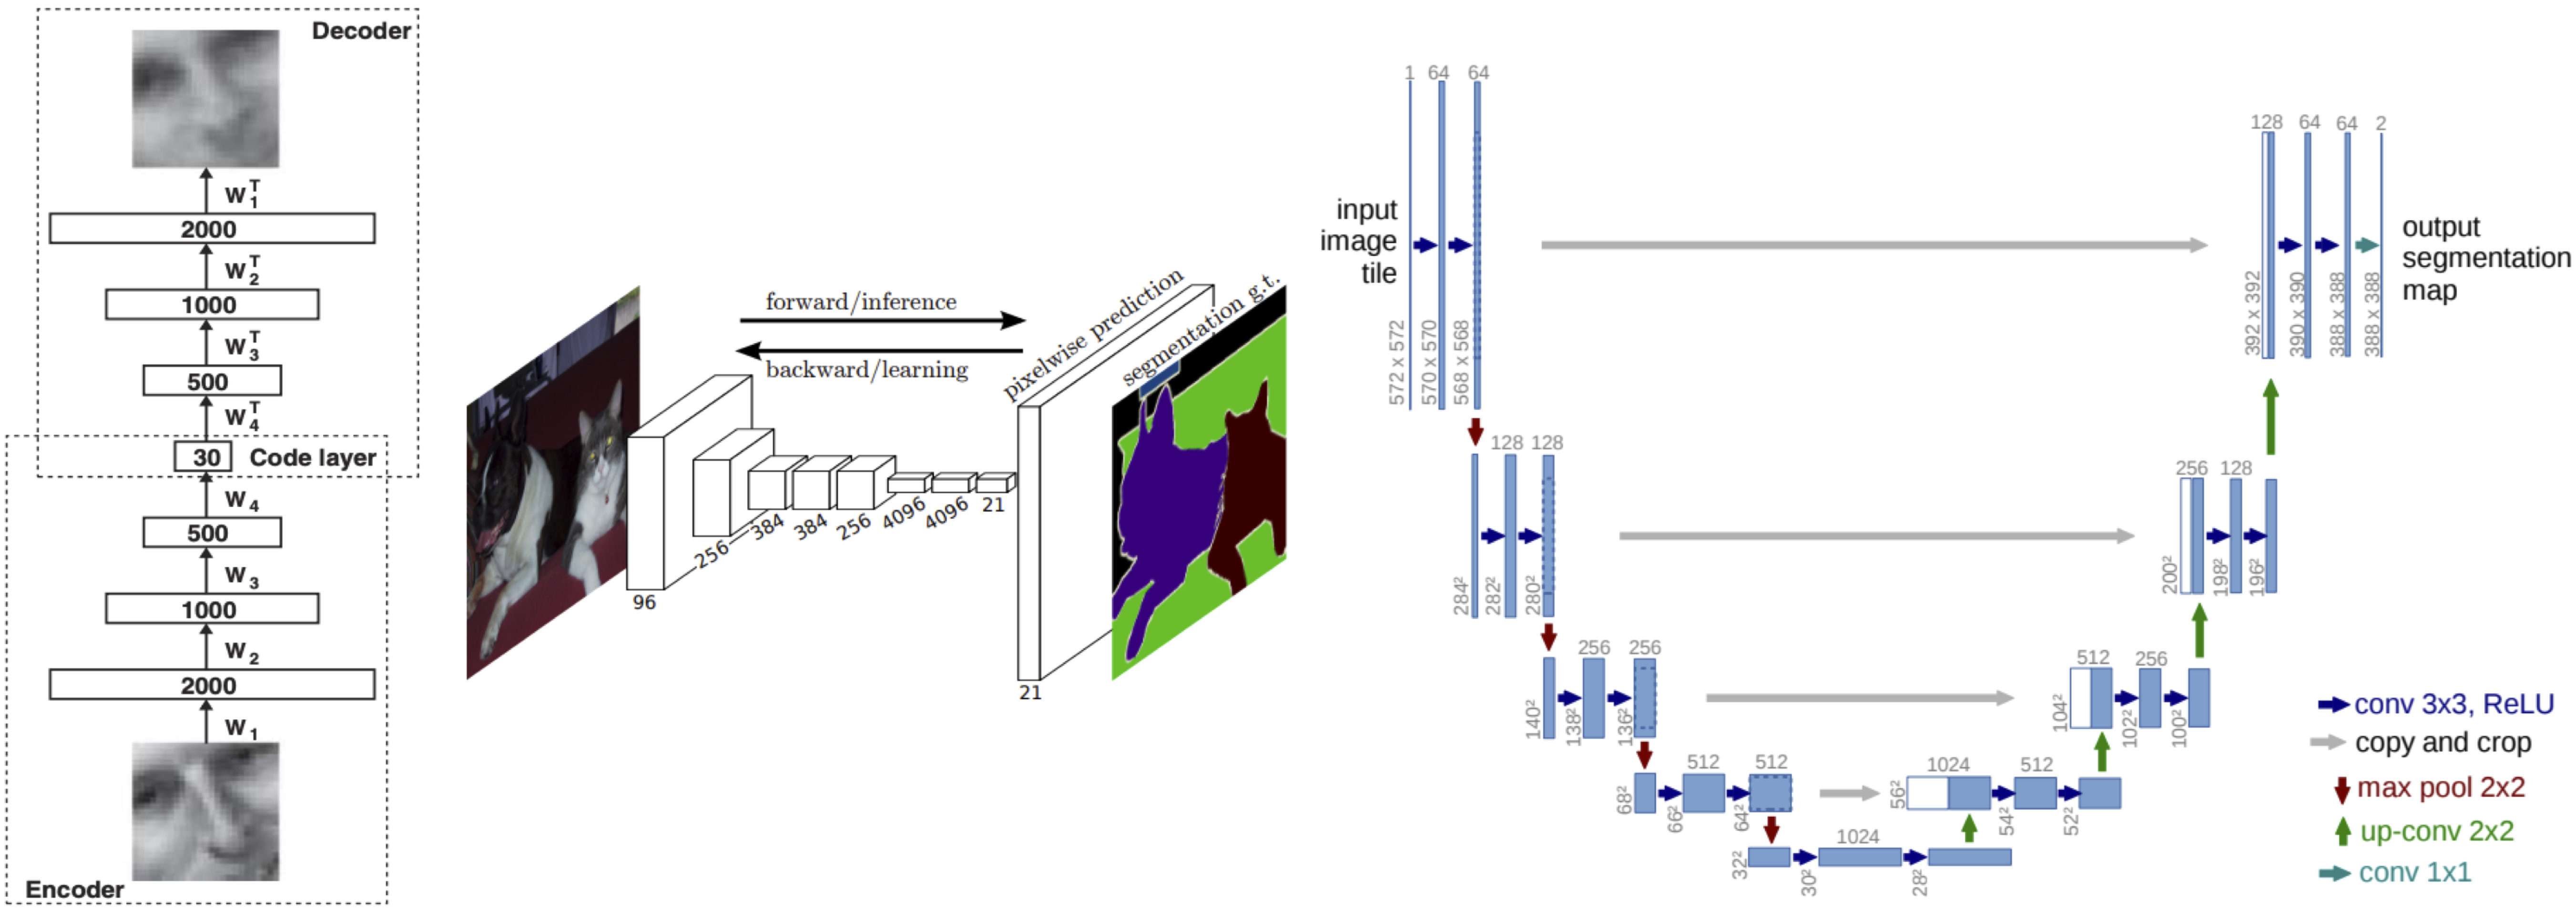
\includegraphics[width=1.0\textwidth]{figure/popular_encoder_decoder}
	\caption{三种经典的编码器-解码器模型结构。从左到右依次为编码器-解码器~\cite{hinton2006reducing}、全卷积神经网络~\cite{long2015fully}和U-Net~\cite{ronneberger2015u}(图片均来自于原文)。} 
	\label{fig:popular_encoder_decoder}
\end{figure}
编码-解码器自Hinton等人~\cite{hinton2006reducing}提出以来被广泛应用。编码-解码器不是某一种网络,而是代表了一类网络。随后便有降噪编码器-解码器~\cite{vincent2008extracting}、稀疏编码器-解码器~\cite{coates2011analysis}、变分贝叶斯编码器-解码器~\cite{kingma2013auto}等变体。将卷积操作应用到编码器-解码器中,启发了FCN~\cite{long2015fully}、U-Net~\cite{ronneberger2015u}、FPN~\cite{lin2017feature}等经典网络结构。FCN和U-Net均是分割分割领域(包括自然图像和医学图像)最为基础的网络结构。为了读者对编码器-解码器模型结构由较为直观的认识,三种经典网络结构如图\ref{fig:popular_encoder_decoder}所示。

在深度学学习领域,编码器-解码器是一种无监督的神经网络。从图\ref{fig:popular_encoder_decoder}可看出,编码器-解码器共同特点是由编码器和解码器组成,下面展开简要介绍:

1)编码器:编码器在网络结构图中是将卷积操作输入不断变小的过程,U-Net中是运用池化层实现下采样,不断将卷积操作输入以2倍关系缩小,从而达到提取图像特征的目的。由于通过编码器,可将输入维度不断降低,因此编码器-解码器最直观的应用便是图像压缩和图像去燥。在实际使用过程中,为了让编码器提取到输入较好的特征表达,通常会利用深度学习网络知识可迁移的优点,用Image-Net~\cite{deng2009imagenet}上的预训练模型参数来初始化编码器~\cite{iglovikov2018ternausnet}。

2)解码器:解码器和编码器相反,是将特征不断扩大,最终恢复到原图像大小的过程。通常会使用上采样或者反卷积~\cite{zeiler2010deconvolutional}操作以2倍关系逐步扩大,从而达到融合不同层次、不同尺寸的特征的目的。

由于本文使用到了U-Net~\cite{ronneberger2015u},故同时简单介绍U-Net。除了以上特点之外,U-Net中还存在从编码器直接到解码器的跨层连接,这些跨层连接使网络可以将上下文信息传播到更高分辨率的层,从而使得特征融合更加充分。在网络可视化图上(见图\ref{fig:popular_encoder_decoder}右子图),由于编码器和解码器相互对称,形成一个U型结构。U-Net中只含有卷积层,不含任何全连接层,最后视不同任务而接上不同激活函数。U-Net作为一种巧妙的网络模型,被广泛应用于医学影像处理领域~\cite{cciccek20163d, han2018framing, dong2017automatic, sevastopolsky2017optic, zhang2018ct},更多启发了诸多优秀网络模型~\cite{zhou2018unet++, oktay2018attention, ibtehaz2020multiresunet, alom2019recurrent, milletari2016v}。
\subsection{对抗生成网络}
对抗生成网络(Generative Adversarial Networks,缩写为GAN)最初于2014年由Goodfellow等人~\cite{goodfellow2014generative}提出,就越来越受到学术界和工业界的重视。而随着GAN在理论与模型上的高速发展,它在计算机视觉~\cite{zhu2017unpaired, isola2017image}、自然语言处理~\cite{qin2018dsgan, guimaraes2017objective}、人机交互~\cite{qiao2018emotional, sahu2018enhancing}等领域有着越来越深入的应用,在医学影像领域更是大放异彩~\cite{yang2017dagan, yang2018low, shin2018medical, onishi2020multiplanar, bhadra2020medical}。GAN是生成式模型,受博弈论中的零和博弈启发,将生成问题视作判别网络和生成网络这两个网络的对抗和博弈。生成网络努力生成新数据,判别器努力区分生成网络生成的数据(一般记为“假”)和真实数据(一般记为“真”)。生成网络尽量产生更真实的数据,而判别器尽量更完美地把真实数据与生成数据区分开来。由此,生成网络和判别器形成对抗关系,彼此进步。在不断的迭代训练过程中,生成网络生成的数据也就越来越逼近真实数据,即生成网络学到的分布越来越接近真实数据代表的分布。在理想情况下,判别器无法区分生成的数据和真实的数据。

设真实数据为$x\sim p_{data}(x)$,噪音为$z\sim p_z(z)$,生成网络和判别网络分别用$G$和$D$表示。$\theta_{g}$和$\theta_{d}$分表表示$G$和$D$的训练参数。则$G(z;\theta_{g})$表示生成网络生成的函数映射。$D(x;\theta_{d})$将会输出一个数值。可将$D$看做一个二类分类器。不妨将交叉熵当做损失函数。因此,可用$D(x)(0\leq D(x)\leq 1)$表示数据$x$来自于真实数据的概率。运用极大极小优化理论,GAN的损失函数可写成:
\begin{equation}\label{equ:gan_loss_func}
\min _{G} \max _{D} V(D, G)=\mathbb{E}_{\boldsymbol{x} \sim p_{\text {data }}(\boldsymbol{x})}[\log D(\boldsymbol{x})]+\mathbb{E}_{\boldsymbol{z} \sim p_{\boldsymbol{z}}(\boldsymbol{z})}[\log (1-D(G(\boldsymbol{z})))].
\end{equation}
我们对$D$进行训练,使其对$G$中的训练示例和样本分配正确标签的概率最大化。我们同时对$G$进行训练,使其对$log(1 - D(G(z))$最小化。换句话说,$D$和$G$玩了一个具有损失函数$V (G, D)$的二人极大极小博弈。在实际训练时,$D$和$G$先后交替训练。

\noindent 固定$\theta_{g}$,优化$\theta_{d}$等价于用随机梯度上升算法最大化损失函数:
\begin{equation}\label{equ:g_updated_loss_func}
\log D\left(x\right)+\log \left(1-D\left(G\left(z\right)\right)\right).
\end{equation}

\noindent 固定$\theta_{d}$,优化$\theta_{g}$等价于用随机梯度下降算法最小化损失函数:
\begin{equation}
\log \left(1-D\left(G\left(z\right)\right)\right).
\end{equation}
\noindent 在Goodfellol提出以上朴素GAN在生成网络和判别网络均是多层感知机。在实际训练过程中参数过大,训练难度较大的问题,因而训练不稳定,经常训练失败。各种改进模型相继提出,DCGAN~\cite{radford2015unsupervised}利用了卷积神经网络强大的拟合能力和容量。针对训练过程中存在的梯度消失问题,WGAN~\cite{gulrajani2017improved}使用Wasserstein-1距离代替GAN~\cite{goodfellow2014generative}中的Jensen-Shannon散度~\cite{arjovsky2017towards}。WGAN-GP~\cite{gulrajani2017improved}更是在WGAN基础上又在GAN损失函数(见等式\ref{equ:gan_loss_func})中加入了梯度惩罚项(Gradient Penalty),这也是WGAN-GP名字的由来。由于WGAN-GP可以有效避免GAN训练过程中的梯度消失,本文网络模型中GAN采用的就是WGAN-GP,下面进行简单简单介绍。

与朴素GAN~\cite{goodfellow2014generative}不同的是,在WGAN-GP中,判别器不再被看作是二分类器,而是近似去拟合Wasserstein-1距离,属于回归任务,因此也会去掉朴素GAN中判别器最后一层的Sigmoid激活函数。设$p_g$表示给定噪音分布$z\sim p_z$时生成网络所代表的的分布。再加上梯度惩罚项,WGAN-GP的损失函数可写作:
\begin{equation}\label{wgan_gp_loss_func}
\min _{G} \max _{D} V(D, G)=E_{x \sim P_{d a t a}}[D(x)]-E_{x \sim p_{g}}[D(x)]+\lambda E_{\hat{x} \sim p_{\hat{x}}}\left[\left(\left\|\nabla_{\hat{x}} D(\hat{x})\right\|_{2}-1\right)^{2}\right].
\end{equation}
其中,$\lambda$为梯度惩罚项的权重,分布$p_{\hat{x}}$不是对整个样本空间采样,而只对分布$p_{data}$和分布$p_{g}$之间的空间采样。在训练时同样$D$和$G$先后交替训练。因此,固定$G$,更新$\theta_{d}$时,等效于最小化损失函数:
\begin{gather}
\tilde{{x}} = G_{}({z}), \\
D(\tilde{{x}})-D({x})+\lambda\left(\left\|\nabla_{\hat{x}} D(\hat{x})\right\|_{2}-1\right)^{2}.
\end{gather}
\noindent 固定$D$,更新$G$时,等效于最小化损失函数:
\begin{equation}
-D\left(G_{\theta}(z)\right).
\end{equation}
通过实验证明,WGAN-GP在训练过程中梯度较为稳定,不易发生梯度消失现象。另外,Wasserstein-1距离还能指示WGAN-GP训练效果的作用,Wasserstein-1距离越大,表示WGAN-GP训练得越好,使得训练过程易于理解。
\section{生物标记物定位方法}
随着计算机计算在医学影像领域的广泛应用,目前已有可用于生物标记物定位的模型提出,主要包括多示例学习~\cite{maron1998framework}和卷积神经网络的可视化方法~\cite{zhou2016learning, selvaraju2017grad}。本小节将对其中的经典方法进行详细介绍,并比较方法之间的优劣,以便于读者对这些方法有清晰的认识与理解。
\subsection{多示例学习}
多示例学习~\cite{maron1998framework}
\subsection{卷积神经网络的可视化}\label{subsec:visulization_methods}
%\section{评价标准}
%\section{本章小结}
        % \newclearpage
        \chapter{疾病标记物的自动定位方法}\label{sec:method}
%\section{前言}
%随着深度学习渗透到医学影像分析领域的方方面面,疾病标记物定位任务也受到研究者的持续关注,其性能也在稳步提升。然而正如\ref{subsec:related_work_summary}小结所描述的,由于目前已有方法由于自身原因无法精确定位疾病标记物位置,因而无法达到令人满意的性能。
有鉴目前已有的相关工作无法实现疾病标记物的精确定位(相关内容参见\ref{sec:related_work}小节),本文将提出一种新颖的网络模型和训练方法,以期达到精确定位疾病标记物的目的。具体而言,在\ref{sec:idea_thinking}小节,本文将解释我们的对于此问题的思考,叙述本文的研究问题和我们的解决思路,以期读者能更好地理解本文提出的方法。接着,在\ref{sec:model_architecture_intro}小节中,本文将介绍模型结构,包括各个子模块和各自充当的角色。随后,我们将在\ref{sec:loss_func_training_stragies}小节中定义模型的损失函数、训练步骤以及网络更新策略。

\section{研究问题与解决思路}\label{sec:idea_thinking}
\subsection{研究问题}
在医学图像中,疾病标记物具有极强的临床应用价值,可用于处理疾病诊断、疾病风险预测、疾病类型区分等问题,精确定位疾病标记物则是首要一步。在医学图像中,如果疾病标记物分布广泛,其边界模糊,其尺寸大小与数量不一,像素级标注往往代价非常高昂甚至不具备实际可行性。鉴于以上情况,本文旨在在弱监督条件下精确定位医学图像中分布广泛、边界模糊、尺寸大小与数量不一的疾病标记物。
\subsection{解决思路}
面对弱监督条件下,疾病标记物的精确定位这一问题,鉴于已有方法只能粗略定位到疾病标记物,我们可用生成对抗网络思路去做,保证输入输出图像尺寸相等,以避免上采样所带来的定位不够精确问题,训练完成之后,GAN中的生成器输出减去对应输入即可定位图像中的疾病标记物。我们期望本文设计的GAN具有以下能力:

1)如果输入图像是正常图像,那么生成器输出图像与输入图像保持一致,即此时输入图像并没有像素强度发生改变。
	
2)如果输入图像是异常图像,可以想象,如果生成器输出图像与输入图像相比,只有极少数像素强度发生改变,而绝大部分像素强度没有发生改变,那么我们完全有理由认为这些发生改变了的像素便是疾病标记物,此时我们可以认为生成器输出图像是异常输入图像去除疾病标记物之后的“正常”版本,且疾病标记物的准确位置可由生成器输出图像减去输入图像给出。

\noindent 一旦GAN具有以上功能,我们就可以很好地定位图像中的疾病标记物。考虑到GAN在图像中能较好去除遮挡物,如去除单张图像中的雨滴~\cite{qian2018attentive}(见图\ref{subfig:attention_gan}),去除人脸中的遮挡物~\cite{yuan2019face}(见图\ref{subfig:face_de_occulusion}),尤其是对于雨滴这种相对较小、分布较为广泛的物体仍能处理得相当好,这足以证明GAN强大的图像生成能力,因此我们可借助GAN的图像生成能力,去除医学图像中的疾病标记物。
\begin{figure}[h!]
	\begin{subfigure}{0.45\textwidth}
		\centering
		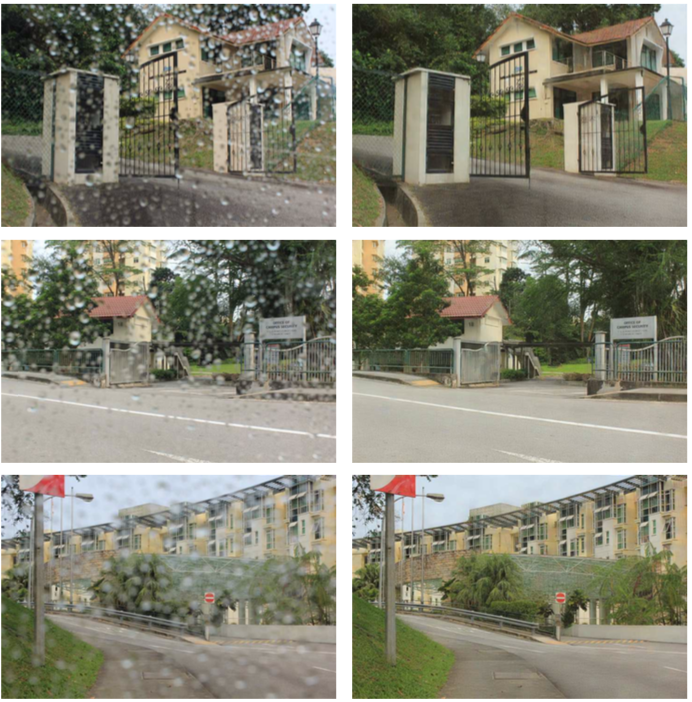
\includegraphics[width=0.75\textwidth]{figure/attention_gan_example.png}
		\caption{GAN去除图像中的雨滴~\cite{qian2018attentive}。}
		\label{subfig:attention_gan}
	\end{subfigure}
	\begin{subfigure}{0.45\textwidth}
		\centering
		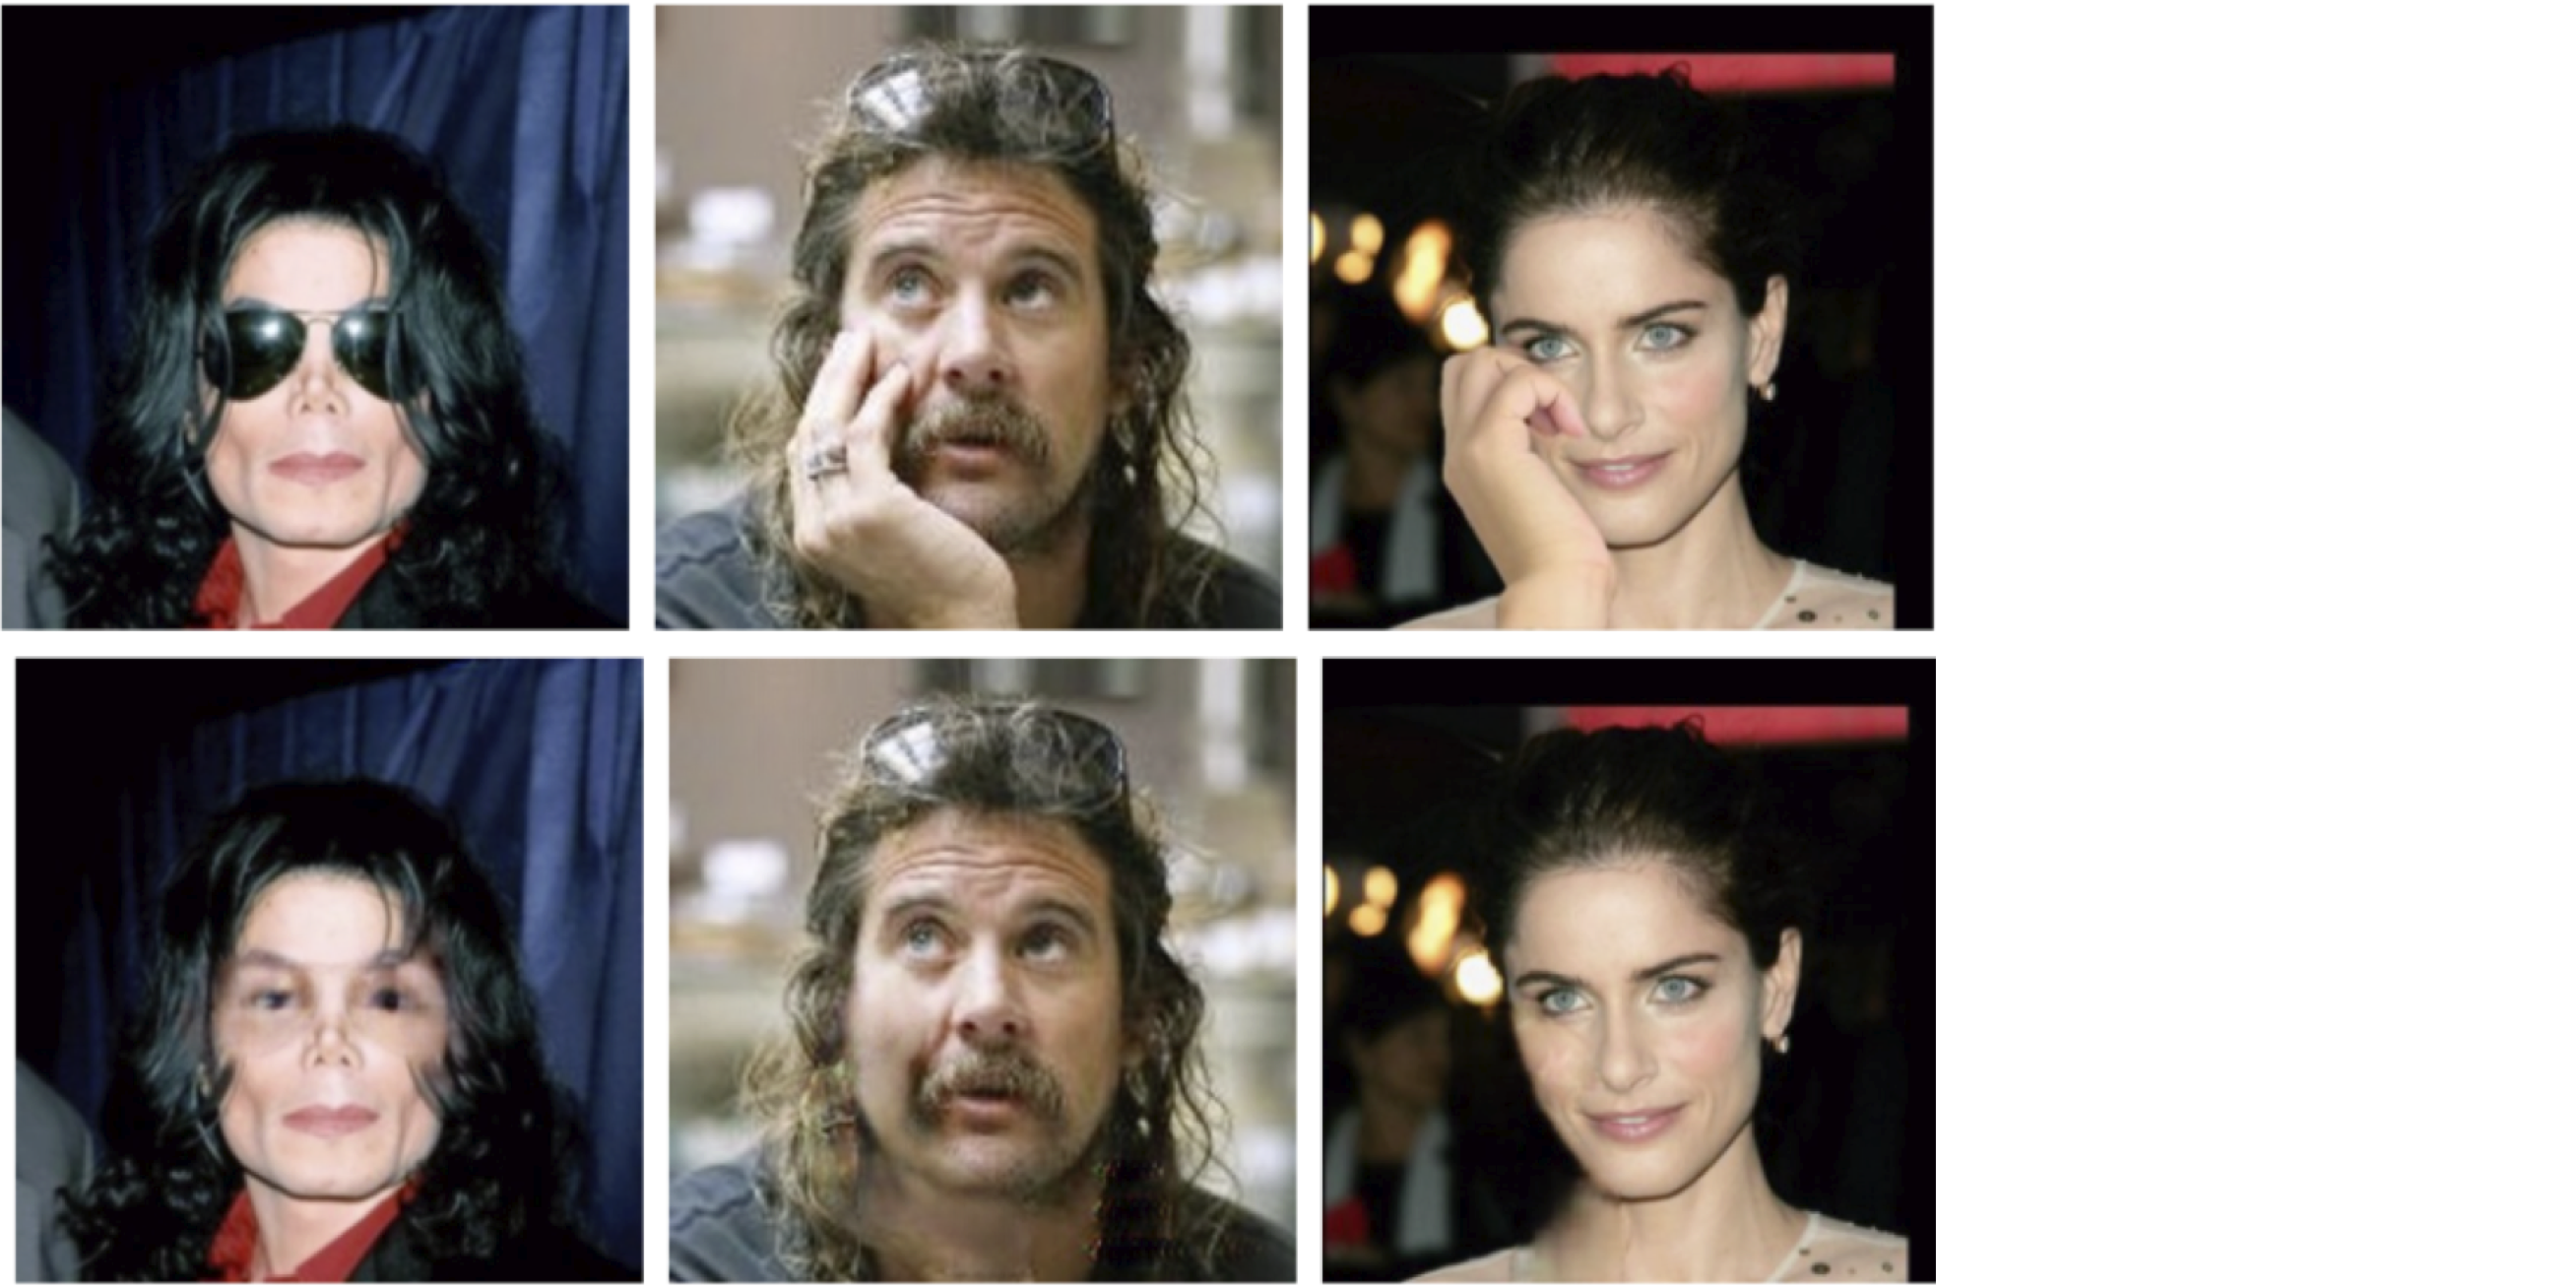
\includegraphics[width=1.5\textwidth]{figure/face_de_occulusion.png}
		\caption{GAN去除人脸中的遮挡物~\cite{yuan2019face}。}
		\label{subfig:face_de_occulusion}
	\end{subfigure}
	\caption[GAN去除图像中遮挡物示例]{GAN去除图像中遮挡物示例(图片均来自于对应原文~\cite{qian2018attentive,yuan2019face})。}
	\label{mul_fig:gan_auto_encoder_example}
\end{figure}

%\paragraph{解决思路} 面对弱监督条件下,疾病标记物的精确定位这一问题,鉴于已有方法只能粗略定位到疾病标记物,我们最先想到用图像生成即对抗生成网络的思路去做,并且输入输出图像尺寸相等,这样就避免了CAM和Grad-CAM中由于上采样所造成的定位不精确的问题。如果用映射$H$来表示生成器,给定输入图片$I^{h\times w\times d}$(图像的高、宽和深度分别为$h$,$w$,$d$),则$H$是一个图像到图像的映射,可形式化为:
%\begin{equation*}
%H: I \to I'.
%\end{equation*}
%其中$I'^{h\times w\times d}$与$I$一样,均表示一张图像。假设生成器有识别疾病标记物或者说患病区域的能力,不难想象,在理想状态下,给定输入图像$I$,生成器给出其输出图像$I'$,根据输入图像类别是正常还是异常,有以下推断:

%\noindent 1)如果输入图像$I$是正常图像,则可认为输出图像$I'$与输入图像$I$一致,即此时输入图像并没有像素强度发生改变。

%\noindent 2)如果输入图像$I$是异常图像,可以想象,与输出图像$I'$相比,输入图像$I$中只有极少数像素强度发生改变,而绝大部分像素强度没有发生改变,那么我们完全有理由认为这些发生改变了的像素便是疾病标记物,此时我们可以认为输出图像$I'$是异常输入图像$I$去除疾病标记物的“正常”版本,且疾病标记物的准确位置$Y$为:
%\begin{equation}\label{equ:idea}
%Y=|I'-I|=|H(I) - I|.
%\end{equation}
%\noindent 根据等式\ref{equ:idea},一旦得到这样的生成器,便可以实现疾病标记物的精确定位。根据以上设计,可知生成器满足以下两个条件:
%\begin{itemize}\label{item:satified_conditions}
%	\item 给定输入图像$I$,生成器能生成具有与输入图像大小相同的输出图像$I'$。 
%	\item 生成器具有良好的识别疾病标记物的能力。
%\end{itemize}
%\noindent 对于条件一,实现比较容易,全卷积网络或者编码器-解码器,都能满足这一条件。考虑到近些年来编码器-解码器在图像生成领域所取得的巨大成就,我们优先考虑选择编码器-解码器。主要难点在于第二点:如何让编码器-解码器具备识别疾病标记物或者说异常信号的能力。编码器-解码器作为一种无监督模型,最朴素的想法是只使用正常图像训练编码器-解码器,使其具有重建正常图像或者说正常信号的能力,当送入异常图像时,由于编码器-解码器并未见过异常信号,故编码器-解码器无法较好重建异常信号,从而间接使编码器-解码器具有识别异常信号的能力。实际上,在单张图像中,由于疾病标记物所占的像素在整张图像中只占很小一部分($\le 2\%$),再加上CNN强大的拟合能力和高容量,这种位于局部的图像细节差异往往非常不明显,很难被凸显出来。因此,需要引入其他模块来指导编码器-解码器,在弱监督条件下,图像级标签是有提供的,故可引入一个CNN分类器。根据以上设计(参见\ref{item:satified_conditions}小节中编码器-解码器满足的两个条件),如果编码器-解码器具备识别疾病标记物的能力,对于异常图像$I_{lesion}$和正常图像$I_{normal}$,在理想情况下,有:
%\begin{itemize}\label{ite:ideal_situation}
%	\item 对于输入图像$I_{lesion}$,输出图像$({H}(I_{lesion}))$与原输入图像比只有极少数像素强度发生改变,是其“正常”版本,故$({H}(I_{lesion})-I_{lesion})$仍含有原始图像$I_{lesion}$上的全部疾病标记物。 
%	\item 对于输入图像$I_{normal}$,输出图像${H}(I_{lesion})$与原输入图像比未发生像素强度的改变,仍为正常图像,故$({H}(I_{normal})-I_{normal})$不含有任何疾病标记物。
%\end{itemize}
%我们可以发现,对于输入图像$I$,无论$I$是正常图像还是异常图像,编码器-解码器的输出图像与输入图像之差$({H}(I)-I)$与原始图像$I$的标签是一致的,故我们可以试图通过引入一个CNN分类器完成一个分类任务来使编码器-解码器具备识别疾病标记物的能力,只是CNN分类器的输入不再是原始输入图像$I$,而是编码器-解码器的输出图像和原始输入图像之差,这样的取差操作还有一个好处是可以排除原始图像中无关信息(如背景)的干扰,让CNN分类器更加关注与疾病标记物相关的信息。此时的模型是编码器-解码器和CNN分类器的组合。但是,考虑到CNN分类器在做分类任务时,由于卷积操作感受野的局部性,CNN分类器可能是根据图像中最为突出、最为重要的图像模式或者特征进行分类的,比如说,一张图像中有很多只猫,固然CNN分类器能够正确完成分类,但是其分类依据极有可能是在图像中所占比例最大、毛色最突出的某一只或某几只猫,而没有考虑到甚至直接忽略在图像的某一角还有一只甚至几只相对不够突出的猫,这种情况在含有多个大小不一的目标物体的图像中是很有可能发生的。同理,如果一张医学图像$I_{lesion}$中含有多个大小不一、形状各异、分布广泛的疾病标记物,而编码器-解码器只有部分识别疾病标记物的能力,则其输入图像$I'_{lesion}$很可能只有部分相对不够明显的疾病标记物,则此时输出图像和输入图像的差$(I'_{lesion}-I_{lesion})$中只有相对比较明显的疾病标记物,显而易见,这种情况是能够骗过CNN分类器,使其作出此输入为异常的判断。注意,此时$(I'_{lesion}-I_{lesion})$只能定位到相对较为明显的疾病标记物而漏掉了相对不够明显的疾病标记物。显然,我们还需要更为精确的定位结果。

%鉴于以上情况,考虑到对抗生成网络与编码器-解码器的有效结合并在图像中能较好去除遮挡物,如去除单张图像中的雨滴~\cite{qian2018attentive}(见图\ref{subfig:attention_gan}),去除人脸中的遮挡物~\cite{yuan2019face}(见图\ref{subfig:face_de_occulusion})。尤其是对于雨滴这种相对较小、分布较为广泛的物体仍能处理的相当好,完全有理由考虑再引入对抗生成网络进一步帮助编码器-解码器去除图像中相对不够明显的疾病标记物。如果将编码器-解码器看做对抗生成网络中的生成器,那么只需额外引入一个判别器模块即可。此时,我们提出的模型由编码器-解码器、CNN分类器和判别器组成,其中,判别器和生成器共同组成了对抗生成网络。更多的模块引入,也就意味着需要更为精巧的组合方式和训练方式。接下来,本文\ref{sec:model_architecture_intro}小节将详细介绍整体模型结构和每个模块的模型结构。

%\begin{figure}[h!]
%	\begin{subfigure}{0.45\textwidth}
%		\centering
%		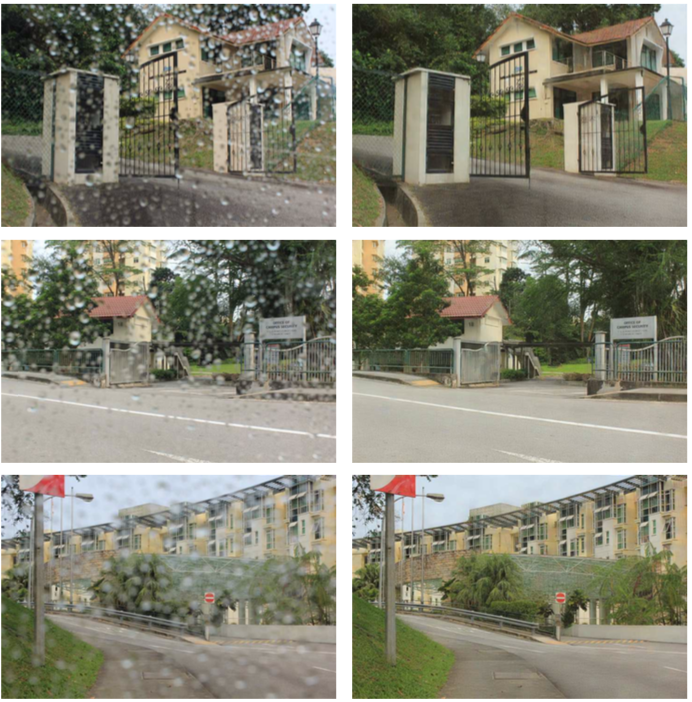
\includegraphics[width=0.75\textwidth]{figure/attention_gan_example.png}
%		\caption{去除单张图像中的雨滴(图片来自于原文)。}
%		\label{subfig:attention_gan}
%	\end{subfigure}
%	\begin{subfigure}{0.45\textwidth}
%		\centering
%		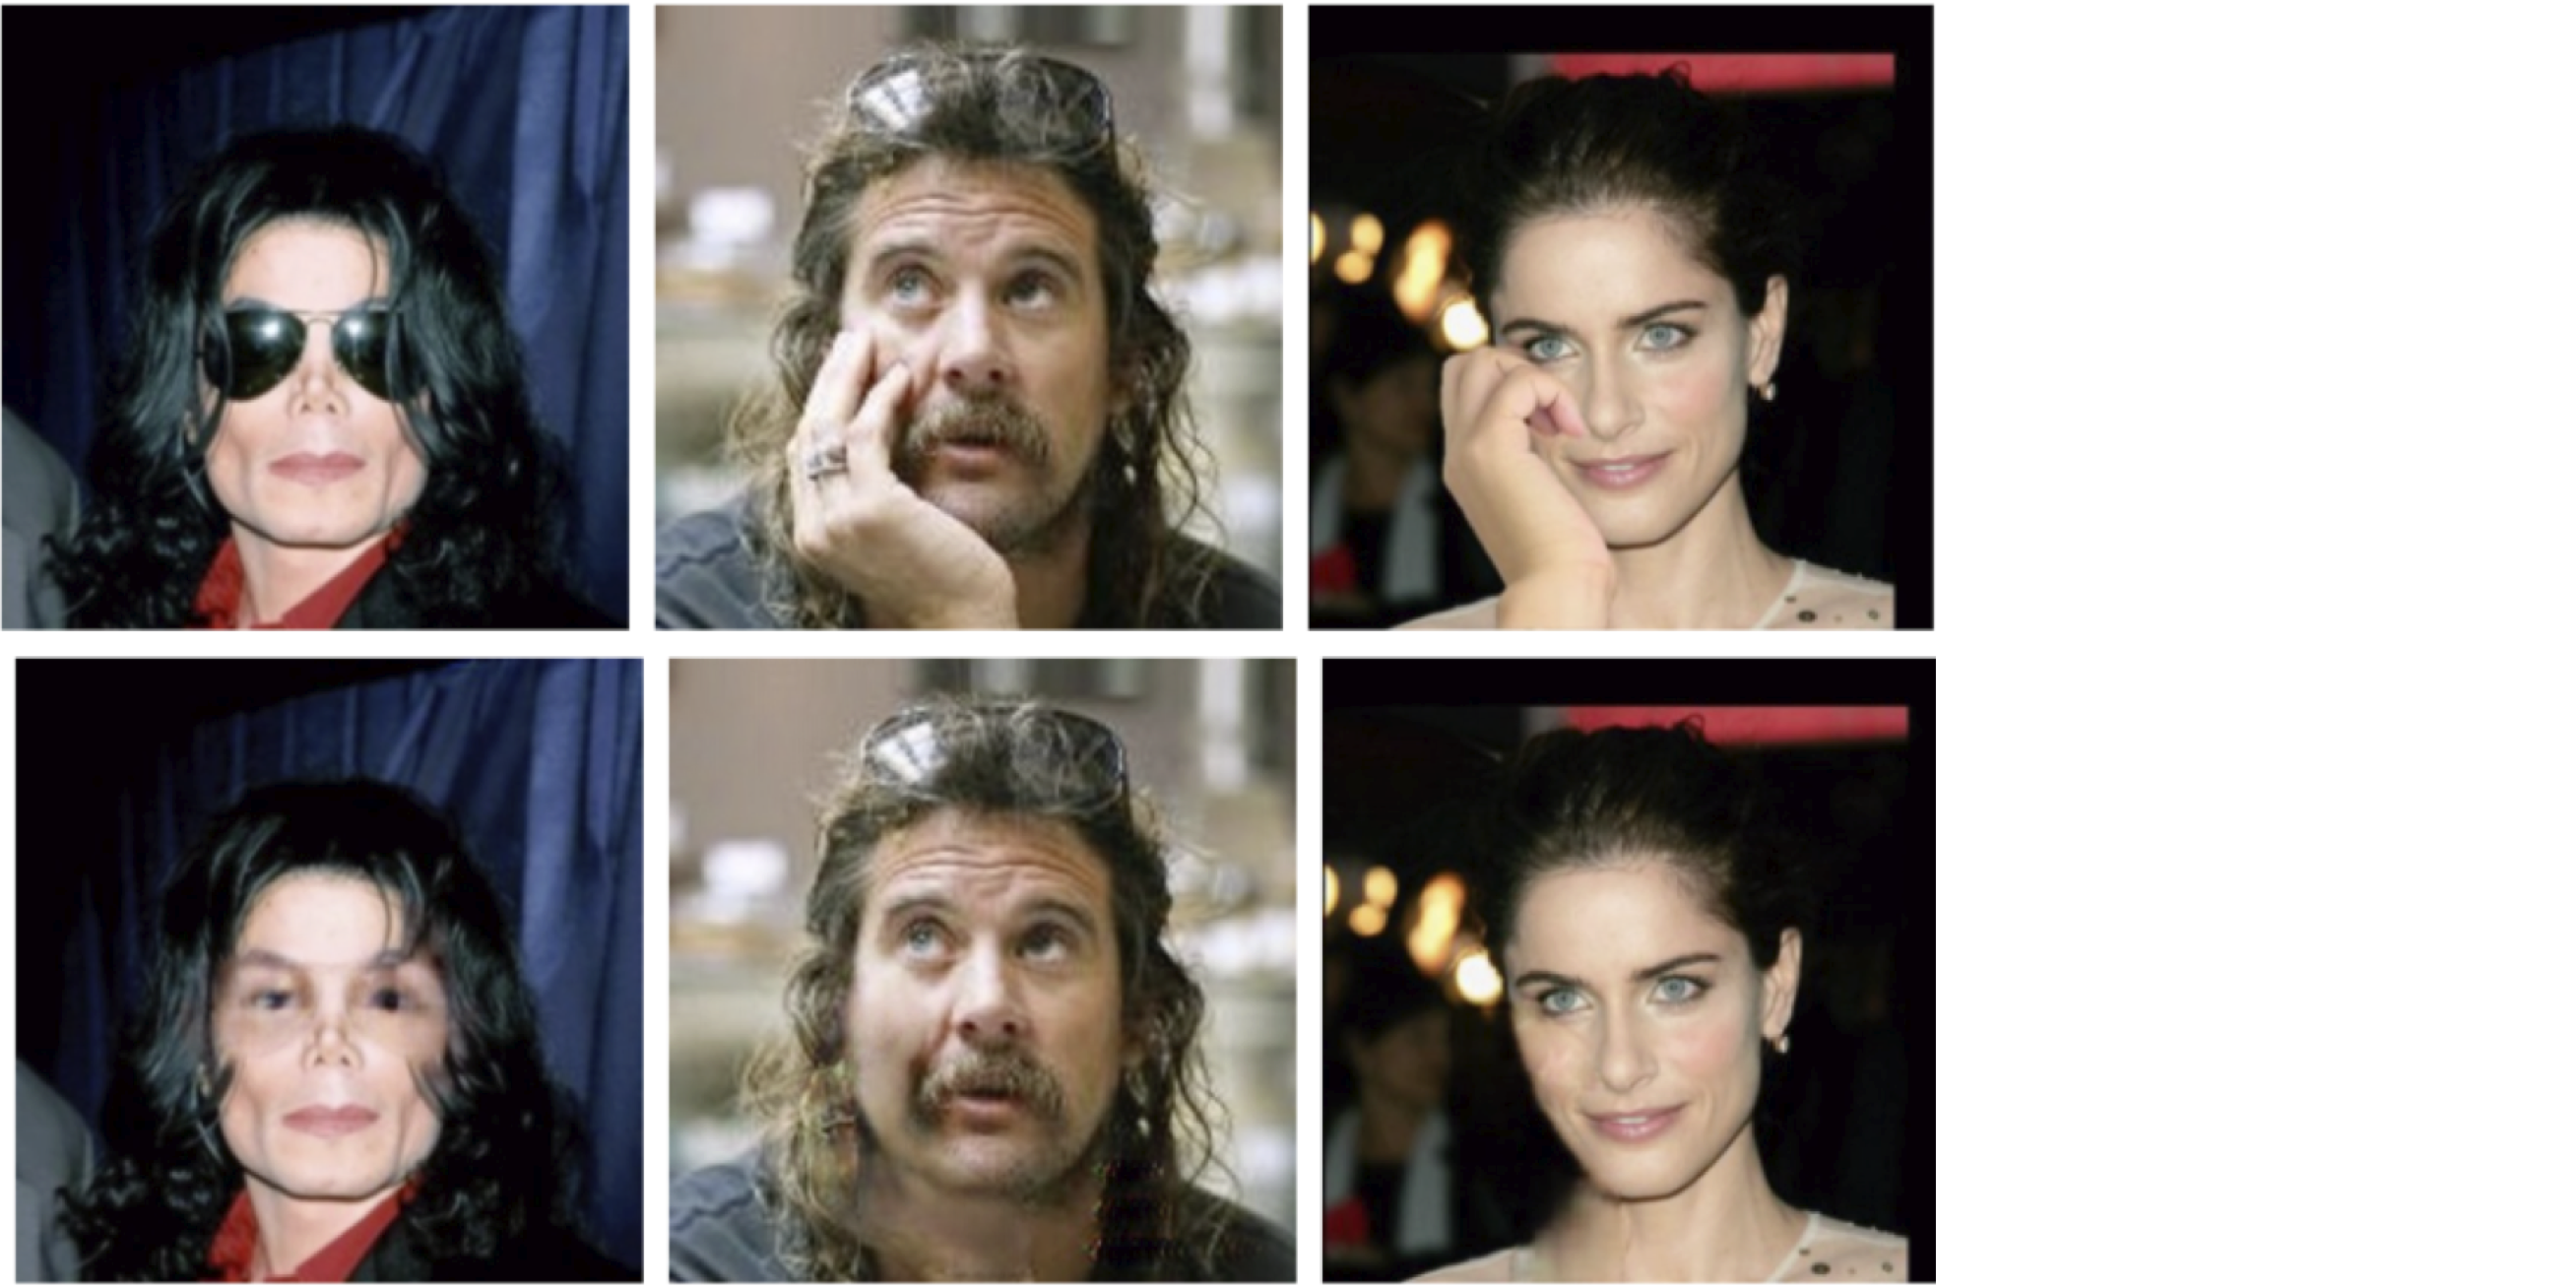
\includegraphics[width=1.5\textwidth]{figure/face_de_occulusion.png}
%		\caption{去除人脸中的遮挡物(图片来自于原文)。}
%		\label{subfig:face_de_occulusion}
%	\end{subfigure}
%	\caption{对抗生成网络与编码器-解码器的有效结合并在图像中能较好去除遮挡物示例。}
%	\label{mul_fig:gan_auto_encoder_example}
%\end{figure}

\section{模型结构介绍}\label{sec:model_architecture_intro}
在\ref{sec:idea_thinking}小节中,本文已经介绍了解决疾病标记物的解决思路和理论建模。本小节内容将详细介绍本文提出的疾病标记物定位模型和各个子模块的模型结构,力求读者能清晰明了地理解本文方法的核心思想。

%具体来说,本文将在\ref{subsec:model_architecture}小节中详细介绍整体模型结构及各个子模块在整体模型中所起到的作用和相互关系。接下来,在\ref{subsec:encoder_decoder_model}小节、\ref{subsec:cnn_classifier_model}小节和\ref{subsec:discrimintor_model}小节分别介绍编码器-解码器、CNN分类器和判别器的模型结构。下面展开相关内容的具体阐述。

\subsection{疾病标记物定位模型}\label{subsec:model_architecture}
本文提出的模型目的是在仅图像级别的标签可用时,精确定位异常图像中潜在的生物标志物或病变区域。我们的想法是设计一种可以学会直接查找疾病标记物的新架构。出于这种动机,我们提出了一种新颖的深度神经网络。这种网络结合了两种不同的学习架构(见图\ref{fig:our_model_architecture}):发挥监督作用的CNN分类器和负责图像生成的GAN(由编码器-解码器和判别器组成)。CNN分类器和判别器可以共同帮助编码器-解码器更有效地从输入图像中除去疾病标记物。训练完成后,可以通过编码器-解码器的输入中减去其输出来定位疾病标记物。
\begin{figure}[h]
	\centering
	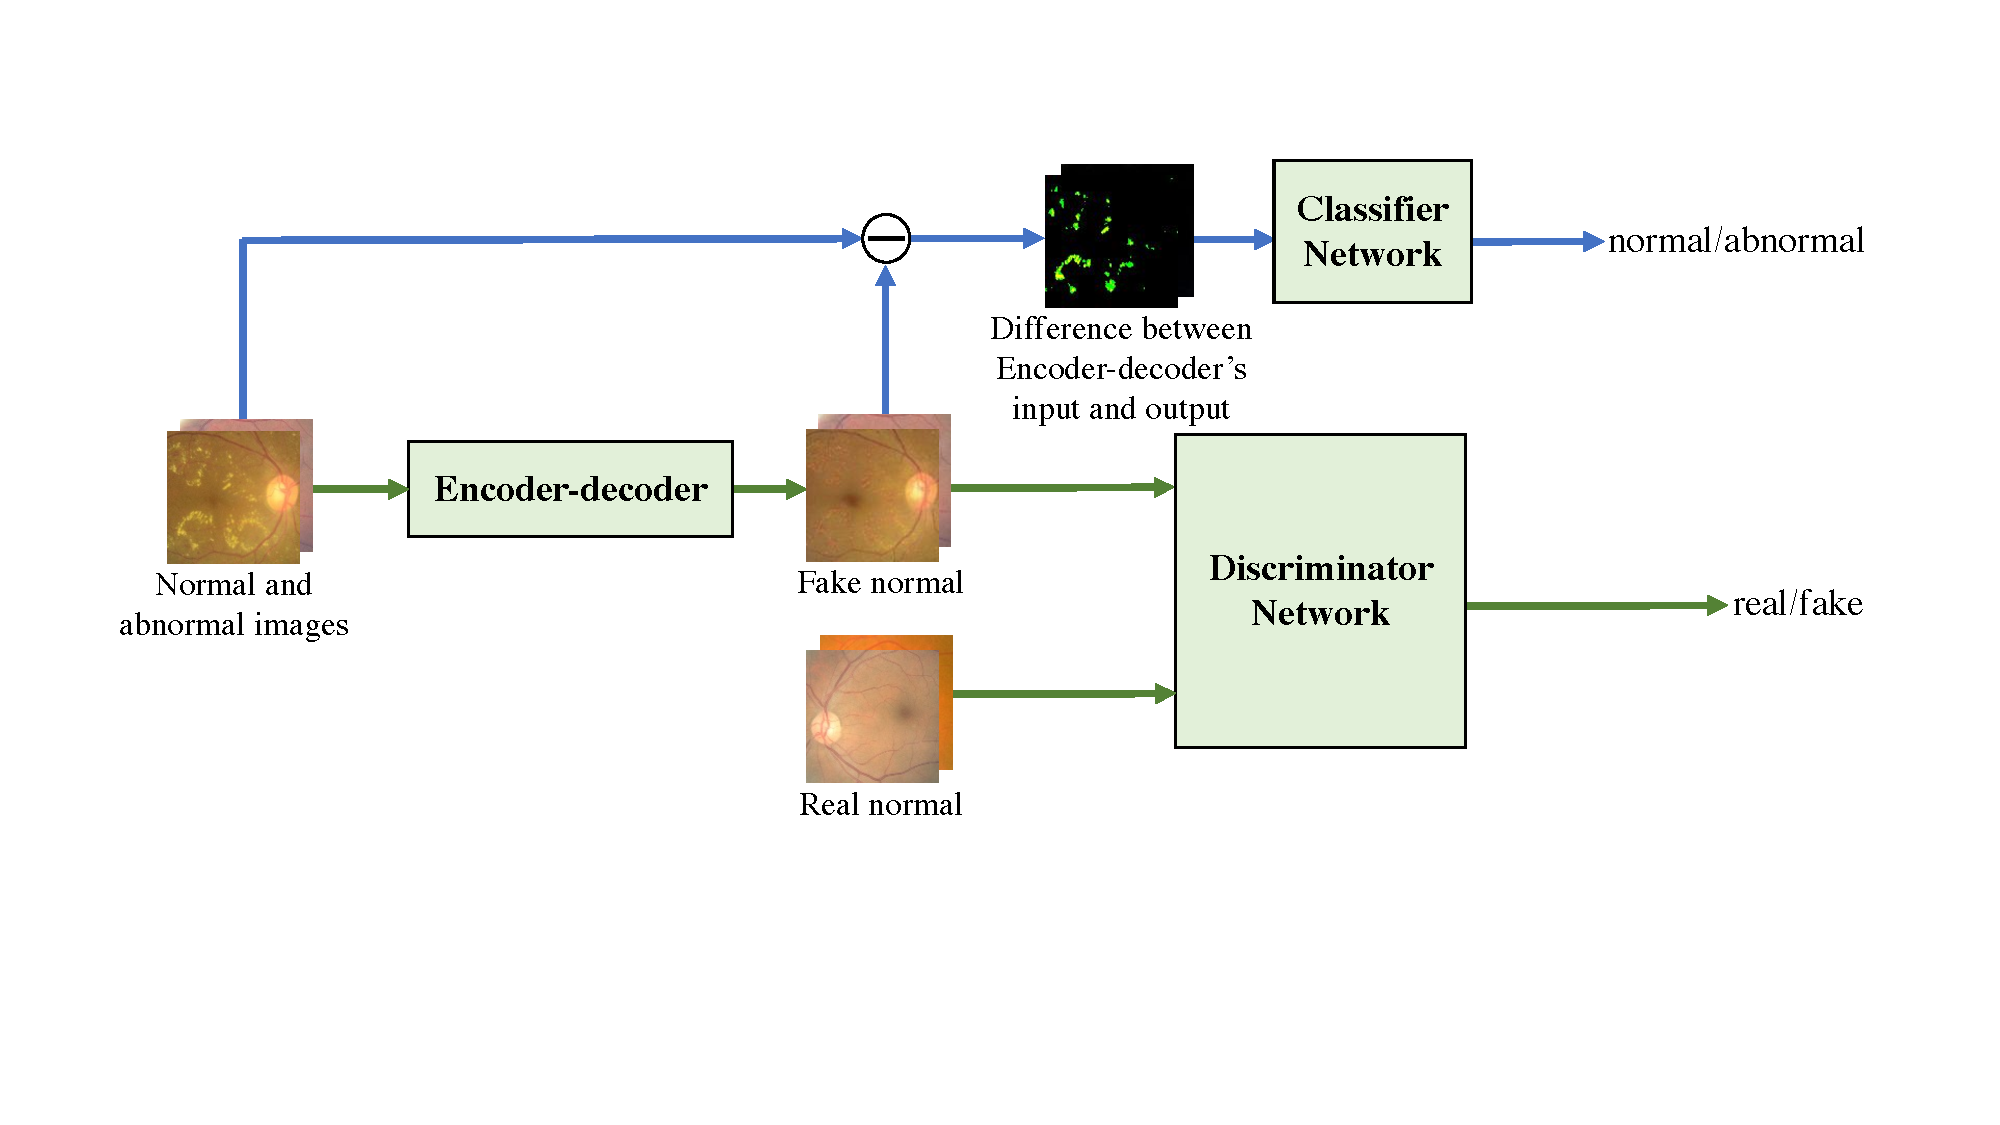
\includegraphics[width=1.0\textwidth]{figure/method.pdf}
	\caption[本文提出的疾病标记物定位网络]{本文提出的疾病标记物定位网络。} 
	\label{fig:our_model_architecture}
\end{figure}
在提出的体系结构中,编码器-解码器网络尝试从输入图像中删除任何潜在的生物标记,为异常的输入图像生成伪造的正常图像,或者在输入正常的情况下将输出图像与输入保持相同。通过从其输入中减去编码器-解码器的输出,可以轻松地对任何疾病标记物进行定位和分析。尽管可以仅使用正常图像来训练这种编码器-解码器,但这并没有利用现有的异常图像,因此不能直接学习生物标记特征以进行定位。取而代之的是,为了更有效地实现编码器-解码器的目标,在编码器-解码器的顶部添加了CNN分类器,其中输入是从其输入中减去编码器-解码器的输出,而期望的输出是原始输入图像的标签。为了准确地对图像进行分类,CNN分类器与编码器-解码器必须将异常图像与正常图像区分开。理想情况下,如果分类器的输入仅包含异常原始图像的生物标记,而对于正常图像则不包含任何生物标记(各处均为零),则分类器将更容易,也更准确地预测原始图像的类别。换句话说,训练更准确的分类器可以帮助编码器-解码器的输出保持正常区域,并从原始图像中移除疾病标记物,从而使分类器的输入仅包含疾病标记物的信号。

但是,分类器可能会帮助仅从原始输入图像中定位部分生物标记。这是因为定位来自原始异常图像的部分生物标记信号(以及定位来自正常图像的信号很少)足以使分类器轻松区分正常图像和异常图像。在这种情况下,编码器-解码器输出仍将包含一些生物标记。为了进一步帮助编码器-解码器从原始(异常)图像中删除潜在的生物标记,添加了一个判别器来判断编码器-解码器的输出是否看起来像真实的正常图像。 通过强制编码器-解码器的输出看起来更像正常图像,判别器帮助编码器-解码器从原始图像中去除尽可能多的生物标记信号。

显然,编码器-解码器和判别器一起形成了生成对抗网络。读者可能会认为,在架构中没有分类器组件的生成对抗网络本身足以帮助编码器-解码器从图像中删除潜在的生物标记。但是,生成对抗网络本身可能会提供过多帮助,以至于尽管编码解码器生成的图像过于正常,但与输入相比,编码器解码器输出的正常区域也可能会发生变化。在这种情况下,编码器-解码器的输出与其输入(即分类器的输入)相减会同时包含正常信号和生物标记信号,这又使分类器将异常图像与正常图像区分开来相对较困难。这意味着分类器和判别器应该一起工作以帮助编码器-解码器去除潜在的生物标记,即判别器帮助编码器-解码器输出正常图像,而分类器帮助编码器-解码器仅改变生物标记区域以生成正常输出。在实验也已经证实了这一点(参见第\ref{sec:experiments}相关章节)。

\subsection{编码器-解码器模块}\label{subsec:encoder_decoder_model}
\ref{subsec:model_architecture}小节中阐述了整体模型及各个子模块各自的作用,接下来进行子模块的介绍。本文决定在U-Net的基础上进行微调得到编码器-解码器,进而将U-Net迁移到本任务上来。原因主要有以下三点:

1)近些年来,U-Net在医学影像分析领域应用越来越广泛,无论是在处理医学分割上~\cite{oktay2018attention, dong2017automatic, zhang2018ct},还是在把U-Net当做生成器与其他判别器来组成生成对抗网络~\cite{Han2018SpineGANSS}上,U-Net都表现不俗、性能出色。

2)在疾病标记物的精确定位任务中,只需要极少像素强度发生改变,而其他绝大部分像素都需要较好的重建出来,而U-Net的跨层结构能够很好的将编码阶段的特征图融合到解码阶段,有利于图像尤其是具有丰富细节纹理的图像的重建。
%比如,眼底图像(见图\ref{fig:biomarker_localization_example})。

3)U-Net是全卷积网络的一种,可允许任意尺寸大小的图像输入,这增加了输入图像尺寸大小的灵活,上采样的倍数也可由U-Net的深度灵活控制。另外,由于跨层的存在,使得梯度回传比较容易,不容易出现梯度消失情况。

因此,本文选用U-Net为基本结构,将U-Net迁移到本文任务上来。与原始U-Net相比,本文编码器-解码器在模型结构上最终做了如下两点调整:

1)在编码阶段,为了减少在下采样过程中造成的信息丢失,本文采用的编码器-解码器中使用卷积(卷积核大小为$3\times 3$,步长为2)代替最大池化层。相应地,在解码阶段,编码器-解码器中使用反卷积(卷积核大小为$2\times 2$,步长为2)代替上采样操作。

2)由于编码器-解码器的输入图像经过预处理之后的范围为$[-1,1]$,在解码阶段的最后一个$1\times 1$卷积之后,编码器-解码器使用Tanh激活函数替代了Sigmod激活函数。

经过以上微调后,编码器-解码器的模型结构如图\ref{fig:auto_encoder_architecture}所示,图中输入图像尺寸为$128\times 128$,网络下采样次数为5。可以看出,编码器-解码器是以U-Net为骨架,编码阶段和解码阶段在网络结构上仍呈现“U”形。在编码阶段,随着深度的增加,特征图尺寸逐步减小,特征图数量或者说卷积核数量逐渐增加,直到到达最底层。与编码阶段相反,解码阶段随着深度的较少,特征图尺寸逐步增大,特征图通道数或者卷积核数量逐渐减小,同时来自编码阶段的特征不断通过跨层被融合到解码阶段的高层特征中,直到到达最顶层,随后经过一个卷积核大小为$1\times 1$、步长为$1$的卷积层,将特征图通道数降低至和输入图像一致,最后特征图经过Tanh激活函数作为网络输出。不难发现,编码器-解码器实际上通过编码器阶段和解码阶段完成了对输入图像的重建过程,保证了输入维度和输出维度相同。CNN分类器和判别器一起帮助本来无监督的编码器-解码器在此过程中去除图像中的疾病标记物。
\begin{figure}[h]
	\centering
	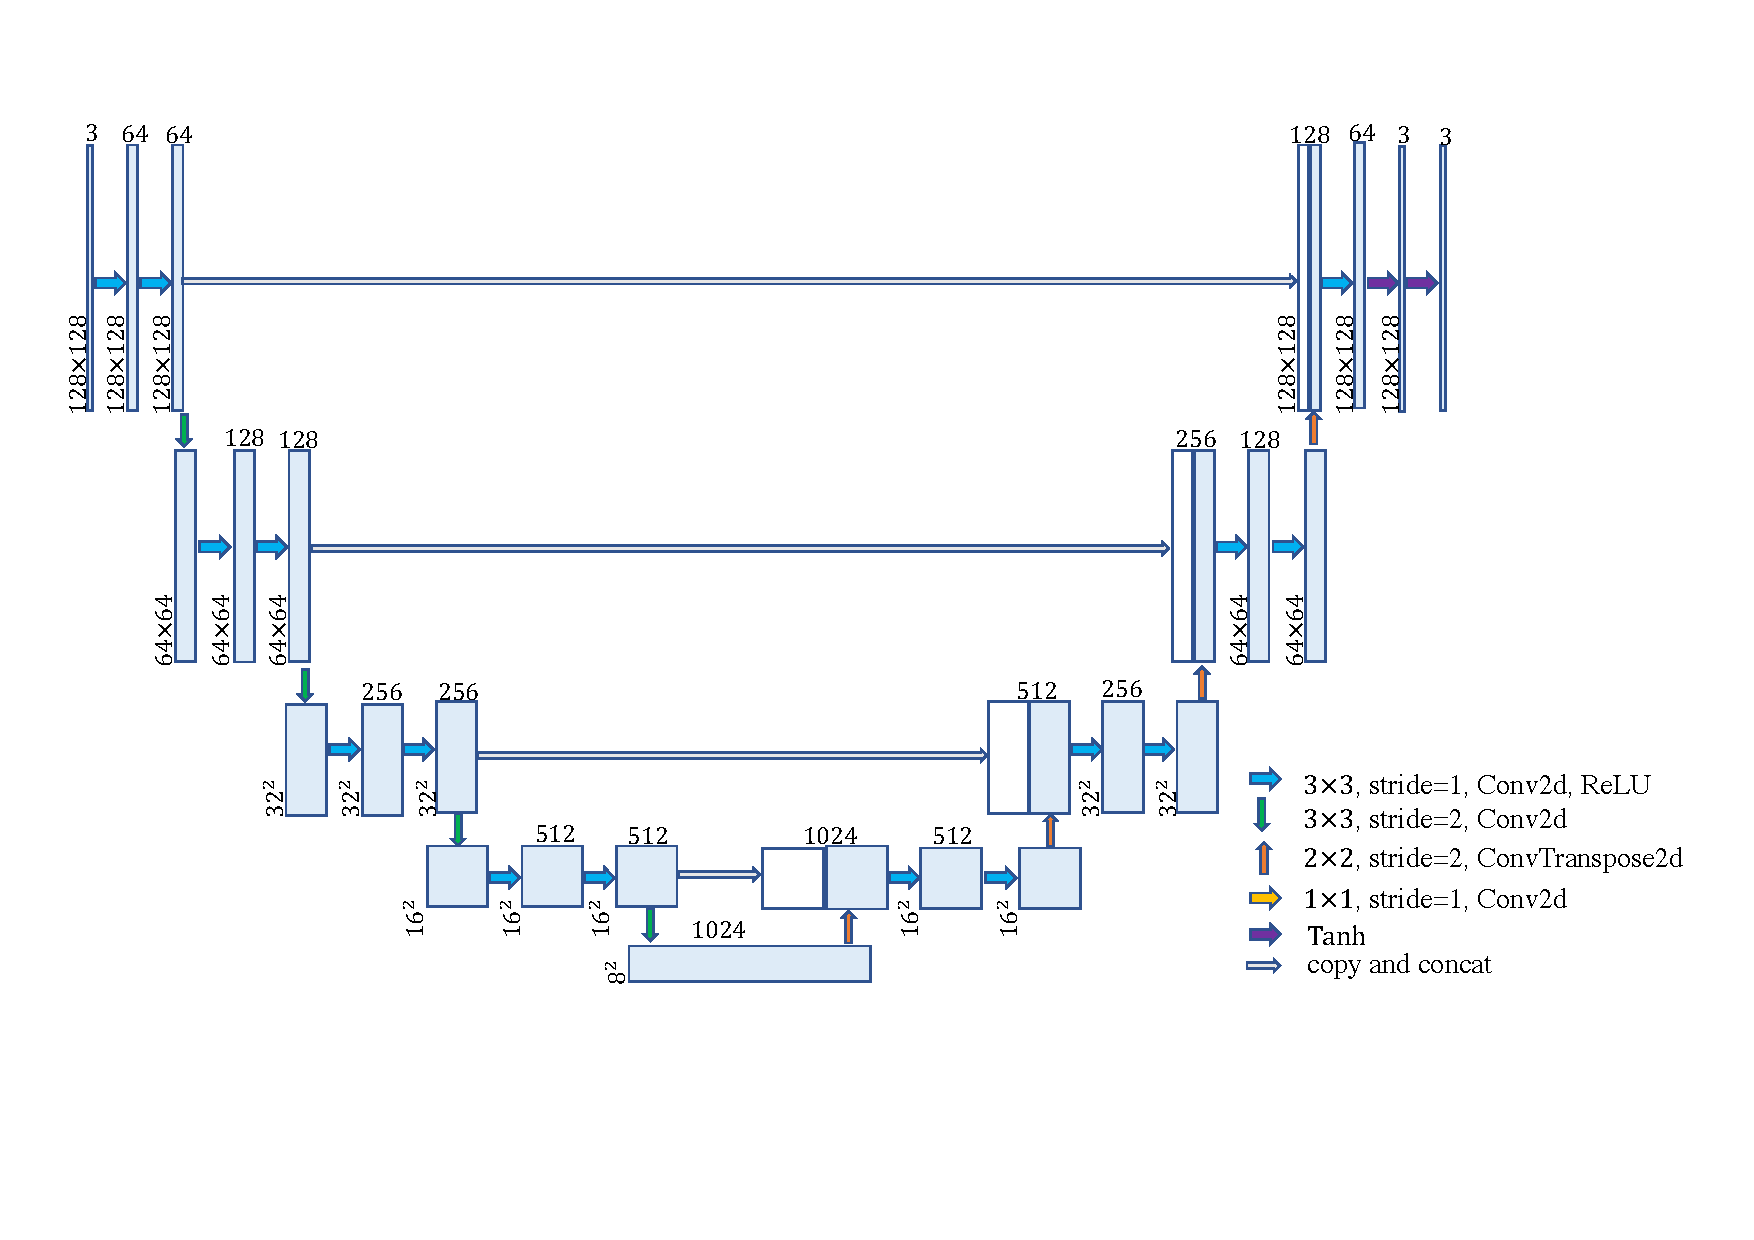
\includegraphics[width=1.0\textwidth]{figure/auto_encoder_architecture}
	\caption[本文编码器-解码器模块]{本文编码器-解码器模块。}
	\label{fig:auto_encoder_architecture}
\end{figure}
\subsection{CNN分类器模块}\label{subsec:cnn_classifier_model}
CNN分类器主要考虑的问题是如何选择一个较为优秀的分类网络,最终CNN分类器选择ResNet~\cite{he2016deep}。一方面,ResNet系列网络具有良好的特性。而编码器-解码器深度也较深,采用ResNet网络有利用避免梯度消失。另一方面,ResNet网络相对于VGG~\cite{simonyan2014very}等网络,参数量较少,计算开销较小。而相对于DenseNet~\cite{huang2017densely}、Inception~\cite{Szegedy2015RethinkingTI}等网络,ResNet模型结构较为简单,易于理解。CNN分类器的模型结构如图\ref{subfig:classifier_architecture}所示,可以发现,CNN分类器与原始ResNet-18相比没有作出较大改变,大部分卷积层(除跨层外)之后都会接上BatchNormalization层和ReLU激活函数,只是用$3\times 3$卷积层代替了原始$7\times 7$卷积层。这是因为原始ResNet-18的输入图像尺寸大小为$224\times 224$,而本文CNN分类器的输入图像尺寸大小为$128\times 128$。对于ResNet-18中的跨层连接,如果输入维度和输出维度相同,则直接相加(图\ref{subfig:classifier_architecture}中橘黄色折线);如果输入维度和输出维度不一样,本文使用卷积核大小为$1\times 1$、步长为$2$的卷积层将输入的尺寸大小减半(\ref{subfig:classifier_architecture}中蓝色折线),同时将卷积核数量加倍。为了在跨层中保持尽量避免梯度消失问题和提高训练速度,本文同样在该卷积层后接上BatchNormalization层。最后一层将经过全局均值池化层的特征图送入输出维度为$1$的全连接层(处理二分类问题)。

%由于ResNet-18中利用,对于图\ref{subfig:classifier_architecture}中的蓝色折线表示的跨层结构具有将输入尺寸减半的效果,这。
%\begin{figure}[h]
%	\centering
%	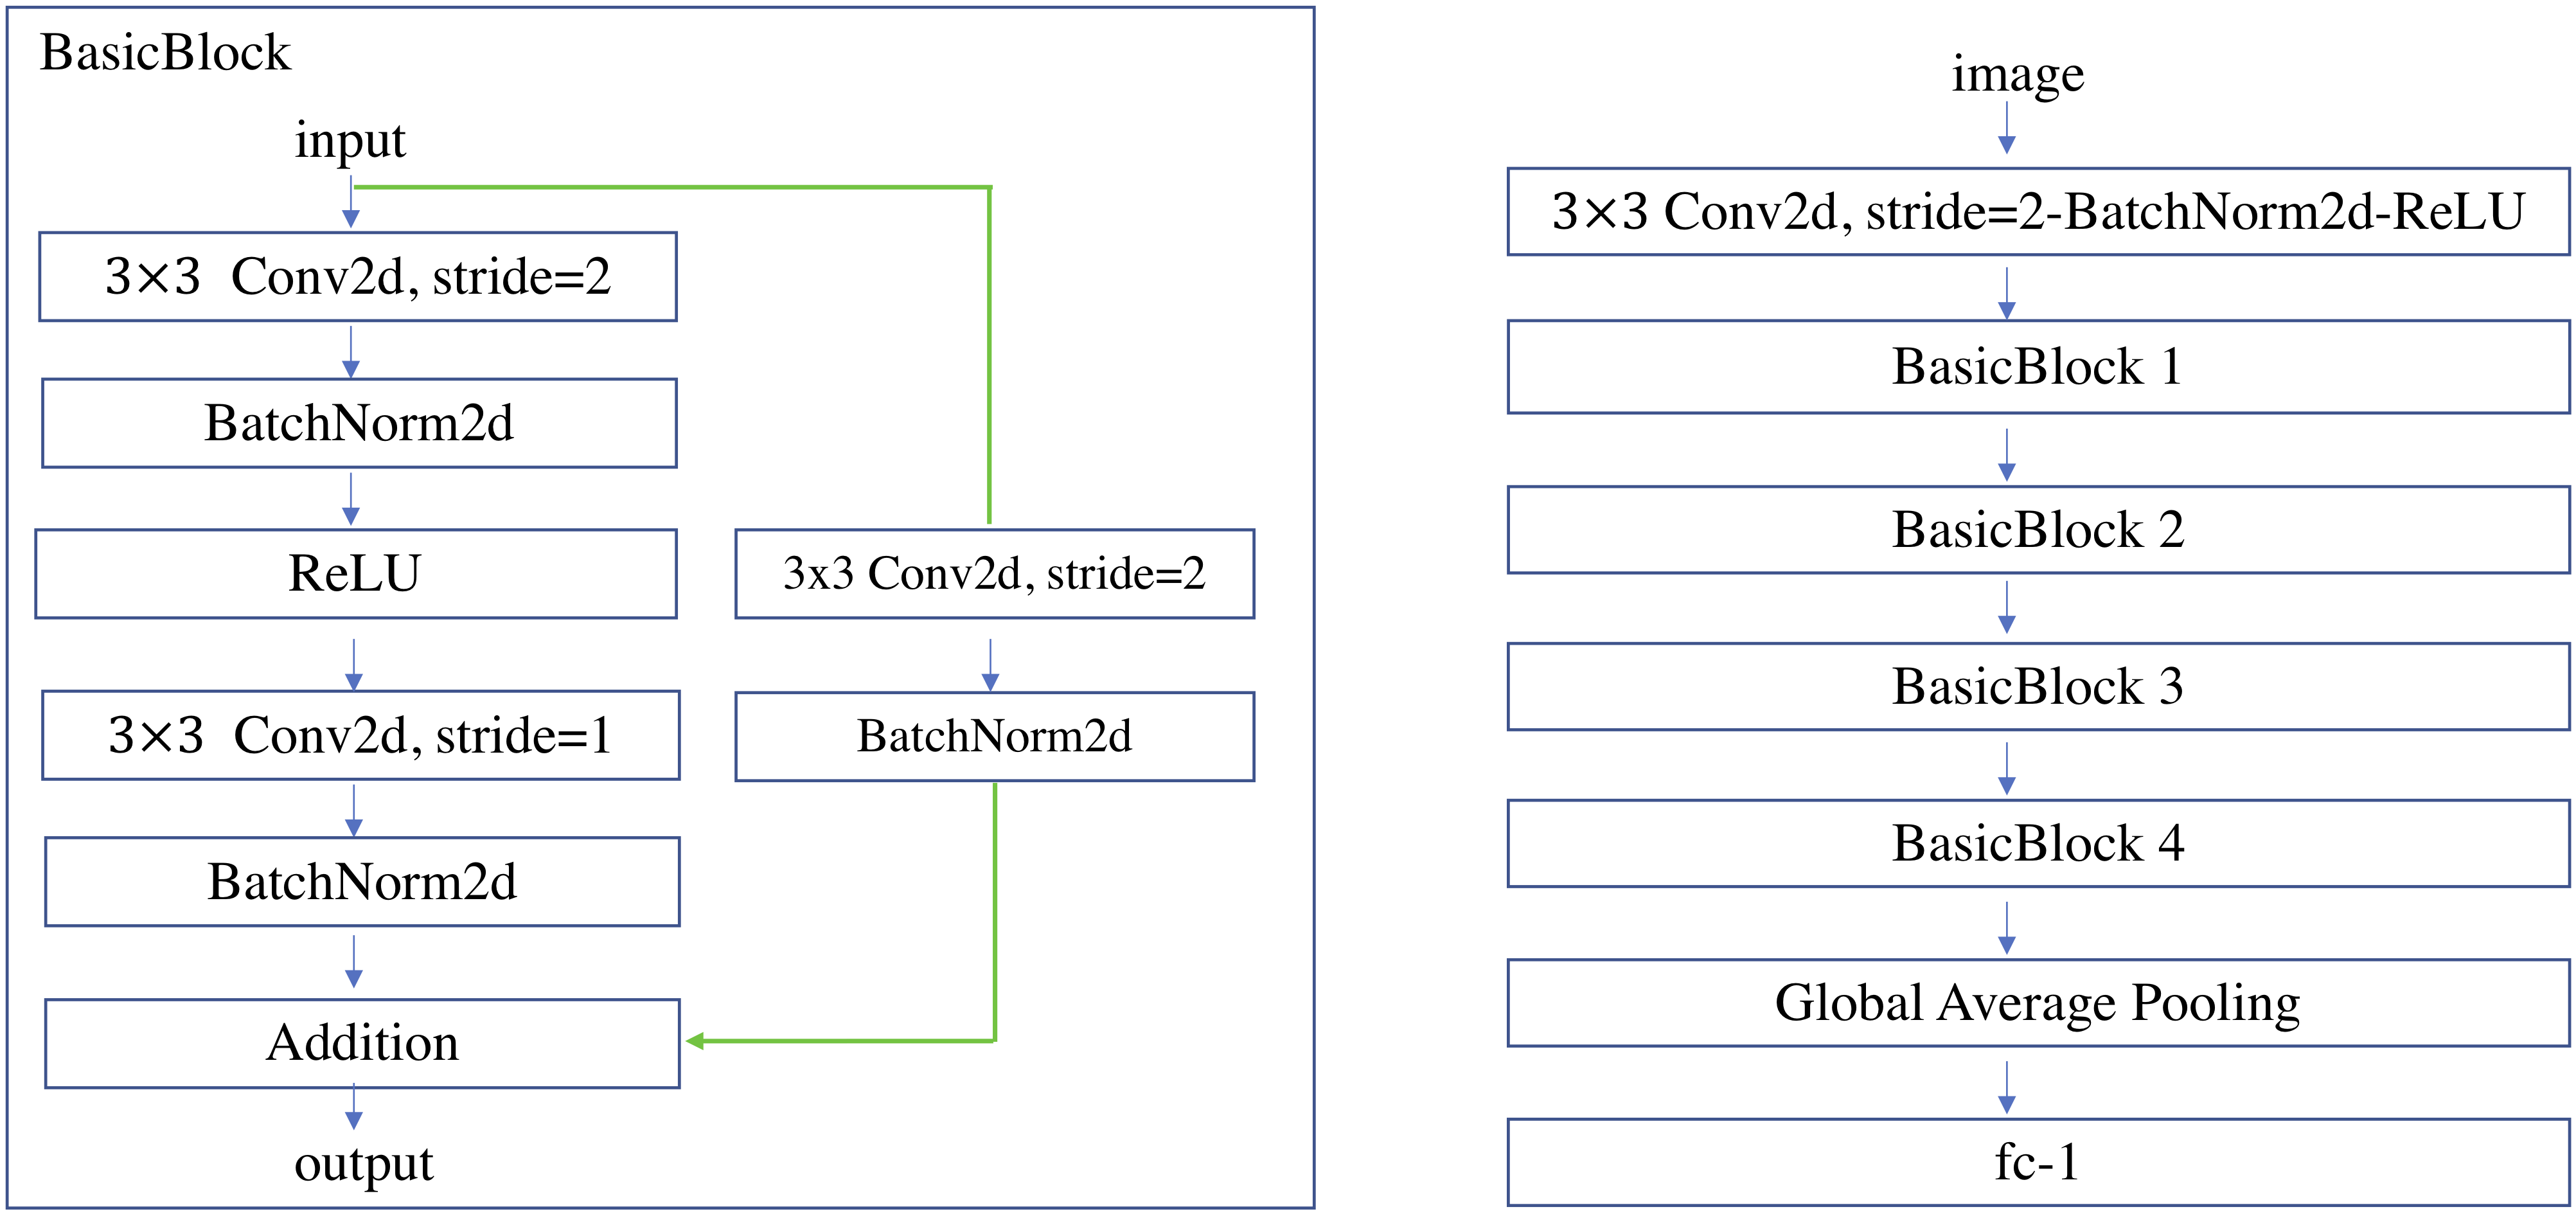
\includegraphics[width=1.0\textwidth]{figure/classifier_architecture.png}
%	\caption[本文CNN分类器模块]{本文CNN分类器模块。}
%	\label{fig:classifier_architecture}
%\end{figure}
\begin{figure}[h!]
	\centering
	\begin{subfigure}{0.3\textwidth}
		\centering
		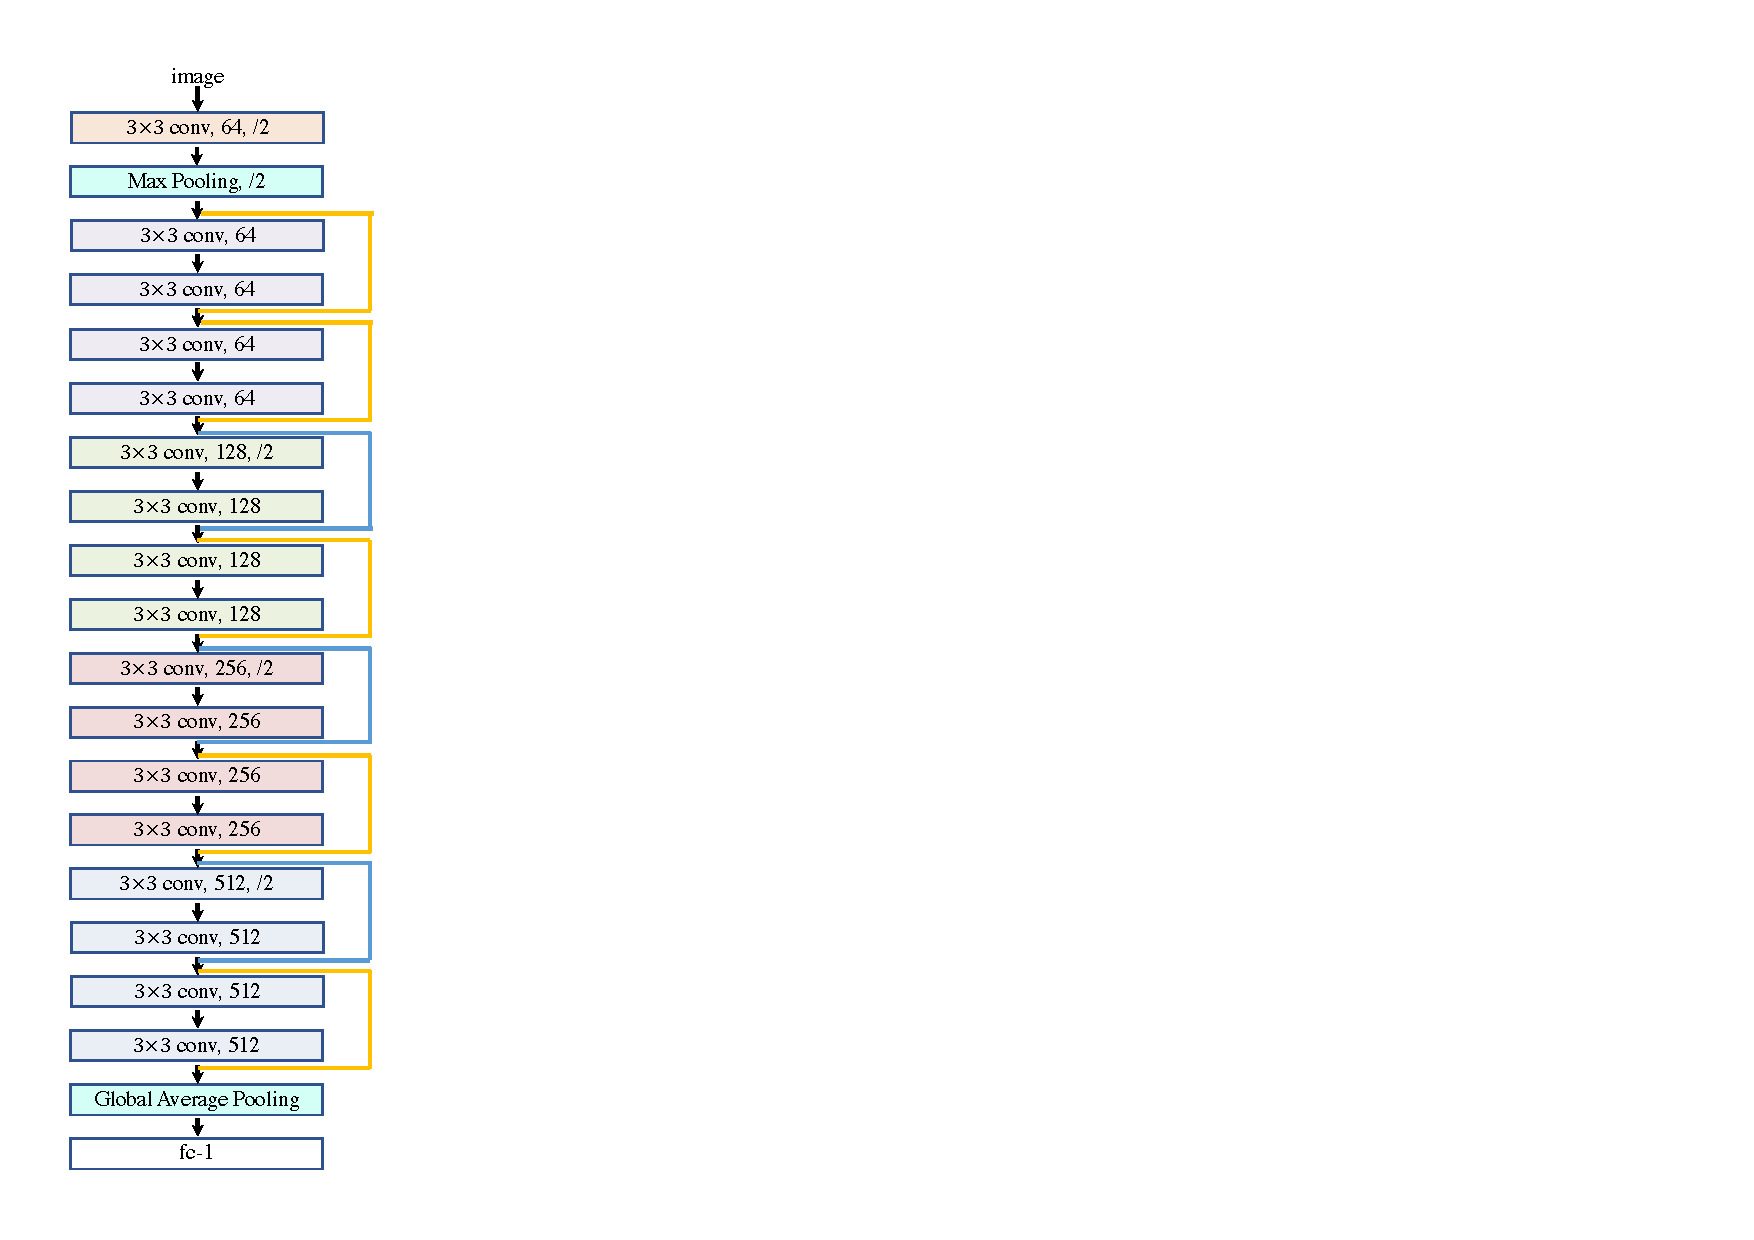
\includegraphics[width=1.0\textwidth]{figure/classifier_architecture.pdf}
		\caption{本文CNN分类器模块。}
		\label{subfig:classifier_architecture}
	\end{subfigure}
	\qquad\qquad\qquad\qquad
	\begin{subfigure}{0.348\textwidth}
		\centering
		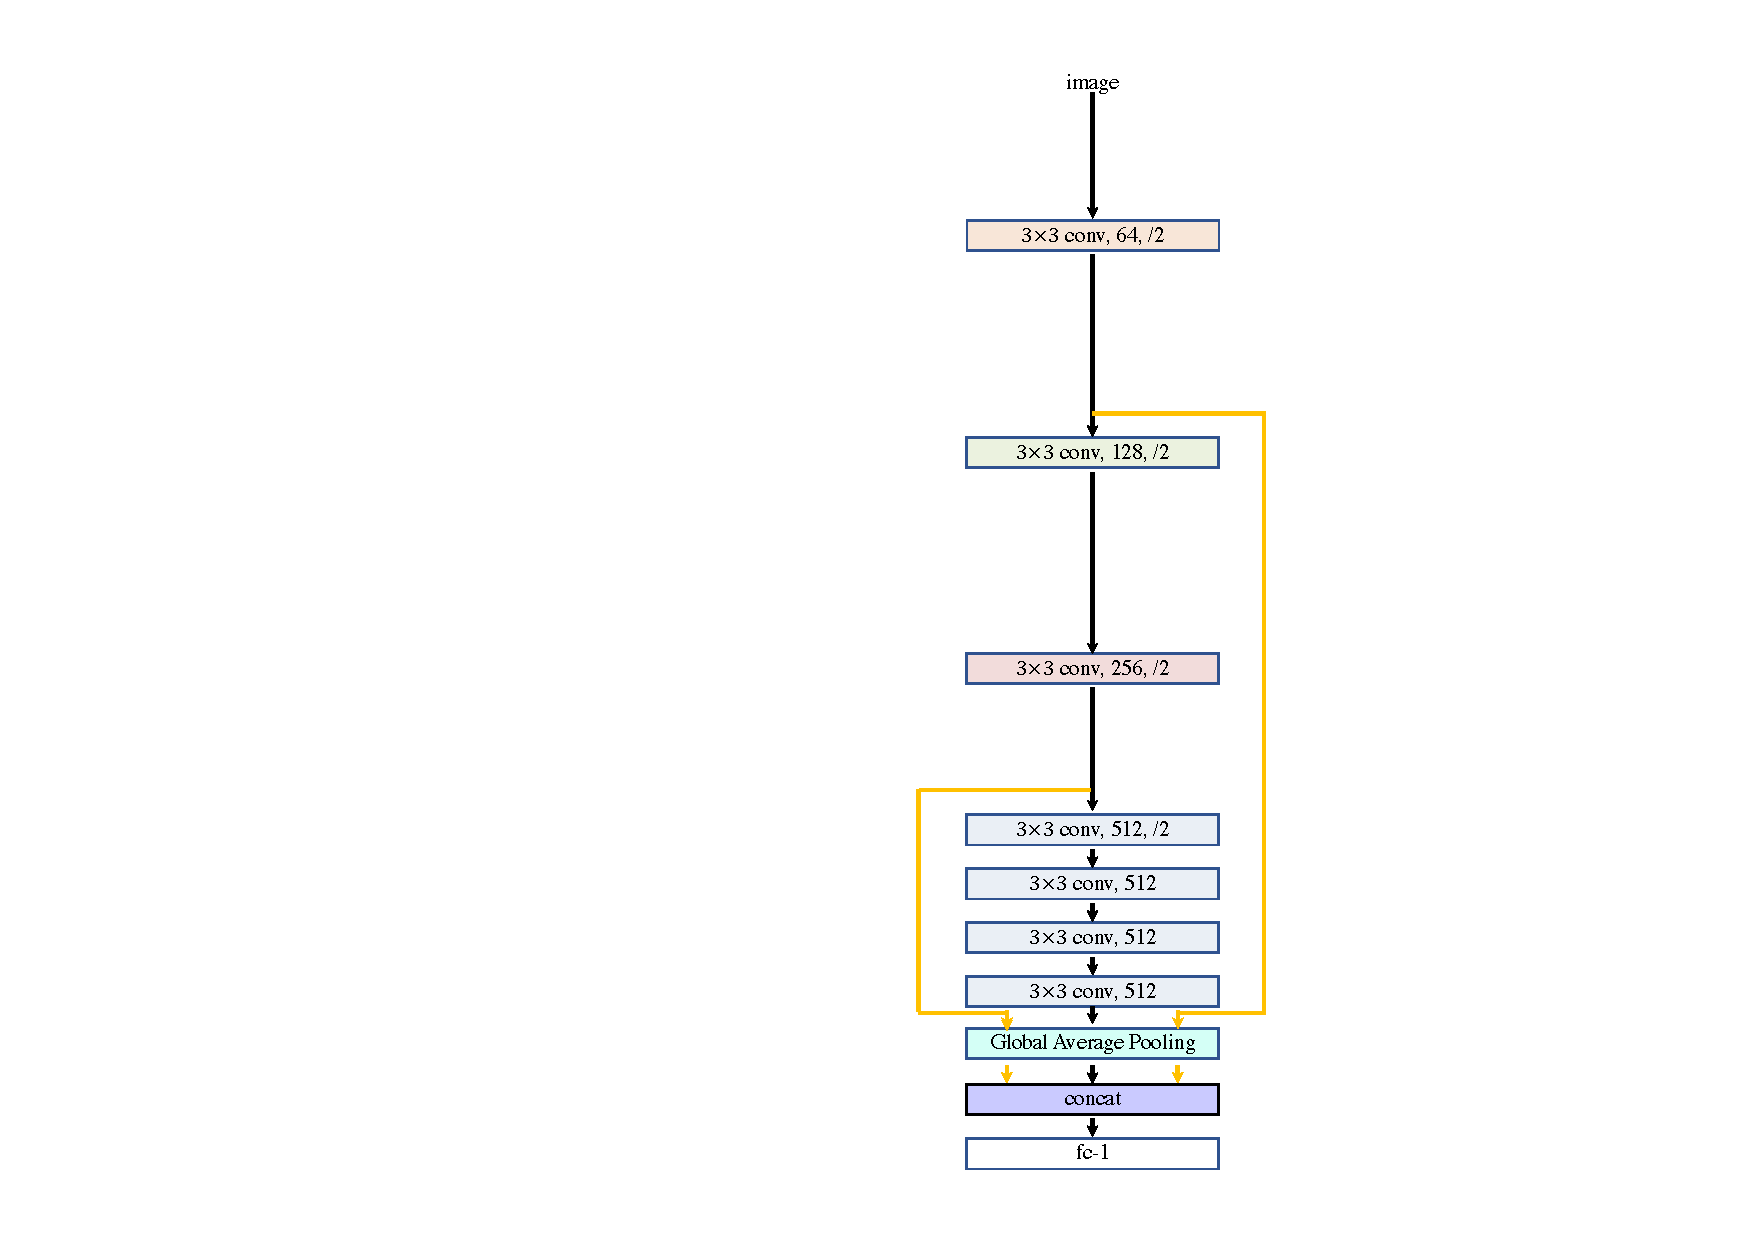
\includegraphics[width=1.0\textwidth]{figure/discrimintor_architecture.pdf}
		\caption{本文判别器模块。}
		\label{subfig:discrimintor_architecture}
	\end{subfigure}
	\caption[本文CNN分类器模块和判别器模块网络结构图]{本文CNN分类器模块和判别器模块网络结构图。CNN分类器网络和判别器网络的输入图像尺寸大小均为$128\times 128$。子图\ref{subfig:classifier_architecture}和子图\ref{subfig:discrimintor_architecture}中的橘黄色折线均表示跨层连接,子图\ref{subfig:classifier_architecture}中的蓝色折线表示可将输入尺寸大小减半的跨层连接。}
	\label{mul_fig:classifier_and_discrimintor_architecture}
\end{figure}
%本文使用卷积核大小为$1\times 1$,步长为$2$的卷积层实现输入尺寸减半这一目的,该卷积层随后接上BatchNormalization层。
\subsection{判别器模块}\label{subsec:discrimintor_model}
本小节将详细介绍本文判别器的模型结构。如图\ref{subfig:discrimintor_architecture}所示,判别器模块基本单元由卷积层(卷积核大小为$3\times 3$)、BatchNormalization层~\cite{ioffe2015batch}和Leaky ReLU激活函数~\cite{maas2013rectifier}(负斜率为0.2)组成。如图\ref{subfig:discrimintor_architecture},对于前$4$个卷积层,本文采用步长为2的$3\times 3$卷积层达到下采样的目的,与此同时,随着特征图尺寸不断减小,卷积核的数量也以$2$倍关系增长(卷积核数量基数为64);对于第$5-7$个卷积层,卷积操作的步长为$1$,特征图尺寸不会发生变化,同时卷积核数量也不发生改变。最后,第一个下采样卷积层的特征图输出、最后一个下采样卷积层的特征图输出以及最后一个卷积层的特征图输出在经过全局均值池化层之后再进行拼接操作(图中concat操作),来融合低分辨率但语义强的特征(最后一个卷积层的特征图输出)和高分辨率但语义弱的特征(第一个下采样卷积层的特征图输出和最后一个下采样卷积层的特征图输出),最后将特征图送入输出维度为$1$全连接层。不难发现,判别器网络结构由下采样卷积层层数和卷积层总层数共同决定。在上文提到的诸多GAN中,训练WGAN-GP时梯度相对比较稳定,不易发生梯度消失,损失函数对训练过程也有指示作用,故本文选用WGAN-GP~\cite{gulrajani2017improved},此时判别器不再是二分类器,而是去拟合Wasserstein-1距离的回归器。
%故最后一层全连接层之后也没有Sigmoid激活函数。
%\begin{figure}[h]
%	\centering
%	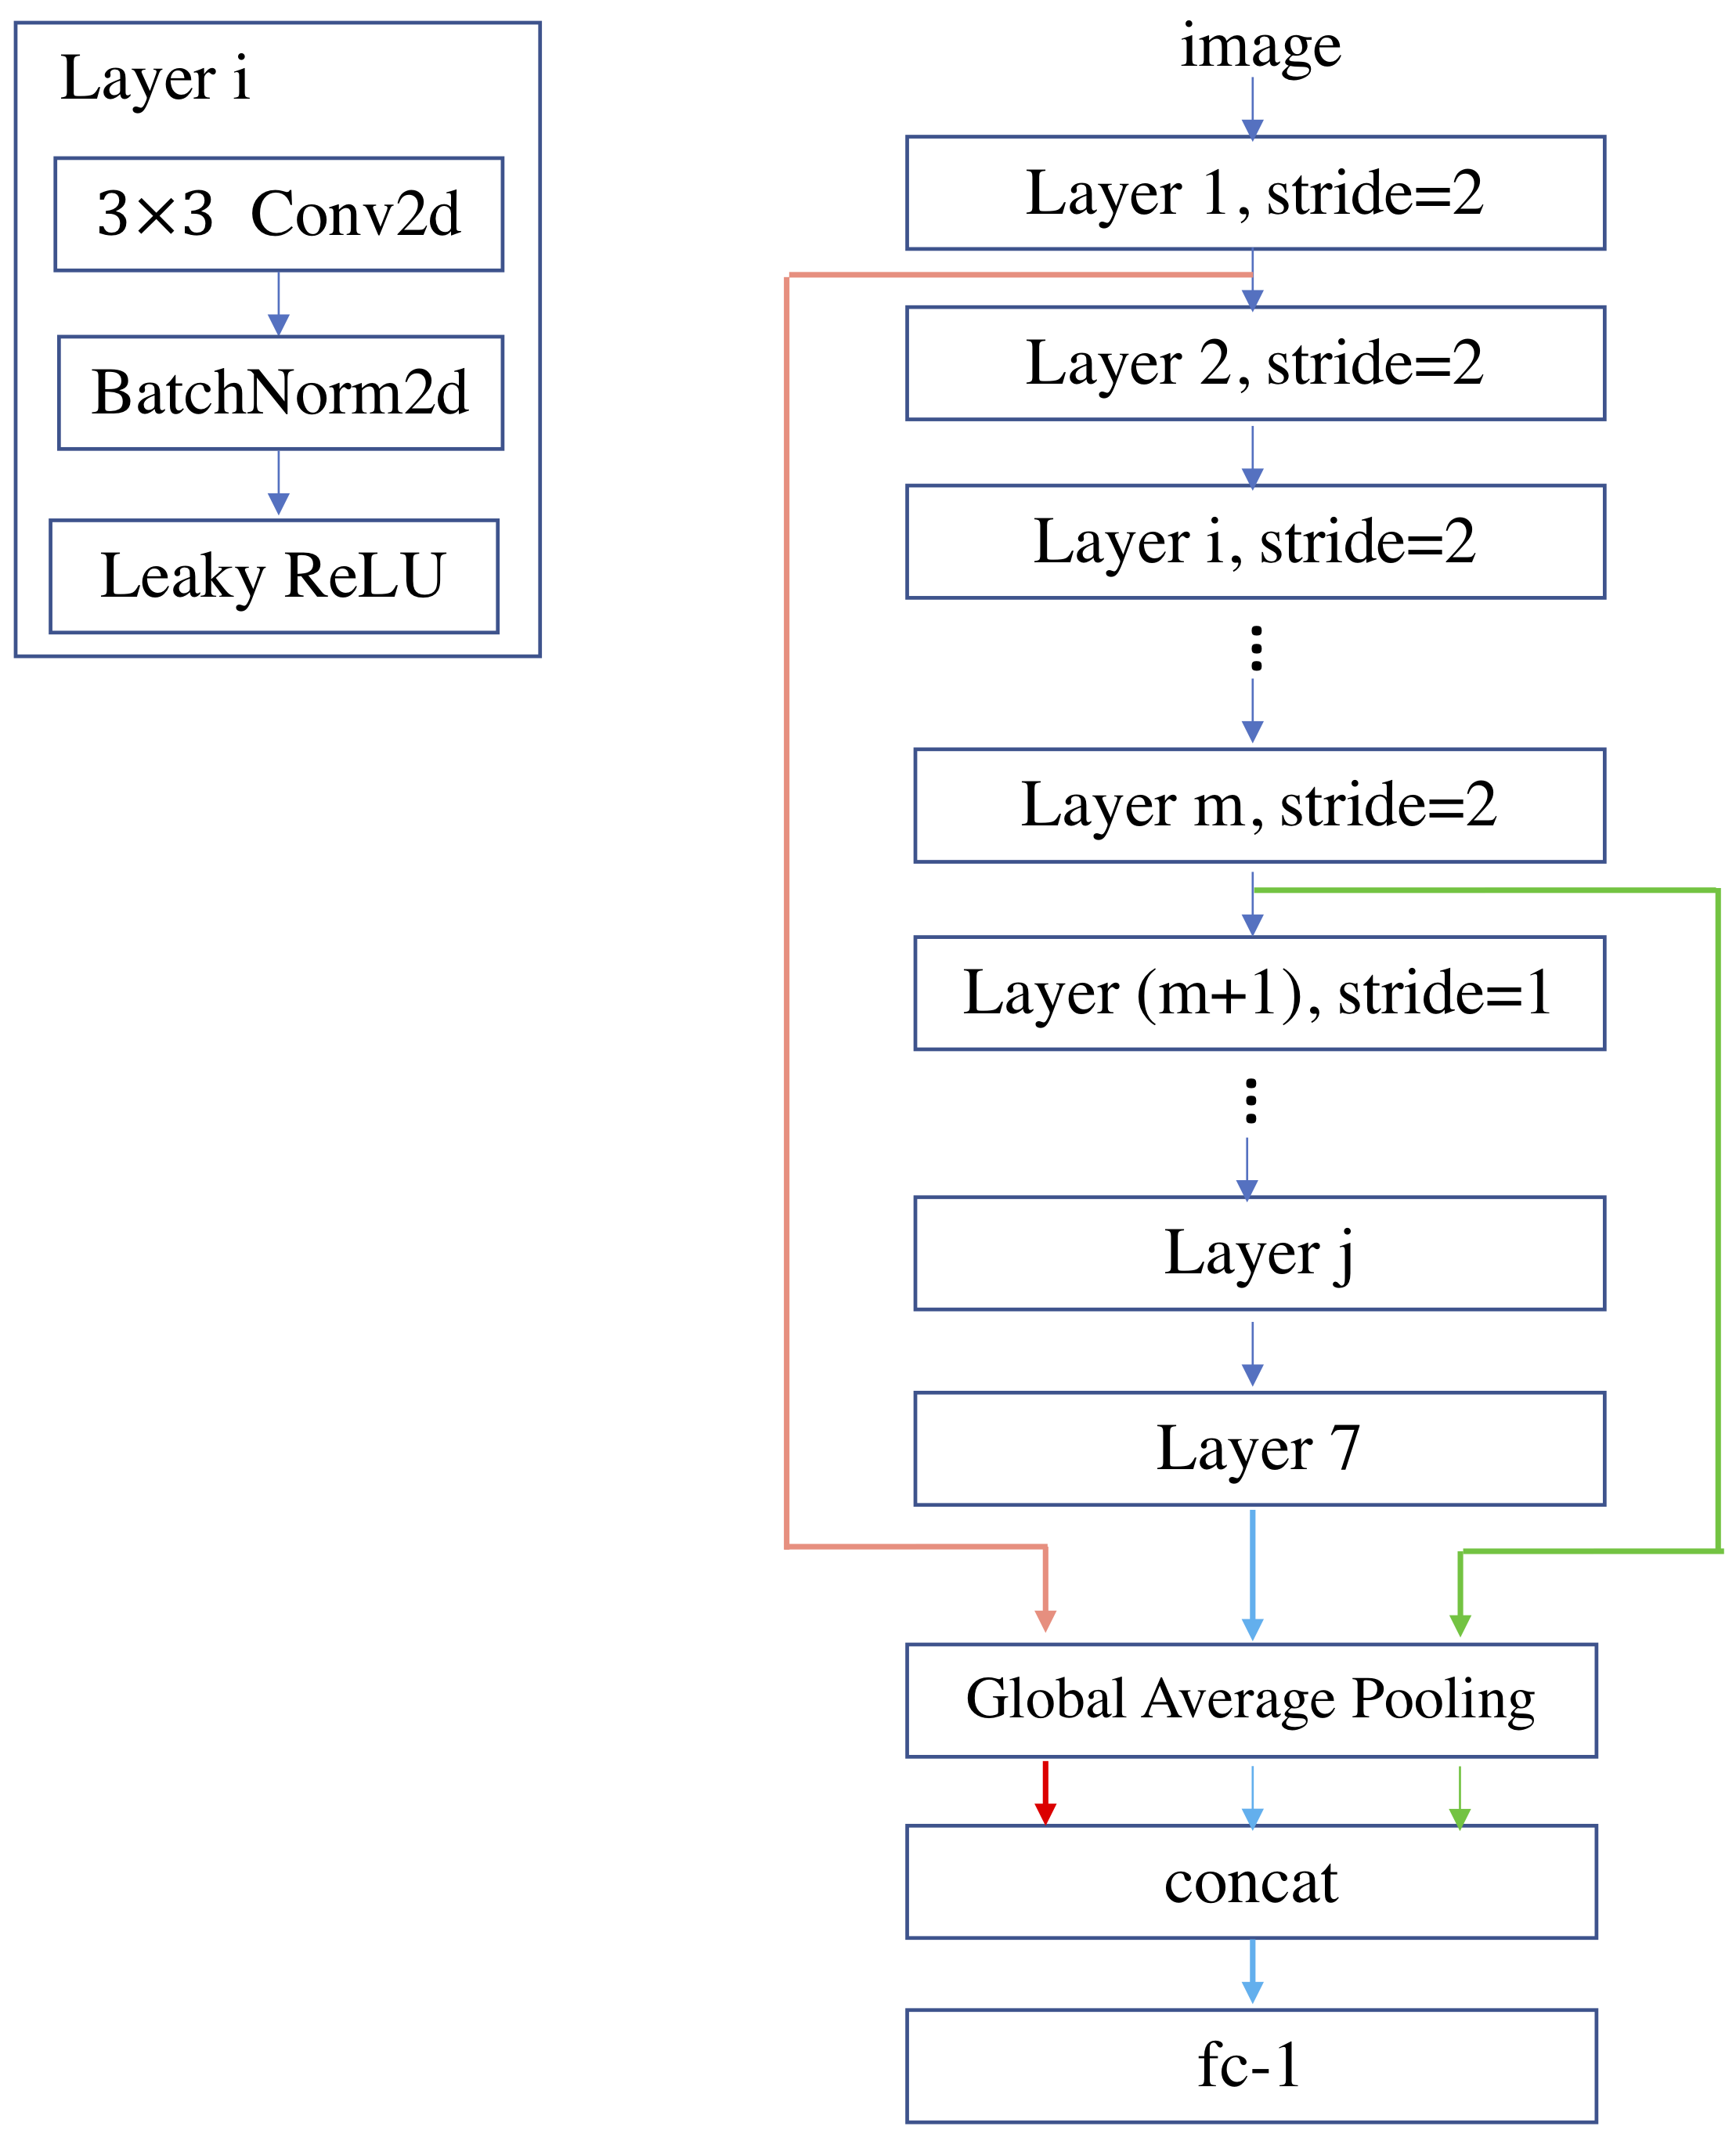
\includegraphics[width=1.0\textwidth]{figure/discrimintor_architecture.png}
%	\caption[本文判别器模块]{本文判别器模块。}
%	\label{fig:discrimintor_architecture}
%\end{figure}

本文参考了特征金字塔~\cite{lin2017feature},判别器模块和与普通GAN中的判别器相比,最主要的改动是增加了跨层结构。该结构通过从上而下的路径连接,来将低分辨率但语义强的特征和高分辨率但语义弱的特征结合起来,使得原图像中的丰富细节信息比如纹理信息都能被捕捉到。换句话说,就是使用内网倒特征金字塔(特征图尺寸从上到下依次减小)取代特征化图像倒金字塔(随着卷积的堆叠,特征图尺寸依然是从上到下依次减小),且没有牺牲表示能力,速度和内存。这种设计最初用于解决物体检测中小物体在连续特征图的下采样过程中容易被忽略的问题。由于浅层高分辨率但语义弱的特征中往往包含了小物体的信息,故可通过多尺度特征图的融合,可以将这些小物体的特征直接送到高层,与低分辨率但语义强的特征结合起来,使得各种大小不一的物体都能被CNN检测到。而医学影像中的疾病标记物也有这种特点,具体来说,疾病标记物的形状通常是不确定的,大小各异,并且数量往往不是一个,而是多个。因此,如果对这些大小不一的疾病标记物进行比较,也会发现有些疾病标记物属于大物体或者说大目标,而另外一些疾病标记物属于小物体或者说小目标,甚至还会存在一些人类甚至专业医生都难以察觉到的微小疾病标记物。也就说,这种在物体检测问题中出现的小物体难以发现的难题在医学影像领域的疾病标记物定位问题中不光存在,而且更加突出。这也是本文判别器模型中加入跨层结构的必要性所在。

\section{训练策略与损失函数}\label{sec:loss_func_training_stragies}
在\ref{sec:model_architecture_intro}小节中,本文介绍了本文提出方法的模型结构以及各个子模块(CNN分类器、判别器和编码器-解码器)所扮演的角色。本节内容将在此基础上介绍模型的训练策略(见\ref{subsec:traing_stragies}小节)以及损失函数(见\ref{subsec:loss_func}小节)。
\subsection{训练策略}\label{subsec:traing_stragies}
如\ref{subsec:model_architecture}所描述的那样,本文提出的网络模型中共有三个子模块:编码器-解码器、CNN分类器和判别器。根据\ref{sec:idea_thinking}小节描述的解决思路:编码器-解码器是一种无监督模型,本身并没有识别疾病标记物的能力,因此需要借助其他模块来指导编码器-解码器,使得编码器-解码器能够识别图像中的疾病标记物,进而通过编码阶段和解码阶段来去除输入图像上的疾病标记物,这也是模型结构中引入CNN分类器和判别器的原因。具体展开来讲,本文希望先让CNN分类器来完成分类任务来迫使编码器-解码器具有一定识别疾病标记物的能力,尽量去除疾病标记物。一旦CNN分类器出现疾病标记物去除不够彻底,仍有比较微小的、难以察觉的疾病标记物存在,这时便通过训练生成对抗网络来迫使编码器-解码器进一步完全去除疾病标记物,故本文将在第一步中训练CNN分类器,在第二步中训练GAN。综上所述,本文提出的两步训练策略如下:

1)固定判别器,更新编码器-解码器和CNN分类器(以下简称“第一步”):这一步将编码器-解码器和CNN分类器联合起来训练,更新编码器-解码器和CNN分类器的模型参数。这一步旨在让CNN分类器完成一个分类任务。训练结束后,希望CNN分类器能够尽量识别出疾病标记物,使得编码器-解码器能在异常图像输入情况下尽量去除异常图像中疾病标记物。注意此时判别器并未参与训练过程。

2)固定CNN分类器,更新编码器-解码器和判别器(以下简称“第二步”):第二步将编码器-解码器和判别器联合起来训练,旨在训练一个性能优异的生成对抗网络,其训练过程与GAN-GP一致,分为两个子步骤,按照先后顺序依次更新判别器(注意固定编码器-解码器)和编码器-解码器(注意固定判别器)。我们希望在上一步仍无法彻底疾病标记物(部分去除)的情况下,编码器-解码器在经过对抗学习(真实正常图像 vs. 编码器-解码器的输出图像)之后能进一步彻底去除图像中的疾病标记物,生成异常图像对应的“正常”图像。注意此时CNN分类器并未参与训练过程。

注意,默认每训练一批数据(Mini-batch)后上述两个步骤就会交替训练一次,这种频繁的交替训练可能会造成GAN在训练的过程中发生震荡,为避免这种问题,可以选择训练所有数据(Epoch)后再交替训练一次。为了让CNN分类器在初始化情况下就具备一定识别疾病标记物的能力,以期望在第一步中,CNN分类器能指导编码器-解码器尽量去除图像中的疾病标记物,可先将第一步连续训练多次或者利用预训练参数初始化CNN分类器。对于纹理结构比较丰富的医学图像(比如,眼底图像),可用梯度算子(比如,索贝尔算子\footnote{https://en.wikipedia.org/wiki/Sobel\_operator}和拉普拉斯算子\footnote{https://en.wikipedia.org/wiki/Laplace\_operator})检测边缘,以便于编码器-解码器能更加容易地重构这些复杂的纹理结构。

待本文提出的模型训练完成之后,疾病标记物的位置就可以通过编码器-解码器的输出与输入之差给出了。而输入图像的标签,则可以由CNN分类器给出。
%\begin{figure}[h]
%	\centering
%	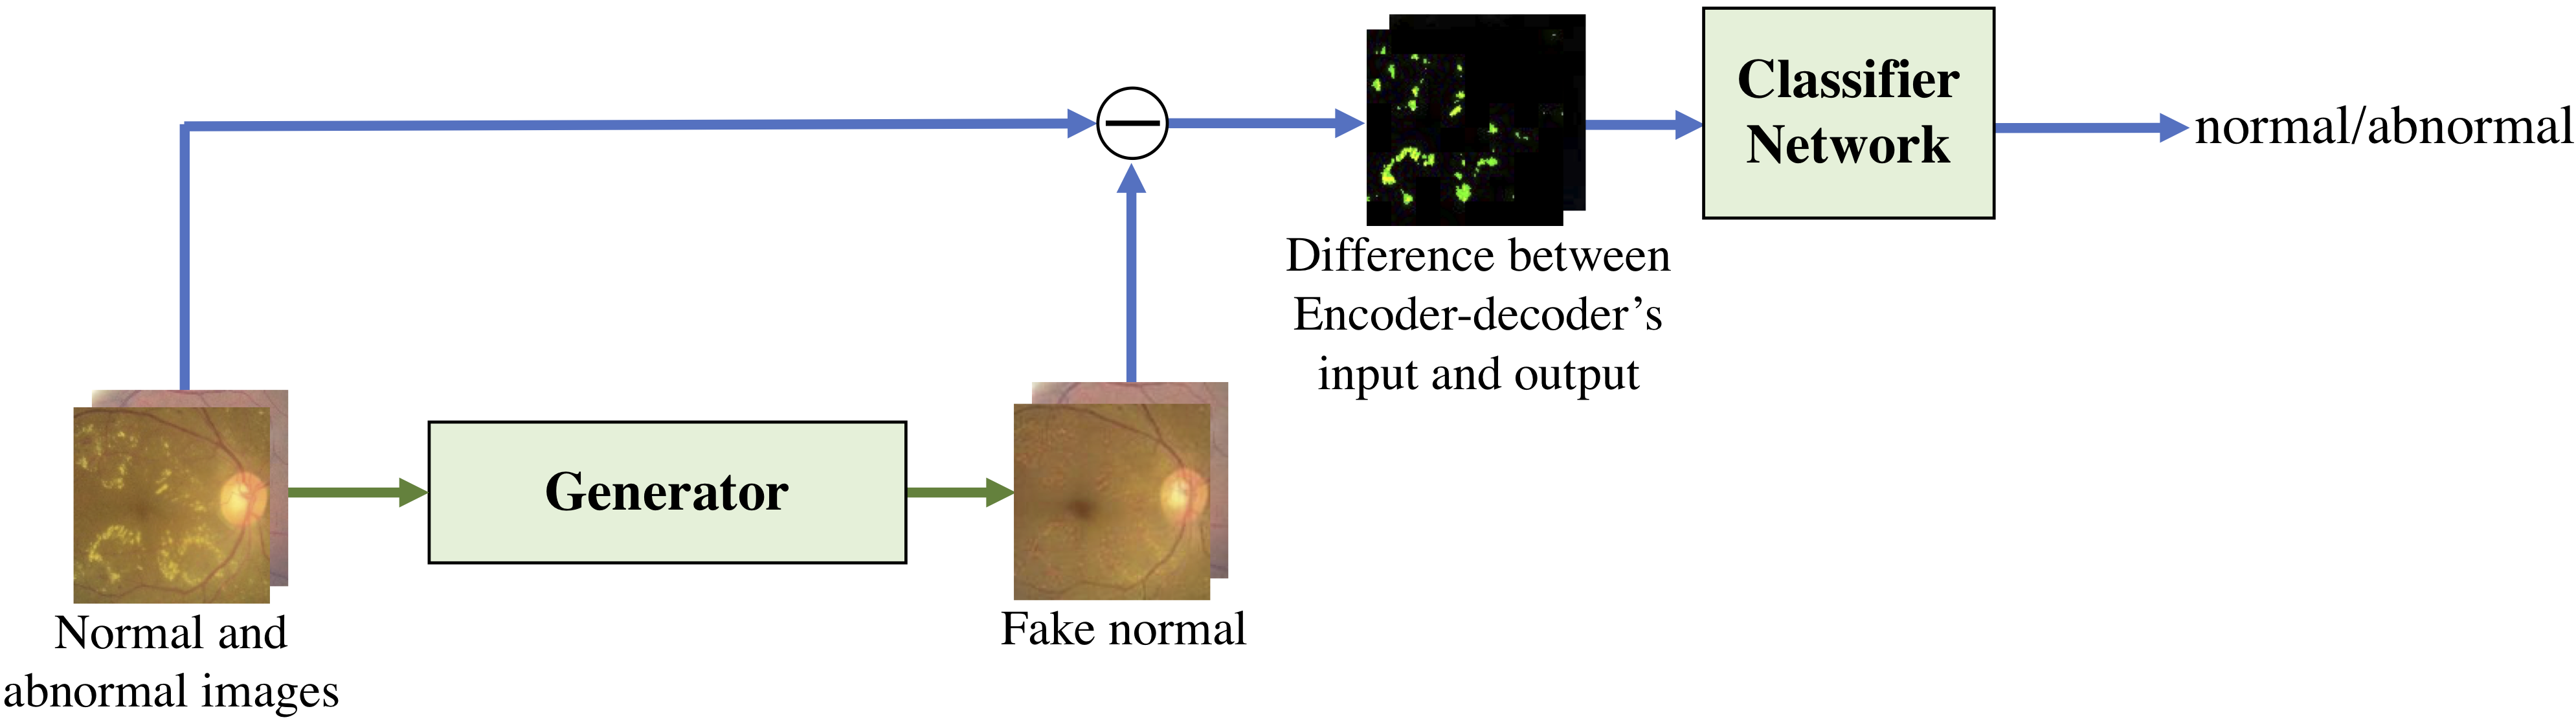
\includegraphics[width=1.0\textwidth]{figure/u_c_architecture.png}
%	\caption{同时训练编码器-解码器和CNN分类器的实际有效模型结构图。}
%	\label{fig:u_c_architecture}
%\end{figure}
%\vspace{-2cm}
%\begin{figure}[h]
%	\centering
%	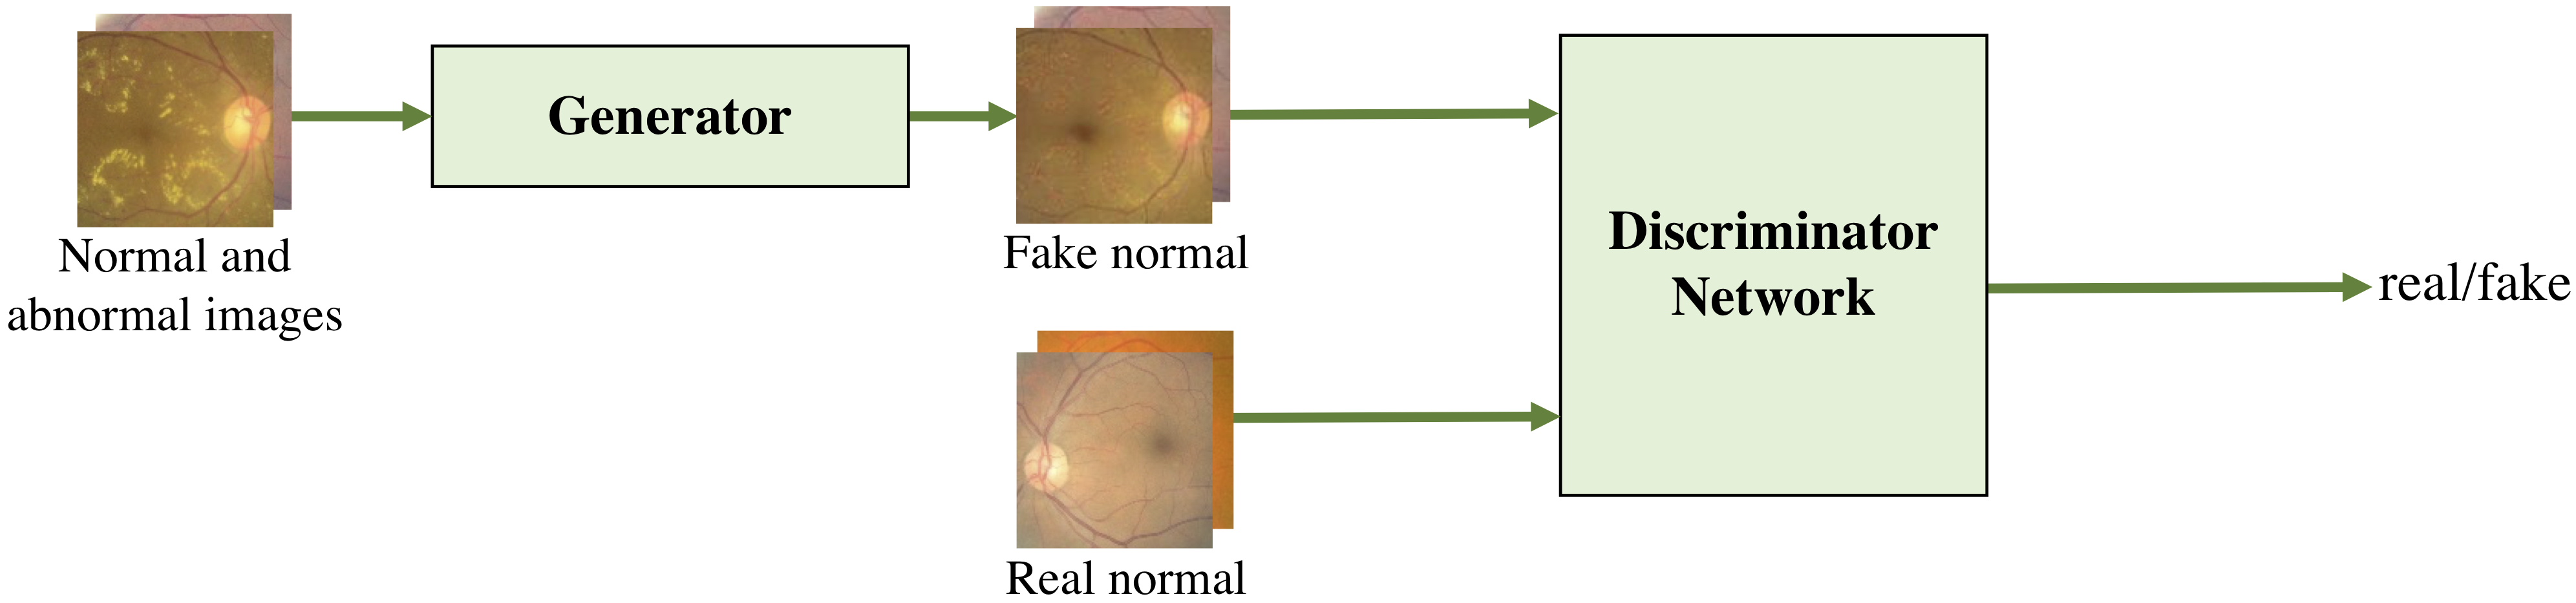
\includegraphics[width=1.0\textwidth]{figure/u_d_architecture.png}
%	\caption{同时训练编码器-解码器和判别器的实际有效模型结构图。}
%	\label{fig:u_d_architecture}
%\end{figure}
\subsection{损失函数}\label{subsec:loss_func}
接下来,本小节将介绍本文提出的模型在处理疾病标记物定位任务时的损失函数,不妨用$G$表示编码器-解码器,用$D$表示判别器,用$C$表示CNN分类器。设疾病标记物定位问题的损失函数为$\mathcal{L}$,本文将$\mathcal{L}$定义为:
\begin{equation}\label{equ:model_loss_func}
\mathcal{L}=\min _{G, C} \max _{D} \quad L_{GAN}(D, G)+\lambda_{1} L_{C E}(C, G)+\lambda_{2} L_{E D}(G).
\end{equation}
其中,$L_{GAN}(D,G)$表示生成对抗网络的损失函数(本文使用WGAN-GP),$L_{CE}(C, G)$表示CNN分类器的交叉熵损失函数,$L_{E D}(G)$是约束编码器-解码器的损失函数(本文使用L1损失函数),用于强调输入和输出之间的相似性,$\lambda{1}$和$\lambda_{2}$是两个超参数,用于平衡各个损失函数之间的权重。注意$L_{E D}(G)$这一项是不可缺少的,一旦缺少($\lambda_{2}=0$),在CNN分类器和判别器的指导下,编码器-解码器很可能在修改疾病标记物所在区域的同时还会修改正常区域,导致不可避免地出现假阳现象。

接下来,本文将给出每个步骤训练时的损失函数。根据等式\ref{equ:model_loss_func}和\ref{subsec:traing_stragies}小节中描述的训练策略,本文可进一步分别给出本文两步训练策略对应的损失函数。设第一步和第二步的损失函数分别为$L_1$和$L_2$,则第一步训练的损失函数$L_1$定义为:
\begin{equation}
\min_{G, C} \;\; L_{1}=\lambda_1 L_{CE}(C,G) + \lambda_2 L_{ED}(G).
\end{equation}
%设正常图像数据分布为$\ve{x}\sim \text{p}_{\text{n}}(\ve{x})$,异常图像数据分布为$\ve{z}\sim \text{p}_{\text{l}}(\ve{z})$,包括正常图像和异常图像在内的所有图像数据分布为$\ve{y}\sim \text{p}_{\text{all}}(\ve{y})$,分布$\text{p}_{\text{all}}$的随机取样$\ve{y}$对应的图像标签为$\ve{l}$,分布。设第一步的损失函数为$L(\ve{x};\vv{\theta})$,则第一步训练的目标是最小化损失函数$L(\ve{x};\vv{\theta})$:
%\begin{equation}
%L(\ve{x};\vv{\theta}) = \lambda_{1} %L_{CE}(G(\ve{x};\vv{\theta})-\ve{x},\ve{l}) + %\lambda_{2}L_{ED}(G(\ve{x};\vv{\theta}), \ve{x}).
%\end{equation}
在第二步中,编码器-解码器和判别器组成GAN,则损失函数$L_2$可定义为:
%L_{GAN}(G, D)$:
%\begin{equation}\label{equ:training_gan_loss}
%L_{GAN}(G, D)=L()=D(\ve{x};\vv{\theta})-D(G(\ve{z};\vv{\theta});\vv{\theta})+\lambda \left[\left(\left\|\nabla_{\hat{x}} D(\hat{\ve{x}};\vv{\theta})\right\|_{2}-1\right)^{2}\right].
%\end{equation}
%其中分布$p_{\hat{x}}$不是对分布$p_{all}$代表的空间采样,而只对分布$p_n$和给定分布$\text{p}_{\text{l}}$时编码器-解码器生成的图像数据分布之间的公共空间采样,$\lambda$是梯度惩罚项的权重。由于对抗生成网络的训练也是分两个阶段完成的,本文将进一步介绍每一步对应的损失函数,则训练对抗生成网络的第一步(固定$G$而更新$D$)对应的损失函数为最小化等式\ref{equ:training_gan_loss}。而第二步(固定D而更新G)对应的目标可表示为最小化损失函数${L}_{u\_d}$:
%\begin{equation*}
%	{L}_{u\_d}=-D\left(G(z)\right) + \lambda_{2}\left[L_{ED}(G(z), z) + L_{ED}(G(x), x)\right].
%\end{equation*}
\begin{equation}
\min_{G} \max_D \;\; L_{2}= L_{GAN}(D,G) + \lambda_2 L_{ED}(G).
\end{equation}

到这里,本文将模型方法相关内容叙述都已描述完毕。为了更为清晰表示其训练过程及其损失函数,与之对应的算法过程描述如算法\ref{alg:net}所示。从算法\ref{alg:net}也可以看出,本文中GAN选用的是WGAN-GP。

\begin{algorithm}[h!]
	\SetAlgoLined
	\caption{本文提出的新型网络模型训练过程描述图}
	\label{alg:net}
	%\KwIn{Sample normal images $x\in \mathbb{P}_n$, lesion images $z\in \mathbb{P}_l$.}
	%\KwOut{$y$, the net activation}
	%$y\leftarrow 0$\;
	\SetKwInOut{Input}{Input}\SetKwInOut{Output}{output}
	\Input{learning rate $\alpha$, batch size $m$, hyperparameters $\lambda _1$ and $\lambda _2$, encoder-decoder's parameters $\vv{\theta} _g$, classifier's parameters $\vv{\theta} _c$, discriminator's parameters $\vv{\theta} _d$, maximum iterations $K$.}
	\nl \For{$k\leftarrow 1$ \KwTo $K$}{
		%reference: http://mlg.ulb.ac.be/files/algorithm2e.pdf
		\nl
		Sample a batch $\{\ve{x}^{(i)}\}_{i=1}^{m}$ from the normal dataset, and a batch $\{\ve{z}^{(i)}\}_{i=1}^{m}$ from the abnormal dataset; collect both to get batch $\ve{y}=\{\ve{y}^{(i)}\}_{i=1}^{2m}$, and their labels $\ve{l}=\{\ve{l}^{(i)}\}_{i=1}^{2m}$.\\
		\nl	$L(\ve{y},\ve{l};\vv{\theta})$ $\leftarrow \lambda _1$[$\frac{1}{2m}\sum_{i=1}^{2m}$$L_{CE}(C(G(\ve{y}^{(i)};\vv{\theta});\vv{\theta}), \ve{l}^{(i)})$] \\
		\qquad \qquad \, \, \, $+$$\lambda _2[\frac{1}{2m}\sum_{i=1}^{2m}L_{ED}(G(\ve{y}^{(i)};\vv{\theta}),\ve{y}^{(i)})]$  \\
		\nl	$\vv{\theta} _g$$\leftarrow Adam(\nabla _{\vv{\theta} _g} L(\ve{y},\ve{l};\vv{\theta}), \vv{\theta} _g, \alpha)$
		\tcp*{minimize G}
		\nl	$\vv{\theta} _c$$\leftarrow Adam(\nabla _{\vv{\theta} _c} L(\ve{y},\ve{l};\vv{\theta}), \vv{\theta} _c, \alpha)$
		\tcp*{minimize C}
		\nl	$\hat{\ve{x}}^{(i)}\leftarrow \eta \ve{x}^{(i)} + (1-\eta)G(\ve{z}^{(i)};\vv{\theta})$, $\eta\sim \text{U}(0, 1)$ ;\\
		
		$L(\ve{x},\hat{\ve{x}},\ve{z};\vv{\theta})$ $\leftarrow $$\frac{1}{m}\sum_{i=1}^{m}$$[D(G(\ve{z}^{(i)};\vv{\theta});\vv{\theta})-$$D(\ve{x}^{(i)};\vv{\theta})$\\ \qquad \qquad \qquad \qquad \quad \,\, $+\left(\left\|\nabla_{\hat{\ve{x}}^{(i)}} D(\hat{\ve{x}}^{(i)};\vv{\theta})\right\|_{2}-1\right)^{2}]$ \\
		\nl	$\vv{\theta} _d$$\leftarrow Adam(\nabla _{\vv{\theta} _d} L(\ve{x},\hat{\ve{x}},\ve{z};\vv{\theta}), \vv{\theta} _d, \alpha)$ 
		\tcp*{maximize D}
		$L(\ve{x}, \ve{z}; \vv{\theta})\leftarrow -\frac{1}{m}\sum_{i=1}^{m}D(G(\ve{z}^{(i)};\vv{\theta});\vv{\theta})+\lambda_2[\frac{1}{m}\sum_{i=1}^{m}L_{ED}(G(\ve{x}^{(i)};\vv{\theta}),\ve{x}^{(i)})$
		\\ \qquad \qquad \qquad \qquad \qquad \qquad \qquad \qquad \qquad \,
		$+\frac{1}{m}\sum_{i=1}^{m}L_{ED}(G(\ve{z}^{(i)};\vv{\theta}),\ve{z}^{(i)}))]$\\
		\nl	$\vv{\theta} _g$$\leftarrow Adam(\nabla _{\vv{\theta} _g} L(\ve{x}, \ve{z}; \vv{\theta}), \vv{\theta} _g, \alpha)$ 
		\tcp*{minimize G}
	}
\end{algorithm}
\section{本章小结}\label{sec:chapter3_summary}
本章内容主要围绕本文提出的疾病标记物自动定位模型展开。本文在\ref{sec:idea_thinking}小节中介绍了研究问题和解决思路。随后,本文在\ref{sec:model_architecture_intro}小节阐述本文提出的模型的整体结构,本文提出的模型共包括三个子模块:编码器-解码器、CNN分类器和判别器。该模型以编码器-解码器为骨架网络,以CNN分类器和判别器为辅助角色指导编码器-解码器,使其通过编码阶段和解码阶段去除疾病标记物。另外,编码器-解码器和判别器组成了GAN。给定任意一张输入图像,我们希望通过CNN分类器给出其类别(正常/异常),对于异常图像,通过编码器-解码器的输出和输入之差来给出疾病标记物的精确位置。接着在\ref{subsec:encoder_decoder_model}小节、\ref{subsec:cnn_classifier_model}小节和\ref{subsec:discrimintor_model}小节中分别介绍了编码器-解码器、CNN分类器和判别器的网络结构,以期读者不仅能对本文提出的模型有宏观上的理解,还不缺乏对各个子模块细节上的详实说明。最后,本文在\ref{sec:loss_func_training_stragies}小节中给出了模型的两步训练策略(见\ref{subsec:traing_stragies}小节)以及对应的损失函数。为了方便读者进一步理解本文提出的训练策略,在算法\ref{alg:net}中,本文还用形式化语言描述了模型训练过程。到此,本文提出的方法的相关介绍结束,接下来将在第\ref{sec:experiments}章和第\ref{sec:multi_classes}章中进行相关实验验证。

        %\newclearpage
        \chapter{二类疾病标记物定位问题的实验评估}\label{sec:experiments}
\section{前言}
在第\ref{sec:method}章中,本文详细介绍了所提出模型的结构、背后的原理、损失函数等内容。接下来,本文将进行相关实验评估。本章将展示本文提出的模型在二类视网膜糖尿病病变数据集和二类模拟皮肤病病变数据集上的相关实验结果。首先在\ref{sec:exper_ds_intro}小节中介绍以上两个用于疾病标记物定位的数据集,包括数据量、类别数量、疾病标记物特点等基本信息。在\ref{sec:exper_evaluation_metrics}小节中,本文将介绍本章实验所选择的实验评价标准(P-R曲线及其AUC)及其原因。\ref{sec:exper_setting}小节将会介绍本章的实验设置,包括学习率、超参数、数据预处理等相关信息。从\ref{sec:bin_dr_ds_experiment}小节开始,本章将展示本文提出的模型在以上两个数据集上的实验结果,包括与CAM和Grad-CAM进行的对比实验和针对本文提出的模型的消融实验。具体来说,在\ref{sec:bin_dr_ds_experiment}小节和\ref{sec:bin_simulated_ds_experiment}小节中,本章将本文提出的方法和CAM以及Grad-CAM进行在两个数据集上的对比实验,通过P-R曲线及其AUC来比较各方法模型的性能表现。在\ref{sec:g_c_g_d_g_d_c_comparsion}小节中,利用二类视网膜糖尿病病变数据集,本章通过分别去掉CNN分类器模块和判别器模块的方式设计消融实验来探究本文提出的模型中的各个子模块所扮演的角色。在\ref{sec:indirect_quantitative_evaluation}小节中,本章基于在理想情况下,将异常图像作为输入,经过编码器-解码器之后的输出图像将极少甚至不再包含疾病标记物,那么这些输出图像将会被分类器分类为正常的设想,通过对比二类视网膜糖尿病病变数据集和经过编码器-解码器的该数据集的分类情况来间接定量评估本文提出的模型的性能表现。\ref{sec:hyper_paras}小节将设置不同的超参数组合,来探究本文提出的模型的鲁棒性。在\ref{sec:dis_arch}小节中,本章将探究不同的判别器网络结构下,本文提出的模型的性能表现,以期读者能对判别器模块更为深刻的认识。接下来,本章将进行以上内容的具体阐述。
\section{数据集介绍}\label{sec:exper_ds_intro}
在本章中,本文将详细介绍本文提出的模型在处理二类问题时的性能表现。在\ref{sec:usually_ds_intro}小节中,本文介绍了包括眼底病变数据集和黑色素瘤皮肤病病变数据集在内的诸多可用于疾病标记物定位任务的常见数据集。考虑到本文的研究内容是疾病标记物分布比较分散、疾病标记物尺寸大小不一的疾病标记物定位任务(黑色素瘤皮肤病病变图像中的异常区域所占比例通常在$1/3$以上且往往没有专门的正常图像),本文将使用包括二类视网膜糖尿病病变数据集(\ref{subsec:bin_dr_ds}小节)和二类模拟皮肤病病变数据集(\ref{subsec:bin_simulated_skin_ds}小节)在内的两个数据集来评估我们提出的模型用于疾病标记物定位的表现。因此,在实验评估之前非常有必要先详细介绍以上两个数据集,以便让读者对于本文要解决的问题能有更为清晰的认识与更为明了的理解。下面将进行相关内容的具体叙述。
\subsection{二类视网膜糖尿病病变数据集}\label{subsec:bin_dr_ds}
二类视网膜糖尿病病变数据集是来自Kaggle视网膜糖尿病病变数据集(相关描述请参见\ref{subsec:original_dr_dataset_intro}小节),该数据集由从原始Kaggle视网膜糖尿病病变数据集中随机选择出来的$2,101$张异常图像和$2,101$张正常图像组成,尺寸大小为$128\times 128$。部分图像示例如图\ref{subfig:bin_dr_ds_example}所示。从图\ref{subfig:bin_dr_ds_example}可以看出,眼底图像中含有丰富的血管,呈现一种随机走向,并且包含非常丰富的毛细血管网,另外,图像之间的背景亮度有较大差别,比如,图中第一行第三列图像背景较亮,而第二列第一行图像背景较暗。就疾病标记物本身来说,也呈现一种分散、大小不一、不够明显而又难以被察觉的特点,而且还能发现,疾病标记物本身的颜色与背景颜色比较相近,比如图中的第二列第三行和第一列第三行图像,因此这些疾病标记物很容易与背景相混淆,这些特点都表明在该数据集上完成疾病标记物定位的任务极具挑战性。由于在该数据集上进行像素级标注代价高昂,我们选择随机选出$40$张眼底图像并邀请两位专业眼科医师对其进行像素级标注,用于后续章节中对实验的定量分析,以增加实验结果的有效性与可信度。

%另外,为了在后续章节中说明本文模型方法的有效性以及增加实验结果的可信度;但是,Kaggle视网膜糖尿病病变数据集本身没有像素级标注而在所有的异常图像中标出所有疾病标记物的精确位置又是极其昂贵的,我们选取了这种方案,随机选出了40张眼底图像并请两位专业眼科医师对其中所有的疾病标记物进行了像素级标注,用于后续章节的定量分析。


%从图\ref{subfig:bin_dr_ds_example}可以看出,眼底图像中含有丰富的血管,呈现一种随机走向,并且包含非常丰富的毛细血管网,这种充分而又精细的血管纹理细节本身就给图像的重建增加了困难,而图像重建只是本文模型方法中最为基础的一步。我们注意到视网膜糖尿病性病变图像中的血管所在像素位置的梯度明显高于周围像素,为了让编码器-解码器重建图像更为容易,本文使用Sobel梯度算子~\cite{sobel2014history}沿着水平和竖直两个方向的提取图像每个像素的梯度,将其作为L1损失函数的权重。另外,图像之间的背景亮度有较大差别,比如,图\ref{subfig:bin_dr_ds_example}中,第一行第三列图像背景较亮,而第二列第一行图像背景较暗。就疾病标记物本身来说,也呈现一种分散、大小不一、不够明显而又难以被察觉的特点,而且还能发现,疾病标记物本身的颜色与背景颜色比较相近,比如图\ref{subfig:bin_dr_ds_example}中的第二列第三行和第一列第三行图像,因此这些疾病标记物很容易与背景相混淆,这也是在二类视网膜糖尿病病变数据集上完成疾病标记物精确定位任务最大的难点。二类视网膜糖尿病性病变图像的这些特点都表明在该数据集上完成疾病标记物定位的任务极具挑战性。另外,视网膜糖尿病性病变也是当今导致病人失明的主要原因,说明了该任务的具有较大现实意义和应用潜能。注意,有些疾病标记物的边界不仅呈现一种不规则状况,边界还十分模糊,用矩形框圈出疾病标记物的位置相对比较容易,但是做出像素级精确标注却比较难,这也是本文只随机选出40张图像做像素级标注的主要原因。

\subsection{二类模拟皮肤病病变数据集}\label{subsec:bin_simulated_skin_ds}
二类模拟皮肤病病变数据集包含带有人工疾病标记物的皮肤图像。为了生成这个数据集,我们首先从一个皮肤镜图像数据集~\cite{codella2018skin}(原始数据集相关内容介绍可参见\ref{subsec:original_dermatoscope_ds_intro}小节)中提取了$2,920$张图像尺寸大小为$128\times128$的正常图像(实际上是通过滑动窗口方式得到的图像区域块)。为了模拟真实皮肤图像中生物标志物的数量、大小和所在位置的随机变化,我们通过随机参数控制,在每个模拟皮肤图像的一定范围内随机生成这些参数的值。更具体地说,对于每张异常图像,从Image-Net数据集~\cite{deng2009imagenet}中随机选择一到三张图像,并将其调整为尺寸大小为$4\times 4$、$8\times 8$或$16\times 16$的缩略图。再将缩略图嵌入到皮肤图像中,最后将其局部平滑作为人工生物标记。最终,二类模拟皮肤病病变数据集中共有异常图像$1,310$张,正常图像$1,460$张。注意,此数据集中的所有异常图像的人工疾病标记物都有像素级的标注。

从图\ref{subfig:bin_simulate_skin_example}中可以看出,二类模拟皮肤病病变数据集中背景差异比较大,主要表现在颜色和亮度,比如图中第二行第三列图像背景为红色,较亮,而第一行第二列图像背景则较暗。注意,由于本文对于所有异常图像中的疾病标记物都做了局部平滑处理,故此数据集中的疾病标记物也显得比较真实,最为明显的特点是其边界比较模糊。再加上引入了疾病标记物大小、数量和位置这三个随机变化量,这也大大增加了在此数据集上实现疾病标记物的精确定位的难度。与二类视网膜糖尿病病变数据集相比,虽然疾病标记物在纹理结构上并没有前者复杂,但是二类模拟皮肤病病变数据集的优势在于拥有所有疾病标记物的像素级标注,故可在整个数据集上进行全面的定性分析,来反应出各个模型方法在疾病标记物精确定位任务上的性能表现,而二类模拟皮肤病病变数据集本身的模拟疾病标记物也比较接近真实,从而保证了从该数据集得出的实验结果的可行性和可靠性,这也是设置该数据集的意义所在。
\begin{figure}[h]
	\centering
	\begin{subfigure}{0.48\textwidth}
		\centering
		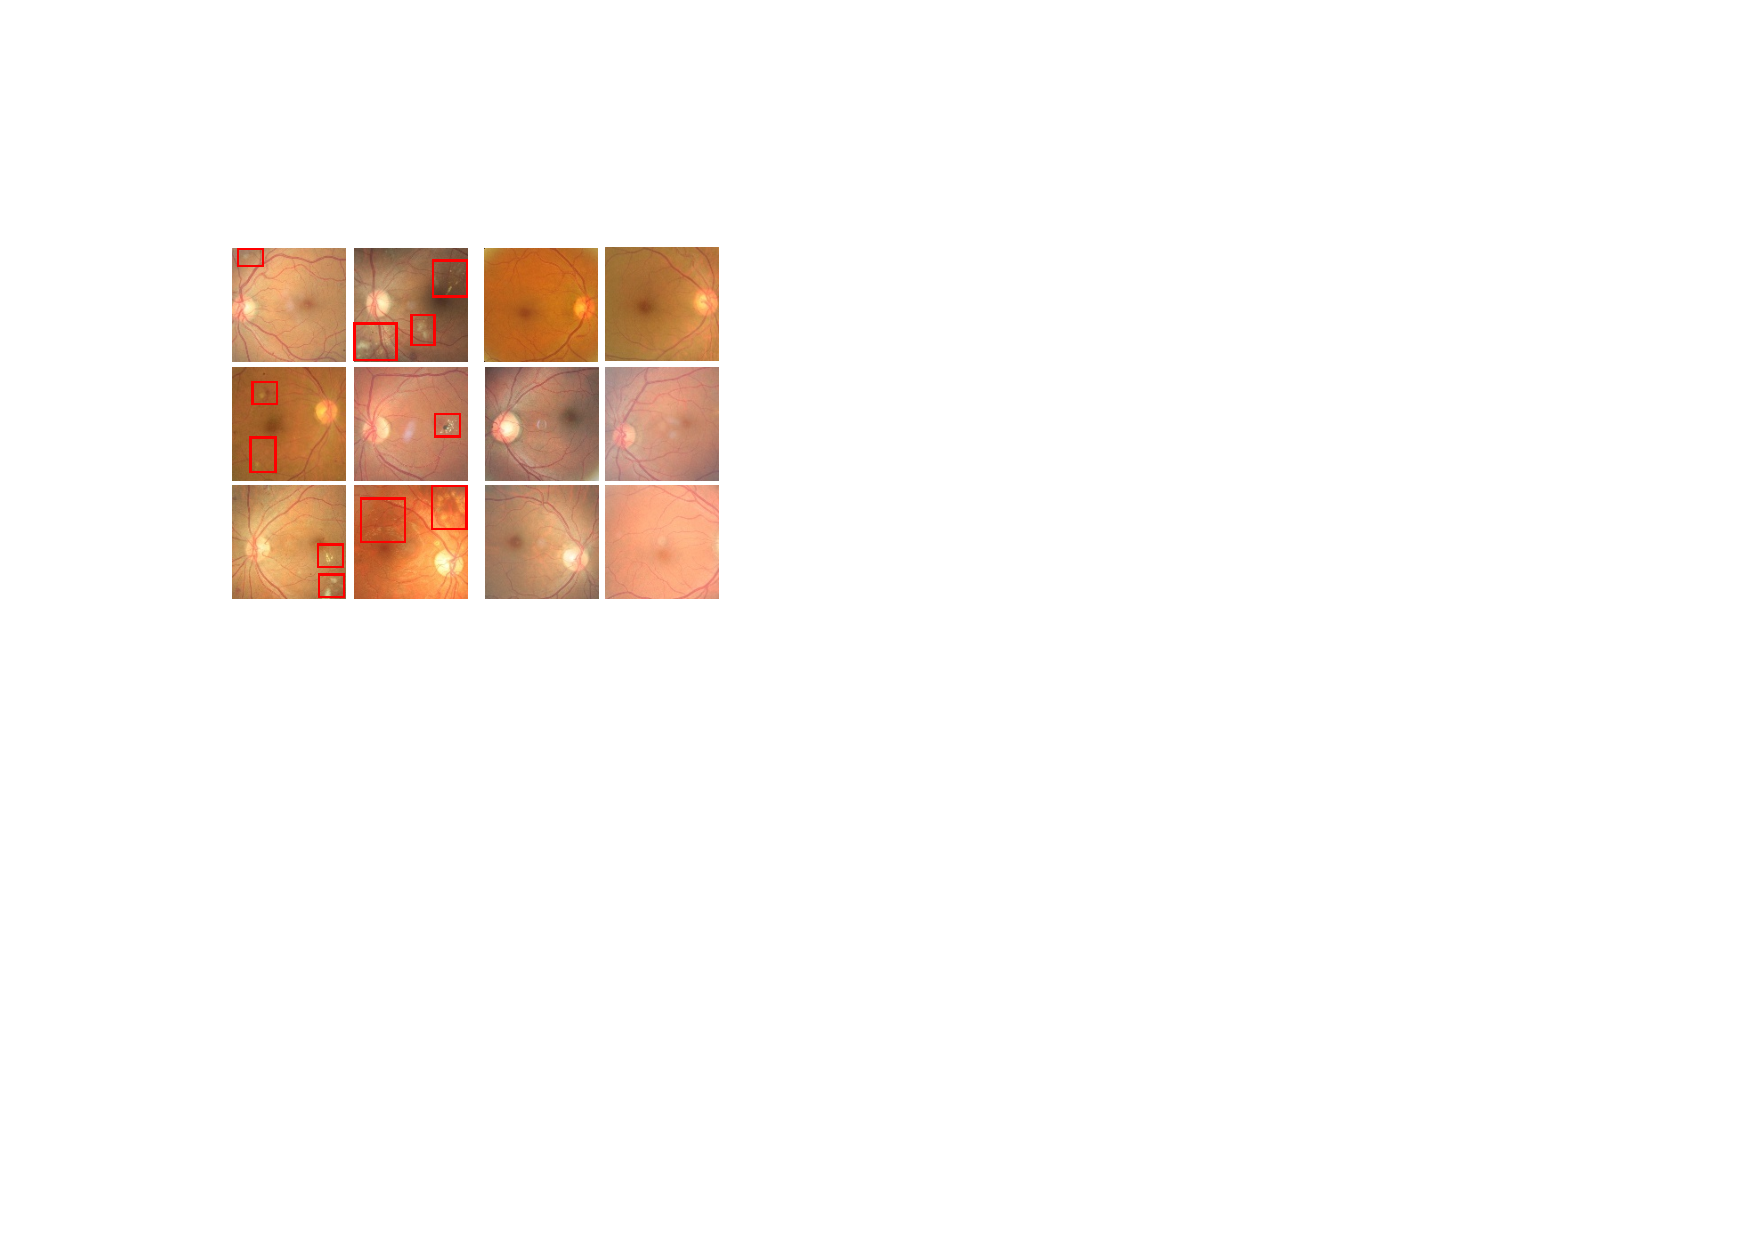
\includegraphics[width=1\textwidth]{figure/bin_dr_ds_example}
		\caption{二类视网膜糖尿病病变数据集部分图像示例。第1、2列是异常图像,第3、4列是正常图像。}
		\label{subfig:bin_dr_ds_example}
	\end{subfigure}
	\quad
	\begin{subfigure}{0.48\textwidth}
		\centering
		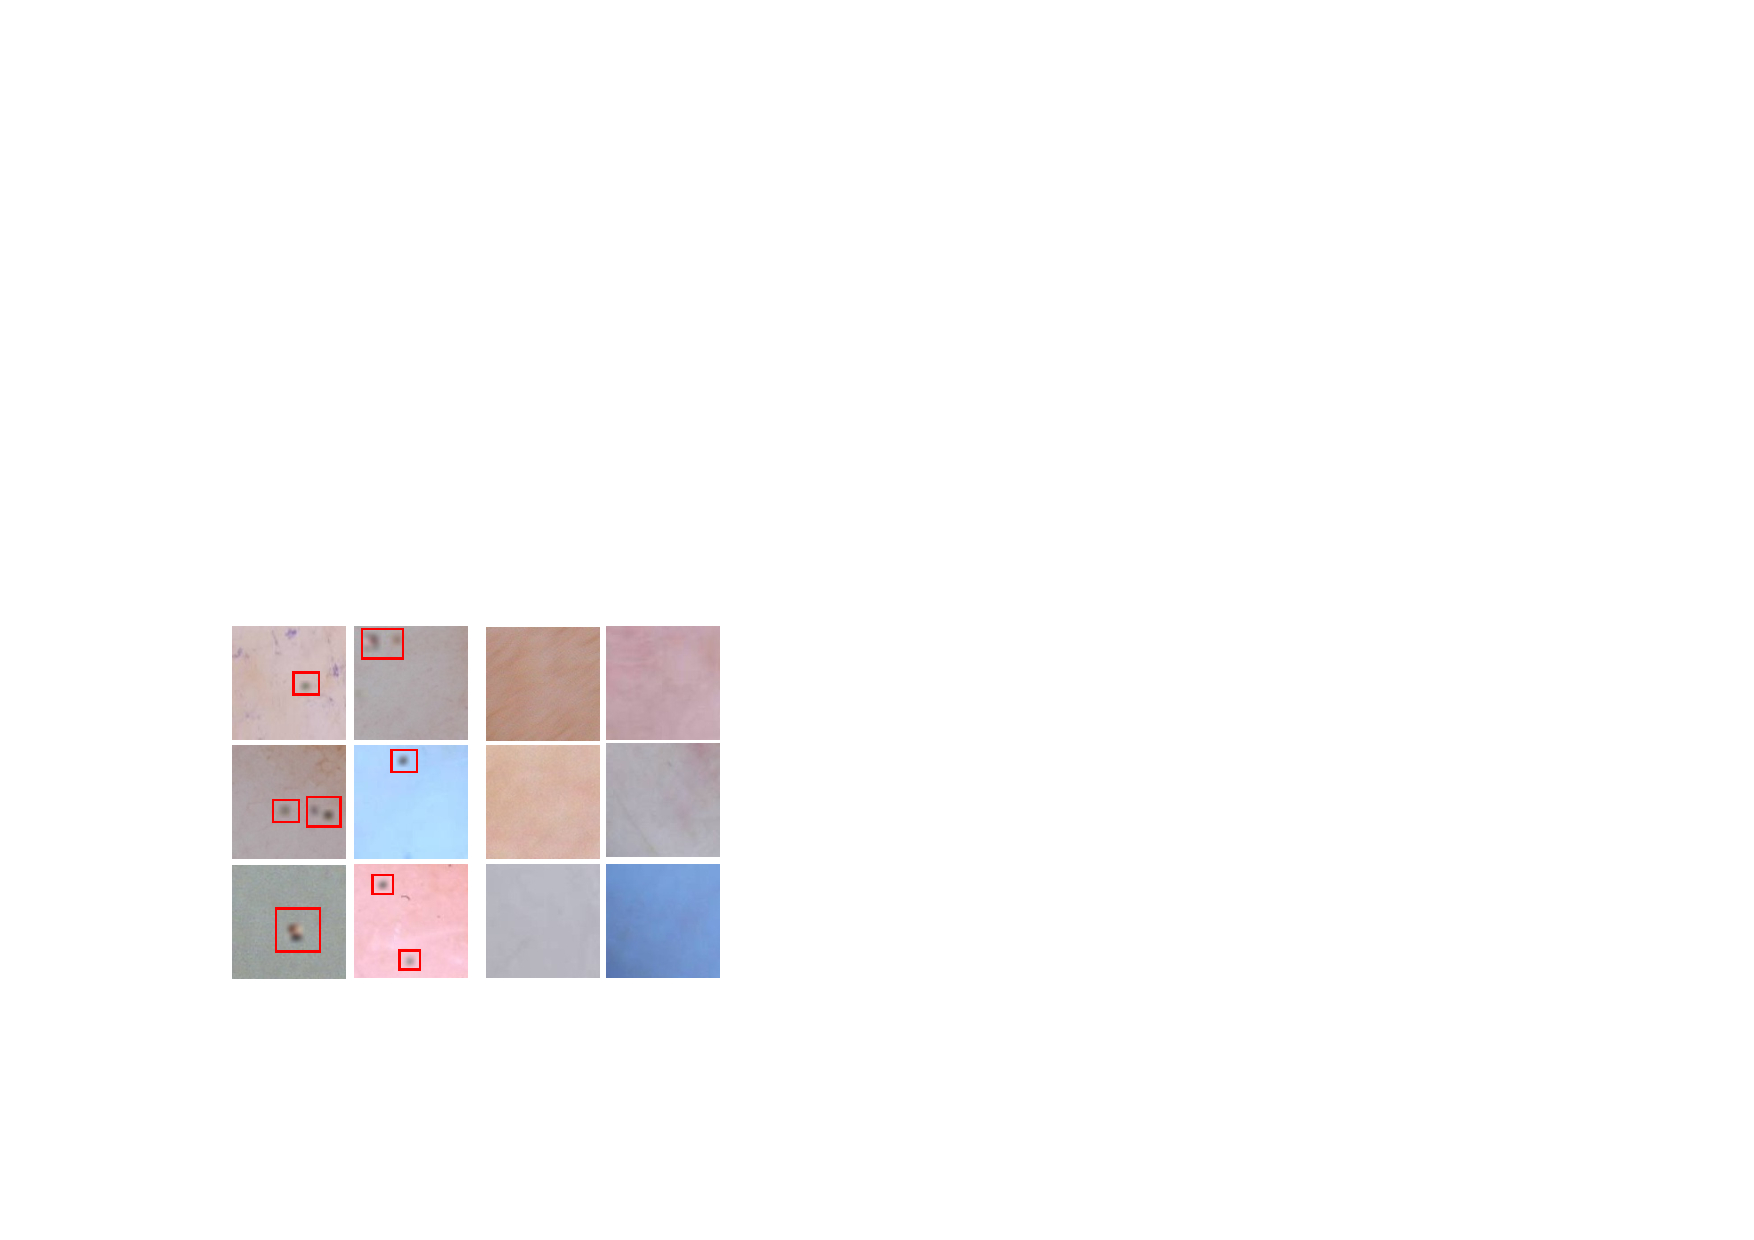
\includegraphics[width=1\textwidth]{figure/bin_simulate_skin_example}
		\caption{二类模拟皮肤病病变数据集部分图像示例。第1、2列是异常图像,第3、4列是正常图像。}
		\label{subfig:bin_simulate_skin_example}
	\end{subfigure}
	\caption{来自二类视网膜糖尿病病变数据集和二类模拟皮肤病病变数据集的部分图像示例。红色矩形框表示框内存在疾病标记物或者说框出区域是患病区域。在子图\ref{subfig:bin_dr_ds_example}中,每张图像中明显比周围要亮的圆形区域为视盘,为眼底图像的共有结构,而有些图像视盘在左边,有些视盘在右边,这是因为有些图像是左眼眼底图像,而有些是右眼眼底图像。}
	\label{mul_fig:bin_ds_example}
\end{figure}
\section{评价标准}\label{sec:exper_evaluation_metrics}

%在\ref{subsec:roc_curve}小节和\ref{subsec:pr_curve}小节中,本文分别介绍了ROC曲线及其AUC和P-R曲线及其AUC,并在此过程中定义了FPR、TPR等相关概念。本文还在\ref{subsec:pr_curve}小节中说明了ROC曲线对正负样本分布的变化表现比较稳定,而P-R曲线在此情况下则更为敏感,故P-R曲线更能反映出在正负样本比例悬殊较大情况下系统的真实性能。
在\ref{sec:evaluation_metrics}小节中,本文分别介绍了ROC曲线和P-R曲线及其各自AUC,并说明了在正负样本比例悬殊较大情况下,P-R曲线更能反映出系统的真实分类性能。从表\ref{tab:bin_ds_pixel_freqs}可以看出,无论是二类视网膜糖尿病病变数据集还是二类模拟皮肤病病变数据集,异常像素(正样本)和正常像素数量(负样本)之间的比例存在巨大悬殊甚至达到$88:1$(二类视网膜糖尿病病变数据集),故接下来的实验均采用P-R曲线及其AUC作为主要评价标准,但是ROC曲线也会在本文附录\ref{chapter:append1}中进行展示,实验评估从而更为全面,对相关内容感兴趣的读者可自行查看。

对于正常图像输入,我们期望编码器-解码器输出仍保持正常,反之,对于异常图像输入,我们期望编码器-解码器能将其转化为正常图像输出。为此,本文引入特异性(Specificity)和召回率(Recall)分别来衡量经过编码器-解码器之后的正常图像的保持率和经过编码器-解码器的异常图像的转化率。

\begin{table}[h]
	\centering
	\caption{二类视网膜糖尿病病变数据集和二类模拟皮肤病病变数据集图像像素数量统计表。}
	\label{tab:bin_ds_pixel_freqs}
	\begin{tabular}{c|c|c|c}
		\toprule[2pt]
		数据集名称 & 正常像素数量 & 异常像素数量 & 比例 \\
		\midrule[2pt]
		二类视网膜糖尿病病变数据集&  $643,837$ & $11,523$ & $\simeq 56: 1$ \\ \hline
		二类模拟皮肤病病变数据集 & $21,222,487$ & $240,553$ & $\simeq 88: 1$ \\
		\bottomrule[2pt]
	\end{tabular}
\end{table}


\section{实验设置}\label{sec:exper_setting}

本文所有实验相关代码实现均采用当前流行的深度学习框架PyTorch\footnote{https://pytorch.org/}。编码器-解码器模块选择一个经过修改的U-Net~\cite{iglovikov2018ternausnet}(详细结构修改请参见\ref{subsec:encoder_decoder_model}小节)。CNN分类模块采用Resnet-18,判别器模块使用一个$7$层卷积神经网络($4$个DownConv2d模块+$3$个Conv2dBlock模块,更直观地模型结构请对照图\ref{fig:discrimintor_architecture})。GAN采用WGAN-GP。为了让U-Net更好地重构图像,本文先将U-Net在数据集上进行预训练。

在预处理阶段,对于二类视网膜糖尿病病变数据集,我们先将图像中没有信息的四个黑角去掉;另外,由于眼底图像中的视网膜基本是呈圆形的,我们提取了视网膜的边界再根据视网膜边界取其最大内接矩形,从而彻底去掉眼底图像中的不包含任何信息的黑色部分,最后将图像尺寸大小重新调整到$128\times128$,最终得到二类视网膜糖尿病病变数据集。在图像数据送入模型训练之前,我们将输入减去$0.5$随后除以$0.5$,将输入变换到$[-1,1]$。在实验超参数设定方面,WGAN-GP中的梯度惩罚系数$\lambda$被设置为$10$(与WGAN-GP原文中一致)。模型训练使用Adam优化器~\cite{kingma2014adam},其中,对于CNN分类器,$\beta1$和$\beta2$分别设为$0.9$和$0.999$,对于生成器和判别器,$\beta1$和$\beta_2$分别设为$0.3$和$0.9$,默认学习率取$0.0002$,训练每次迭代取32张图像。对于所有的测试,$\lambda_1 = 0.4$和$\lambda_{2} = 10.0$。在生成P-R曲线之前,定位结果的热图被归一化为$[0,1]$。

%请注意,ROC曲线并不适合用来评价疾病标记物的定位性能,因为每个数据集的正、负像素的比例非常不平衡(参考表$\ref{tab:bin_ds_pixel_freqs}$)。因此,本文正文中只展示相关实验的P-R曲线。

请注意,我们的目标是通过图像级标签从已有图像中搜索和定位生物生物标记(像素级),而不是训练模型从新图像中寻找疾病标记物。因此,对于每个数据集,所有的图像都被用来训练我们的模型,然后对模型进行定性和定量的评估。因此,我们没有设置额外的验证集,将在相同的数据集上训练和评估我们的模型。基于同样的原因,在训练阶段,我们也没有采用随机翻转、随机裁剪等数据增广手段。

\section{在二类视网膜糖尿病病变数据集上的疾病标记物定位}\label{sec:bin_dr_ds_experiment}
本节将展示本文提出的模型在视网膜糖尿病病变数据集上的实验结果,本文提出的模型将与CAM和Grad-CAM共计两种用于卷积神经网络可视化方法作定性分析和定量分析。

CAM和Grad-CAM最为一种用于CNN可视化的方法,本身需要分两步完成。需要先训练得到一个分类器,再通过特征图的可视化来间接完成疾病标记物的定位。一方面为了尽量减少与实验内容无关的因素干扰,另一方面由于CAM只能完成对最后一层是全局均值池化层的卷积神经网络的可视化(相关解释可参见\ref{subsec:gradient_based_methods}小节),综合以上因素,本文将ResNet-18作为CAM和Grad-CAM可视化的目标CNN分类器。另外,为了排除由于CNN性能的缺陷导致可视化结果表现较差,本文同样使用数据集中的所有图像来训练ResNet-18分类器,即没有为ResNet-18单独设置测试集,本文后续所有关于CAM和Grad-CAM的相关实验结果均在此条件设置下完成。在使用视网膜糖尿病病变数据集训练ResNet-18时,分类器最终的分类准确率达到了100\%。由于Grad-CAM可对任意层输出的特征图完成可视化,从而实现疾病标记物的定位。因此,如图\ref{fig:retinal_image_res}所示,本文展示出了使用Grad-CAM对中间层特征输出(第$4$列)和最后一层特征输出(第$5$列)的疾病标记物定位结果(可与CAM作比较)。
\begin{figure}[h]
	\centering
	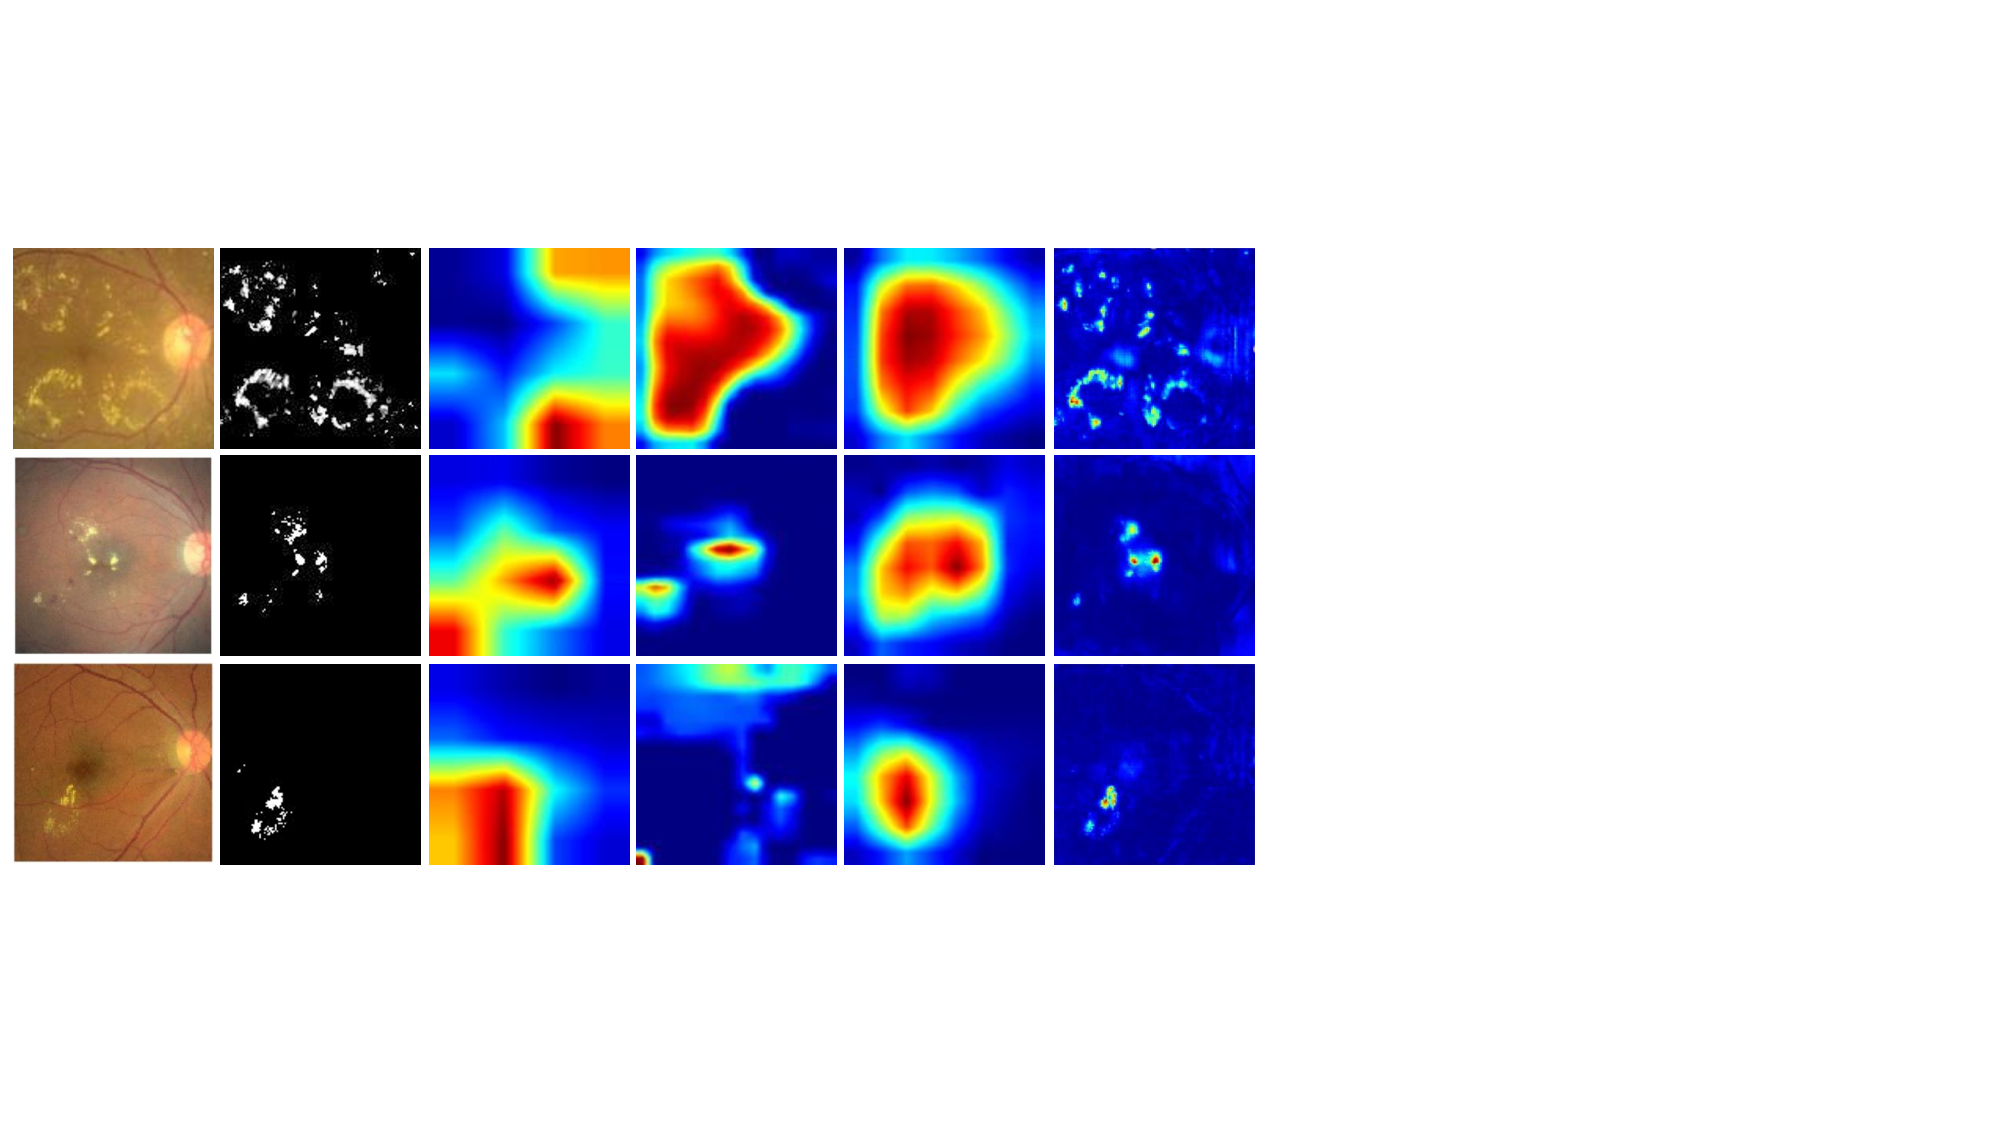
\includegraphics[width=1.0\textwidth]{figure/retinal_image_res.pdf}
	\caption{在视网膜糖尿病病变数据集上疾病标记物定位结果。图中第$1$列表示原始异常图像,第$2$列表示其像素级标注,第$3$列表示CAM的定位结果,第$4$列表示Grad-CAM使用分类器中间层的特征图可视化的定位结果,第$5$列表示Grad-CAM使用分类器最后一层特征图可视化的定位结果,第$6$列是本文提出模型的定位结果。第$3-6$列表示输入图像的定位结果的热图,图中某一区域颜色越红,表示该区域为疾病标记物的可能性越高。蓝色表示的意义与红色相反,表示其所在区域是疾病标记物的可能性越低。以上颜色代表的意义同样适用于下文所有热图。}
	\label{fig:retinal_image_res}
\end{figure}

\noindent 如图\ref{fig:retinal_image_res}所示,从图中第$3$列定位结果可以看出,虽然CAM发现的疾病标记物或者说异常区域最多,但是CAM也将周边区域作为疾病标记物的一部分。这主要是由于将最后一个卷积层($4\times 4$)的输出向上采样到图像大小($128\times 128$)。另外,CAM也未能检测到第一幅图像(第$3$列,第$1$行)中的大部分异常区域。Grad-CAM作为CAM的扩展,它允许我们从多个层生成可视化的解释,例如中间卷积层(第$4$列,可记为Grad-CAM-1)和最后卷积层(第$5$列,可记为Grad-CAM-2)。虽然Grad-CAM-1在第$4$列(第三幅图像)获得了较为准确的疾病标记物定位结果,但通过也将正常区域(图像中中间上方区域和左下角区域)误认作包含疾病标记物的异常区域。更多的是其结果要么不够精确(第$1$行),要么不够精确(第$2$行和第$3$行)。与CAM相比,Grad-CAM-1实现了更为精确的定位结果,证明了其优于CAM的性能。另外,同样是由于对可视化特征图悬殊的上采样倍数($4\times 4 \rightarrow 128\times 128$),可以发现,Grad-CAM-2(第$5$列)标记的区域和CAM(第$3$列)没有太大区别。相比之下,本文提出的方法对形状不规则、分布分散的疾病标记物进行了更精确的局部化(第$6$列),从定性分析的角度证明了其优于CAM和Grad-CAM的性能。

\begin{figure}[h]
	\centering
	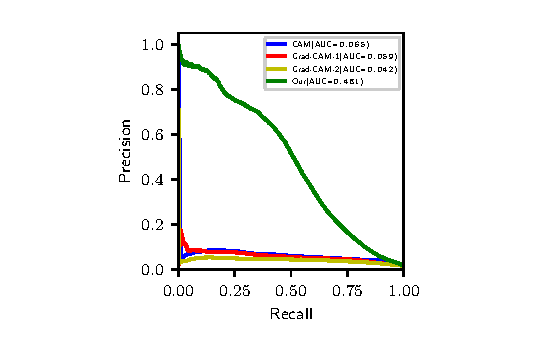
\includegraphics[width=1.0\textwidth]{figure/pr_curve_retinal_image/pr_curve.eps}
	\caption{CAM、Grad-CAM-1、本文提出的模型和Grad-CAM-2在40张视网膜糖尿病病变图像上画出的P-R曲线及其各自曲线下的面积(AUC,见右上角图例)。} 
	\label{fig:retinal_image_pr_curve}
\end{figure}

另外,本文充分利用二类视网膜糖尿病病变数据集中的$40$张像素级标注,通过对每种方法的定量评价,本文提出的模型、CAM、Grad-CAM-1和Grad-CAM-2的P-R曲线如图\ref{fig:retinal_image_pr_curve}所示。可以发现,绿色P-R曲线在其他三条曲线的上方,且与下侧横轴和左侧纵轴围成的封闭区域面积显然最大。以上四种方法各自对应的P-R曲线下的面积(AUC)分别为$0.481$,$0.065$,$0.061$和$0.042$,从而进一步从定量分析的角度证明了本文提出的模型在二类视网膜糖尿病病变数据集上的性能优越性。

\section{在二类模拟皮肤病病变数据集上的疾病标记物定位}\label{sec:bin_simulated_ds_experiment}
本节将展示本文提出的模型在模拟皮肤病病变数据集上的实验结果分析,本文提出的模型的比较对象同样是与CAM和Grad-CAM共计两种CNN可视化方法进行比较,分定量分析和定性分析两个角度展开。

与\ref{sec:bin_dr_ds_experiment}小节一样,在本实验中,依然将ResNet-18作为CAM和Grad-CAM可视化的目标CNN分类器,同样没有单独设置测试集,分类器最终CNN分类准确率均达到了$99.7\%$以上。类似的,由于Grad-CAM可对卷积神经网络的任意层输出特征进行可视化,故在此实验中,同样选择了中间层输出特征(见图\ref{fig:simulated_skin}第$4$列)和最后一层输出特征(见图\ref{fig:simulated_skin}第$4$列)进行可视化,从而定位疾病标记物。
\begin{figure}[h]
	\centering
	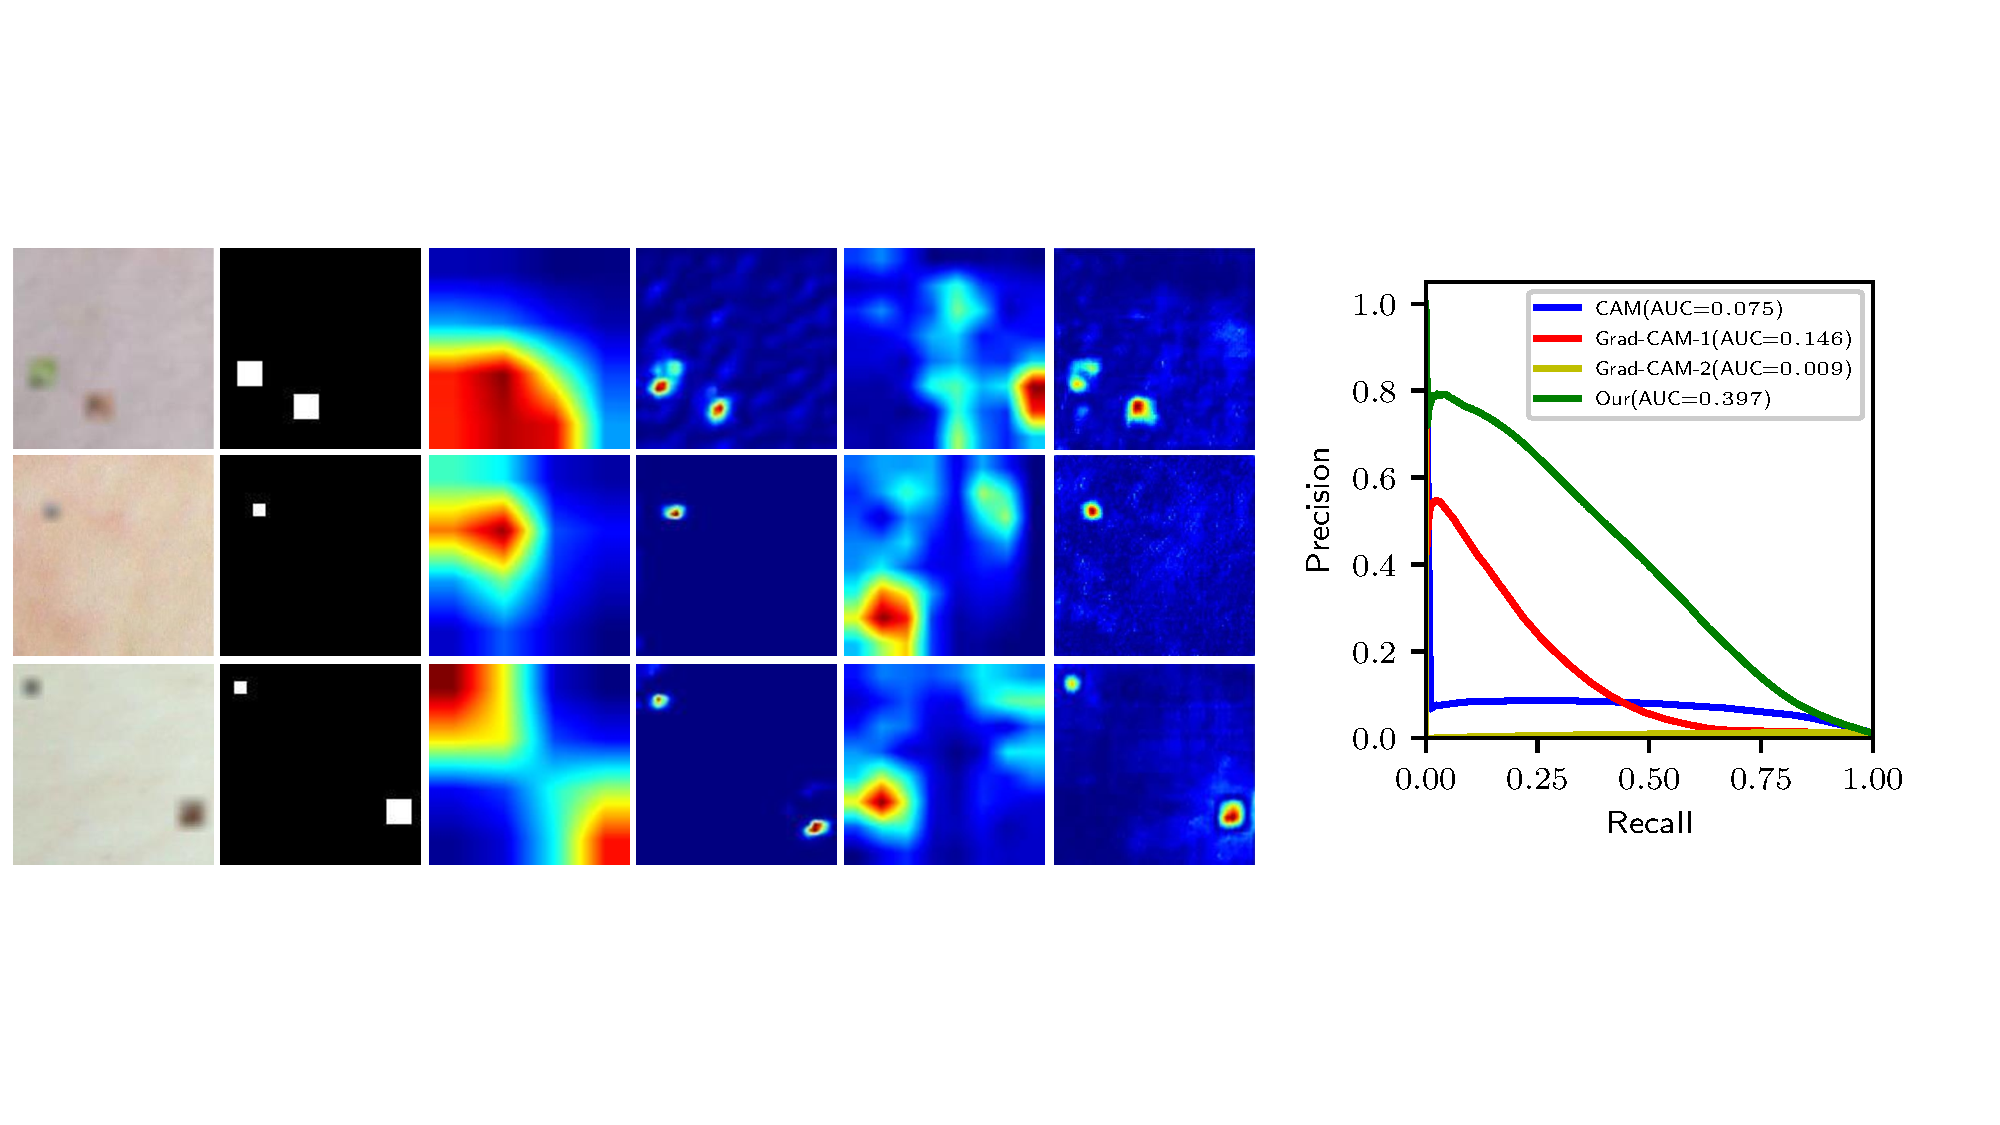
\includegraphics[width=1.0\textwidth]{figure/pr_curve_skin_image.pdf}
	\caption{在二类模拟皮肤病病变数据集上的疾病标记物定位结果。图中第$1$列表示原始异常图像,第$2$列表示其像素级标注,第$3$列表示CAM的定位结果,第$4$列表示Grad-CAM使用分类器中间层的特征图可视化的定位结果(Grad-CAM-1),第$5$列表示Grad-CAM使用分类器最后一层特征图可视化的定位结果(Grad-CAM-2),第$6$列是本文提出模型的定位结果。} 
	\label{fig:simulated_skin}
\end{figure}

\noindent 从图\ref{fig:simulated_skin}可以看出,人工模拟生物标志物的皮肤图像进一步证实了本文提出的模型的优越性能。从图\ref{fig:simulated_skin}第$6$列可以看出,本文提出的方法几乎可以完美、精确地定位人工疾病标记物,而CAM(第$3$列)和Grad-CAM(第$4$列和第$5$列)的性能再次表现出劣势。从总体上来说,第$4$列中疾病标记物定位结果明显要比第$3$列更精确、更完美,也就能说明Grad-CAM在定位疾病标记物上优于CAM。同样是由于特征图的过度上采样,CAM(第$3$列)和Grad-CAM-2(第$5$列)呈现类似的定位结果:虽然能检测到疾病标记物的位置,但同时也包含了疾病标记物周围的大量正常像素。之所以Grad-CAM-1(第$4$列)基本能精确定位到疾病标记物的位置而极少包含疾病标记物的周围像素,主要是因为Grad-CAM-1是通过对ResNet-18中第一个卷积层的特征输出的可视化结果来完成疾病标记物的定位,其中上采样倍数较小($64\times 64\rightarrow 128\times 128$),这也能从侧面说明在该数据集上定位疾病标记物要比在二类视网膜糖尿病病变数据集上容易得多(浅层特征便具备高级语义)。而CAM和Grad-CAM-2却都选择了最后一层卷积层的输出特征,其中上采样倍数要大得多($4\times4\rightarrow 128\times 128$)。

与CAM和Grad-CAM相比,图\ref{fig:simulated_skin}从定性分析的角度证明了本文提出的方法在二类模拟皮肤病病变数据集上的性能优越性,图\ref{fig:simulated_skin_pr_curve}再次从定性分析的角度证明了这一结论。CAM、Grad-CAM-1、Grad-CAM-2和本文提出的模型根据二类模拟皮肤病病变数据集上所有标注所得出的P-R曲线如图\ref{fig:simulated_skin_pr_curve}所示。不难看出,图中绿色曲线明显在其他三条曲线的上方,与下侧横轴和左侧纵轴围成的封闭区域的面积上,绿色曲线也明显大于其他三条曲线。以上四种方法各自对应的P-R曲线的AUC分别是$0.075$、$0.146$、$0.009$和$0.397$。
\begin{figure}[h]
	\centering
	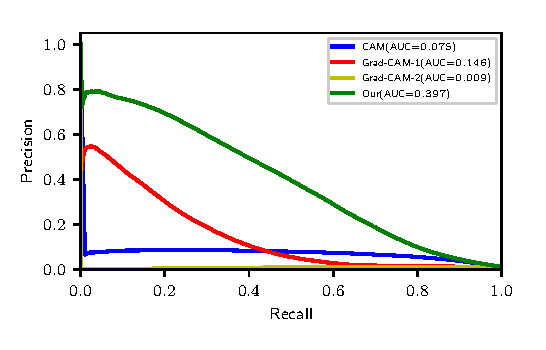
\includegraphics[width=1.0\textwidth]{figure/pr_curve_skin_image/pr_curve.eps}
	\caption{CAM、Grad-CAM-1、本文提出的模型和Grad-CAM-2在$1,310$张模拟皮肤病病变图像上画出的P-R曲线及其各自曲线下的面积(AUC,见右上角图例)。}
	\label{fig:simulated_skin_pr_curve}
\end{figure}

\section{CNN分类器和判别器角色探究}\label{sec:g_c_g_d_g_d_c_comparsion}
在\ref{sec:bin_dr_ds_experiment}小节和\ref{sec:bin_simulated_ds_experiment}小节中,本文通过定性分析和定量分析两个角度在二类视网膜糖尿病病变数据集和二类模拟皮肤病病变数据集上证明了本文提出的模型在疾病标记物定位上的优越性能。为了进一步探究本文提出的模型中各个子模块在视网膜糖尿病病变图中扮演的角色以及添加的必要性(相关内容参见\ref{subsec:model_architecture}小节),本节内容将完成消融实验,分别去掉本文提出的模型中的CNN分类器和判别器,以探究CNN分类器模块和判别器模块的在整个模型中所起的作用。为了方便后续内容叙述,对于本文提出的模型,本文将其记为G-D-C模型,将移除判别器模块之后的模型记作编码器-解码器-CNN分类器(G-C)模型,将移除CNN分类器模块之后的模型记作编码器-解码器-判别器G-D模型。G-D-C模型、G-C模型和G-D模型的在二类视网膜糖尿病病变数据集上的部分实验结果如图\ref{fig:u_d_c_comparation}所示。
\begin{figure}[h]
	\centering
	\includegraphics[width=1.0\textwidth]{figure/u_d_c_comparation.pdf}
	\caption{G-D-C模型、G-C模型和G-D模型的在二类视网膜糖尿病病变数据集上的部分实验结果展示。第$1$列是原始输入图像,其中第一行是正常图像输入,第$2-4$行是异常图像输入。第$2$列是G-C模型的输出定位结果,第$3$列是第$2$列与第$1$列的差,第$4$列是G-D模型的输出定位结果,第$5$列是第$4$列与第$1$列的差,第$6$列是G-D-C模型给出的定位结果,第$7$列是第$6$列与第$1$列的差。第$4$列图像中的红色框表示其圈出部分的血管与原始输入图像相比发生了改变。} 
	\label{fig:u_d_c_comparation}
\end{figure}

从图\ref{fig:u_d_c_comparation}可以看出,当输入图像是正常图像时(图中第$1$行),G-D-C模型、G-C模型和G-D模型均能几乎不改变图像中的像素强度,只有在借助图中第$5$列和第$7$列的热图才能看出这张正常图像的左上角有些许改变。这说明对于正常图像,以上三种模型均能处理得比较好,以上三种模型的性能差异主要表现在处理异常图像(图中第$2-4$行)上。不难看出,在没有判别器的情况下(G-C模型),CNN分类器只能帮助定位了部分疾病标记物(图中第$3$列热图),而将大部分疾病标记物留在了编码器-解码器的输出(图中第$2$列)中。另一方面,在没有CNN分类器的情况下(G-D模型),判别器能定位到大部分(如果不是全部的话)的疾病标记物区域(图中第$5$列)。然而,我们注意到,一些正常区域的像素强度同样也发生了改变(我们在第$4$列中用红色矩形框圈出),导致了一些正常的像素被错误得标记为疾病标记物,包括一些包含血管的区域,这种发生改动的血管区域在第$5$列的热图中现实得更加突出。相比之下,编码器-解码器与CNN分类器以及判别器的组合(G-D-C模型)不仅可以精确定位大部分的疾病标记物(图中第$7$列),在编码器-解码器的输出端(第$6$列)还能标记较少的假阳性疾病标记物(图中第$7$列热图和第$5$列热图相比较)和更多的真实疾病标记物(第$7$列热图和第$3$列热图相比较)。如\ref{sec:model_architecture_intro}小节描述,这些结果表明分类器和鉴别器网络共同帮助定位生物标志物。就各自角色而言,CNN分类器可在图像中定位疾病标记物并在一定程度上帮助帮助编码器-解码器去除疾病标记物(图中第$3$列),而判别器帮助编码器-解码器进一步去除CNN分类器未能定位或者未能去除的、难以去除的疾病标记物。两者相辅相成(第$3$列与第$7$列比较),共同帮助编码器-解码器尽量去除图像中的所有疾病标记物(图中第$7$列)。

\begin{figure}[h]
	\centering
	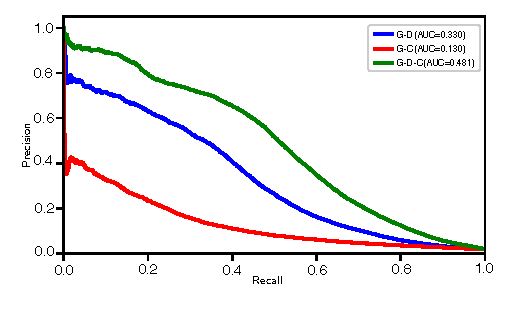
\includegraphics[width=1.0\textwidth]{figure/pr_cureve_u_d_u_c_u_d_c_components.pdf}
	\caption{G-D模型、G-C模型和G-D-C模型根据二类视网膜糖尿病病变数据集中标注的部分图像绘制的P-R曲线。三条曲线各自对应的AUC见右上角图例。} 
	\label{fig:u_d_c_comparation_pr_curve}
\end{figure}

为了对G-D模型、G-C模型和G-D-C模型进行更为精确的定量评价,本文再次使用二类视网膜糖尿病病变数据集中的$40$张像素级标注图像,进一步证实了以上结论。三者的P-C曲线如图\ref{fig:u_d_c_comparation_pr_curve}所示。可以发现,图中绿色的P-R曲线(G-D-C模型)在紫色(G-D模型)以及红色(G-C模型)P-R曲线上方,在曲线与左侧纵轴和下侧横轴围城的面积方面,绿色曲线显然围住了紫色以及红色P-R曲线,G-D-C模型(绿色曲线)、G-D模型(紫色曲线)和G-C模型(红色曲线)各自P-R曲线对应的AUC分别为$0.330$、$0.130$和$0.481$。这些现象再次表明G-D-C模型在视网膜糖尿病病变图像上的性能表现要优于G-D模型和G-C模型,同时也说明了CNN分类器和判别器的不可或缺行,符合\ref{subsec:model_architecture}小节中对二者的角色设计和期望。

另外,基于\ref{sec:idea_thinking}小节中的朴素思路,我们只使用正常图像训练编码器-解码器,希望编码器-解码器具有重建正常信号的能力,从而间接实现疾病标记物的定位,本文将此素朴思路记为基准方法。然而,在二类视网膜糖尿病病变数据集上得到的AUC为$0.083$,远远低于G-C模型、G-D模型和G-D-C模型在此数据集上得到的结果(三者得到的AUC分别为为$0.130$、$0.330$和$0.481$),三者者均远远高于基准方法(更为直观的实验数据参见表\ref{tab:baseline_compared_diabetic_ds}),也能说明引入CNN分类器和判别器的必要性,从而再次佐证上述结论。
\begin{table}[h]
	\centering
	\caption{基准模型、G-C模型、G-D模型和G-D-C模型在二类视网膜糖尿病病变数据集上的实验结果表。表格展示的是通过P-R曲线计算的AUC分数。}		
	\label{tab:baseline_compared_diabetic_ds}
	\begin{tabular}{c|c|c|c|c}
		\toprule[2pt]
		模型名称 & 基准模型 & G-C模型 &G-D模型&G-D-C模型 \\
		\midrule[2pt]
		AUC	& $0.083$&	$0.130$ & $0.330$ & $\textbf{0.481}$	 \\
		\bottomrule[2pt]
	\end{tabular}
\end{table}

\section{对于经过编码器-解码器的视网膜糖尿病病变图像的定量分析}\label{sec:indirect_quantitative_evaluation}
在\ref{sec:bin_dr_ds_experiment}小节和\ref{sec:bin_simulated_ds_experiment}小节中,本文在二类模拟皮肤病病变数据集和二类视网膜病变数据集上利用已有的数据像素级标注进行了定量分析,这方式可看做是一种直接验证的方式。在本节中,本文将从间接角度来再次验证本文提出的模型在处理疾病标记物定位问题的有效性。直观的想法是,在理想情况下,如果一种方法可以准确地定位和去除图像中的生物标记,则去除检测到的生物标记后的图像将不再包含疾病标记物,那么去除检测到的生物标记后的图像将很难与原来的正常图像区分开来。基于以上想法,本文将二类视网膜糖尿病病变数据集按照$80$\%和$20$\%的比例分为训练集和验证集,为下文叙述方便,下文简称该数据集为“原始数据集”,并用训练集数据训练一个ResNet-18二类分类器。随后,对于训练集和验证集,每个图像都被输入到训练之后的编码器-解码器中,所有编码器-解码器的输出图像被收集起来,从而得到一个新的数据集,为了后文叙述方便,本文将该数据集记为“‘正常’数据集”。最后,本文使用原始数据集训练得到的ResNet-18二类分类器对“正常”数据集分类。在此,为了分别衡量编码器-解码器将异常图像输入的转化能力和编码器-解码器对正常图像输入的保持能力,本文使用Recall和Specificity作为分类器的评价标准。相关实验结果如表\ref{tab:quantitative_retinal}所示。

\begin{table}[h!]
	\begin{center}
		\caption{原始二类视网膜糖尿病病变数据集和“正常”数据集在ResNet-18分类器上的分类结果。前两列表示在原始数据集上的实验结果,后两列表示“正常”数据集上的实验结果。} 
		\label{tab:quantitative_retinal}
		\begin{tabular}{c|cc|cc}
			\toprule[2pt]
			& \multicolumn{2}{c|}{原始数据集} & \multicolumn{2}{c}{“正常”数据集} \\
			&  训练集 & 验证集 & 训练集 & 验证集\\
			\midrule[2pt]
			Recall & $0.958$ & $0.936$ & $0.269$ & $0.292$\\ \hline
			Specificity & $0.984$ & $0.964$ & $0.980$ & $0.964$\\
			\bottomrule[2pt]
		\end{tabular} 
	\end{center}
\end{table}

从表\ref{tab:quantitative_retinal}不难看出,对于原始数据集(见表中前两列),ResNet-18分类器不仅在训练集上取得了较高的特异性(Specificity=$0.984$)和召回率(Recall=$0.958$),在测试集上也表现了优异性能(Recall和Specificity分别为$0.936$和$0.964$),说明ResNet-18分类器已经学会了寻找用于分类预测的疾病标记物的特征。另外,表\ref{tab:quantitative_retinal}中后两列显示,大多数“正常”数据集中的异常图像在训练集和验证集上都被错误地归类为正常,导致更低的召回率(训练集和验证集上的Recall分别为$0.269$和$0.292$),说明本文提出的模型能够很好地定位并去除原始异常图像中的疾病标记物,使得ResNet-18二分类器无法将去除疾病标记物的图像与原始正常图像区分开来。另一方面,ResNet-18分类器在正常图像上具有较高的特异性值(训练集和验证集上分别为$0.980$和$0.964$),说明经过编码器-解码器后的正常图像仍然被正确分类为正常图像,这证实了编码器-解码器不会改变正常输入,也从实验角度证明了在\ref{sec:idea_thinking}小节中对编码器-解码器的设想。总之,在原始数据集和“正常”数据集上,无论对于其中的训练集还是验证集,召回率的大幅下降和特异性的小幅下降表明,本文提出的模型可以很好地从图像中去除潜在的疾病标记物,同时保持正常区域不变。从而再次从CNN分类器的角度证明了本文提出的方法的优异性能。
\begin{figure}[h]
	\centering
	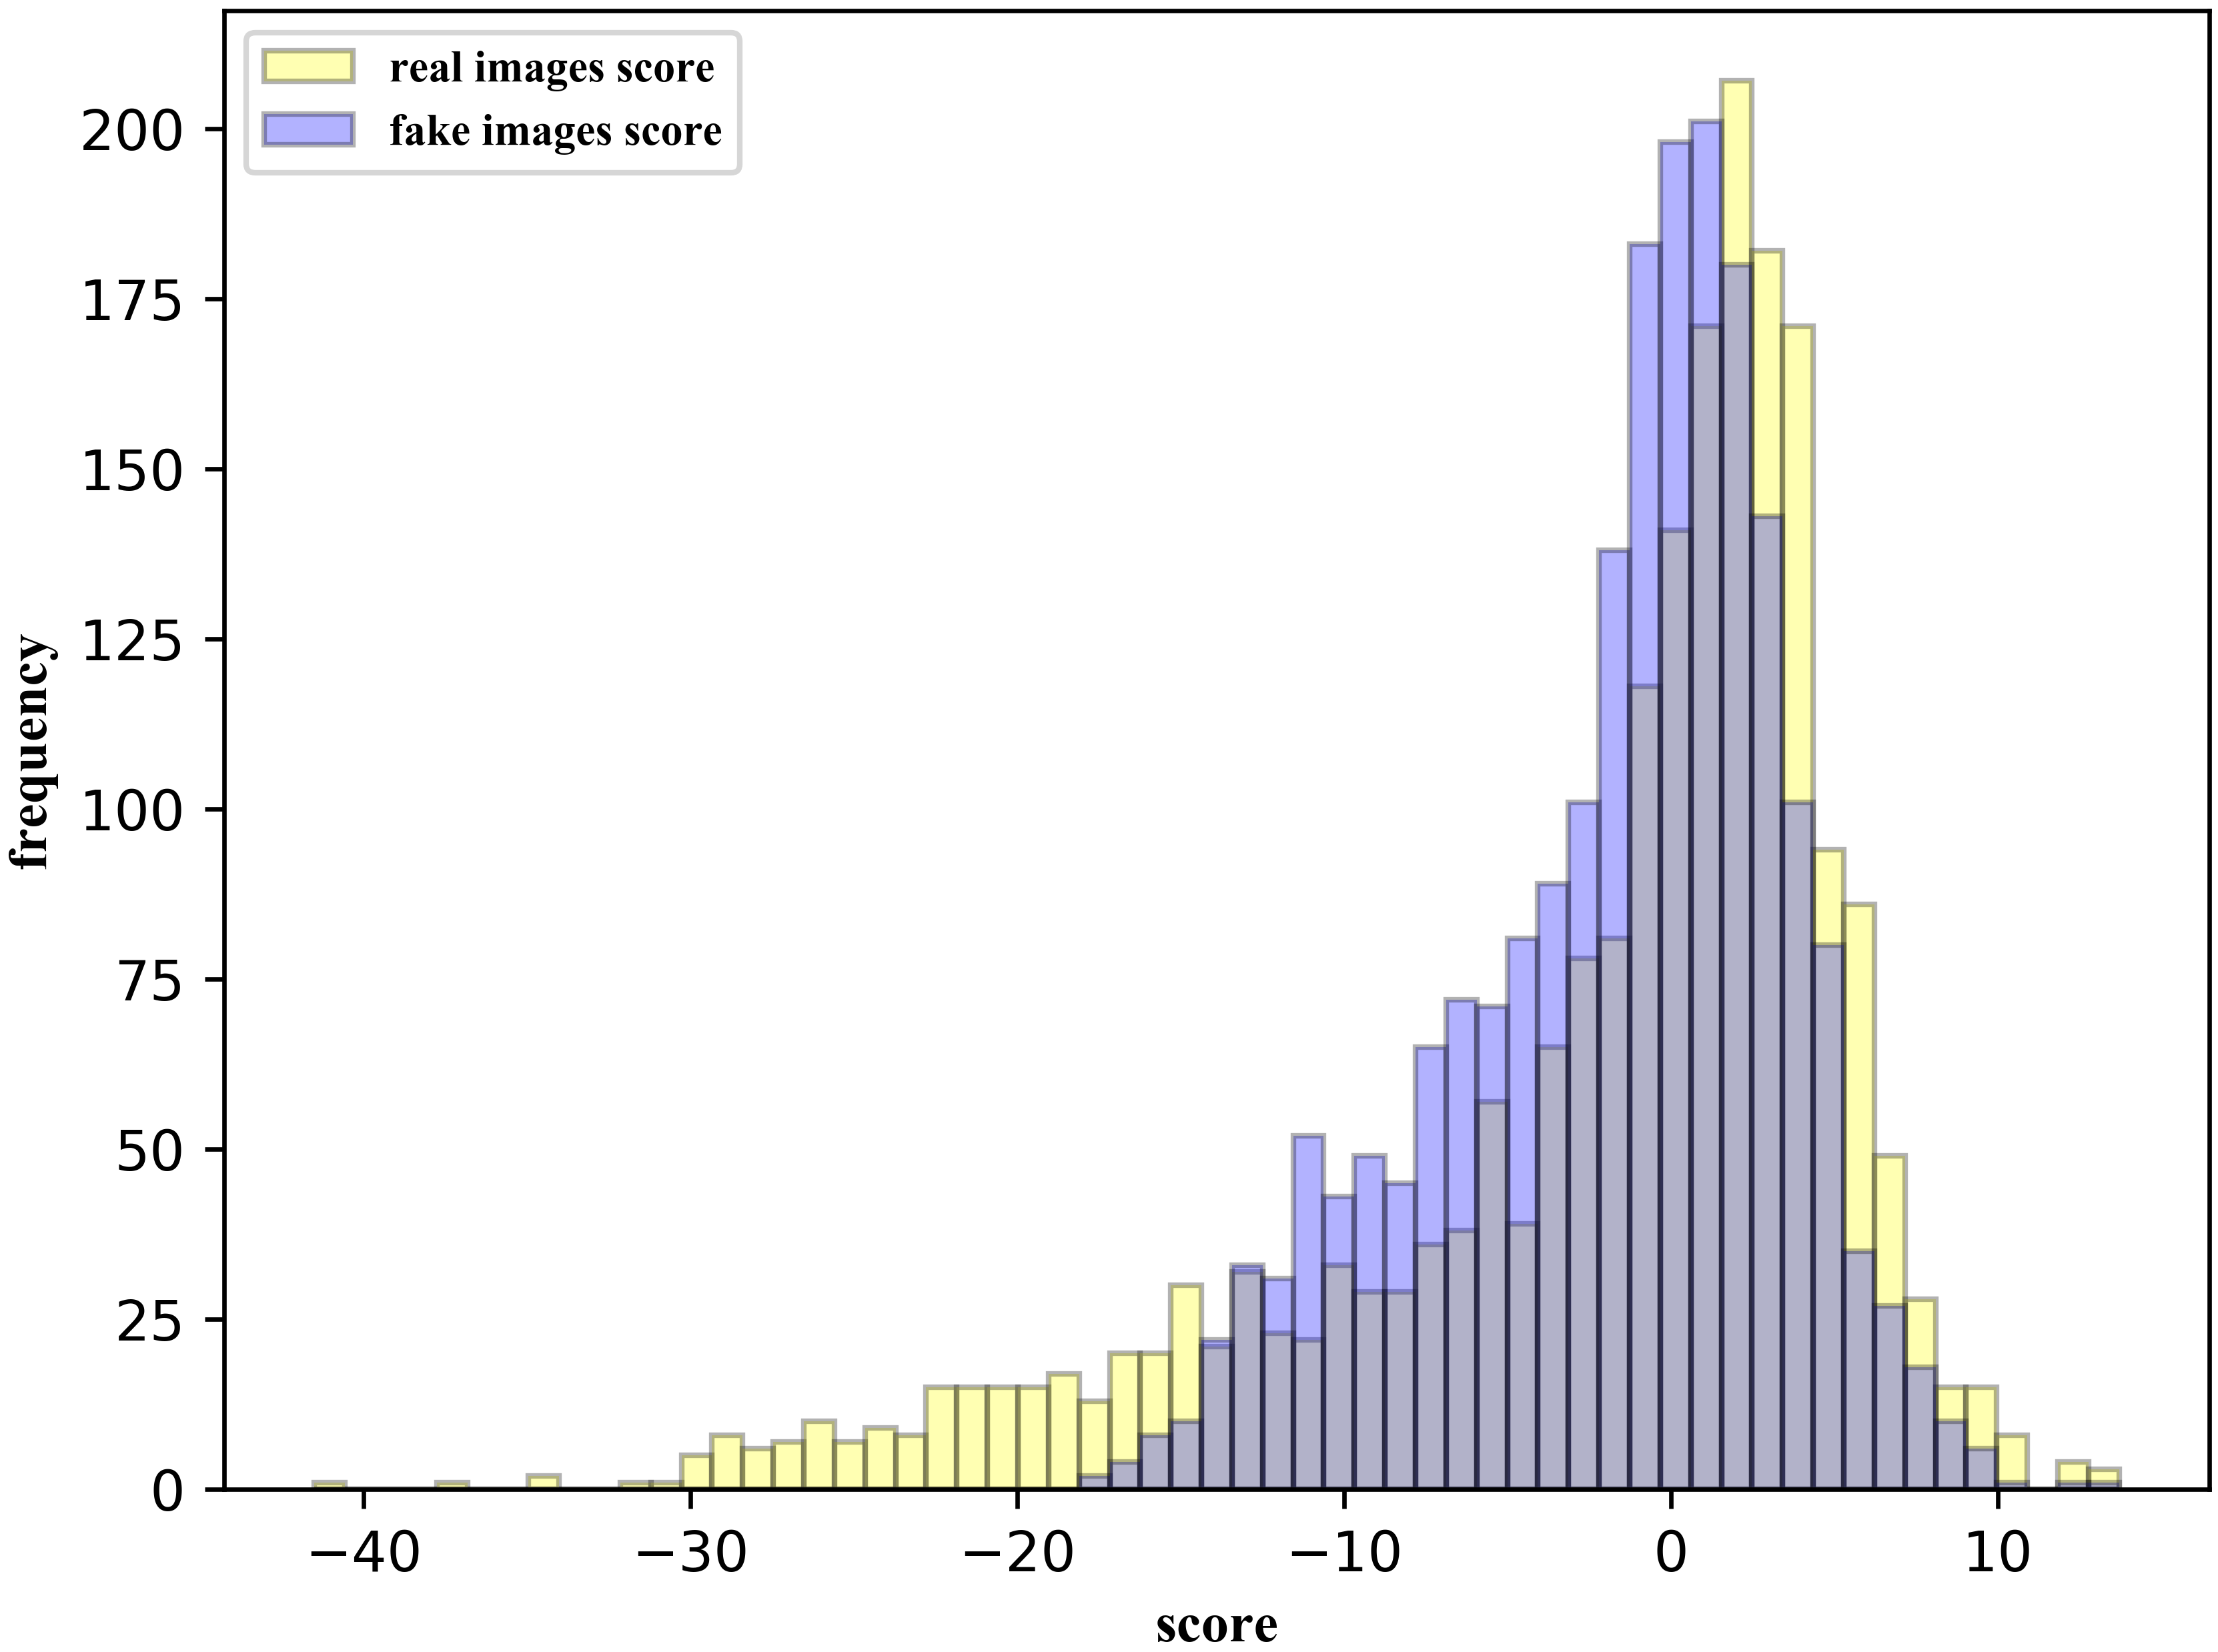
\includegraphics[width=1.0\textwidth]{figure/score_distribution.png}
	\caption{将原始数据集中的正常图像和“正常”数据集中的“正常”图像分别送入到判别器之后,根据输出分数绘制的频率分布直方图。黄色柱子表示判别器真图像输入端的输出分数,紫色柱子表示判别器假图像输入端的输出分数,灰色柱子表示以上两者的重叠部分。}
	\label{fig:hist_freq}
\end{figure}

另外,训练结束后,我们还将“正常”数据集中的正常图像和异常图像均送入判别器,判别器输出分数的频率分布直方图如图\ref{fig:hist_freq}所示。不难从直方图中看出,送入判别器的两端分数的频率分布直方图有较大重叠部分,如果暂时不考虑原始图像中的离群点(直方图中靠近下侧横轴最左端的分数),则两者分解输出分数会更加接近。我们还可以根据以上直方图可计算得到,判别器对于“正常”数据集中的正常图像和异常图像输出的平均输出分数分别为$-2.1$和$-1.7$,而在初始参数下,两者的平均分数分别为$-2.2$和$-1.0$,这说明训练结束后,判别器输出端的输入图像相似度得到极大提升(判别器两端输出平均分数的差值大大缩小:$1.2\rightarrow 0.4$)。总之,以上现象可说明,对于正常图像输入,编码器-解码器基本不改变其像素强度;而对于异常图像输入,经过编码器-解码器的输出与不断向正常图像输出靠近,也从判别器的角度间接说明编码器-解码能够比较好地去除原始数据集中的疾病标记物。


\section{对判别器模型结构的探究}\label{sec:dis_arch}
% 原始 D_FPN
% 对比跨层 D_NSC no skiping connection
% 去掉第一个下采样(高分辨率特征 用中间层 不用高分辨率特征融合) D_NLL no feature map from low layer
% 去掉最后一个下采样(不用中间层特征 只用高分辨率)D_NML no feature map from middle layer
在本节内容中,在保持其他设置不变的情况下,本文将设置一系列有关判别器结构的消融实验来探究不同判别结构对于最终定位结果的影响。判别器的网络结构可参见图\ref{fig:discrimintor_architecture},为了后文叙述方便,将原始判别器记作$\mathrm{D}_\mathrm{FPN}(i,j)$。为了探究跨层结构的影响,本文将去掉所有跨层结构的判别器记作$\mathrm{D}_\mathrm{NSC}(i,j)$。在原始判别器中,最后一个全连接层是由第一个下采样单元输出特征、最后一个下采样单元输出特征和最后一个网络单元输出特征融合得到,为了探究来自不同层次和不同分辨率特征融合的影响,本文将去掉第一个下采样单元特征输出而进行特征融合的判别器记作$\mathrm{D}_\mathrm{NLL}(i,j)$,将去掉最后一个下采样单元而进行特征融合的判别器记作$\mathrm{D}_\mathrm{NML}(i,j)$,其中二元组$(i,j)$表示判别器卷积单元总数和其中的下采样单元个数,例如,$\mathrm{D}_\mathrm{FPN}(i,j)$表示一个总共有$7$个网络单元,其中前$4$个网络单元为下采样单元的原始判别器,这也是本文所有实验的默认判别器网络结构设置。关于以上二元组更为直观的含义可参考图\ref{fig:discrimintor_architecture}。另外,本节还探讨了不同深度和下采样单元个数对于原始判别器的影响。接下来,我们在保持其他实验设置不变的情况,按照上述判别器结构依次进行测试,选取了部分判别器网络模型,并在二类模拟皮肤病病变数据集上完成相关消融实验,最后我们根据实验结果绘制的P-R曲线如图\ref{fig:pr_curve_skin_dis_arch}所示。

\begin{figure}[h]
	\centering
	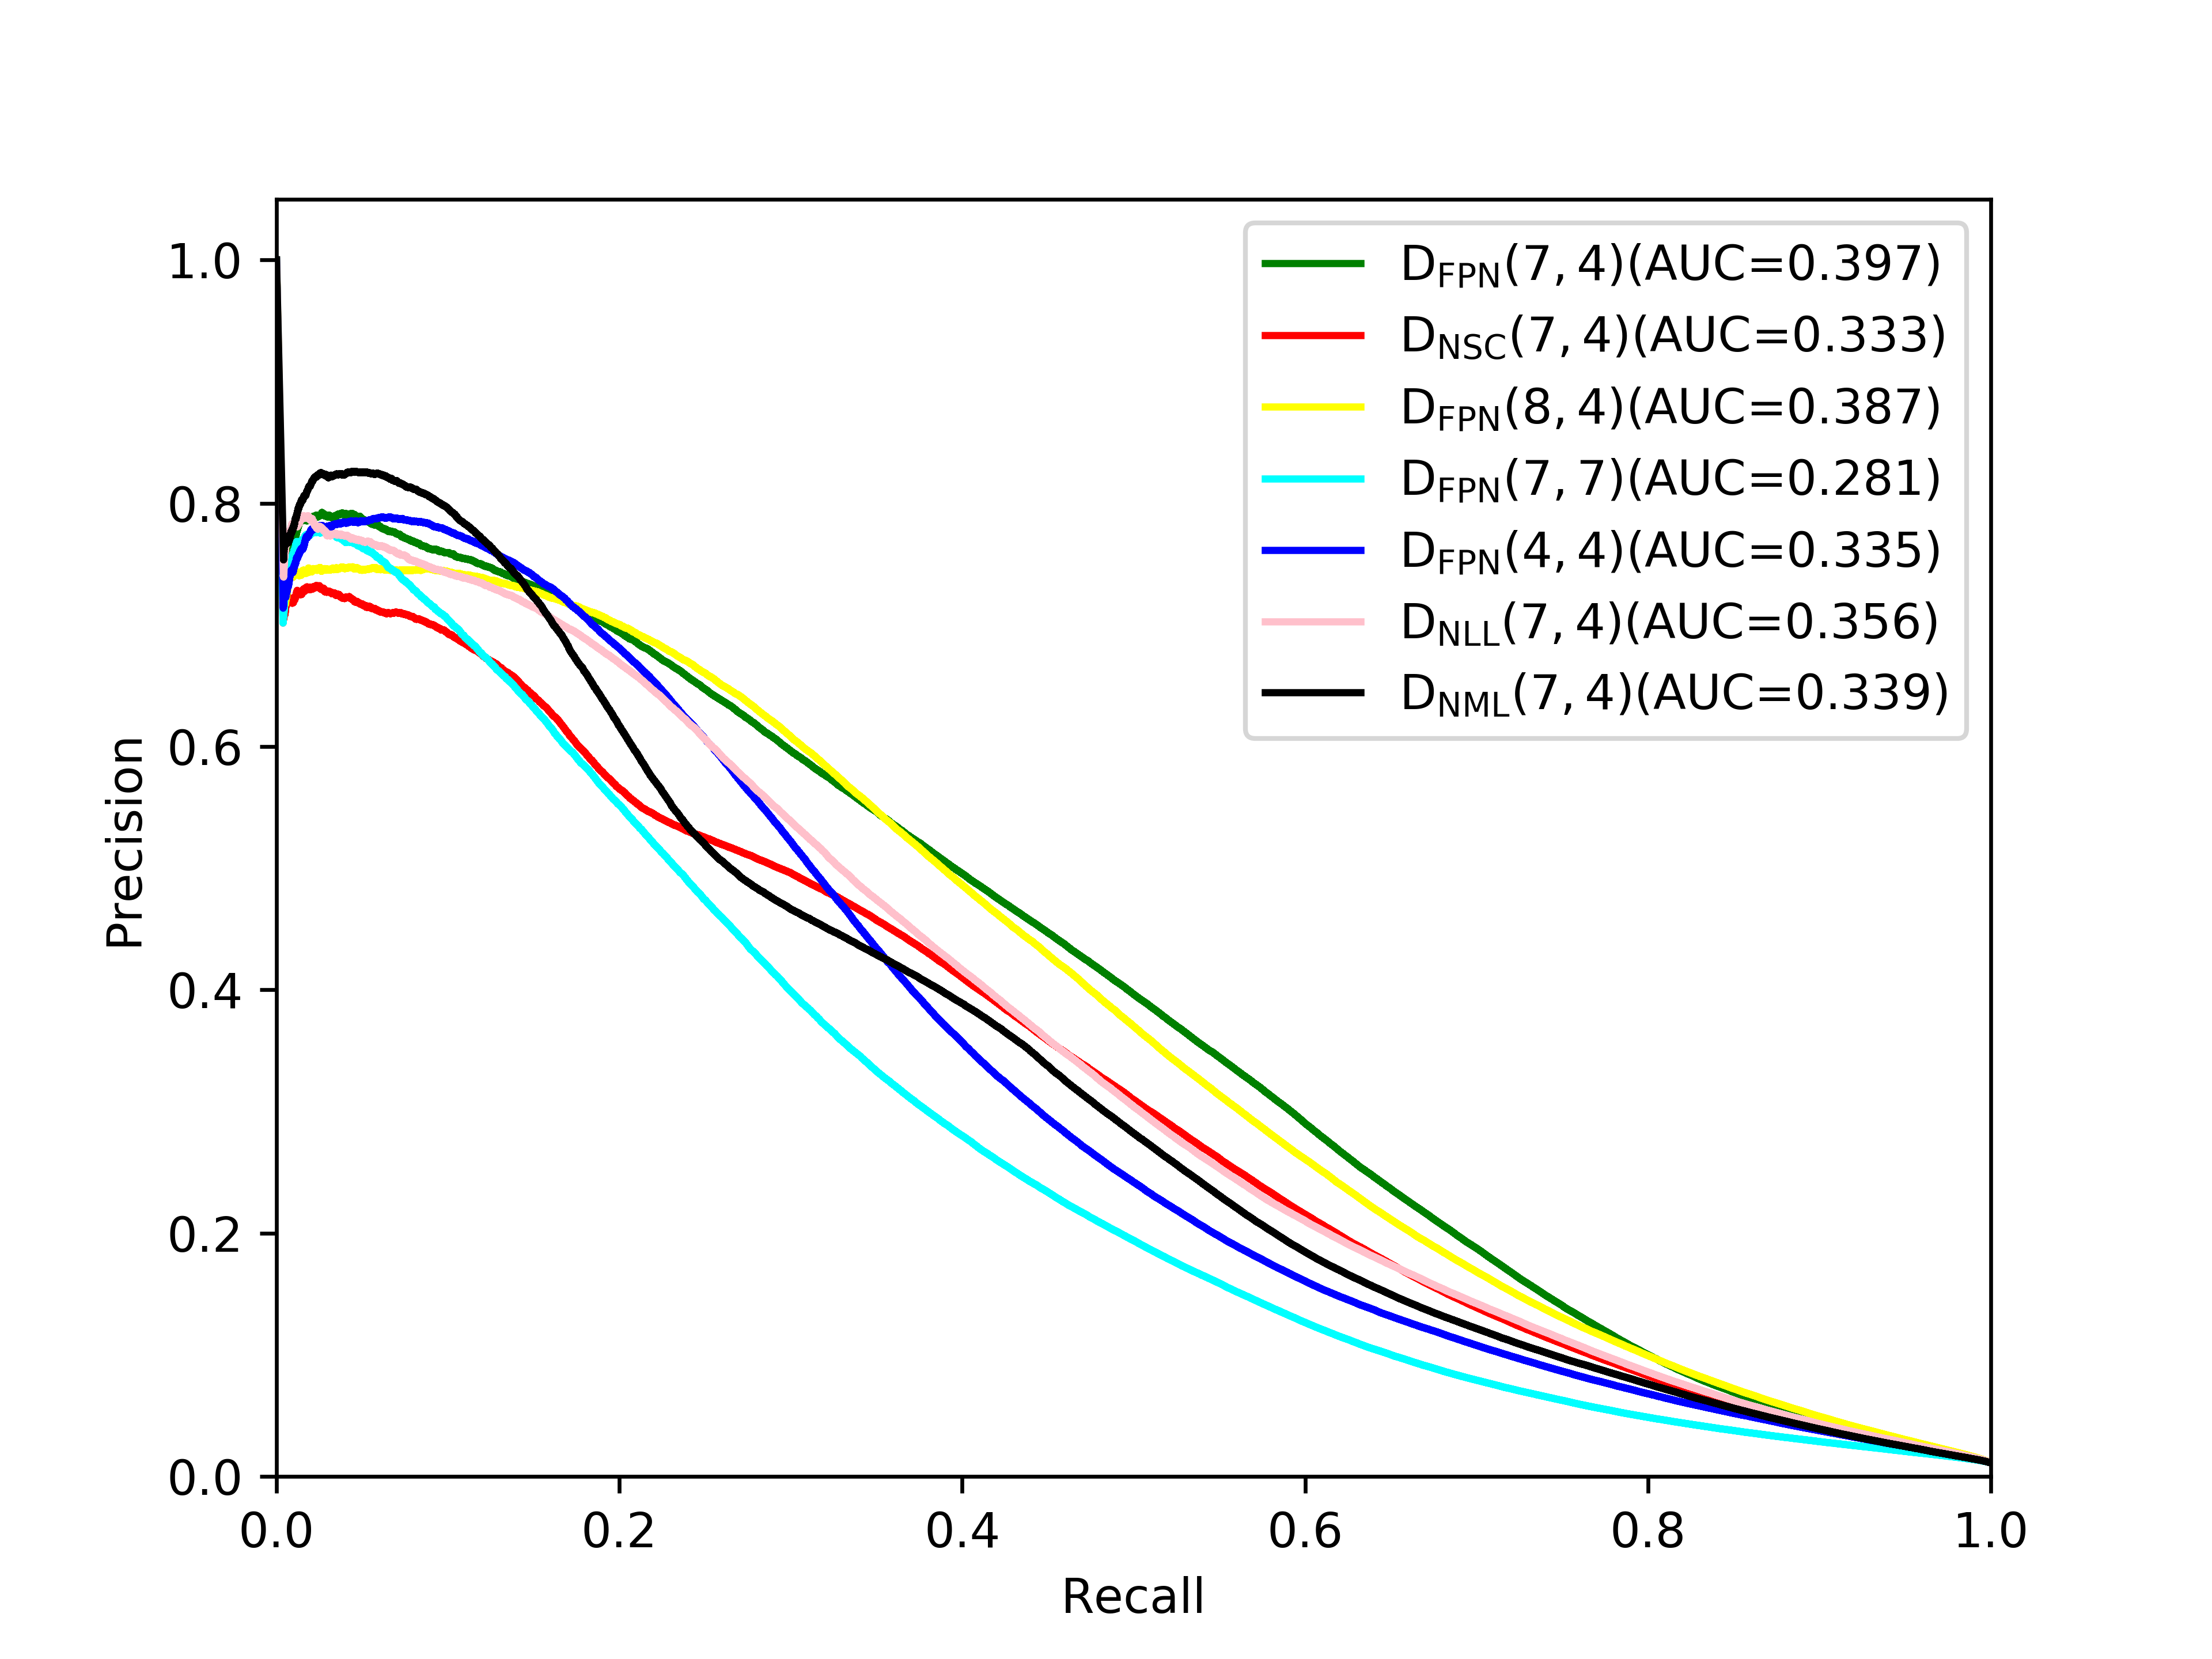
\includegraphics[width=1.0\textwidth]{figure/pr_curve_dis_arch/pr_curve.png}
	\caption{不同判别器模型结构下,本文提出的模型在二类模拟皮肤病病变数据集上得到的P-R曲线及其AUC(见右上角图例)。} 
	\label{fig:pr_curve_skin_dis_arch}
\end{figure}

从上图可以看出,对于默认判别器模型$\mathrm{D}_\mathrm{FPN}(7,4)$(图中绿色曲线),本文提出的模型定位性能最佳,AUC分数最高(AUC=$0.397$)。相比较之下,当去掉默认判别器所有跨层连接时($\mathrm{D}_\mathrm{NSC}(7,4)$,图中红色曲线),性能下降最为严重($0.397\rightarrow 0.333$),这主要是因为网络提取到的浅层高分辨率特征往往对异常图像中尺寸偏小的疾病标记物有着极强语义性。另外,在原始判别器基础上,我们去掉最后一个下采样单元与最后一个全连接层的跨层连接得到$\mathrm{D}_\mathrm{NML}(7,4)$(图中黑色曲线),同理,我们去掉第一个下采样单元与最后一个全连接层的跨层连接得到$\mathrm{D}_\mathrm{NLL}(7,4)$(图中粉色曲线),在以上两种情况下,虽然本文提出的模型的定位性能也有所下降,前者AUC:$0.397\rightarrow 0.339$,后者AUC:$0.397\rightarrow 0.356$,但是AUC分数的下降幅度与$\mathrm{D}_\mathrm{NSC}(7,4)$相比要小($\mathrm{D}_\mathrm{NSC}(7,4)$、$\mathrm{D}_\mathrm{NML}(7,4)$和$\mathrm{D}_\mathrm{NLL}(7,4)$相较于默认判别器模型,AUC分数下降幅度分别为$0.064$,$0.058$和$0.041$),也进一步说明判别器模型的浅层特征对于定位异常图像中分布广泛、大小不一的疾病标记物的重要性,这也是我们在判别器模型中加入跨层结构,让判别器融合不同层次、不同分辨率的特征的主要原因。另外,在默认判别器$\mathrm{D}_\mathrm{FPN}(7,4)$基础上再加入一个卷积单元可得到$\mathrm{D}_\mathrm{FPN}(8,4)$(图中黄色曲线),但就定位性能来看出现了略微下降(AUC分数为$0.387$),这是因为额外引入一个卷积单元虽然没有改变特征图的尺寸,但是对于尺寸较小的疾病标记物就来说,更深的网络意味着更低的语义性,梯度的回传也会变得相对困难。另外,本文针对判别器下采样的次数,本文也设置了相关实验,当判别器模型采用$\mathrm{D}_\mathrm{FPN}(7,7)$(图中青色曲线)时,我们发现本文提出的模型的定位性能最差(AUC=$0.281$)。由于输入图像尺寸为$128\times 128$,实际上判别器的下采样次数最多为$7$次,故随着下采样次数增加,特征图分辨率不断减少,在此过程中,相较于像素数量占绝对优势的正常像素,尺寸较小的疾病标记物的相关信息更难以被提取到,导致本该具备高语义的低分辨率高层特征对于尺寸较小的疾病标记物来说,其语义性大打折扣。反之,当下采样次数过少时,此时的“低分辨率”的高层特征中往往包含很多冗余或者无关干扰信息,故此时的高层特征的语义性也较低,这也是判别器模型采用$\mathrm{D}_\mathrm{FPN}(4,4)$(图中蓝色曲线)时,本文提出的模型的定位性能与默认判别器模型相比也有所下降的原因。而默认判别器模型中由于相比$\mathrm{D}_\mathrm{FPN}(4,4)$又有额外$3$个卷积单元,能过滤与疾病标记物无关的背景信息,增加了“低分辨率”高层特征的语义性,这也是采用默认判别器模型时本文提出的模型的定位性能更优的原因。为了更为直观看出以上各个模型之间的定位性能差异,我们将以上判别器模型结构及其AUC分数列在表\ref{tab:dis_arch}中。

\begin{table}[h]
	\centering
	\caption{不同超参数组合下,本文提出的模型在二类视网膜糖尿病病变数据集上计算得到的AUC分数列表。}		
	\label{tab:dis_arch}
	\resizebox{1.0\textwidth}{!}{
		\begin{tabular}{c|c|c|c|c|c|c|c}
			\toprule[2pt]
			& $\mathrm{D}_\mathrm{FPN}(7,4)$ & $\mathrm{D}_\mathrm{NSC}(7,4)$&
			$\mathrm{D}_\mathrm{NLL}(7,4)$&
			$\mathrm{D}_\mathrm{NML}(7,4)$& $\mathrm{D}_\mathrm{FPN}(8,4)$&
			$\mathrm{D}_\mathrm{FPN}(7,7)$&
			$\mathrm{D}_\mathrm{FPN}(4,4)$ \\
			\midrule[2pt]
			AUC	& $\textbf{0.397}$ &	$0.333 $ & $0.356$ & $0.339$ & $0.387$& $0.281$ & $0.335$	 \\
			\bottomrule[2pt]
		\end{tabular}
	}
\end{table}

\section{不同超参数下的实验结果分析}\label{sec:hyper_paras}
为了验证本文提出的模型的超参数鲁棒性(损失函数见等式\ref{equ:model_loss_func}),本文对损失函数中的两个超参数$\lambda_{1}$和$\lambda_{2}$进行测试,旨在找出比较鲁邦的超参数范围。为此,在保证学习率、迭代次数、网络参数初始化等所有相关设置相同的情况下,本文取了$7$种不同的$\lambda_{1}$和$\lambda_{2}$超参数取值,在二类糖尿病病变数据进行了相关测试。这里同样使用P-R曲线及其AUC分数作为评价标准。相关实验结果如图\ref{fig:pr_curve_retinal_hyper_paras}所示。

\begin{figure}[h]
	\centering
	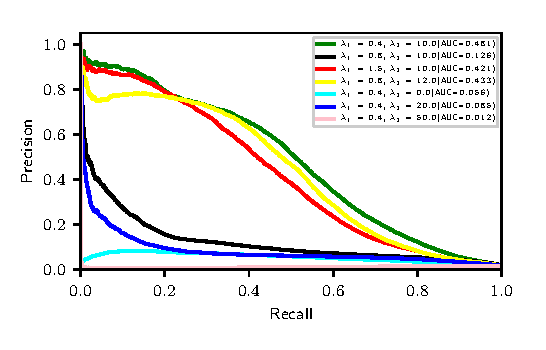
\includegraphics[width=1.0\textwidth]{figure/pr_curve_retinal_hyper_paras/pr_curve.eps}
	\caption{不同超参数$\lambda_{1}$和$\lambda_{2}$组合下,本文提出的模型在二类糖尿病病变数据集上得到的P-R曲线及其AUC(见右上角图例)。} 
	\label{fig:pr_curve_retinal_hyper_paras}
\end{figure}

从图\ref{fig:pr_curve_retinal_hyper_paras}可以看出,在$\lambda_{1}=0.4, \lambda_{2}=10$、$\lambda_{1}=1.5,\lambda_{2}=10$和$\lambda_{1}=0.8,\lambda_{2}=12$这三组超参数设置下,模型性能表现比较稳定,AUC取值分别为$0.481$(图中绿色曲线)、$0.421$(图中红色曲线)和$0.433$(图中黄色曲线)。说明$\lambda_{1}\in [0.4,1.5]$,$\lambda_{2}\in [10,12]$范围内,文本提出的模型的性能比较稳定。另外,注意到$\lambda_{1}=0.4,\lambda_{2}=0$时,本文模型取得较低AUC($0.056$,图中青色曲线),说明损失函数中L1损失对编码器-解码器输入输出约束的必要性(见等式~\ref{equ:model_loss_func})。而当$\lambda_{2}\geq 20$时,本文提出模型的性能也比较差,其中,$\lambda_{2}=20$时,AUC为$0.085$(图中蓝色曲线);$\lambda_{2}=50$时,AUC为$0.012$(图中品红色曲线),这主要是因为当$\lambda_{2}$过大时,在损失函数中真正起主导作用的是L1损失函数,此时,无论对于异常图像还是正常图像输入,编码器-解码器模块的输入输出均变化不大,从而导致疾病标记物定位失败,表现出AUC较低,比较接近基准模型(相关叙述见\ref{sec:g_c_g_d_g_d_c_comparsion}小节)的定位性能。而另一个极端,当$\lambda_{1}\rightarrow 0$时,相当于模型中移去CNN分类器,相关结果在\ref{sec:g_c_g_d_g_d_c_comparsion}小节中已有展示。另外,为了更为直观的观察不同超参取值下的模型性能,本文将超参数组合与对应AUC分数列在表\ref{tab:diff_parameters}中。

\begin{table}[h]
	\centering
	\caption{不同超参数组合下,本文提出的模型在二类视网膜糖尿病病变数据集上计算得到的AUC分数列表。}		
	\label{tab:diff_parameters}
	\resizebox{1.0\textwidth}{!}{
		\begin{tabular}{c|c|c|c|c|c|c}
			\toprule[2pt]
			& $\lambda_{1}=0.4,\lambda_{2}=10$ & $\lambda_{1}=0.8, \lambda_{2}=10$& $\lambda_{1}=1.5, \lambda_{2}=10$&
			$\lambda_{1}=0.4,\lambda_{2}=0$& $\lambda_{1}=0.4,\lambda_{2}=20$ & $\lambda_{1}=0.4,\lambda_{2}=50$ \\
			\midrule[2pt]
			AUC	& $\textbf{0.481}$ &	$0.421 $ & $0.433$ & $0.056$ & $0.085$& $0.012$	 \\
			\bottomrule[2pt]
		\end{tabular}
	}
\end{table}

\section{本章小结}
本章主要展示了在二类模拟皮肤病病变数据集和二类视网膜糖尿病病变数据集上的相关实验结果及其分析,与CAM和Grad-CAM,从P-R曲线及其AUC角度看,本文提出的模型可以实现更为精确的疾病标记物定位结果。另外,为了让读者更清楚地理解本文提出的模型的内部情况,本章设计了系列消融实验,例如在\ref{sec:g_c_g_d_g_d_c_comparsion}小节中通过分别去掉CNN分类器和判别器的方式来探究二者在完整模型中所起到的作用。除了直接与CAM和Grad-CAM作比较来证明本文提出的模型的性能优越性,还通过间接方式分别从CNN分类器和判别器进行了进一步验证(参加\ref{sec:indirect_quantitative_evaluation}小节)。最后,还分别设计了两组对比实验分别探究了本文提出的模型的适用超参数范围和判别器结构变化对于整体模型的影响。在两个二类疾病标记物数据集上,相比于CAM和Grad-CAM,本章通过设计了一系列实验证明本文提出的方法在精确定位疾病标记物上的性能优越性。到此,本文提出的模型在二类疾病标记物的精确定位问题叙述完毕。接下来将在第\ref{sec:multi_classes}章中展示本文提出的模型在处理多类疾病标记物的精确定位问题的相关实验结果。如\ref{sec:existing_diffcuities}小节中所描述的那样,由二分类疾病标记物的定位问题到多分类疾病标记物的定位问题并不是一个简单的二类到多类的推广,而是存在诸多难题。在数据集方面,图像数量比较多、图像质量比较高的多类数据集难以收集,而且图像的像素级标注代价高昂的问题依然存在。在模型的训练方面,对于CNN分类器的处理比较容易,将二类交叉熵损失替换成多类交叉熵即可,难点是如何处理判别器,因为对抗生成网络只有正常/异常两个输入端,是否要添加新的判别器来处理新加入的类别,另外,存在多个类别时,如何组织数据训练模型,这些均是值得考虑的问题。接下来,在第\ref{sec:multi_classes}章中,本文将针对以上问题展开相关内容的叙述,同时选取可用于多类疾病标记物精确定位任务相关的数据集,最后展示相关实验结果并对其进行分析。



        %\newclearpage
        \chapter{多类生物标记物定位问题的实验评估}\label{sec:multi_classes}
\section{前言}
在上一章中,与包括CAM和Grad-CAM在内的两种可视化方法相比,本文介绍了我们提出的模型在处理二类生物标记物定位问题的优异表现。与上一章内容安排一样,在本章中,我们将本文提出的模型由二类问题推广到多类问题,并展示相关实验结果与分析。首先在\ref{sec:mul_classes_ds_intro}小节中,本文将会介绍实验数据集的相关信息。在\ref{sec:multi_classes_experiment_setting}小节中,本文将会说明实验相关设置,包括学习率、实验超参数、优化器等信息。从\ref{sec:multi_classes_experiments_res}小节开始,本文将展示本文提出的模型在处理多类生物标记物定位问题上的相关实验结果,同样包括与CAM和Grad-CAM的相关对比实验和与判别器网络结构相关的消融实验,随后本文会在\ref{sec:multi_classes_hyper_paras}小节中对超参数组合进行相关测试。注意,由于本章实验相关评价标准与上一章完全一样,所以本章不再作相关赘述。下面展开本章内容的具体阐述。
\section{数据集介绍}\label{sec:mul_classes_ds_intro}
\subsection{多类模拟皮肤病病变数据集}
多类模拟皮肤病病变数据集同样是包含带有人工生物标记物的皮肤图像,图像尺寸大小均为$128\times 128$,图像均以PNG格式存储,每张图像不仅有图像级标注,还有像素级标注,故可用于定量分析有关的实验评估。在\ref{subsec:bin_simulated_skin_ds}小节中用到的二类模拟皮肤病病变数据集基础上额外增加了两类,故多类模拟皮肤病病变数据集中一共有$4$类,其中$3$类异常,$1$类正常。正常类图像是从ISIC2018~\cite{codella2019skin, tschandl2018ham10000}分类任务中的图像\footnote{https://challenge2018.isic-archive.com/task3/}通过滑动窗口方式收集$922$张正常皮肤图像(实际上是图像块)。第一类异常与二类模拟皮肤病病变数据集中的异常类一样,生成过程也相同(相关介绍参见\ref{subsec:bin_simulated_skin_ds}小节)。第二类异常图像中的生物标记物是黑色素瘤病变区域,为了生成这个数据集,我们首先从ISIC2018的分类任务(注意没有重复使用图像)提取了图像大小为$128\times 128$的正常图像(同样通过滑动窗口方式)。同时,我们根据ISIC2018的分割任务\footnote{https://challenge2018.isic-archive.com/task1/}中的黑素瘤区域的像素级标签,将其中的黑素瘤像素提取出来并嵌入到正常图像中。在此过程中,为了模拟真实皮肤图像中生物标志物的数量、大小和所在位置的随机变化,我们通过随机参数控制,在每个模拟皮肤图像的一定范围内随机生成这些参数的值。具体来说,黑色素瘤病变区域尺寸大小为$8\times 8$、$10\times 10$、$15\times 15$、$20\times 20$或者$25\times 25$。另外,为了产生不规则形状的生物标记物,对于每个缩略图的每个像素,以$1/3$概率不填充黑色素瘤像素。另外,我们还设置每张正常图像中嵌入的缩略图的数量不同($1$到$3$张不等)。第三类异常图像与第一类异常图像生成方法相同,只是第三类异常图像中的生物标记物不再是Image-Net图像的缩略图,而是圆环。注意,为了让三类模拟生物标记物的真实性,我们同样对第三类异常图像进行局部模糊。最终,正常类、第一、二、三类异常中分别有$922$、$1,310$、$1,051$、$1,062$张样本。该数据集中的部分图像示例如图\ref{fig:mul_classes_simulated_ds}所示。
\begin{figure}[h]
	\centering
	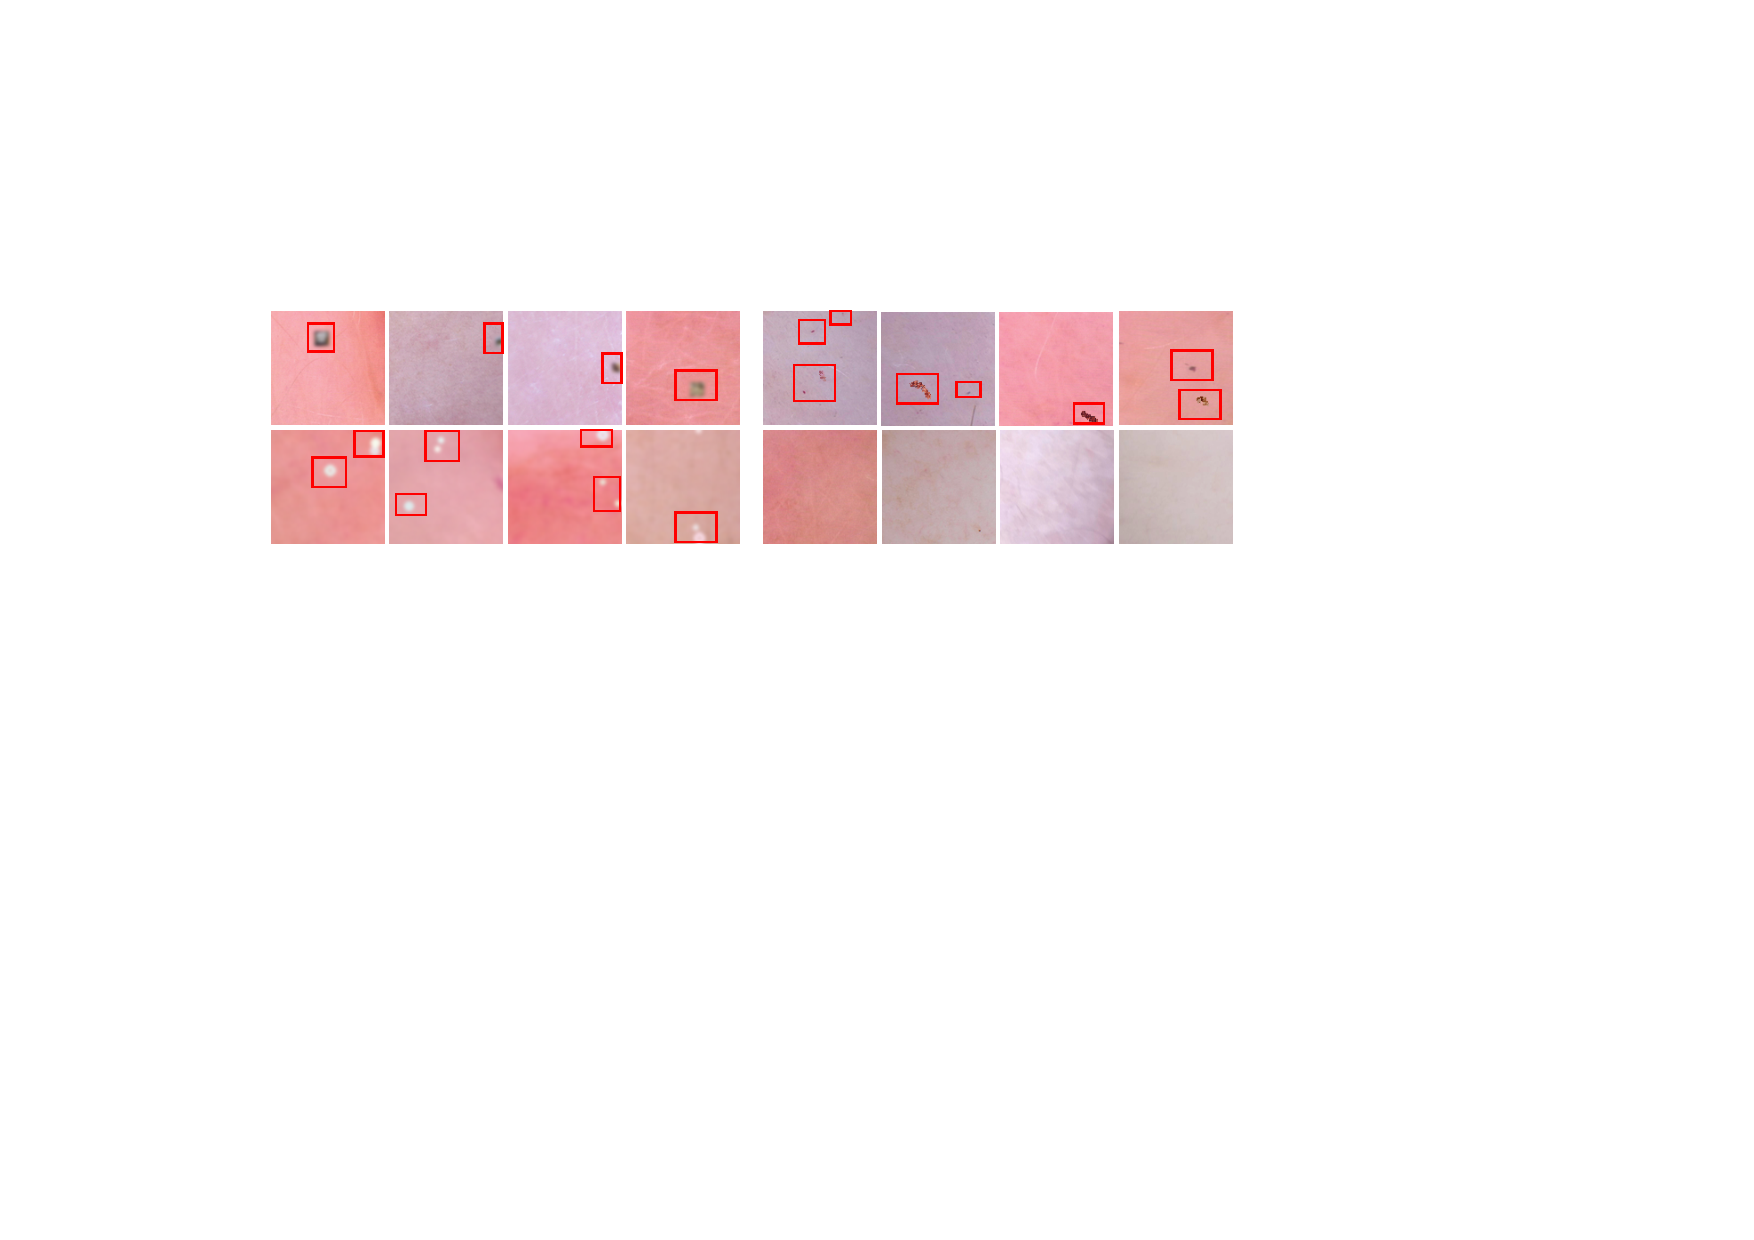
\includegraphics[width=1.0\textwidth]{figure/multi_classes_simulated_skin.pdf}
	\caption{多类模拟皮肤病病变数据集图像示例:按照从上到下,从左到右的顺序,第$1$行第$1$列到第$1$行第$4$列为皮肤图像加上经过局部模糊的Image-Net缩略图的异常图像(第一类异常);第$1$行第$5$列到第$1$行第$8$列为皮肤图像加上黑色素瘤区域的异常图像(第二类异常);第$2$行第$1$列到第$2$行第$4$列为皮肤图像加上经过局部模糊的圆环区域的异常图像(第三类异常);第$2$行第$5$列到第$2$行第$8$列为正常图像。异常图像中的生物标记物均已用红色矩形框标出。}
	\label{fig:mul_classes_simulated_ds}
\end{figure}

\section{实验设置}\label{sec:multi_classes_experiment_setting}
与上一章中二类问题所采用的相关实验设置相比,除超参数取值($\lambda_{1}=4.0,\lambda_{2}=20.0$)不同外,其他设置均相同。评价标准也与上一章相同(参见\ref{sec:exper_evaluation_metrics}小节),采用P-R曲线(多类模拟皮肤病病变数据集中三个异常类的像素数量统计表如\ref{tab:multi_ds_pixel_freqs}所示)作为实验评价标准。

由于对抗生成网络中只有两个语义输入端(真/假),与二类问题不同的是,多类问题有多个异常类。为了解决这个多类异常与对抗生成网络本身性质的矛盾,我们将所有异常类看做一类,而正常类本身就作为另一类,从而将正常类看做对抗生成网络语义上的真,将所有异常图像看做对抗生成网络语义上的假。同时,取样时保持所有异常类之间的样本数量相等。在CNN分类器方面,我们直接将原来的二分类扩展到多分类,增加CNN分类器最后一个全连接层的输出维度,同时在训练CNN分类器时用多类交叉熵取代原来的二类交叉熵损失函数。在判别器方面,由于多类模拟皮肤病病变数据集中的图像背景相对比较简单,高分辨率的浅层特征的也有较好的语义性。因此,在处理二类问题的判别器网络结构基础上(网络结构参见图\ref{fig:discrimintor_architecture},我们将用第二个下采样模块到最后一层的跨层连接替换掉了最后一个下采样模块到最后一层的跨层连接,让浅层特征更多的参与到最后一层全连接层的特征融合中。除此之外,本文提出模型的其他结构均与上一章相同。

\begin{table}[h]
	\centering
	\caption{多类模拟皮肤病病变数据集中的三类异常图像像素数量统计表。}
	\label{tab:multi_ds_pixel_freqs}
	\begin{tabular}{c|c|c|c}
		\toprule[2pt]
		数据集名称 & 正常像素数量 & 异常像素数量 & 比例 \\
		\midrule[2pt]
		第一类异常&  $21,222,487$ & $240,553$ & $\simeq 88: 1$ \\ \hline
		第二类异常&  $17,129,210$ & $90,374$ & $\simeq 190: 1$ \\ \hline
		第三类异常 & $17,341,855$ & $57,953$ & $\simeq 299: 1$ \\
		\bottomrule[2pt]
	\end{tabular}
\end{table}

\section{在多类模拟皮肤病病变数据集上的实验评估}\label{sec:multi_classes_experiments_res}
本文将展示本文提出模型在多类模拟皮肤病病变数据集上的实验结果,本文提出的模型同样将与CAM和Grad-CAM共计两种用于卷积神经网络可视化方法作定性分析和定量分析。下面展开相关内容的具体阐述。

\begin{figure}[H]
	\centering
	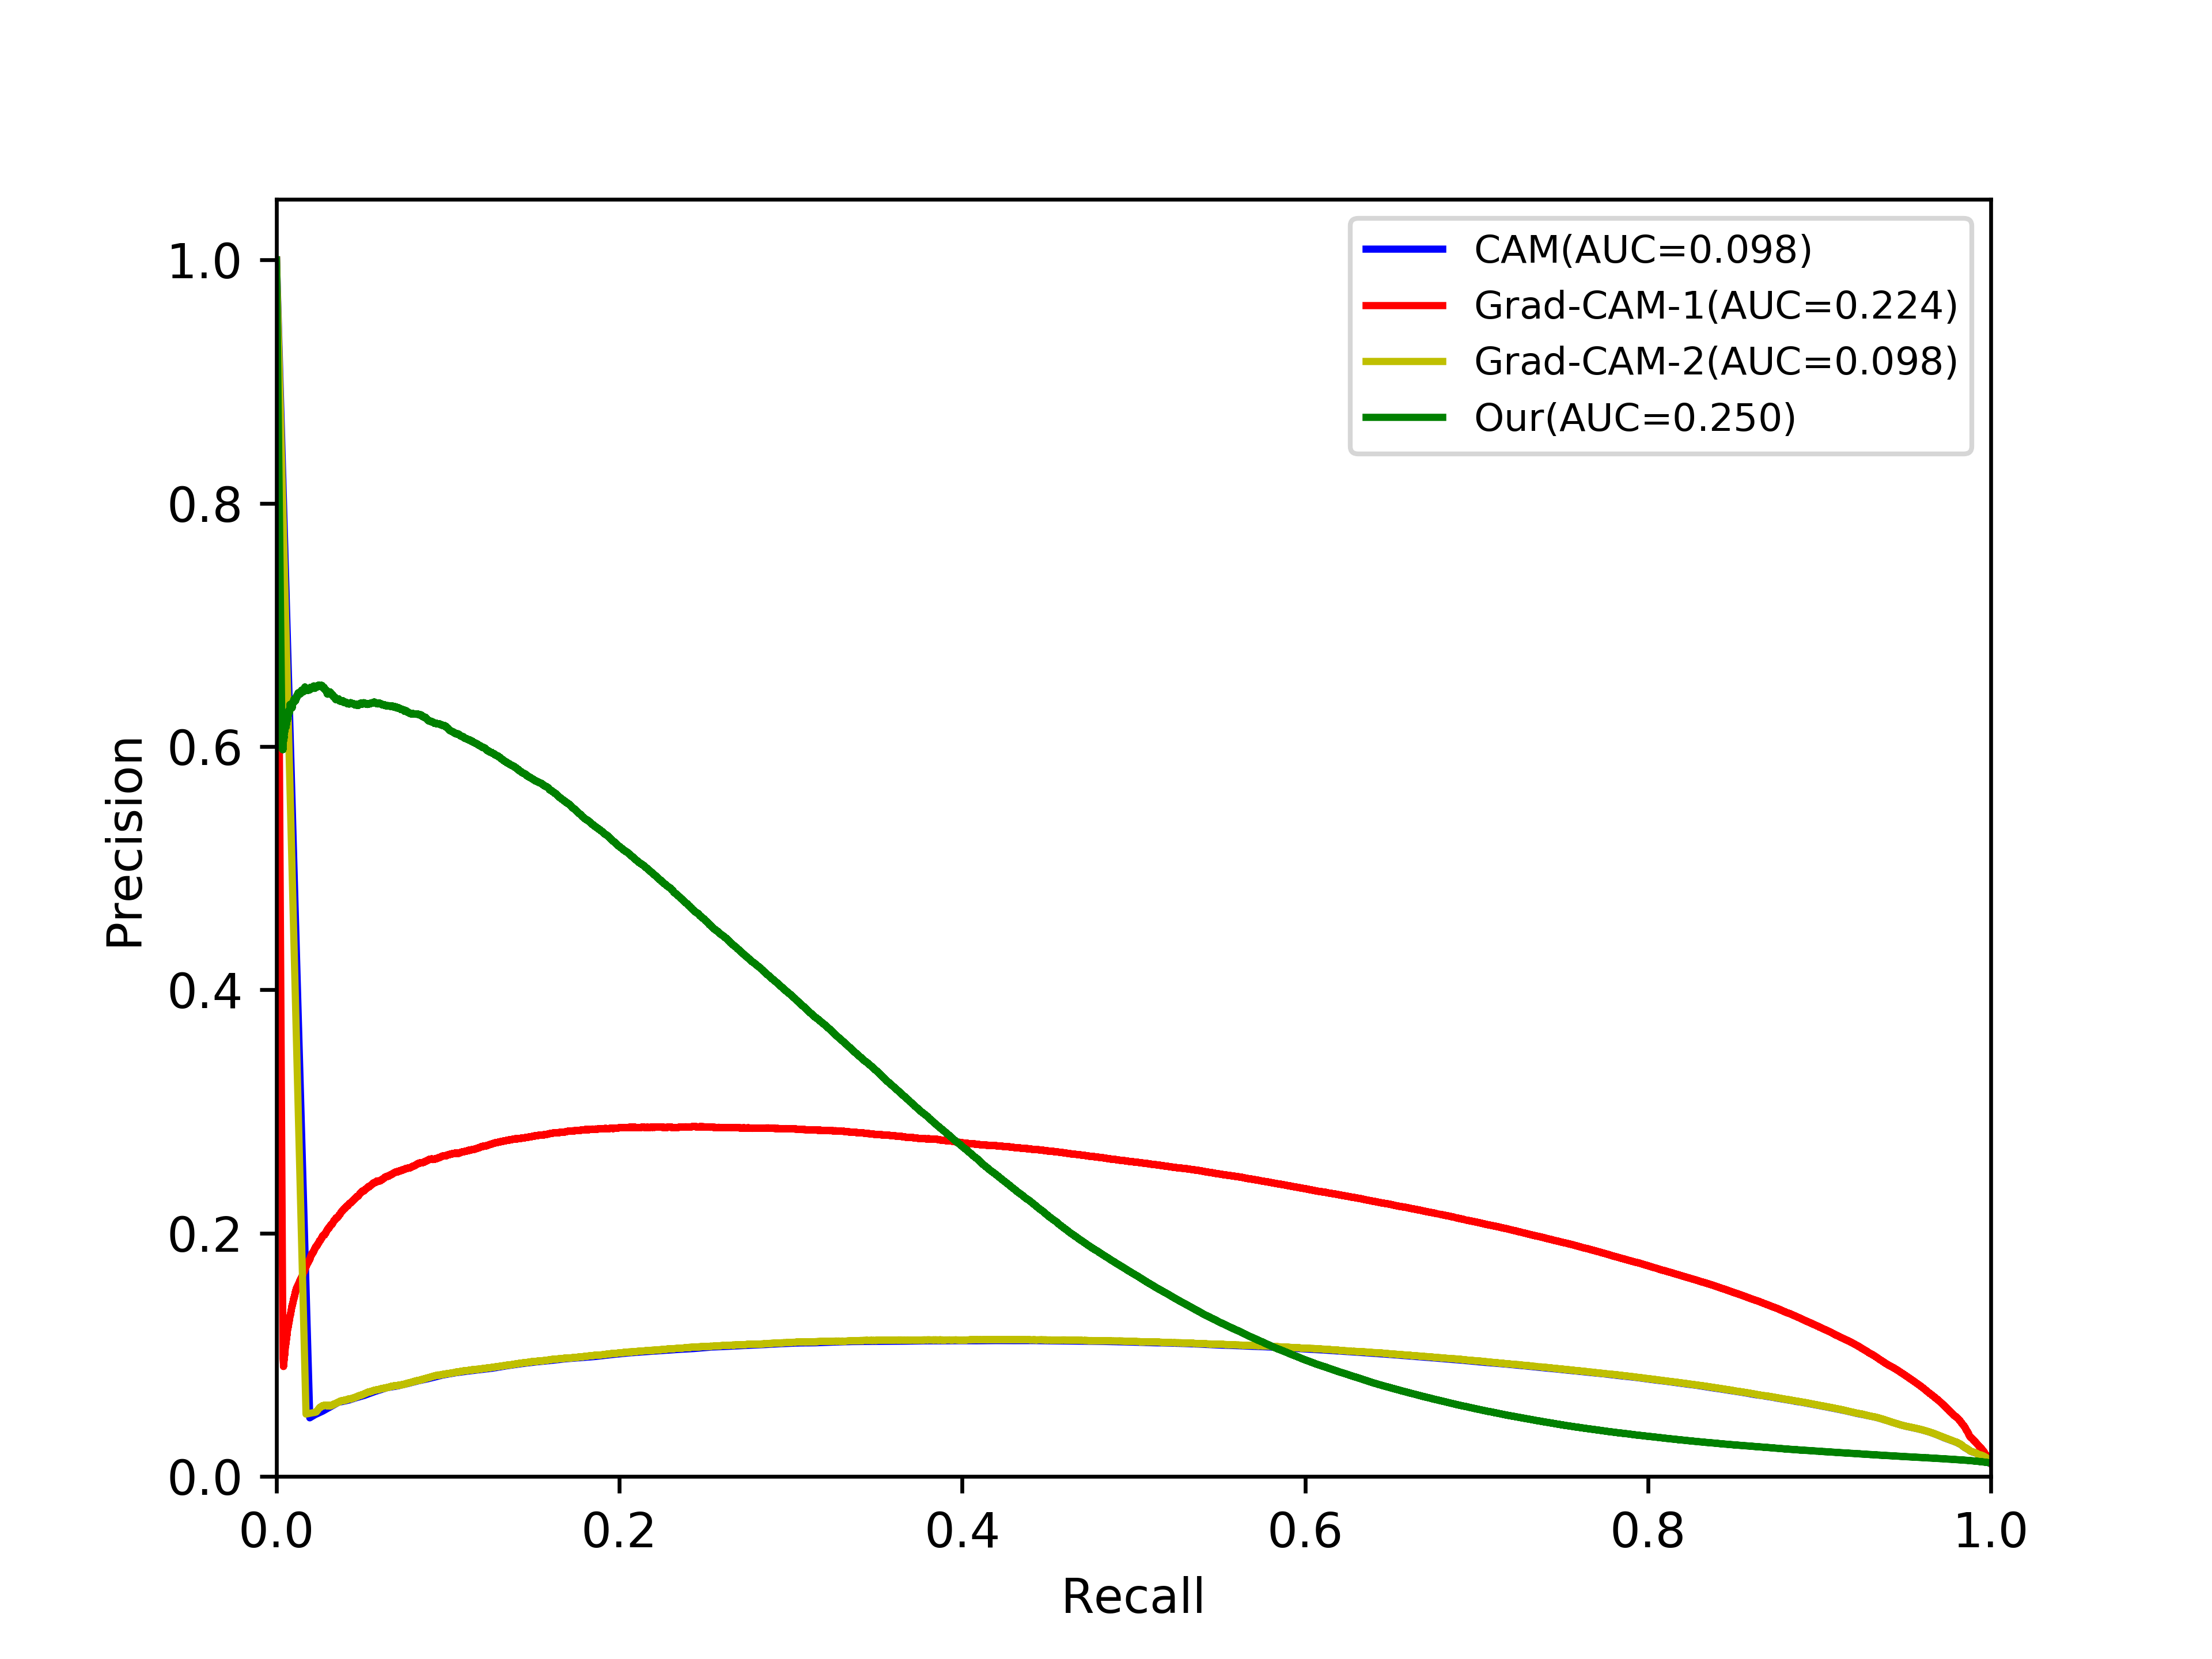
\includegraphics[width=1.0\textwidth]{figure/pr_curve_multi_skin/IMAGE_NET_pr_curve.png}
	\caption{CAM、Grad-CAM-1、本文提出的模型和Grad-CAM-2在多类模拟皮肤病病变数据集的第一类异常上画出的P-R曲线及其各自曲线下的面积(AUC,见右上角图例)。} 
	\label{fig:multi_simulate_pr_curve_image_net}
\end{figure}

\begin{figure}[H]
	\centering
	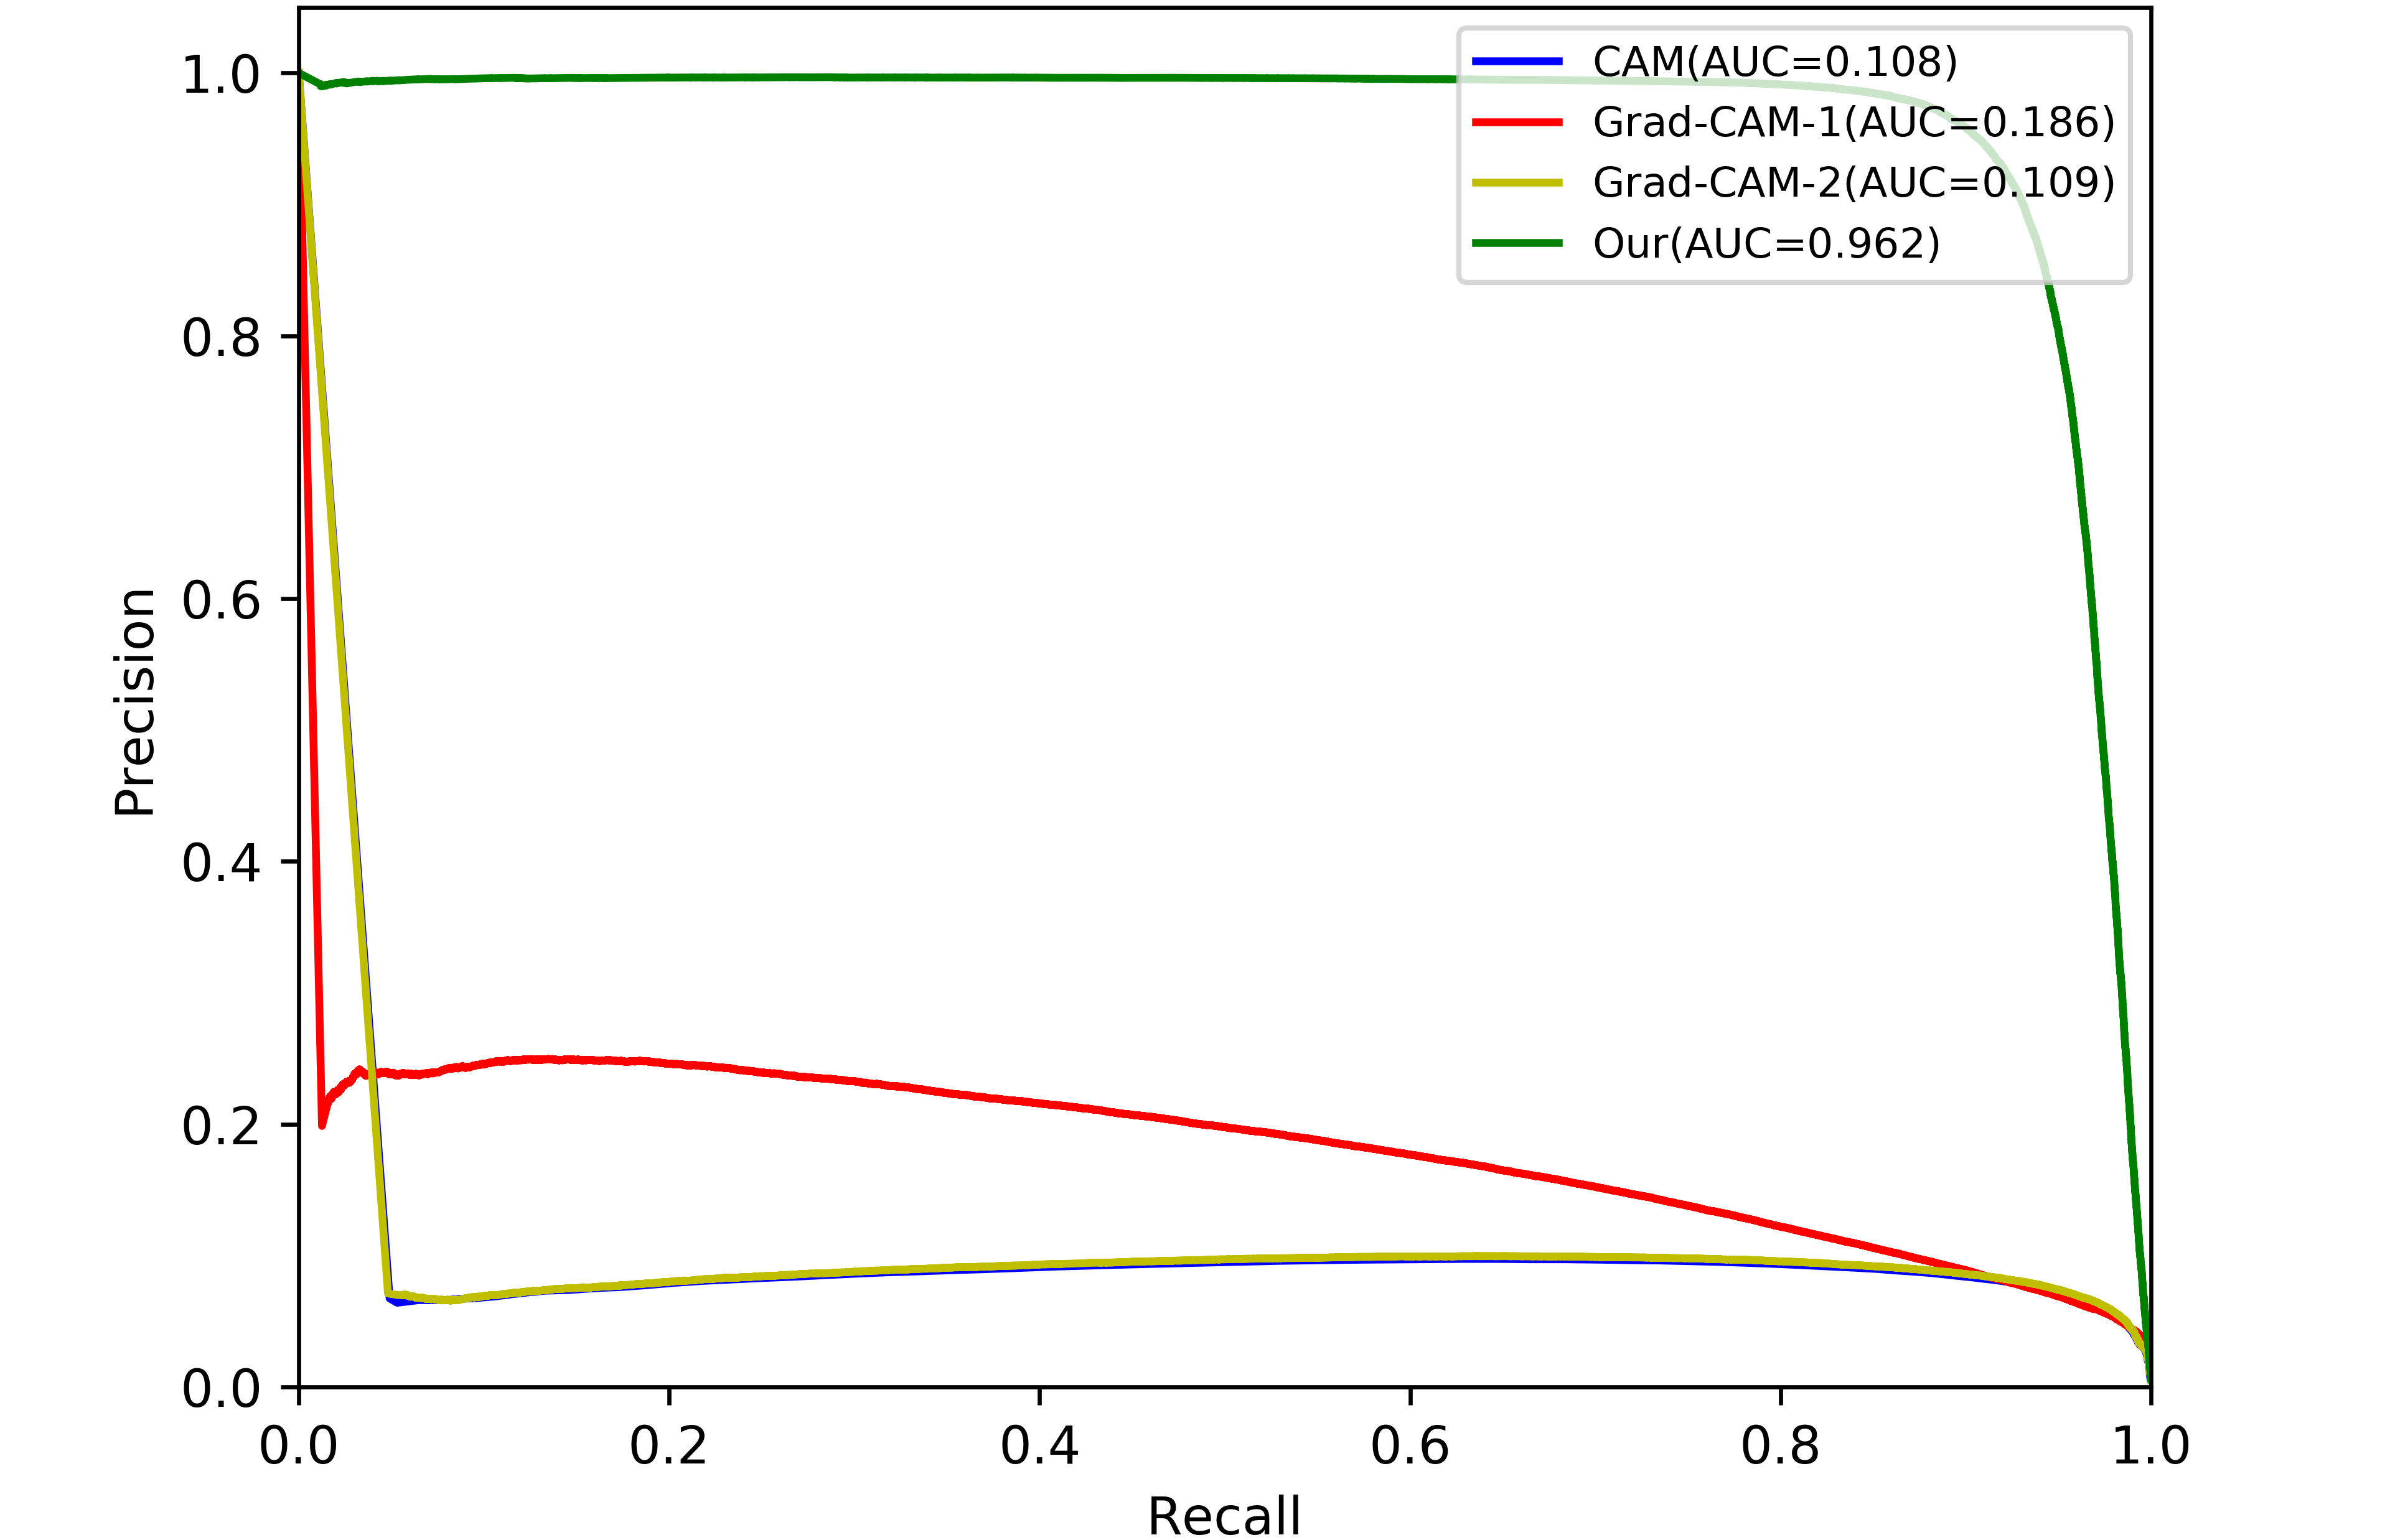
\includegraphics[width=1.0\textwidth]{figure/pr_curve_multi_skin/SKIN_pr_curve.png}
	\caption{CAM、Grad-CAM-1、本文提出的模型和Grad-CAM-2在多类模拟皮肤病病变数据集的第二类异常上画出的P-R曲线及其各自曲线下的面积(AUC,见右上角图例)。} 
	\label{fig:multi_simulate_pr_curve_skin}
\end{figure}
\vspace{-0.8cm}
\begin{figure}[H]
	\centering
	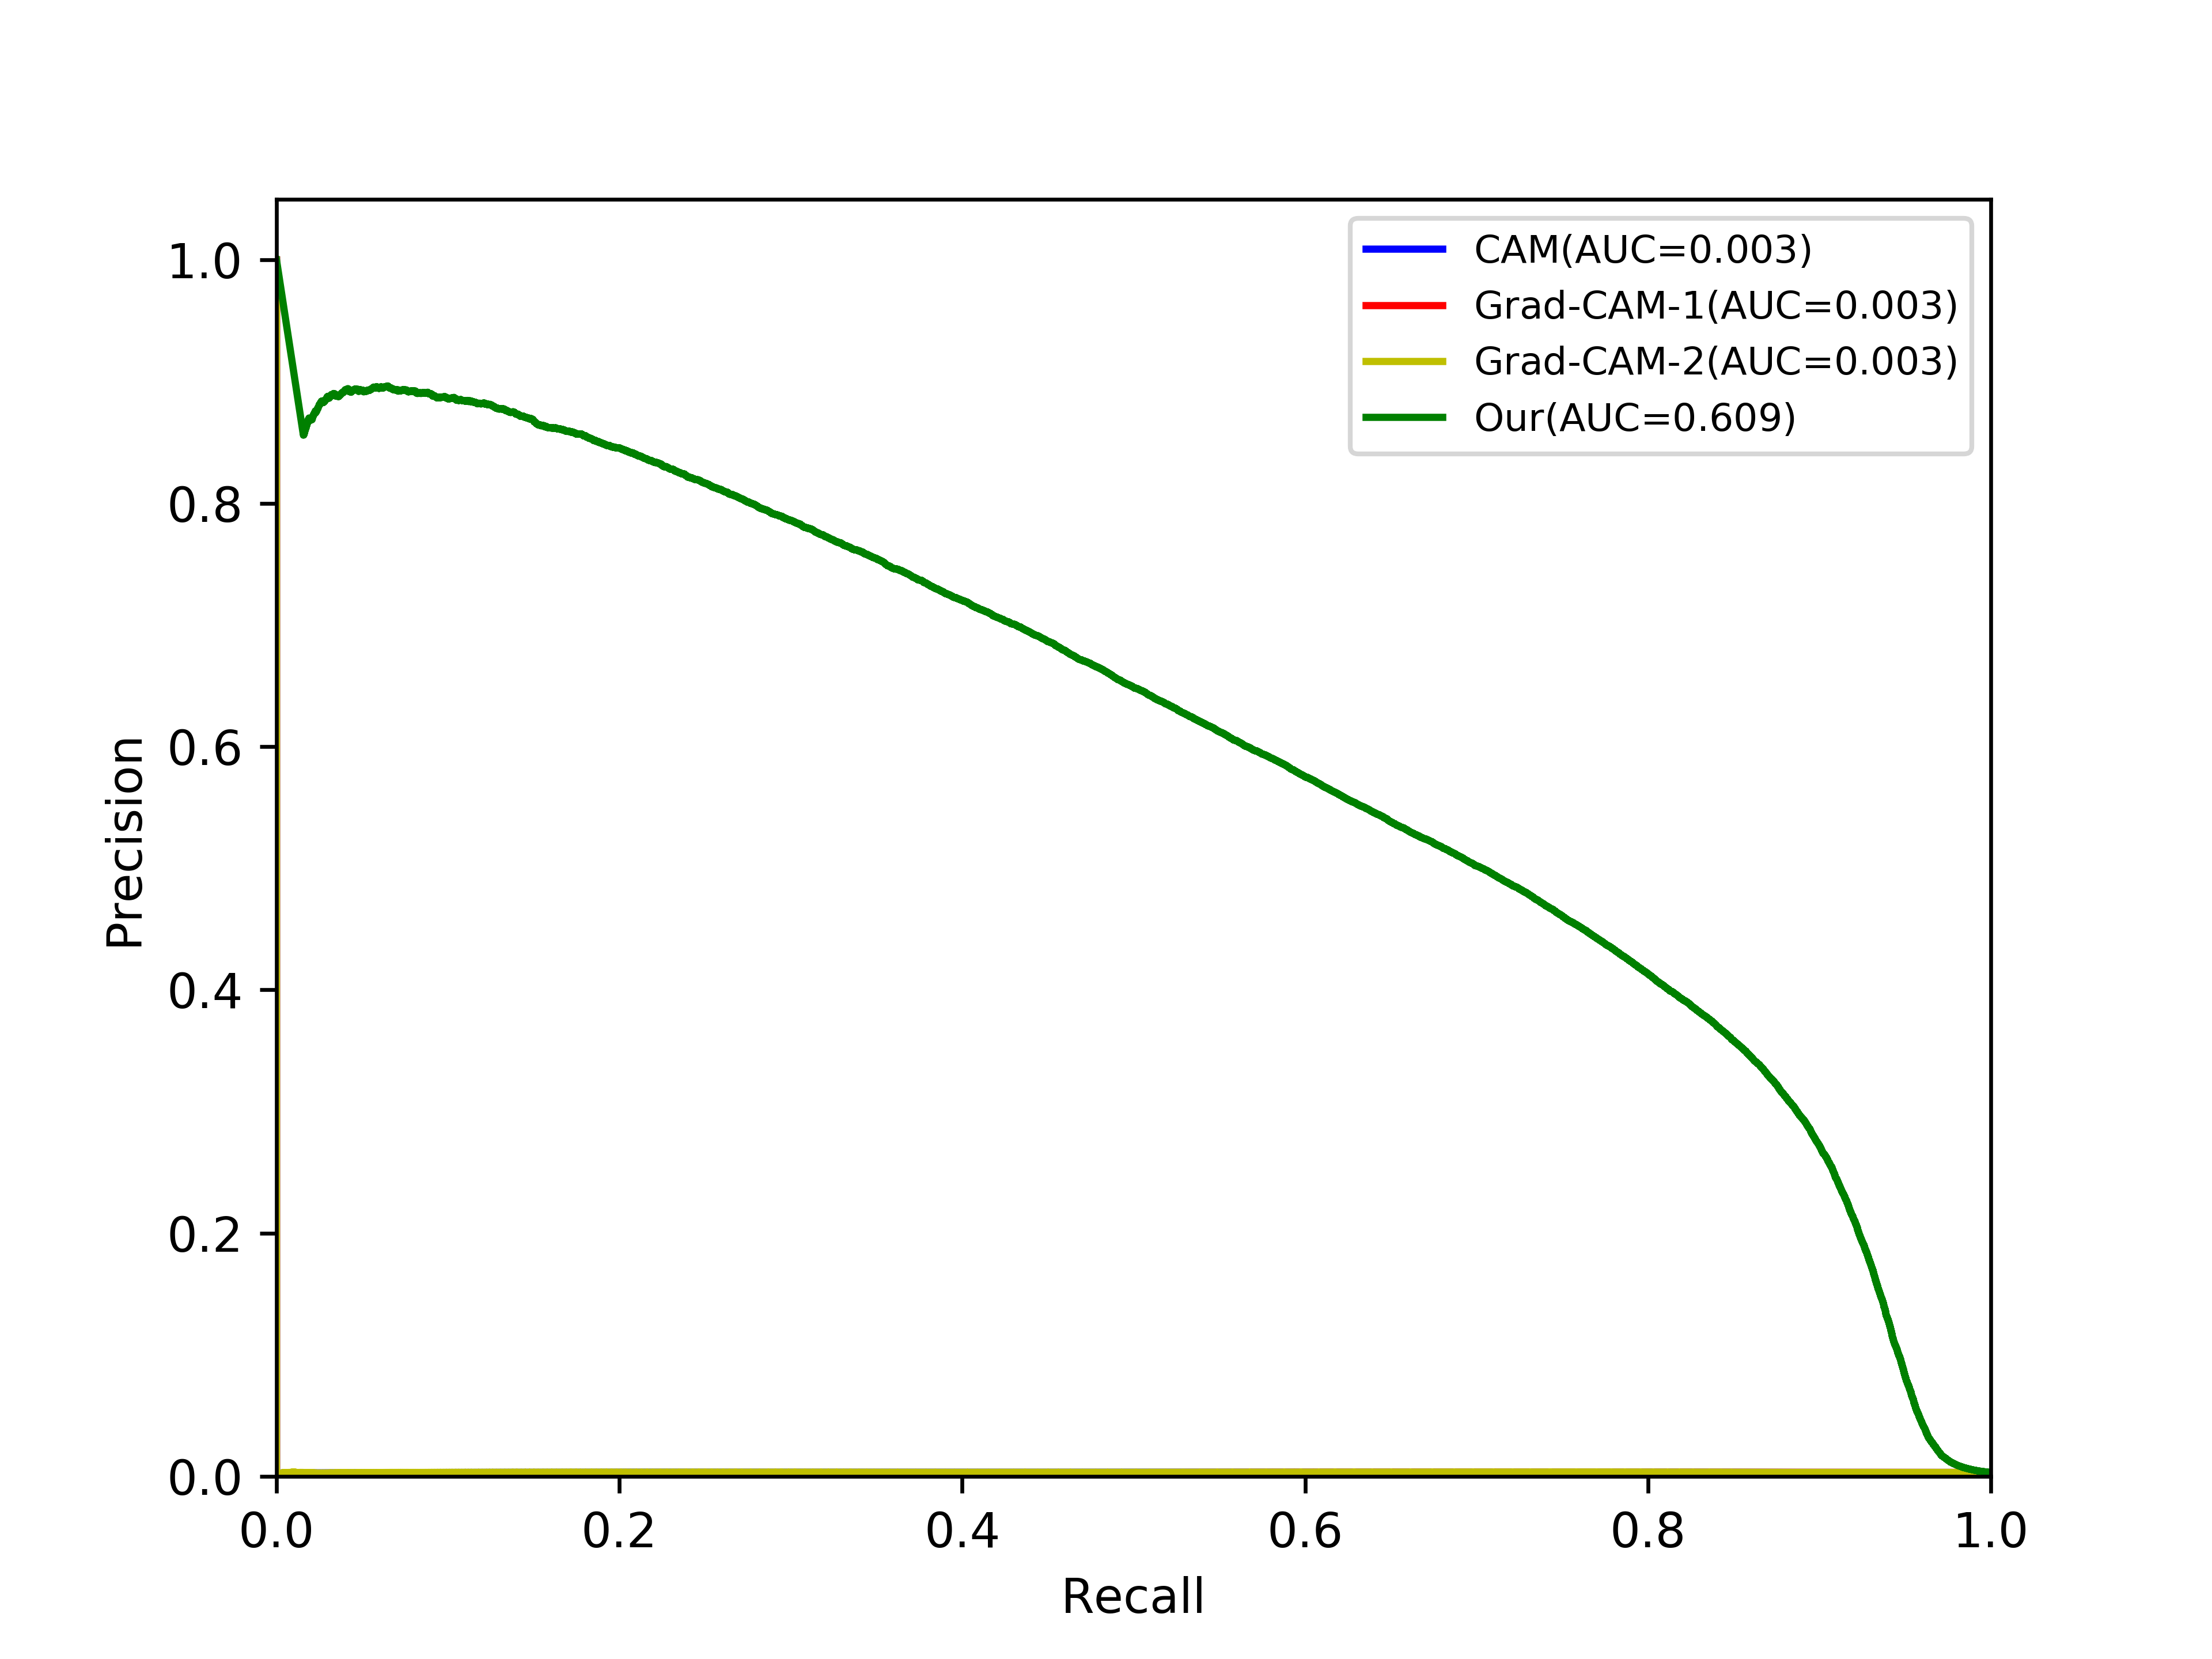
\includegraphics[width=1.0\textwidth]{figure/pr_curve_multi_skin/CIRCLE_pr_curve.png}
	\caption{CAM、Grad-CAM-1、本文提出的模型和Grad-CAM-2在多类模拟皮肤病病变数据集的第三类异常上画出的P-R曲线及其各自曲线下的面积(AUC,见右上角图例)。} 
	\label{fig:multi_simulate_pr_curve_circle}
\end{figure}


我们同样先训练得到了一个ResNet-18分类器,分类器最终的分类准确率达到了$99.9\%$,从而保证ResNet-18本身良好的分类性能。随后,与\ref{sec:bin_dr_ds_experiment}小节一样,我们分别使用CAM(见图\ref{fig:multi_simulated_skin_res}第$3$行)、Grad-CAM(见图\ref{fig:multi_simulated_skin_res}第$4$行和第$5$行)在多类模拟皮肤病病变数据集上完成了生物标记物的定位任务。
\begin{figure}[h]
	\centering
	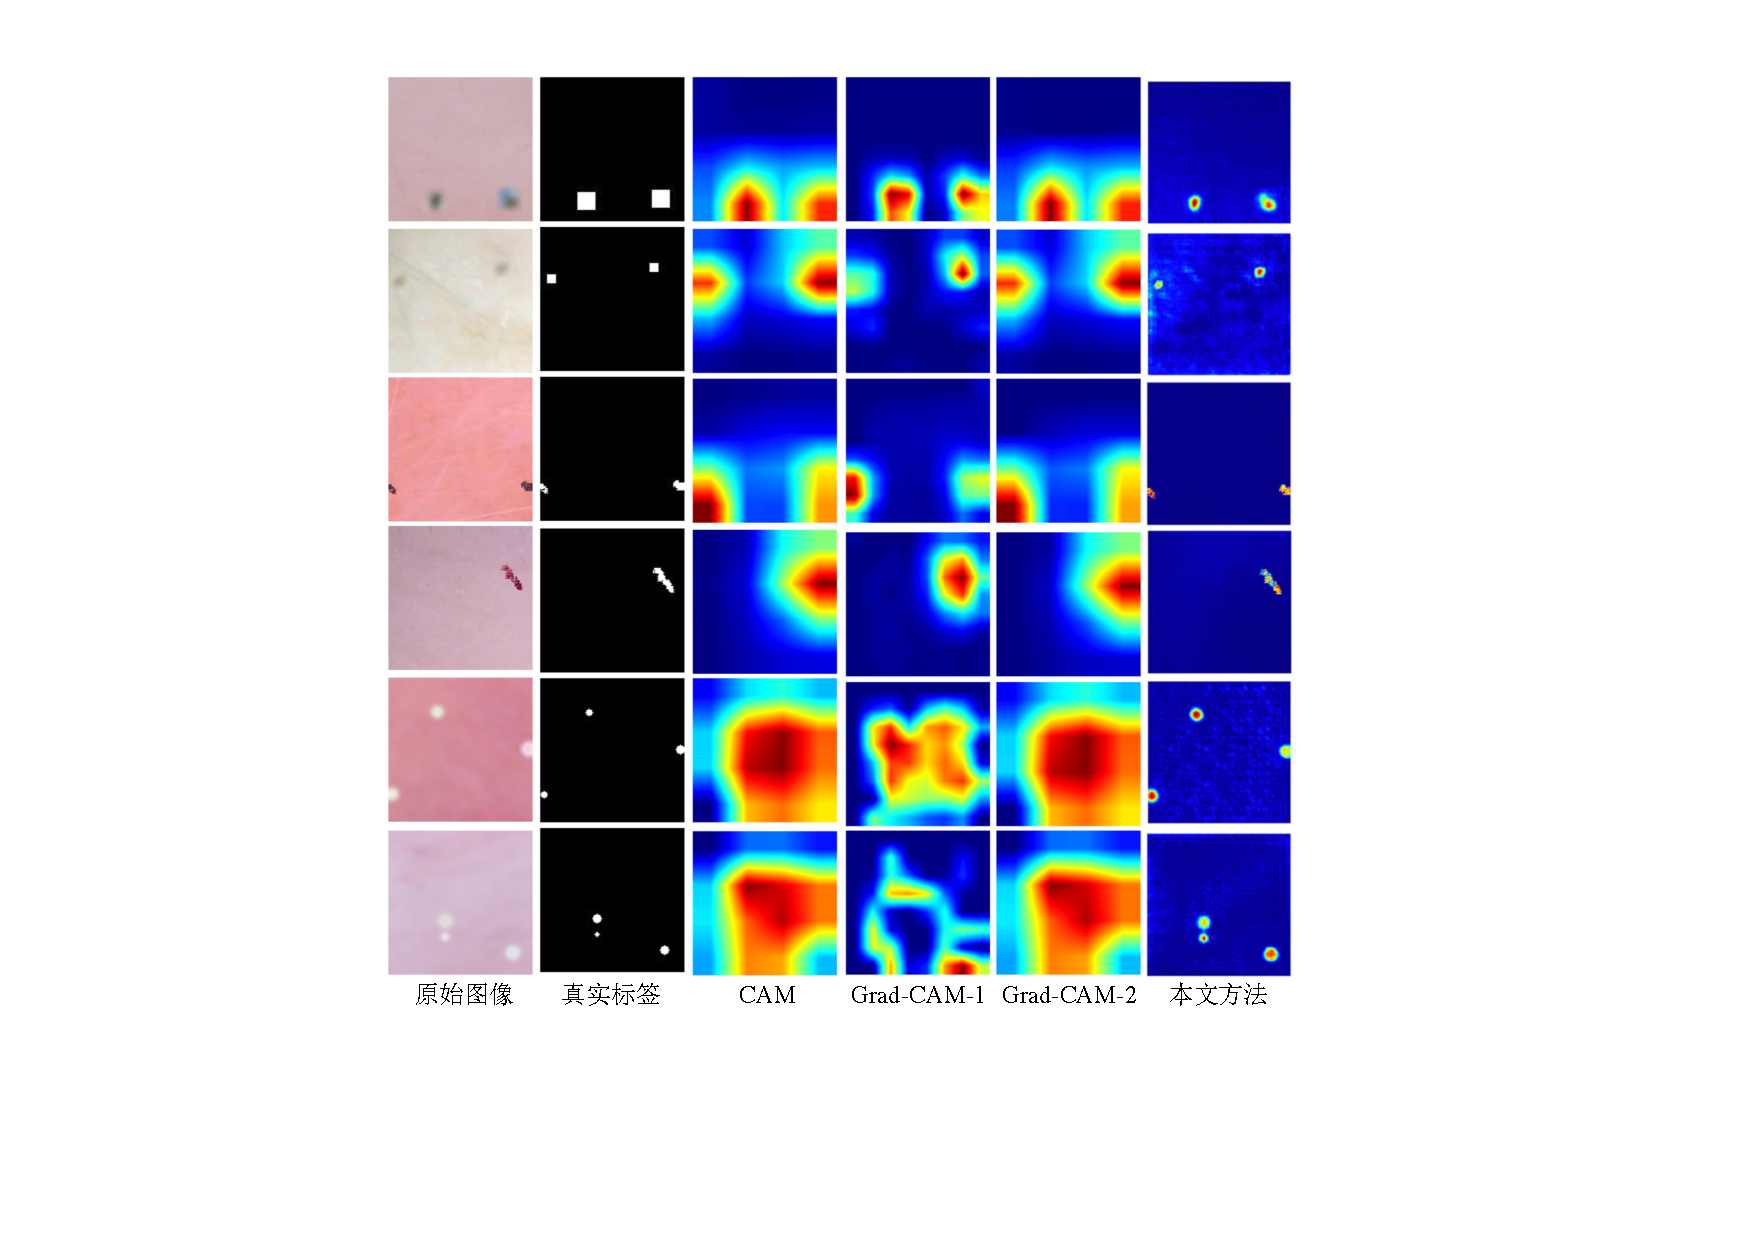
\includegraphics[width=1.0\textwidth]{figure/multi_simulated_skin_res.pdf}
	\caption{本文提出的模型在多类模拟皮肤病病变数据集上的定性评估:第$1-2$行、第$3-4$行和第$5-6$行分别为第一类异常、第二类异常和第三类异常图像实验结果。第$1$列表示该数据集中的原始图像,第$2$列表示原始的像素级标签。第$3$列表示CAM的定位结果,第$4$列表示Grad-CAM使用分类器中间层的特征图可视化结果(Grad-CAM-1),第$5$列表示Grad-CAM使用分类器最后一层特诊图可视化的定位结果(Grad-CAM-2),第$6$列表示本文提出模型的定位结果。}
	\label{fig:multi_simulated_skin_res}
\end{figure}

如图\ref{fig:multi_simulated_skin_res}所示,第$3$的定位结果标出的异常区域最多,虽然也包括了潜在的生物标记物,但是同时也将周边大量正常区域也误认作生物标记物。Grad-CAM作为CAM的扩展,对可视化层的选择更为灵活。如图中第$4$列和第$5$列分别选取中间卷积层和最后一层卷积层。可以发现,Grad-CAM-1取得了较为精确的结果,证明了其优于CAM的性能。另外,可以发现Grad-CAM-2给出的定位结果(第$5$列)与CAM(第$3$行)相差不大。与以上结果相比较,对于分散、形状各异的生物标记物,相比于CAM和Grad-CAM,本文提出的模型给出了更为精确的定位结果(第$6$行),从而从定性分析角度证明了本文提出的方法的性能优越性。


另外,由于多类模拟皮肤病病变数据集中的所有图像均存在像素级标注,本文还从定量角度对实验结果进行相关分析。由此,对于本文提出的模型、CAM、Grad-CAM-1和Grad-CAM-2,根据该数据集中的三类异常图像所绘制P-R曲线分别如图\ref{fig:multi_simulate_pr_curve_image_net}、图\ref{fig:multi_simulate_pr_curve_skin}和图\ref{fig:multi_simulate_pr_curve_circle}所示。不难发现,绿色P-R曲线(本文提出的方法)在其他三条曲线的上方,且与下侧横轴和左侧纵轴围成的封闭区域面积显然最大。在第一类异常、第二类异常和第三类异常上,本文提出的方法均取得了最高的AUC分数,在三类异常上计算得到的AUC分数分别为$0.236$(见图\ref{fig:multi_simulate_pr_curve_image_net})、$0.962$(见图\ref{fig:multi_simulate_pr_curve_skin})和$0.805$(见图\ref{fig:multi_simulate_pr_curve_circle}),从而从定量角度说明本文提出的方法相较于CAM和Grad-CAM具有更为出色的性能表现。以上四种方法更为直观的AUC分数如表\ref{tab:multi_ds_auc_scores}所示。

\begin{table}[!htbp]
	\centering
	\caption{本文提出的方法、CAM、Grad-CAM-1和Grad-CAM-2根据多类模拟皮肤病病变数据集中的三类异常图像计算得到的AUC分数及其平均值。}
	\label{tab:multi_ds_auc_scores}
	\begin{tabular}{c|c|c|c|c}
		\toprule[2pt]
		& CAM & Grad-CAM-1 & Grad-CAM-2 & 本文提出的方法 \\
		\midrule[2pt]
		第一类异常&$0.098$ & $0.224$ &  $0.098$ & $\textbf{0.236}$ \\ \hline
		第二类异常&  $0.108$ &$0.186$ & $0.109$ & $\textbf{0.962}$ \\ \hline
		第三类异常 & $0.003$ & $0.003$ & $0.003$ & $\textbf{0.805}$ \\ \hline
		Average AUC & $0.070$ & $0.138$ & $0.070$ & $\textbf{0.668}$ \\
		\bottomrule[2pt]
	\end{tabular}
\end{table}

\section{对于经过编码器-解码器的多类模拟皮肤病病变图像的定量分析}
在本节中,本文同样将设置一组实验从间接角度证明本文提出的模型能够较好去除异常图像中的生物标记物或者异常区域。与\ref{sec:indirect_quantitative_evaluation}小节中的设计思想相同,在理想情况下,如果一种方法能够完全定位并去除生物标记物,则去除生物标记物之后的图像不再包含生物标记物,则这些图像将很难与正常图像分开。根据以上前提假设,我们将多类模拟皮肤病病变数据集按照$80\%$和$20\%$的比例将其分为训练集和测试集(下文简称为“原始四类数据集”),随后用训练集训练一个ResNet-18四分类器。接着,我们将原始多类数据集中的每一张图像作为输入送入编码器-解码器,并将输出收集起来,这样我们得到一个新的数据集(下文简称为“‘正常’四类数据集”)。最后,我们用上述ResNet-18对“正常”多类数据集中的每一张图像进行分类。在评价标准方法,与\ref{sec:indirect_quantitative_evaluation}小节不同的是,我们不选定Recall和Specificity作为评价标准,这是因为多类问题中异常图像作为输入经过编码器-解码器之后的输出可能会向其他异常类转变而二类问题中异常图像作为输入经过编码器-解码器之后的输出只能向正常图像转变。因此,对于正常图像,我们希望编码器-解码器的输出中尽量少的图像被ResNet-18判别为异常;而对于异常图像,我们希望编码器-解码器的输出中尽量多的图像被ResNet-18判别为异常。因此,编码器-解码器对于正常图像输入的保持能力可定义为:

\begin{equation}\label{equ:normal_imgs_kep_rate}
\text{正常类的转化率}=\frac{\text{输出图像中被判定为异常的图像数量}}{\text{输入正常图像的数量}}.
\end{equation}

\noindent 同理,编码器-解码器对于异常图像输入的转化能力可定义为:

\begin{equation}\label{equ:lesion_imgs_converted_rate}
\text{异常类的转化率}=\frac{\text{输出图像中被判定为正常的图像数量}}{\text{输入异常图像的数量}}.
\end{equation}

\noindent 显然,正常类的转化率越低而异常类的转化率越高表示模型定位并去除生物标记物的能力越强。相关实验结果如表\ref{tab:quantitative_simulated_skin}所示。

\begin{table}[h!]
	\centering
	\caption{原始四类数据集和“正常”四类数据集在ResNet-18分类器上的分类结果。前两列表示在原始四类数据集上的实验结果,后两列表示“正常”四类数据集上的实验结果。} 
	\label{tab:quantitative_simulated_skin}
	\begin{tabular}{c|cc|cc}
		\toprule[2pt]
		& \multicolumn{2}{c|}{\shortstack{原始四类数据集\\\scriptsize{(分类正确率)}}} &\multicolumn{2}{c}{\shortstack{“正常”四类数据集\\\scriptsize{(保持率)}}} \\
		&  训练集 & 验证集 & 训练集 & 验证集\\
		\midrule[2pt]
		正常类 & $0.992$ & $0.989$ & $0.094$ & $0.097$\\ \hline
		第一类异常 & $0.985$ & $0.981$ & $0.753$ & $0.741$\\ \hline
		第二类异常 & $0.999$ & $0.986$ & $0.976$ & $0.981$\\ \hline
		第三类异常 & $1.000$ & $1.000$ & $0.856$ & $0.840$\\
		\bottomrule[2pt]
	\end{tabular}
\end{table}

我们可以从表\ref{tab:quantitative_simulated_skin}中前两列看出,对于原始四类数据集,无论是正常类还是三个异常类,训练集和测试集上分类正确率均达到了$98\%$,这表明ResNet-18四类分类器可以很好学习到生物标记物的相关特征。而在该表的后两列中,我们可以发现,对于三个异常类,异常图像的转化率都比较高(第一类异常,训练集和测试集上的转化率分别为$75.3\%$和$74.1\%$),尤其是第二类异常,训练集和测试集上的转化率分别达到了$97.6\%$和$98.1\%$,以上结果可表明编码器-解码器对于异常图像输入有较好的转化能力,可以很好的定位并去除生物标记物。相比之下,正常类的转化率要低得多,在训练集和测试集上的转化率分别为$9.40\%$和$9.70\%$,这可以说明编码器-解码器对于正常图像输入有较好的保持能力。

\begin{figure}[h]
	\centering
	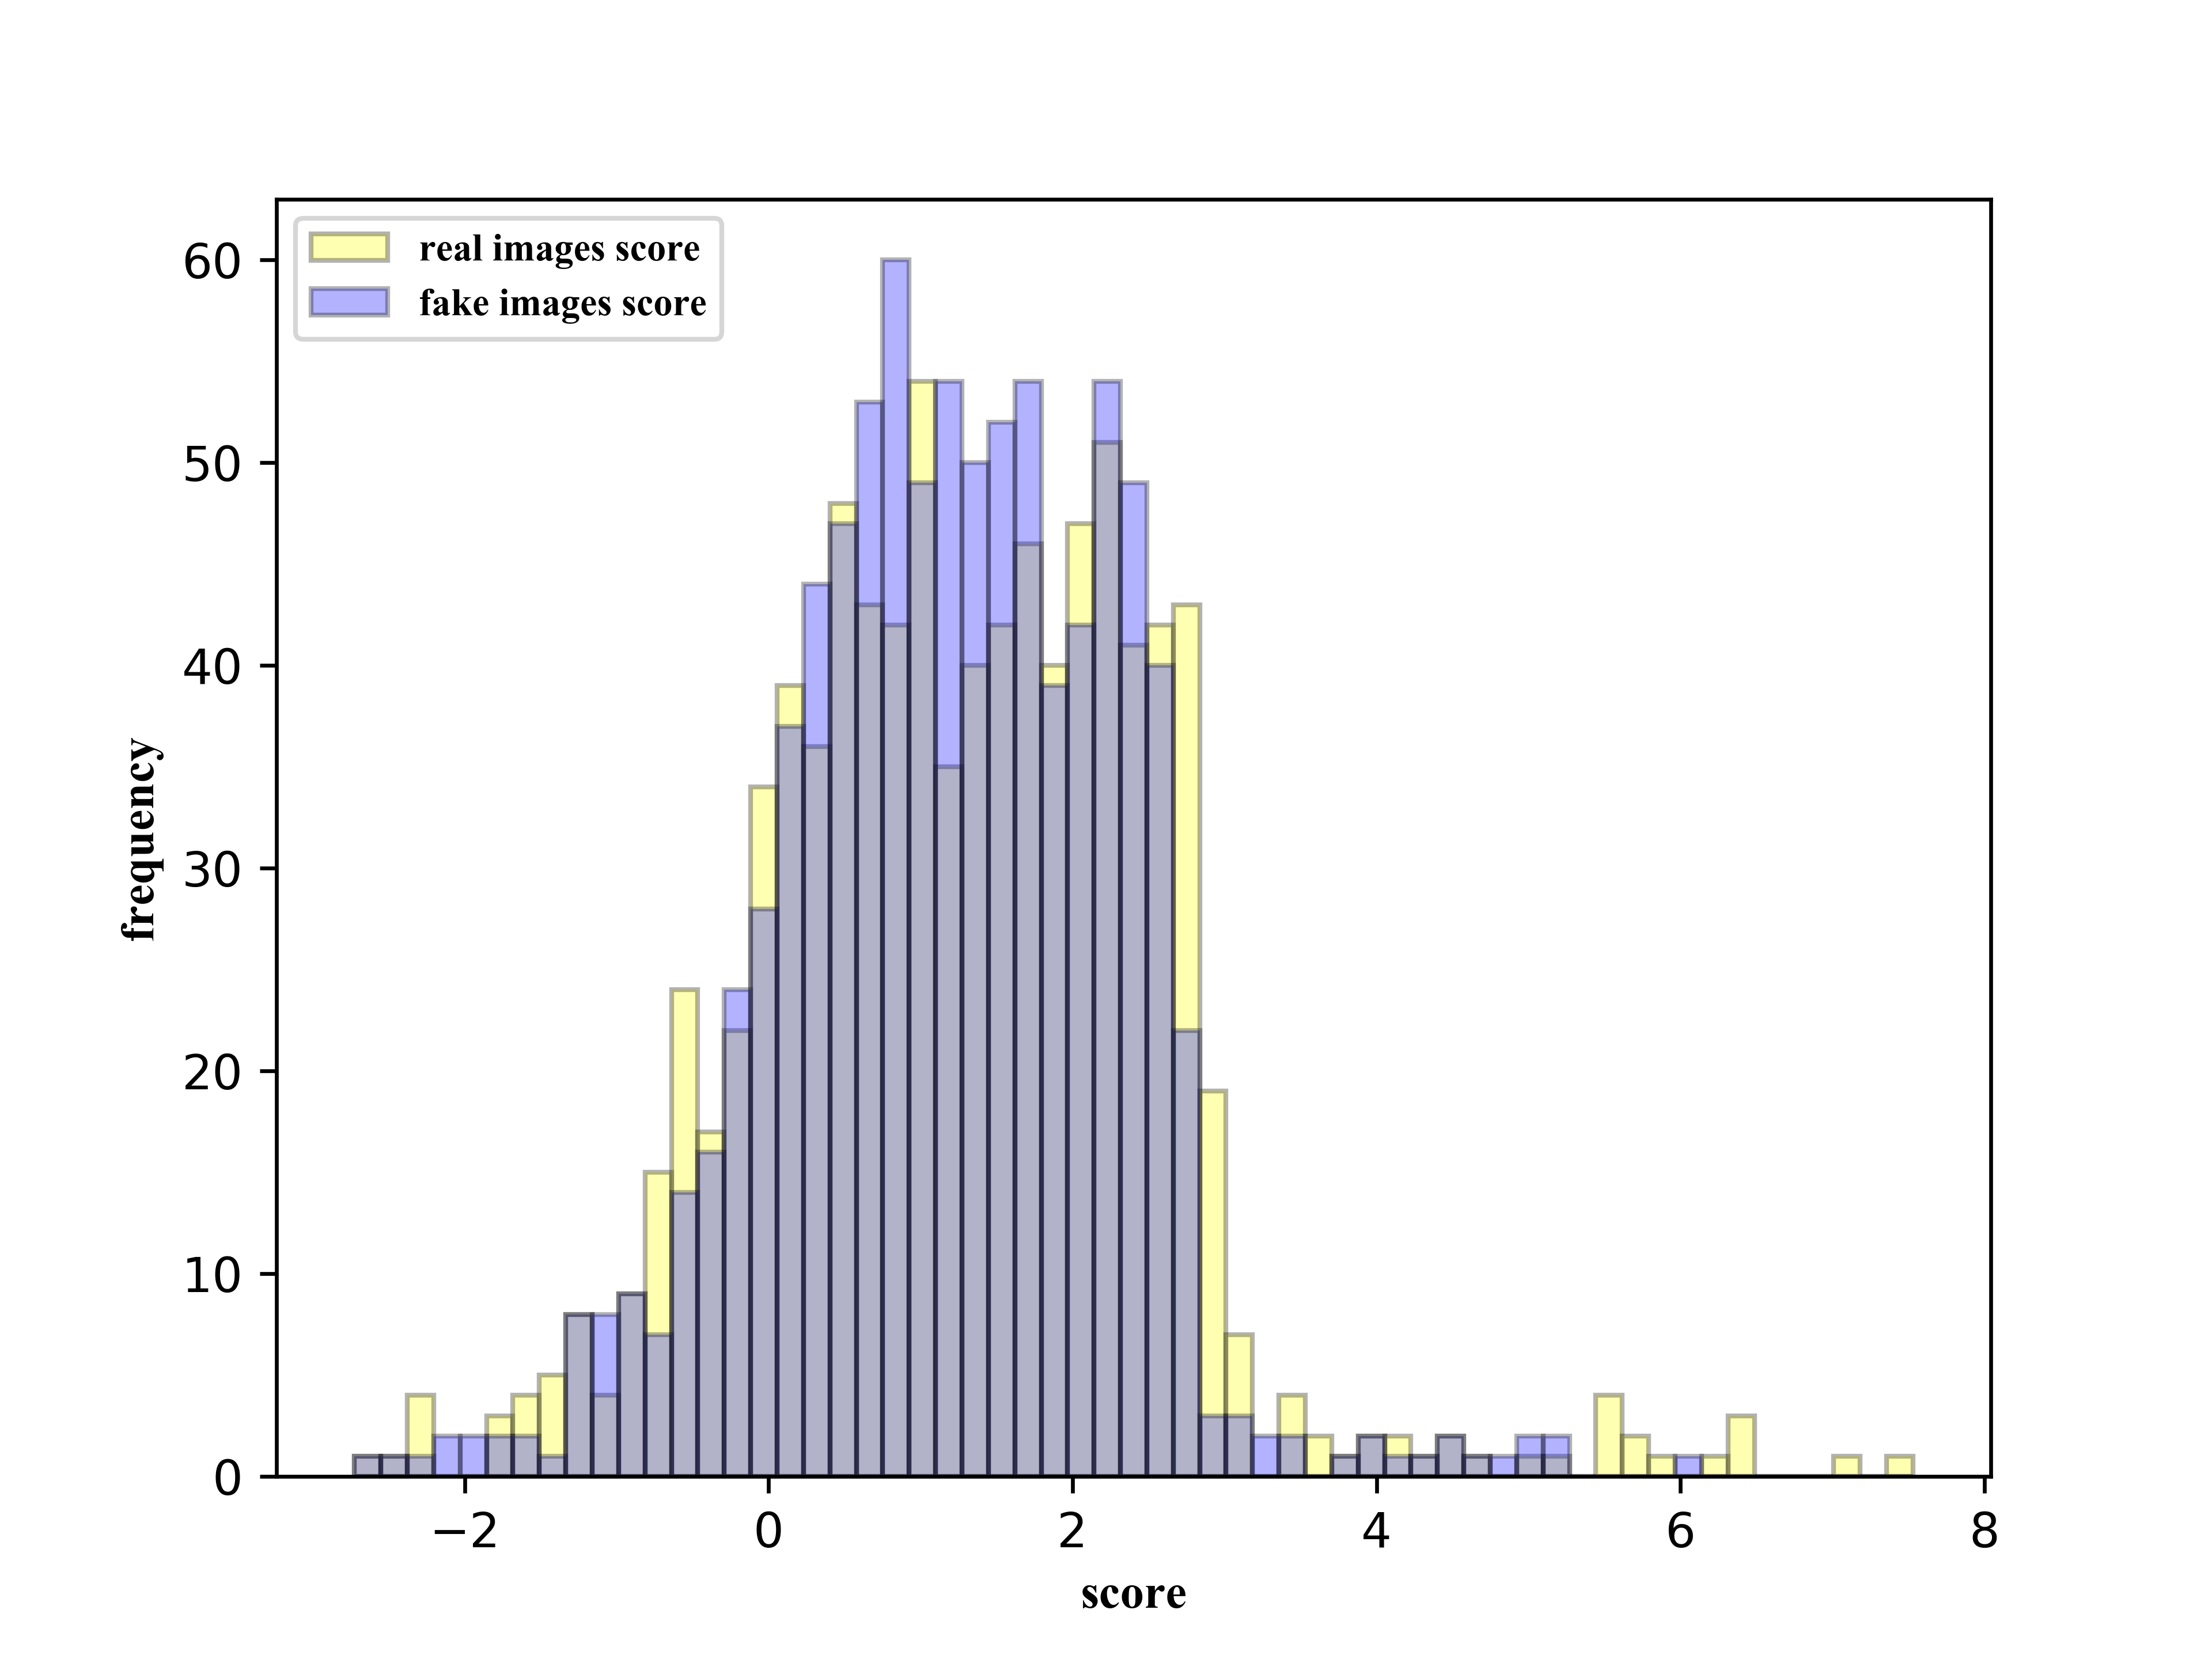
\includegraphics[width=1.0\textwidth]{figure/simulated_skin_score_distribution.png}
	\caption{将原始数据集中的正常图像和“正常”数据集中的“正常”图像分别送入到判别器之后,根据输出分数绘制的频率分布直方图。黄色柱子表示判别器真图像输入端的输出分数,紫色柱子表示判别器假图像输入端的输出分数,灰色柱子表示以上两者的重叠部分。}
	\label{fig:simulated_skin_hist_freq}
\end{figure}

以上实验从额外训练的ResNet分类器简介说明本文提出的模型在定位并去除生物标记物方面具有较强能力。在本小节中,我们还将“正常”四类数据集中的正常图像和异常图像均送入判别器,从而从判别器角度再次验证上述结论,判别器输出分数的频率分布直方图如图\ref{fig:simulated_skin_hist_freq}所示。从图\ref{fig:simulated_skin_hist_freq}中我们可以发现根据判别器两端输出分数所绘制的频率直方图中有较大重叠面积。另外,根据以上频率直方图,我们计算得到判别器两端输出分数的平均数分别为$1.3 $和$1.2$。而初试参数下,我们计算得到判别器两端输出的平均分数分别为$2.5$和$-0.5$,这说明在训练结束后,判别器输出两端输入图像的相似性得到了极大提升(平均分数差距:$3.0\rightarrow 0.1$),进一步说明判别器很难分辨输入图像的真/假,从而证明编码器-解码器的异常图像输出已经十分接近正常图像输出,由此我们可以推断出编码器-解码器已经很好的定位并去除了异常图像中的生物标记物。

\section{不同超参数下的实验结果分析}\label{sec:multi_classes_hyper_paras}
在本小节中,本文继续探究在不同不同超参数$\lambda_{1}$和$\lambda_{2}$组合下,本文提出的模型在生物标记物定位任务上的性能表现,以评估本文提出的模型的鲁棒性。在学习率、优化器、迭代次数、模型结构等设置均保持不变的情况下,除了默认超参数组合外($\lambda_{1}=4.0,\lambda_{2}=20.0$),我们还选取了另外$6$组不同超参数。在多类模拟皮肤病病变数据集上完成了相关实验后,分别根据第一类异常、第二类异常和第三类异常图像所绘制的P-R曲线分别如图\ref{fig:multi_simulate_pr_curve_image_net_hyper_paras}、图\ref{fig:multi_simulate_pr_curve_skin_hyper_paras}和图\ref{fig:multi_simulate_pr_curve_circle_hyper_paras}所示。另外,为了更为直观看出不同超参数组合下的模型性能,我们还将根据以上P-R曲线计算得到的AUC分数列在表\ref{tab:simulated_skin_diff_parameters}中。

\begin{table}[H]
	\centering
	\caption{不同超参数组合下,本文提出的模型根据多类模拟皮肤病病变数据集中的三类异常图像计算得到的AUC分数列表。}		
	\label{tab:simulated_skin_diff_parameters}
	\resizebox{1.0\textwidth}{!}{
		\begin{tabular}{c|c|c|c|c|c|c|c}
			\toprule[2pt]
			& $\lambda_{1}=4,\lambda_{2}=20$ & $\lambda_{1}=1, \lambda_{2}=20$& $\lambda_{1}=10, \lambda_{2}=20$&
			
			$\lambda_{1}=4,\lambda_{2}=10$ & $\lambda_{1}=4,\lambda_{2}=50$ &
			$\lambda_{1}=0,\lambda_{2}=20$ &
			$\lambda_{1}=4, \lambda_{2}=0$\\
			\midrule[2pt]
			第一类异常	& $\textbf{0.236}$ &	$0.135 $ & $0.207$ & $0.084$ & $0.194$& $0.149$ &	$0.176$ \\\hline
			
			第二类异常	& $\textbf{0.962}$ &	$0.884 $ & $0.946$ & $0.627$ & $0.910$& $0.847$ & $0.644$	 \\\hline
			
			第三类异常	& $0.805$ &	$0.750 $ & $\textbf{0.823}$ & $0.226$ & $0.779$& $0.714$ & $0.505$	 \\\hline
			
			Average AUC	& $\textbf{0.668}$ &	$0.590 $ & $0.659$ & $0.312$ & $0.628$& $0.570$ &	$0.442$ \\
			\bottomrule[2pt]
		\end{tabular}
	}
\end{table}


\begin{figure}[h]
	\centering
	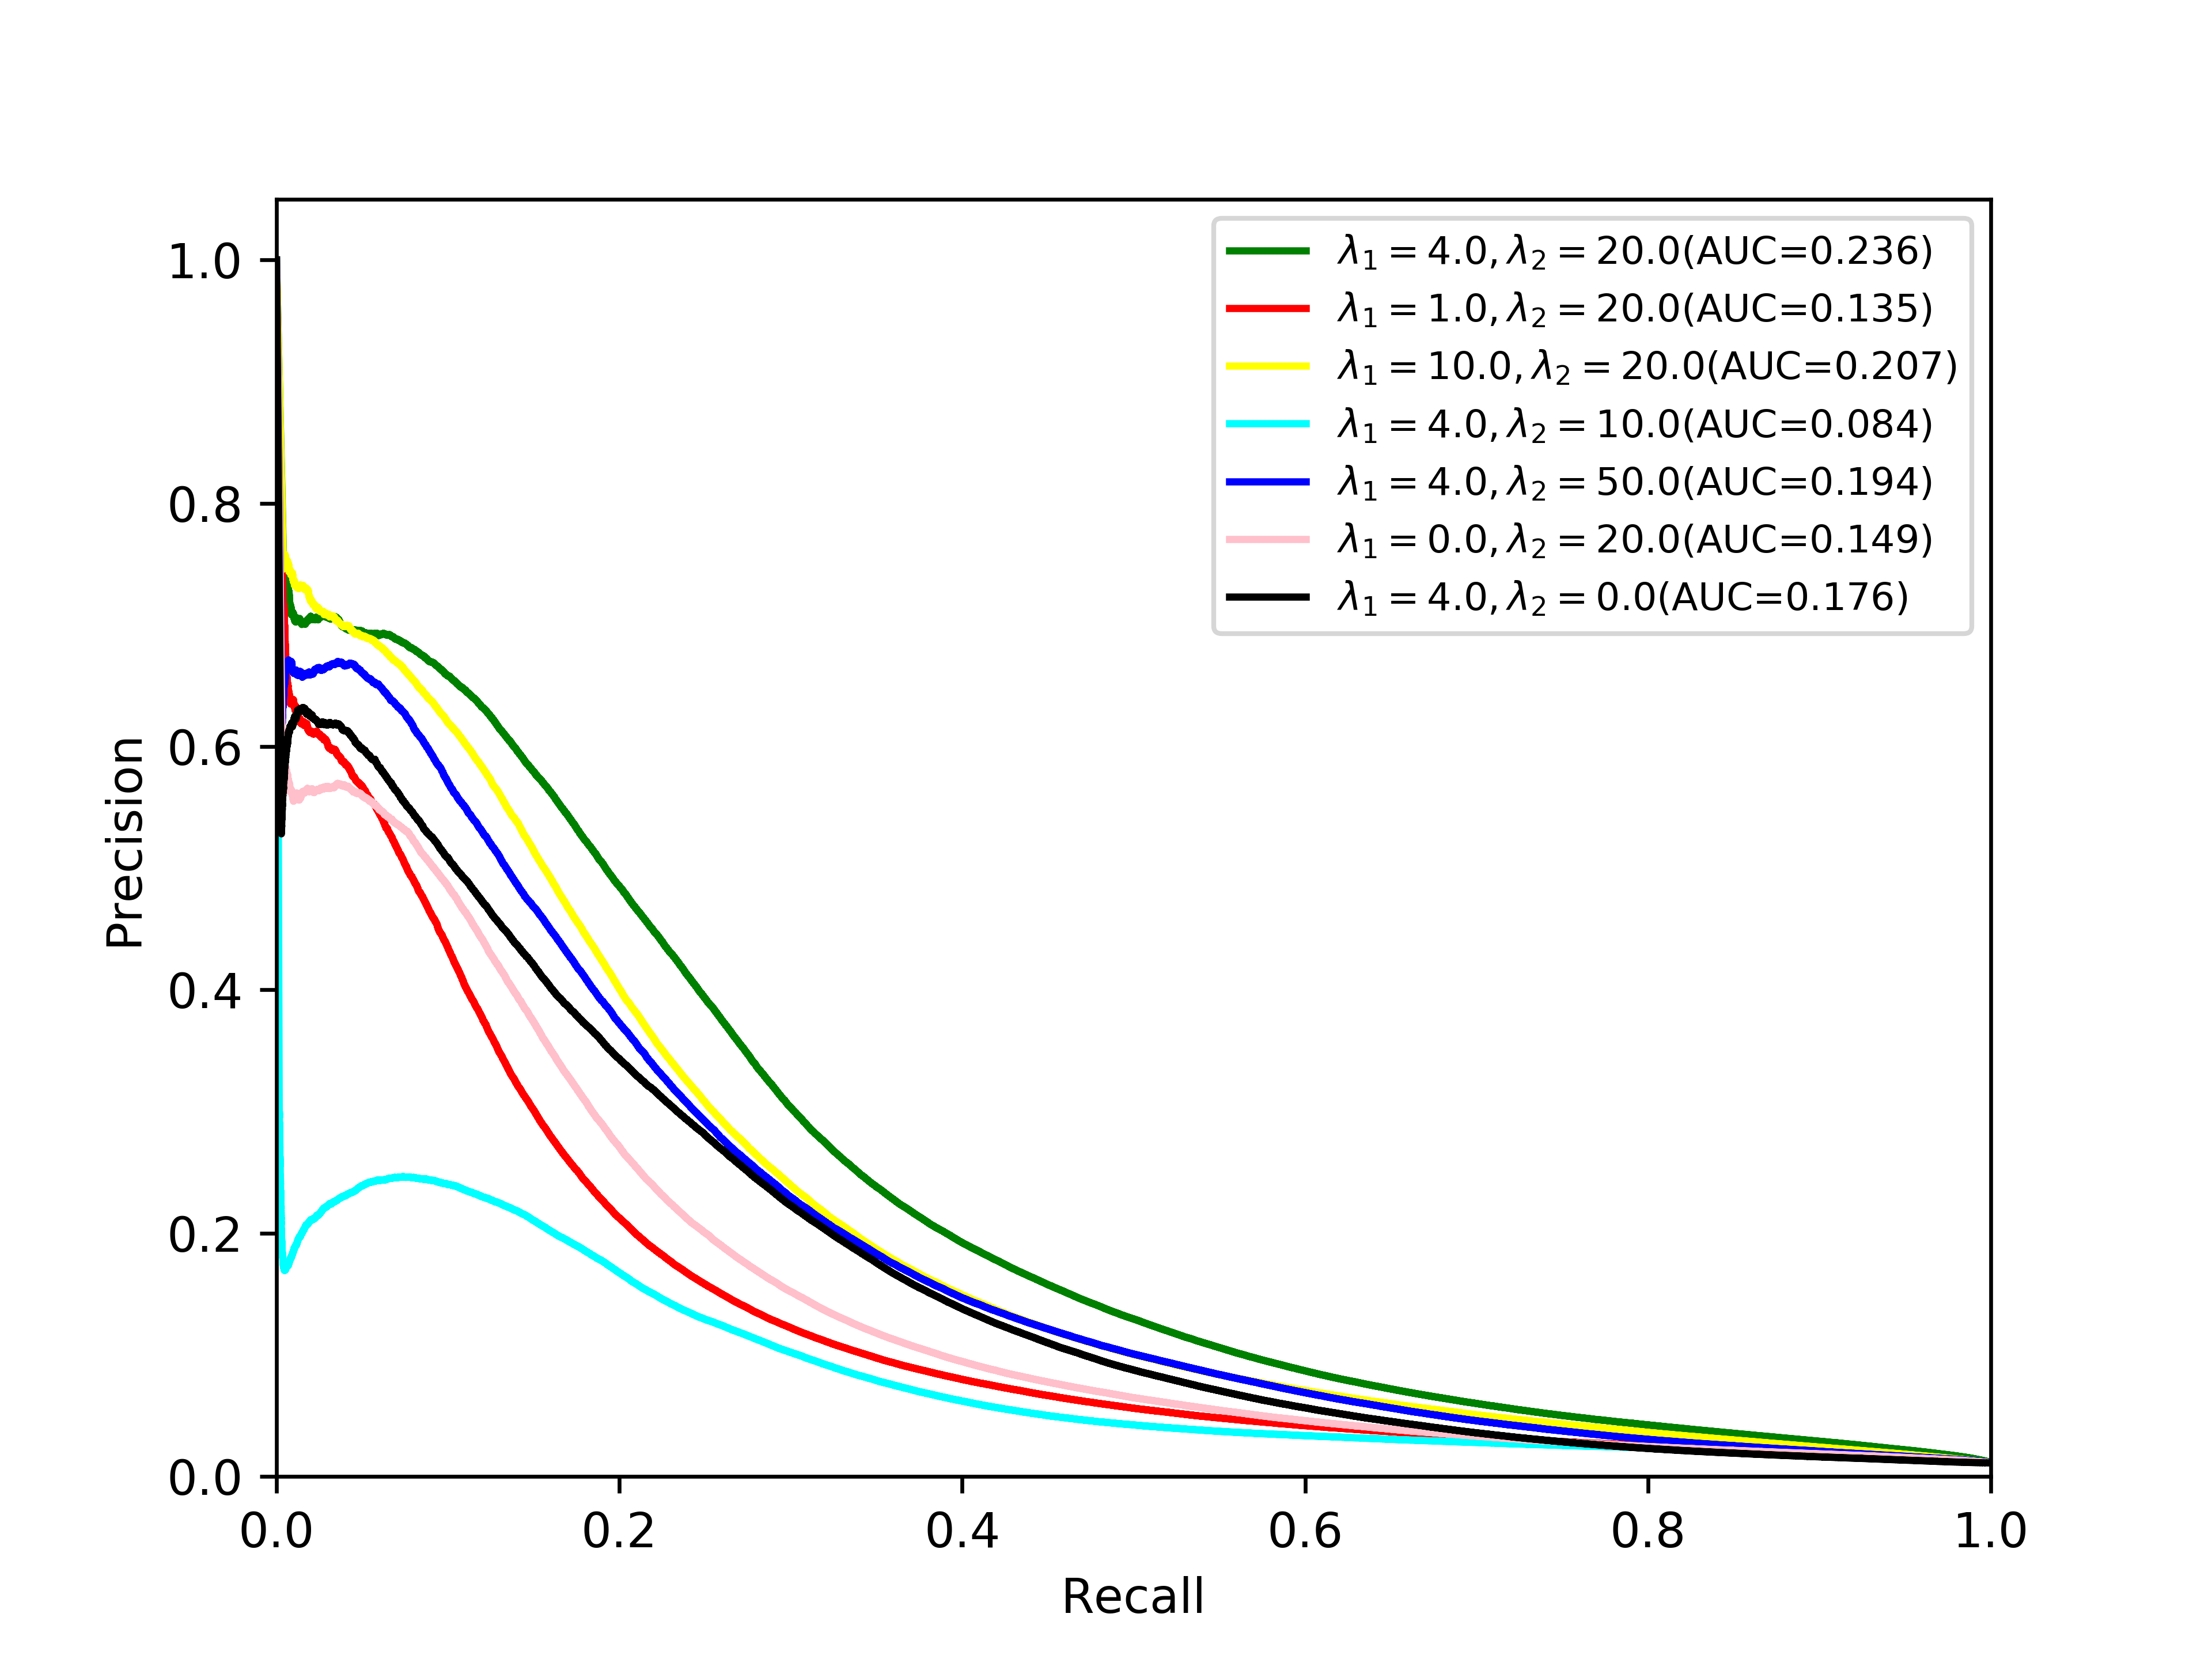
\includegraphics[width=1.0\textwidth]{figure/pr_curve_multi_skin_hyper_paras/IMAGE_NET_pr_curve.png}
	\caption{不同超参数组合下,本文提出的模型根据多类模拟皮肤病病变数据集中的第一类异常图像画出的P-R曲线及其各自曲线下的面积(AUC,见右上角图例)。} 
	\label{fig:multi_simulate_pr_curve_image_net_hyper_paras}
\end{figure}
\vspace{-0.2cm}
\begin{figure}[h]
	\centering
	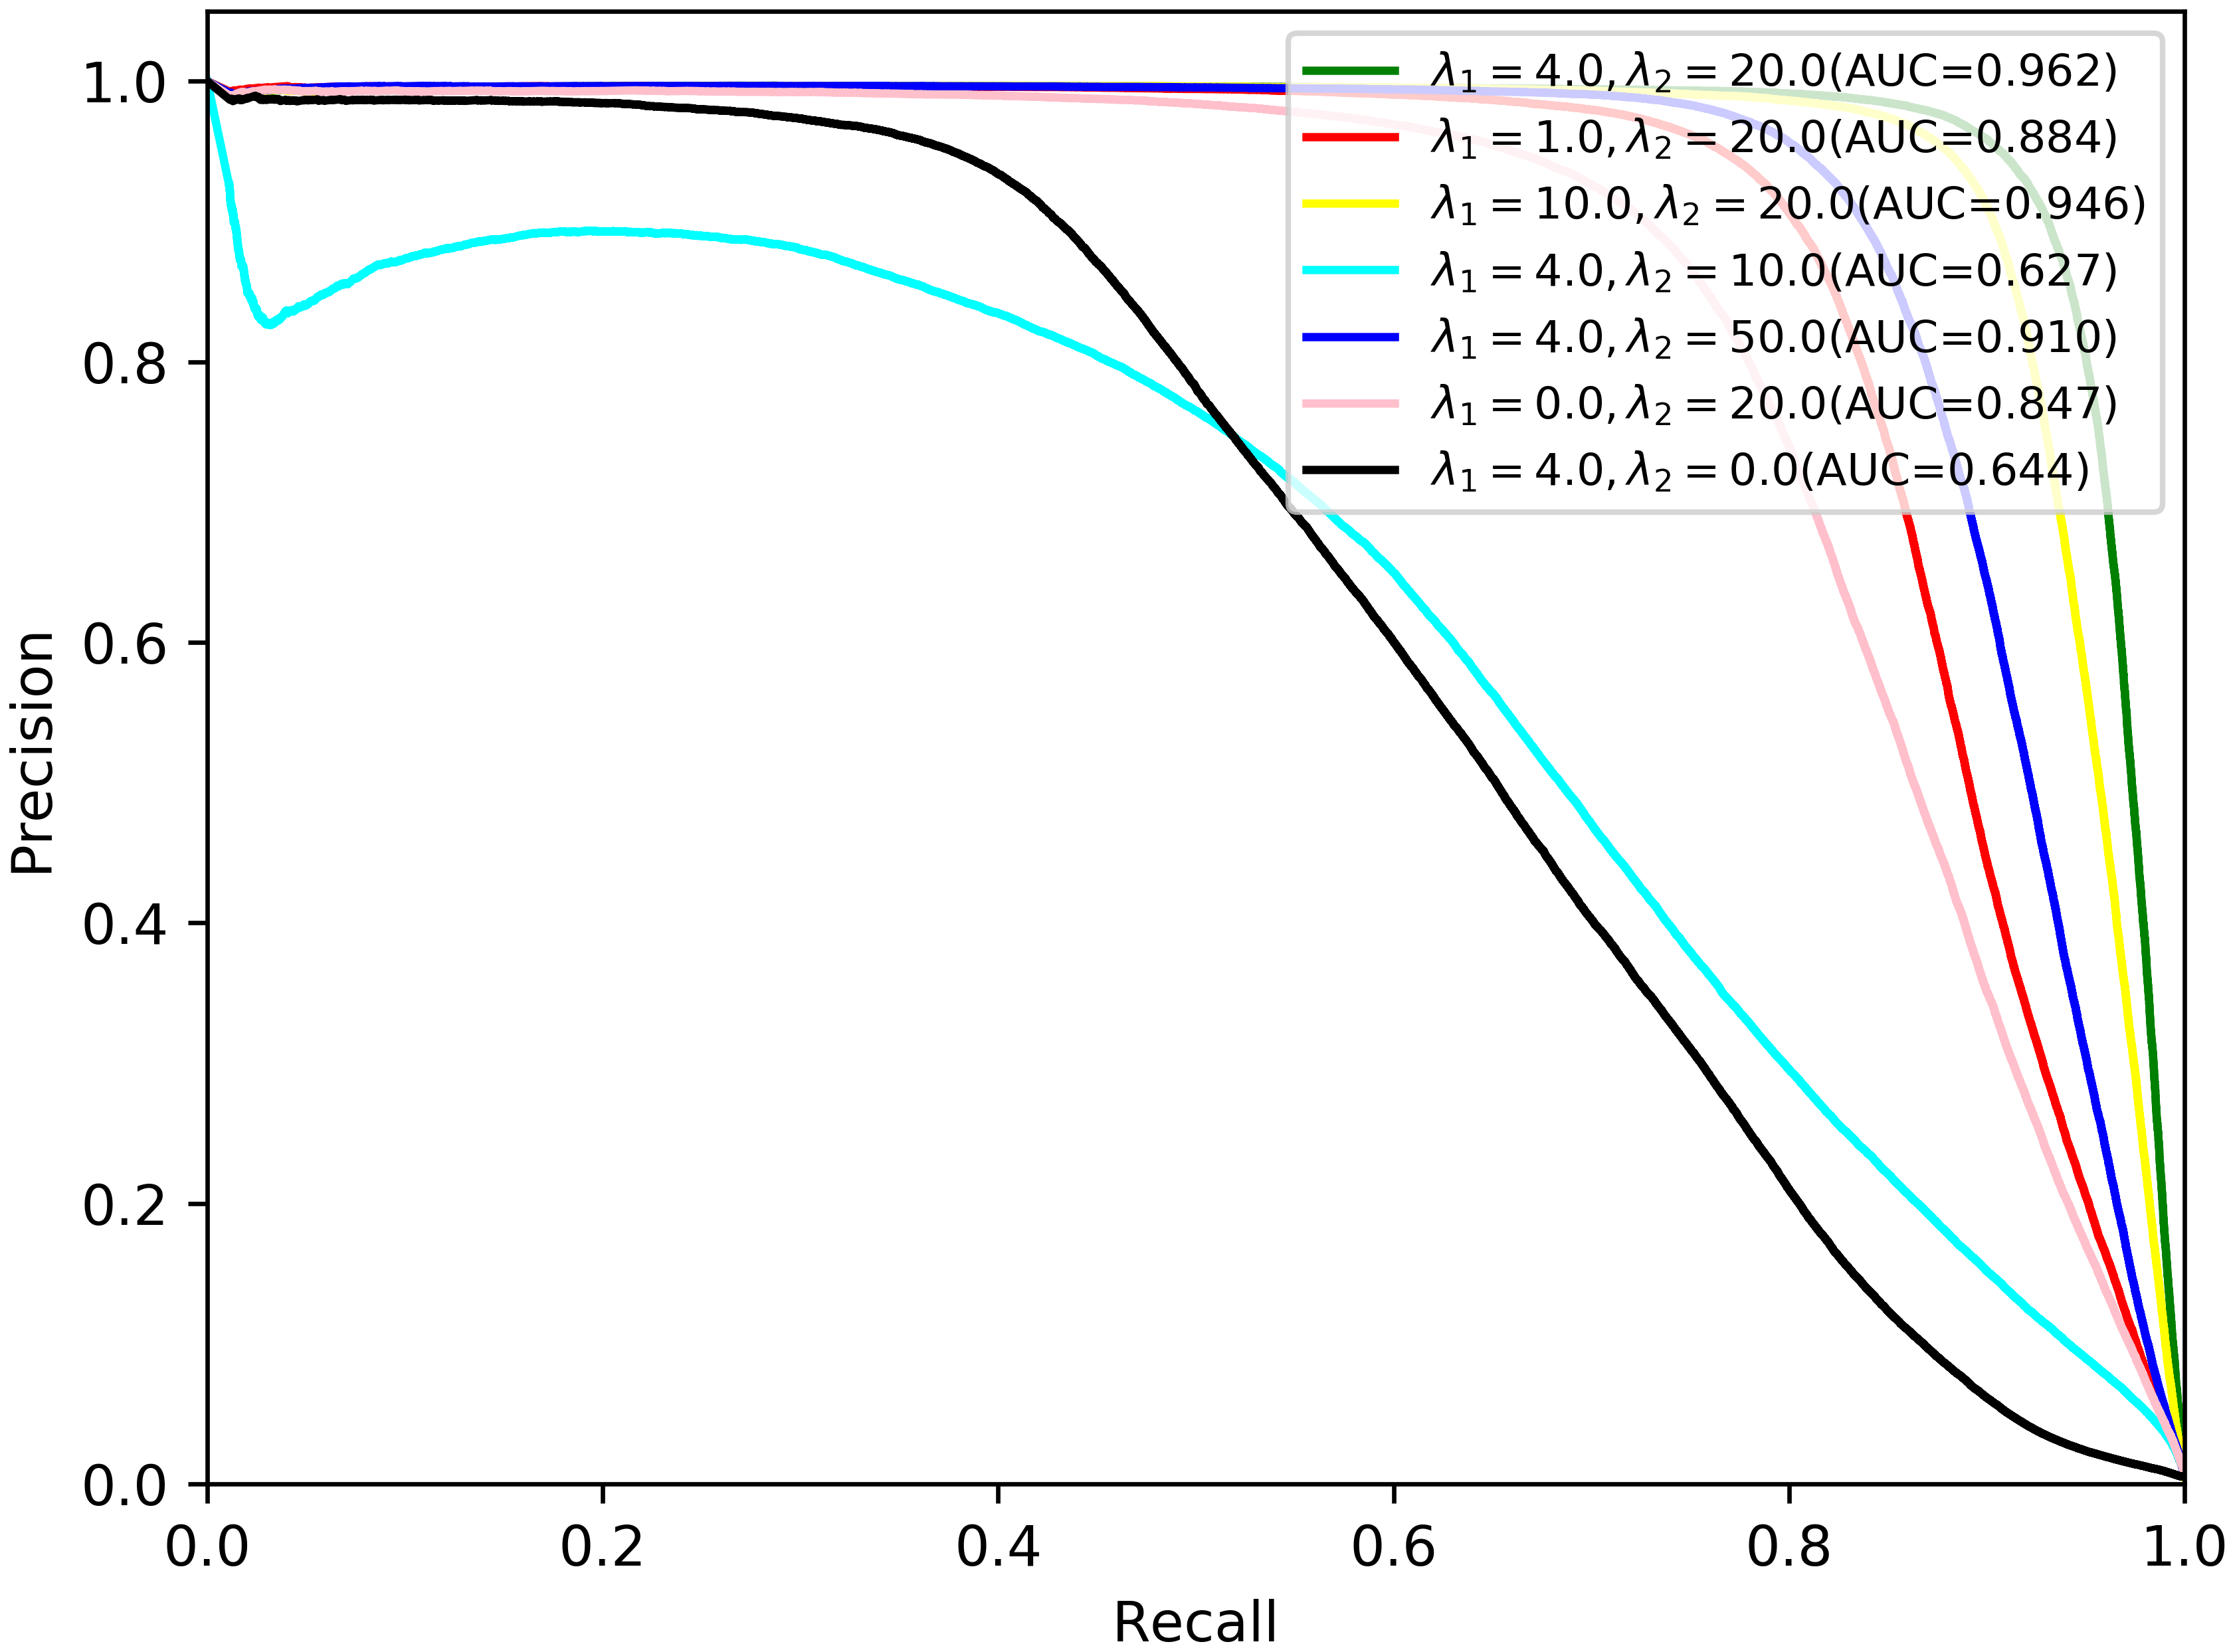
\includegraphics[width=1.0\textwidth]{figure/pr_curve_multi_skin_hyper_paras/SKIN_pr_curve.png}
	\caption{不同超参数组合下,本文提出的模型根据多类模拟皮肤病病变数据集中的第二类异常图像画出的P-R曲线及其各自曲线下的面积(AUC,见右上角图例)。}
	\label{fig:multi_simulate_pr_curve_skin_hyper_paras}
\end{figure}
\vspace{-0.8cm}
\begin{figure}[H]
	\centering
	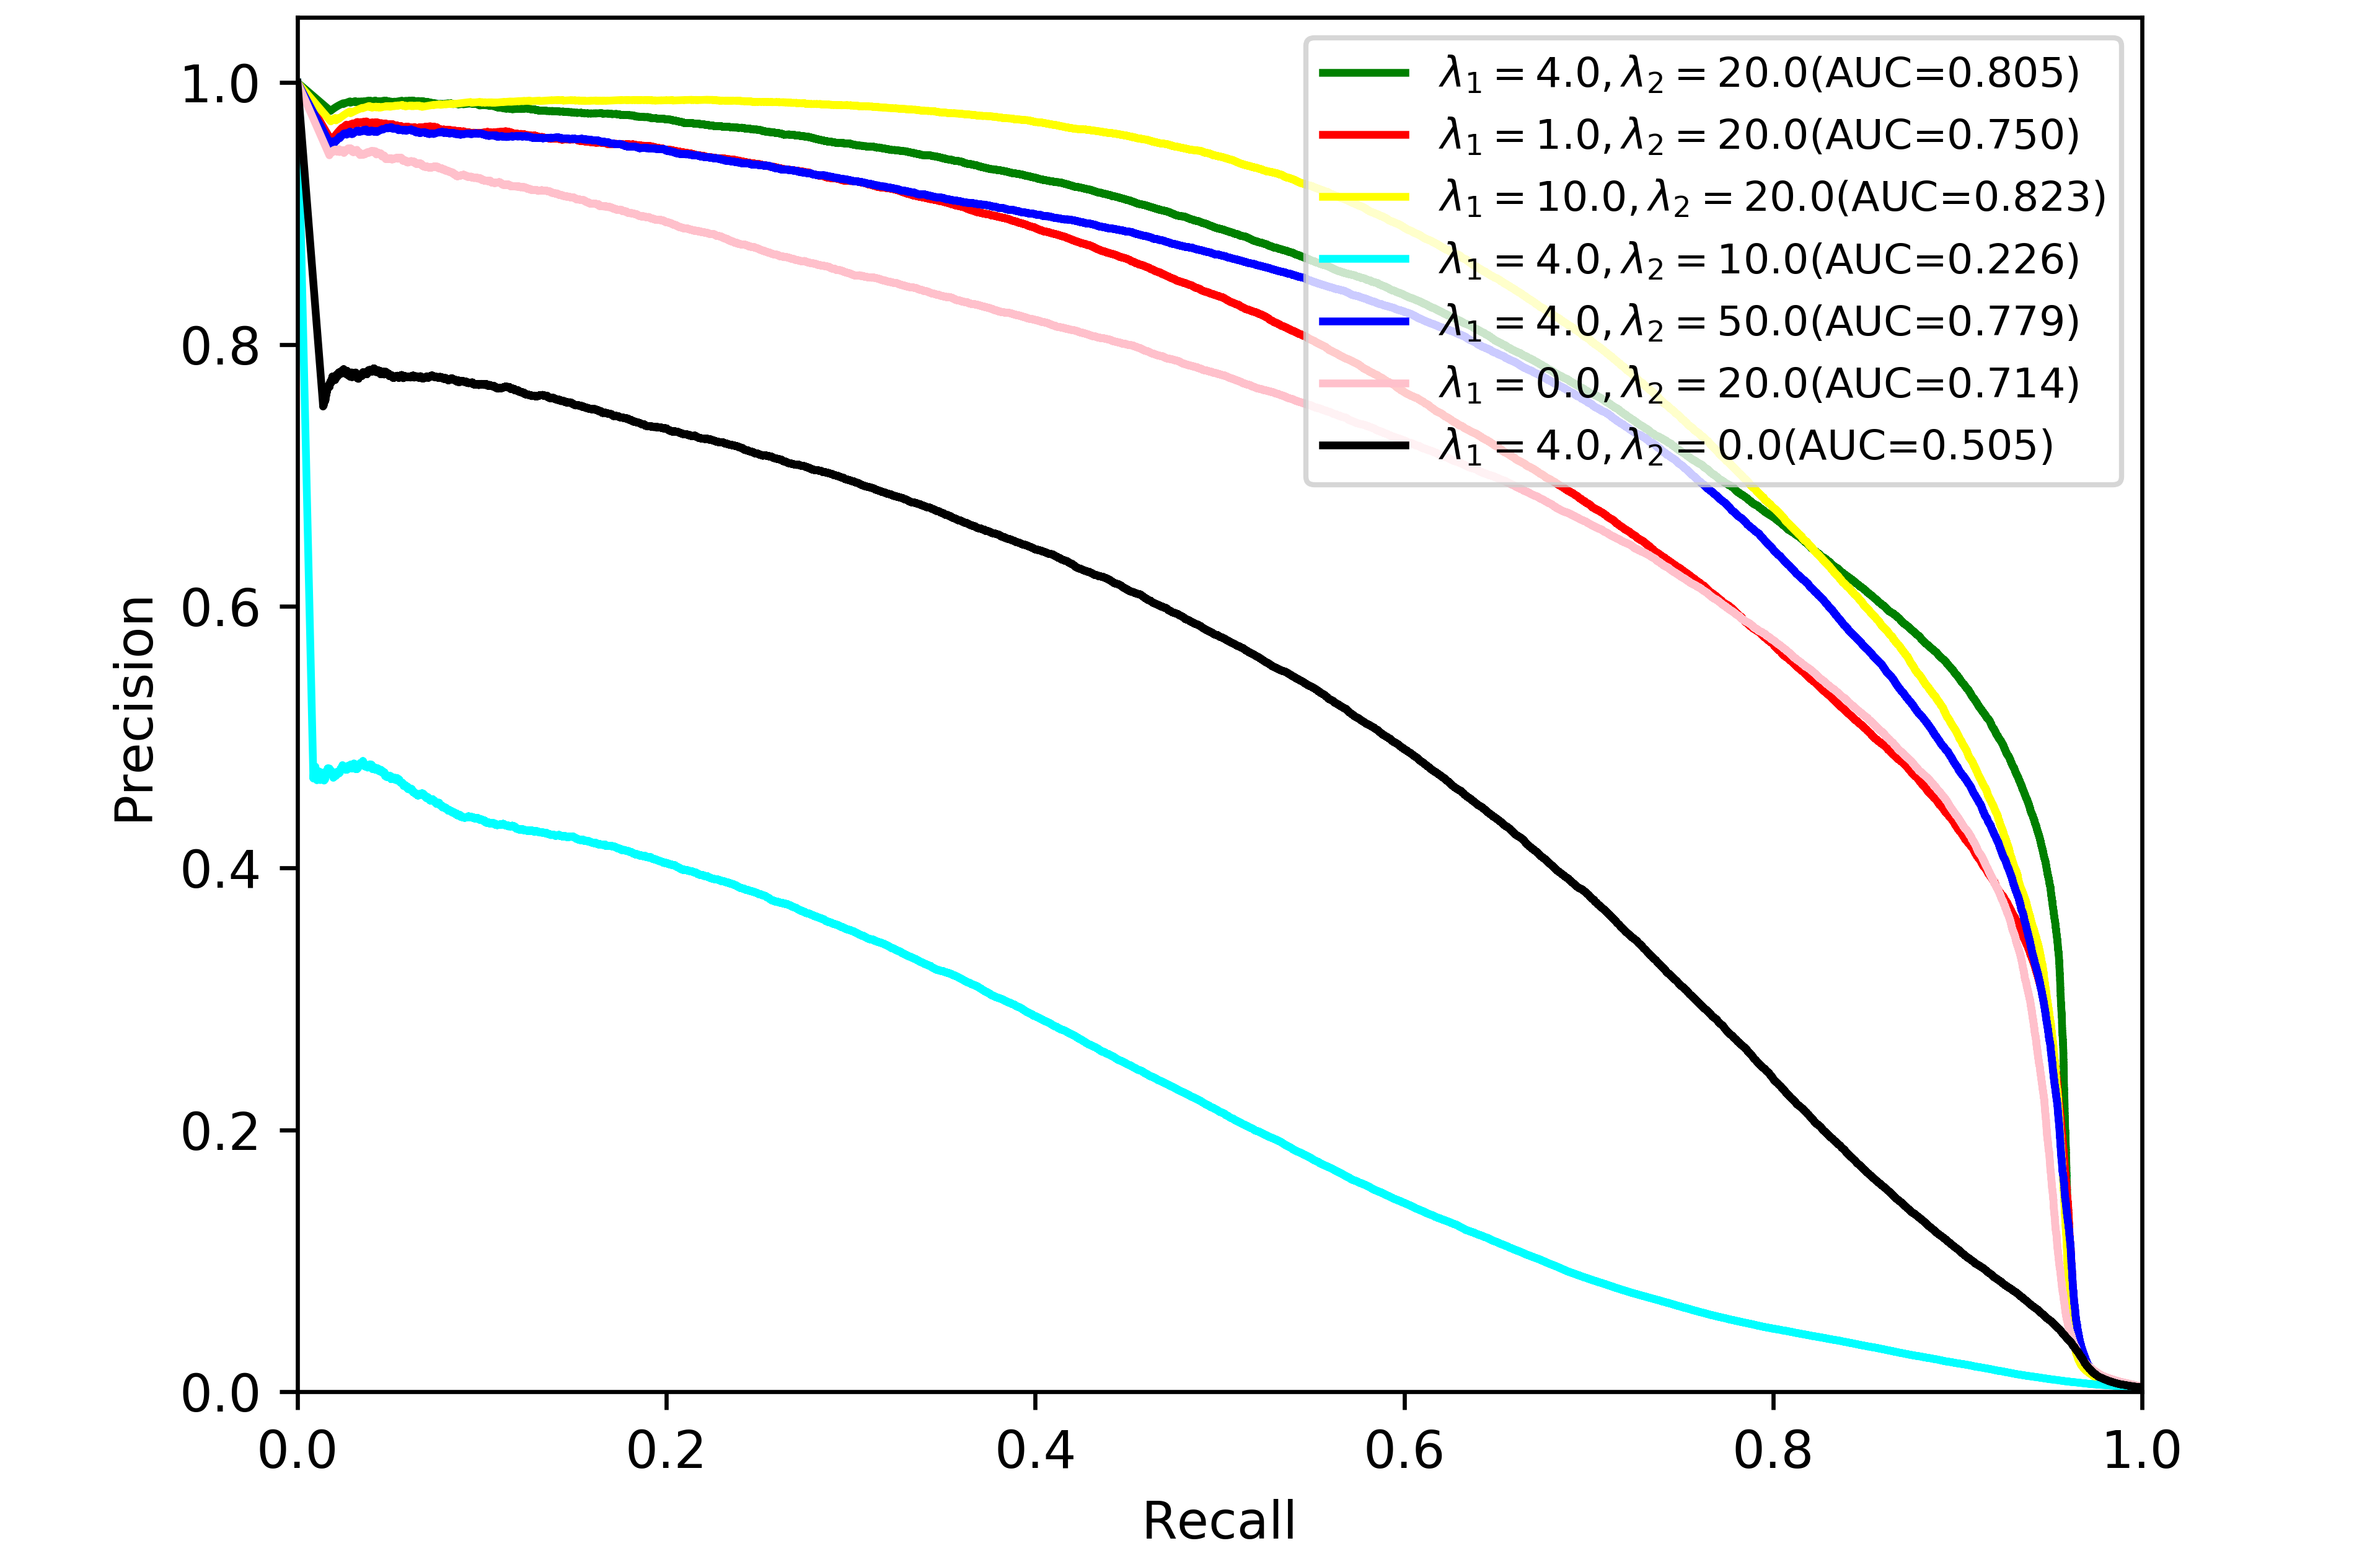
\includegraphics[width=1.0\textwidth]{figure/pr_curve_multi_skin_hyper_paras/CIRCLE_pr_curve.png}
	\caption{不同超参数组合下,本文提出的模型根据多类模拟皮肤病病变数据集中的第三类异常图像画出的P-R曲线及其各自曲线下的面积(AUC,见右上角图例)。} 
	\label{fig:multi_simulate_pr_curve_circle_hyper_paras}
\end{figure}


从表\ref{tab:simulated_skin_diff_parameters}的平均AUC分数可以看出,本文的默认$\lambda_{1}$和$\lambda_{2}$超参数组合对生物标记物的定位性能最佳。从各类异常上个AUC分数来看,除了第二类异常外,本文的默认参数均取得了最高AUC分数。我们还能发现,当超参数$\lambda_{1}$偏小时,比如$\lambda_{1}=1$(表中第$3$列),本文提出的模型(以下简称“模型”)取得的平均AUC较低($0.590$),与默认超参数相比有所下降,极端情况下($\lambda_{1}=0$)更是如此(表中第$7$列,平均AUC=$0.570$)。这是因为CNN分类器在模型中主要负责定位生物标记物(实验验证参见\ref{sec:g_c_g_d_g_d_c_comparsion}小节),一旦CNN分类器在模型中占的权重($\lambda_{1}$)较小,这显然会导致模型定位生物标记物的定位精确度有所下降。当超参数$\lambda_{2}$偏小时,比如$\lambda_{2}=10$和$\lambda_2=0$,此时L1损失函数所占权重较小,则模型对图像修改的约束将会降低,那么模型在修改生物标记物所在的像素强度的同时显然会不可避免地修改正常区域的像素强度,因此模型取得的平均AUC更低,平均AUC分别为$0.312$(表中第$5$列)和$0.442$(表中第8列)。反之,当$\lambda_{1}(\ge 4)$和$\lambda_{2}(\le 20)$取值较大时,模型对生物标记物的定位性能较为稳定,如表中第$2$列($\lambda_{1}=4, \lambda_{2}=20$)、第$4$列($\lambda_{1}=10, \lambda_{2}=20$)和$6$列($\lambda_{1}=4, \lambda_{2}=50$)中模型取得平均AUC分别为$0.668$、$0.659$、$0.628$,可证明模型的超参数适用范围较广,具有较好的鲁棒性。根据三类异常图像所绘制的P-R曲线(参见图\ref{fig:multi_simulate_pr_curve_image_net_hyper_paras}、图\ref{fig:multi_simulate_pr_curve_skin_hyper_paras}和图\ref{fig:multi_simulate_pr_curve_circle_hyper_paras})同样可证明以上结论。

\section{本章小结}
本章主要将本文提出的方法由二类问题推广到多类问题,在此过程中,本文对原始二类模型进行了相关改进,比如,将二类交叉熵损失函数替换成多类交叉熵损失函数、将所有异常类看成判别器的假图像输入端等,以最小的代价实现二类问题到多类问题的扩展,并在多类模拟皮肤病病变数据集上进行了相关实验评估,与CAM和Grad-CAM相比,分别从定性分析(热图)和定量分析(P-R曲线及其AUC)两个角度直接说明本文提出的模型能够更准确地定位到生物标记物的位置,具有更加优异的性能。除此之外,本文还分别从额外训练的CNN分类器的角度和判别器的角度再次证明了上述结论。最后,为了说明本文提出的方法的超参数鲁棒性,本文还对不同超参数$\lambda_{1}$和$\lambda_{2}$组合进行了测试。到此,本文所有实验内容叙述完毕。在接下来一章中,我们将对本文工作进行总结,并对将来的研究方向进行展望。


        %\newclearpage
        \chapter{总结与展望}
%本章是毕业论文的总结,是整篇论文的归宿,应精炼、准确、完整。应着重阐述自己的创造性成果及其在本研究领域中的意义、作用,还可进一步提出需要讨论的问题和建议。
%卷积神经网络可视化
\section{工作总结}
%近些年来,随着计算机技术的蓬勃发展及其在医学影像领域的广泛应用,疾病标记物定位方法也不断取得进步。由于医学图像的标注代价高昂、难以大量获得,故在弱监督条件(提供图像级标签,需要给出像素级定位结果)下实现疾病标记物的定位就具有较大的研究价值和实际意义。针对弱监督条件下的疾病标记物定位问题,目前主要有包括多示例学习和卷积神经网络可视化在内的两种计算机方法可解决疾病标记物定位这一问题。但是在面对分布广泛、尺寸大小不一的疾病标记物时,以上方法均只能定位到疾病标记物的大概位置,同时还会伴随着将正常区域也误认为疾病标记物和遗漏疾病标记物的的情况发生,无法在弱监督条件下实现疾病标记物的精确定位。为了克服以上方法的缺陷,在弱监督条件下实现疾病标记物的精确定位,本文从图像生成的角度,创造性地组合了CNN分类器和判别器,提出了一种新型网络结构。随后在三个数据集上均进行了相关性能的测试,分别处理了二类问题和多类问题,并与当前流行的卷积神经网络可视化方法做了详尽的比较。从定性分析(热图)和定量分析(P-R曲线及其AUC)两个角度来看,本文提出的方法均取得了目前最佳的性能表现,在保证定位疾病标记物的精确性的同时还能兼顾其全面性(不会遗漏难以察觉的微小疾病标记物)。本文的工作总结如下:

在弱监督条件(提供图像级标签,需要给出像素级结果)下,面对分布广泛、尺寸大小不一的疾病标记物定位任务,本文从图像生成的角度,创造性地组合了CNN分类器和判别器,提出了一种新型网络结构。随后在三个数据集上均进行了相关性能的测试,分别处理了二类问题和多类问题,并与当前流行的卷积神经网络可视化方法做了详尽的比较。从定性分析(热图)和定量分析(P-R曲线及其AUC)两个角度来看,本文提出的方法均取得了目前最佳的性能表现,在保证定位疾病标记物的精确性的同时还能兼顾其全面性(不会遗漏难以察觉的微小疾病标记物)。本文的工作总结如下:

1)本文极具创造性地组合了CNN分类器和生成生成网络,提出了一种较为新颖的网络模型,CNN分类器负责定位生物疾病标记物并尽量去除疾病标记物,生成对抗网络负责进一步完全去除疾病标记物,并采用CNN分类器和生成对抗网络交替训练的方式来实现以上设想。面对在图像中分布广泛、尺寸大小不一的疾病标记物,无论是多示例学习还是卷积神经网络可视化方法,都只能大概定位到疾病标记物的位置,往往还会忽略图像中难以察觉的疾病标记物,这主要是多示例学习中需要对图像的分块取样操作和卷积神经网络可视化方法中对特征图的上采样操作造成的。为了克服以上问题,本文从图像生成的角度出发,避免对图像的分块操作和上采样操作,通过生成图像减去输入图像来给出疾病标记物的准确位置。另外,由于图像中的疾病标记物所占比例极小,故使用L1损失函数来加以约束,从而尽量保证正常像素的像素强度保持不变。

2)我们首先将本文提出的方法用于处理二类疾病标记物定位问题,相比于神经网络可视化方法,无论是从定性分析还是从定量分析的角度,本文提出的方法的表现更为出色。与此同时,我们还将本文提出的方法用于处理多类疾病标记物定位问题,在此过程中,由于天然的数据不均衡现象存在和生成对抗网络自身的限制,我们对数据加载和损失函数均做出了相关改进。首先,我们将二类交叉熵换成了多类交叉熵损失函数并将CNN分类器输出端扩展到了多个。另外,我们还将所有异常类看做生成对抗网络的假图像输入,这样既避免了额外的网络引入,又能最大限度减少额外的计算资源开销。通过以上系列微调,我们成功将本文提出的方法应用到了多类疾病标记物定位任务中,与卷积神经网络可视化方法相比,文本提出的方法同样取得了目前最佳的性能表现,从而证明了本文提出的方法的应用广泛性和鲁棒性。

%在只提供图像级标注,要求给出像素级定位结果的弱监督条件下,目前是没有深度学习方法能直接较好地精确定位疾病标记物。因此,本文提出的新颖深度学习模型填补了这个问题的空白。
定位疾病标记物不仅为发现更多潜在疾病标记物提供了技术基础,还能辅助专业医师诊断疾病,这有利于缓解专业医师繁重的工作。同时,由于本文提出的方法只需要提供图像级标注,这能够大大降低图像的标注成本。

\section{研究展望}
虽然本文提出的方法能,无论是在二类疾病标记物定位任务还是在多类疾病标记物定位任务上,都能取得比较好的性能。但是本文提出的方法还存在以下不足:

% gan训练
1)众所周知,训练生成对抗网络的训练过程存在震荡现象,而由编码器-解码器与判别器组成的生成对抗网络是本文提出的模型的重要组成部分,虽然WGAN-GP(本文采用的生成对抗网络)在理论上证明添加梯度惩罚可以避免梯度消失与梯度爆炸,但是当实验参数设置不当时,仍然会发生梯度更新过猛的现象,具体表现在随着训练过程的进行,判别器输出分数的绝对值不断增大,最终导致训练失败。

% 图片size大小
2)本文所有实验的输入图像尺寸大小均为$128\times 128$,这主要是考虑到由于眼底图像含有大量丰富的细节,图片尺寸过大不仅会增加编码器-解码器的模型复杂度(主要是网络深度),还会增加编码器-解码器重建图片的难度。但是实际上原始眼底图像的尺寸大小大于$1000\times 1000$,就会导致原始图像中的部分细节纹理信息的丢失。

本文提出的方法除了存在以上不足外,本文提出的方法在处理疾病的多样性方面还能从以下思路进行下一步扩展与延伸:

1)无论是二类糖尿病病变数据集,还是二类/多类模拟皮肤数据集,其中疾病标记物的共同特点是分布广泛、尺寸大小不一。除此之外,异常区域的像素总量在整张图像中只占了极少一部分($\le 5\%$),这也是在本文损失函数中加入L1约束的主要原因。所以本文接下来的研究内容可以针对异常区域占比较大的疾病,比如黑色素瘤病变。对于此类异常区域占比比较大的图像,L1约束显然不再适用。因此还需要对损失函数进行相关改进,其中比较好的方案是根据图像中被修改的像素数量也设置惩罚,一旦被修改的像素数量超过某个阈值,则施加惩罚。否则,损失惩罚为$0$。

2)在本文使用到的数据集中,无论是二类数据集还是多类数据集,总体而言,各个类别之间只是存在轻微数据不均衡,各个类别之间的图像数量之比比较接近$1:1$。而在临床情况下,很多疾病是非常少见的,比如斑色鱼鳞癣、大疱性表皮松解症等极其罕见的皮肤病。如果能在图像中准确定位到这类罕见疾病的疾病标记物,这将有重要实际意义和临床意义。不过这种情况下在图像中定位到疾病标记物,除了要面对样本不均衡问题外,很有可能还需要解决小样本问题。

3)本文提出的方法处理的图像均是与皮肤图像镜或者眼底图像相关,这些图像中的疾病标记物与背景相比均是存在颜色、亮度、纹理等直观视觉特征上的区别。与以上图像不同的是,CT图像中的疾病标记物相对没有那么明显,区分度较小,比如在影像学上,CT肺部影像中实性结节和混合性结节比较容易发生混淆。因此,相比较而言CT影像中的病灶区域更加难以检测更不用说定位。但是,医院每天将会产生大量CT等影像,如果能将在这种影像中完成对疾病疾病标记物的定位,那么将会大大减轻专业医师的工作负担,产生较大的实际应用价值。

%总而言之,本文提出的模型的诸多地方都有待挖掘和改进。同时,本文的研究内容也有很多方向可以进行下一步扩展。

        %\newclearpage
        % 结语

    % 附录部分
    \backmatter
        % 参考文献
        \makereferences
        % MICCAI2019
        %\bibliographystyle{Bibliography/bibtex-style/MICCAI2019}
        % CVPR2019
        \bibliographystyle{Bibliography/bibtex-style/CVPR2019}
        \bibliography{Bibliography/Reference}
        %\newclearpage
        % 附录
    \appendix
        \chapter{ROC曲线补充说明}\label{chapter:append1}
如图\ref{fig:roc_cam_grad_cam_our_diabetic_retinopathy}所示,CAM、Grad-CAM和本文提出的模型根据二类视网膜糖尿病病变数据集绘制的ROC曲线。根据P-R曲线及其AUC,与CAM、Grad-CAM相比,本文提出的模型性能表现最佳(AUC最高为$0.922$)。
\begin{figure}[H]
	\centering
	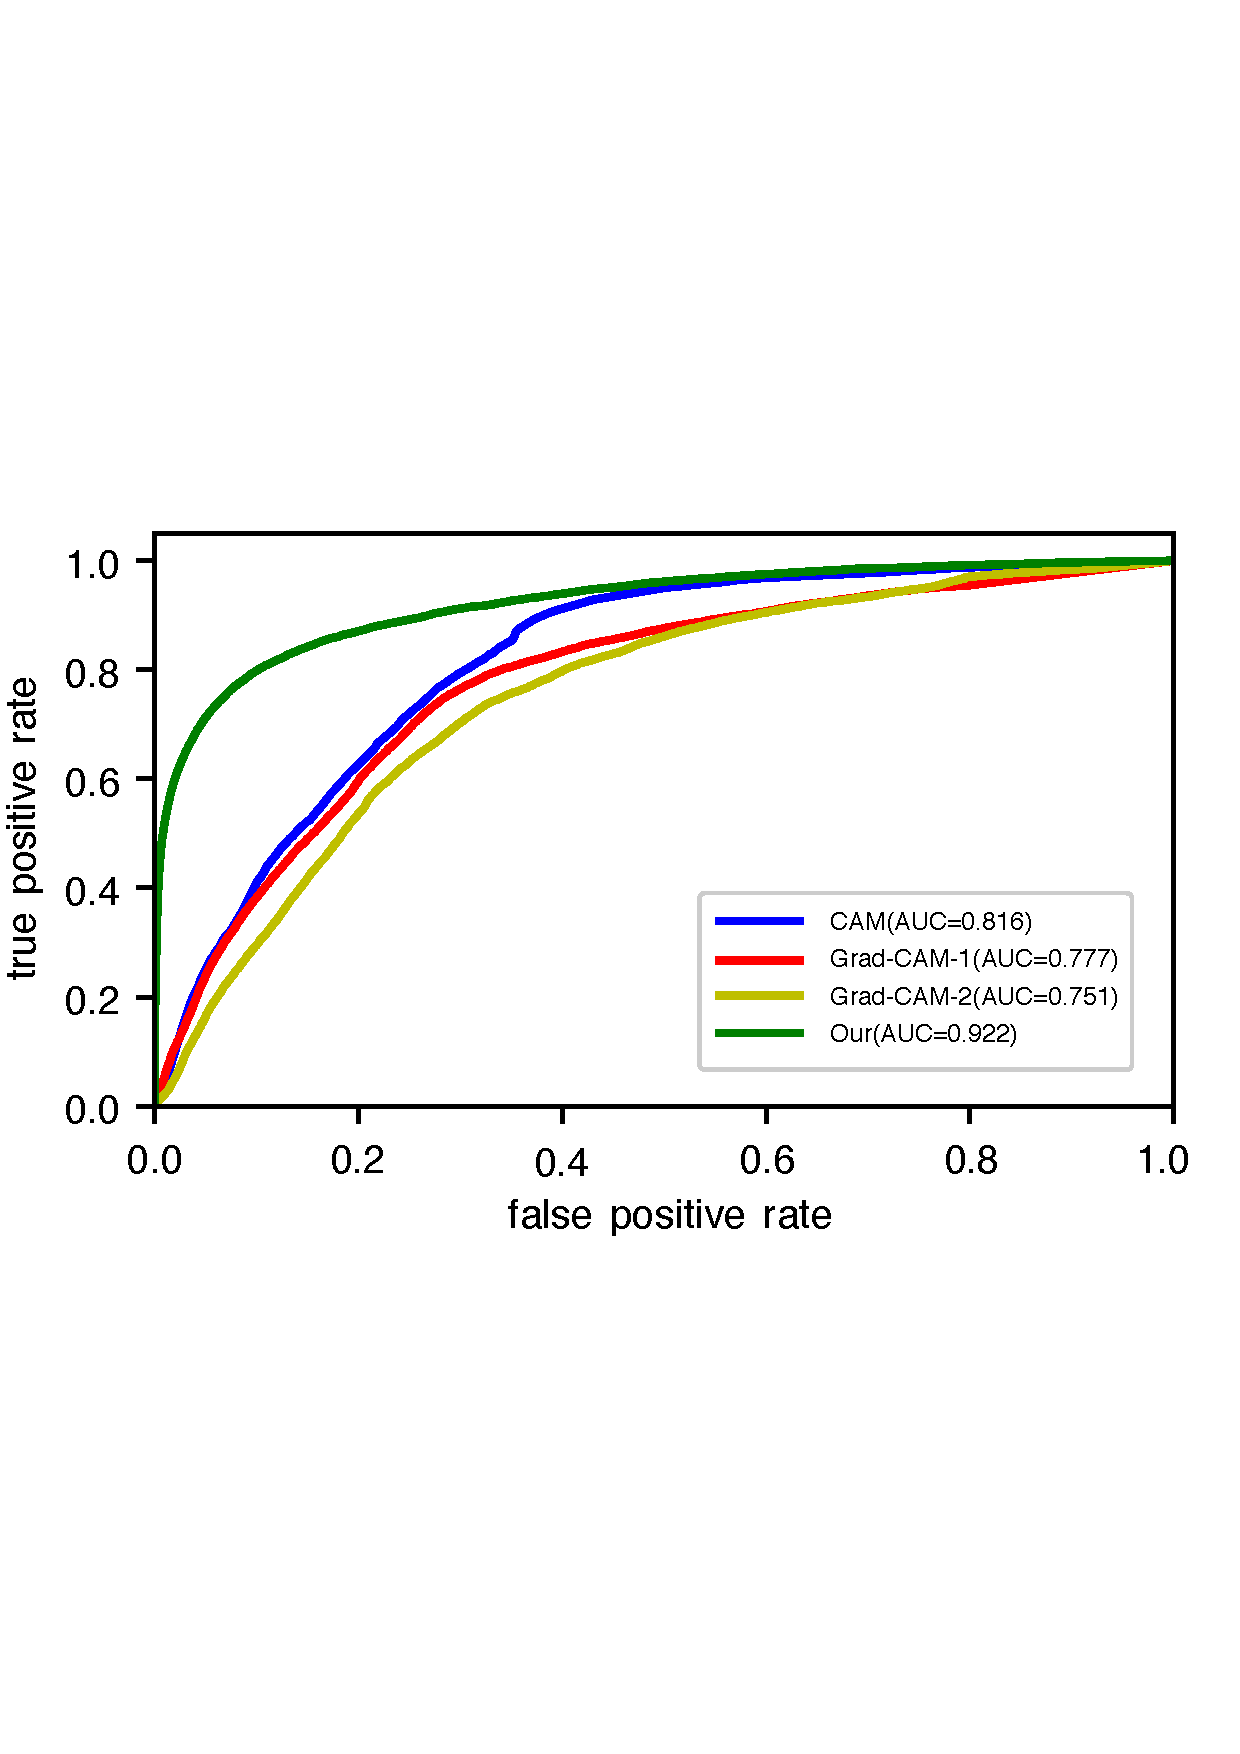
\includegraphics[width=0.7\textwidth]{figure/ROC_cam_grad_cam_our_diabetic_retinopathy}
	\caption[在$40$张视网膜糖尿病病变图像上ROC曲线对比]{在 $40$ 张视网膜糖尿病病变图像上ROC曲线对比。}
	%\caption{CAM、Grad-CAM和本文提出的模型根据二类视网膜糖尿病病变数据集绘制的ROC曲线。ROC曲线是根据数据集中$40$张像素级标注图像绘制。在ROC曲线产生之前,先将各种方法的定位结果的热图归一化到$[0, 1]$。根据P-R曲线及其AUC,与CAM、Grad-CAM相比,本文提出的模型性能表现最佳(AUC最高为$0.922$)。} 
	\label{fig:roc_cam_grad_cam_our_diabetic_retinopathy}
\end{figure}

如图\ref{fig:roc_cam_grad_cam_our_simulated_skin_datasets}所示,CAM、Grad-CAM和本文提出的模型根据二类模拟皮肤病病变数据集绘制的ROC曲线。ROC曲线是根据数据集中所有具有像素级标注的图像绘制。根据P-R曲线及其AUC,与CAM、Grad-CAM相比,本文提出的模型性能表现最佳(AUC最高为$0.933$)。
\begin{figure}[H]
	\centering
	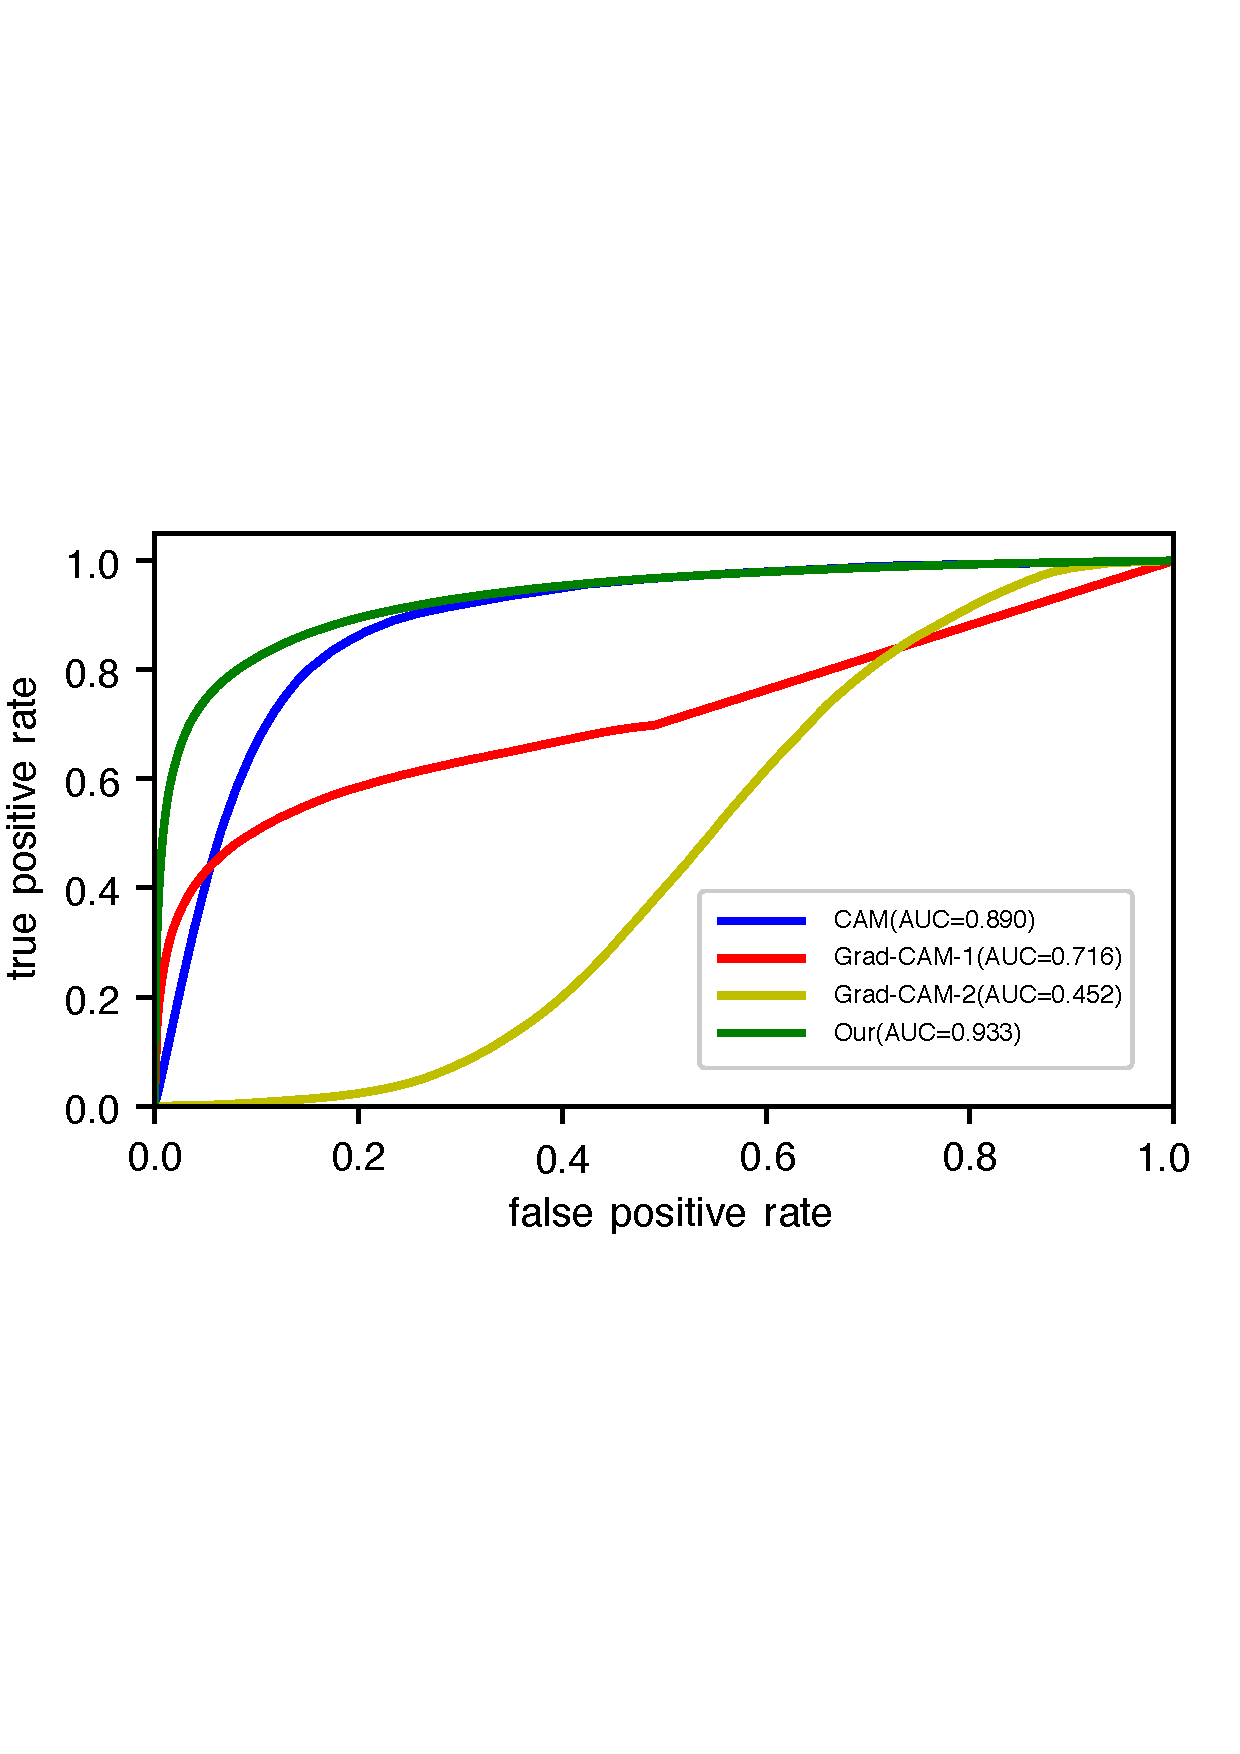
\includegraphics[width=0.7\textwidth]{figure/ROC_cam_grad_cam_our_simulated_skin_datasets}
	\caption[在二类模拟皮肤病病变数据集上ROC曲线对比]{在二类模拟皮肤病病变数据集上ROC曲线对比。}
	
	%\caption{CAM、Grad-CAM和本文提出的模型根据二类模拟皮肤病病变数据集绘制的ROC曲线。ROC曲线是根据数据集中所有具有像素级标注的图像绘制。在ROC曲线产生之前,先将各种方法的定位结果的热图归一化到$[0, 1]$。根据P-R曲线及其AUC,与CAM、Grad-CAM相比,本文提出的模型性能表现最佳(AUC最高为$0.933$)。} 
	\label{fig:roc_cam_grad_cam_our_simulated_skin_datasets}
\end{figure}
%\vspace{-1cm}

如图\ref{fig:roc_u_d_u_c_u_d_c_components}所示,G-D模型、G-C模型和G-D-C模型根据二类视网膜糖尿病病变数据集中标注的部分图像绘制的P-R曲线。G-D-C模型本文提出的完整模型,G-D模型和G-C模型分别表示移去G-D-C模型中的CNN分类器模块和判别器模块得到的子模型。P-R曲线及其AUC表明,与G-D模型和G-C模型相比,G-D-C模型的性能表现最佳(AUC最高为$0.922$)。
\begin{figure}[H]
	\centering
	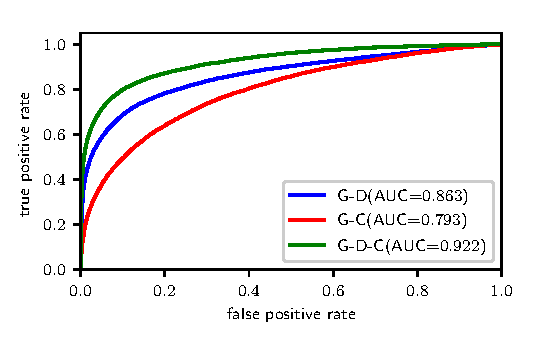
\includegraphics[width=0.7\textwidth]{figure/ROC_u_d_u_c_u_d_c_components}
	\caption[G-D-C模型、G-C模型和G-D模型ROC曲线对比]{在$40$张视网膜糖尿病病变图像上,G-D-C模型、G-C模型和G-D模型ROC曲线对比。}
	%\caption{G-D模型、G-C模型和G-D-C模型根据二类视网膜糖尿病病变数据集中标注的部分图像绘制的P-R曲线。G-D-C模型本文提出的完整模型,G-D模型和G-C模型分别表示移去G-D-C模型中的CNN分类器模块和判别器模块得到的子模型。在ROC曲线产生之前,先将各种方法的定位结果的热图归一化到$[0, 1]$。P-R曲线及其AUC表明,与G-D模型和G-C模型相比,G-D-C模型的性能表现最佳(AUC最高为$0.922$)。}
	\label{fig:roc_u_d_u_c_u_d_c_components}
\end{figure}
\endinput

        %\newclearpage
        % \chapter{多附录}

\section{多附录}


\endinput

        % \newclearpage
   
        %后记
    \backmatter
       %包括硕士期间发表的与毕业论文相关的已发表论文或被鉴定的技术成果、发明专利等成果,应在成果目录中列出。
\chapter{攻读硕士学位期间相关的科研成果目录}

%\setlist[enumerate]{label= \arabic*.}
%\begin{enumerate}
%	\item {\zihao{-4}\heiti 发表论文}
%	\setlist[enumerate]{label= [\arabic*]}
%	\begin{enumerate}
%		\item Rong Zhang, Shuhan Tan, Ruixuan Wang, Siyamalan Manivannan, Jingjing Chen, Haotian Lin, and Wei-Shi Zheng: Biomarker Localization by Combining CNN Classifier and Generative Adversarial Network[C]. Accepted in International Conference on Medical Image Computing and Computer Assisted Intervention (MICCAI 2019). {\zihao{-4}\heiti 已接收(医学影像领域顶会,本人为第一作者)}。
%		\item Weixian Lei$^*$, Rong Zhang$^*$, Yang Yang, Ruixuan Wang, and Wei-Shi Zheng: Class-Center Involved Triplet Loss  for Skin Disease Classification on Imbalanced Data[C]. Accepted in The IEEE International Symposium on Biomedical Imaging (ISBI 2020). {\zihao{-4}\heiti 已接收(医学影像领域高水平会议},\textbf{Best Paper Award Finalist}, {\zihao{-4}\heiti 本人为} {\zihao{-4}\heiti 共同第一作者)。}
%		\item XXX
%	\end{enumerate}
%	\item 发明专利
%	\setlist[enumerate]{label= (\arabic*)}
%	\begin{enumerate}
%		\item XXX
%		\item XXX
%		\item XXX
%	\end{enumerate}
%	\item 获奖
%	\begin{enumerate}
%		\item XXX
%		\item XXX
%		\item XXX
%	\end{enumerate}
%\end{enumerate}

\setlist[enumerate]{label= \arabic*.}
\begin{enumerate}
	\item {\zihao{-4}\heiti 发表论文}
	\setlist[enumerate]{label= [\arabic*]}
	\begin{enumerate}
		\item xxx, xxx, xxx, xxx, xxx, xxx, and xxx: Biomarker Localization by Combining CNN Classifier and Generative Adversarial Network[C]. Accepted in International Conference on Medical Image Computing and Computer Assisted Intervention (MICCAI 2019). {\zihao{-4}\heiti 已发表(医学影像领域国际顶会,本人为第一作者)}。
		\item xxx$^*$, xxx$^*$, xxx, xxx, and xxx: Class-Center Involved Triplet Loss  for Skin Disease Classification on Imbalanced Data[C]. Accepted in The IEEE International Symposium on Biomedical Imaging (ISBI 2020). {\zihao{-4}\heiti 已接收(医学影像领域国际高水平会议},\textbf{Best Paper Award Finalist}, {\zihao{-4}\heiti 本人为} {\zihao{-4}\heiti 共同第一作者)。}
		%		\item XXX
	\end{enumerate}
	%	\item 发明专利
	%	\setlist[enumerate]{label= (\arabic*)}
	%	\begin{enumerate}
	%		\item XXX
	%		\item XXX
	%		\item XXX
	%	\end{enumerate}
	%	\item 获奖
	%	\begin{enumerate}
	%		\item XXX
	%		\item XXX
	%		\item XXX
	%	\end{enumerate}
	
\end{enumerate}    % 科研成果目录
       % \newclearpage
        
       \chapter{致谢}

由衷感谢我的导师某某教授,本文是在他的指导下完成的。……

(谢辞应以简短的文字对课题研究与论文撰写过程中曾直接给予帮助的人员(例如指导教师、答疑教师及其他人员)表示对自己的谢意,这不仅是一种礼貌,也是对他人劳动的尊重,是治学者应当遵循的学术规范。)

\vskip 108pt
\begin{flushright}
	姓名\makebox[1cm]{} \\
	\today
\end{flushright}

    % 致谢
       % \newclearpage
        
       \chapter{中山大学学位论文版权使用授权书}

本学位论文作者及指导教师完全了解“中山大学硕士、博士(硕士)学位论文版权使用规定”,同意中山大学保留并向国家有关部门或机构送交学位论文的复印件和电子版,允许论文被查阅和借阅。本人授权中山大学可以将本学位论文的全部或部分内容编入有关数据库进行检索,也可采用影印、缩印或扫描等复制手段保存和汇编学位论文。

\vskip 108pt
\begin{flushright}
	作者签名:\makebox[2.5cm]{} \\
	导师签名:\makebox[2.5cm]{} \\
	\quad \quad 年 \quad \quad 月 \quad \quad 日
\end{flushright}    % 中山大学学位论文版权使用授权书
       % \newclearpage

\end{document}

